\documentclass[12pt]{article}

% Contains all settings for the document, but more important, a ton of shortcut commands
\usepackage[margin = 1in]{geometry}
\usepackage{amsthm, amsmath, amsfonts, amssymb}
\usepackage{enumerate}
\usepackage{hyperref}
\usepackage{url}
\usepackage{graphicx}

\overfullrule=10pt

\newcommand{\Z}[0]{\mathbb{Z}}
\newcommand{\R}[0]{\mathbb{R}}
\newcommand{\Q}[0]{\mathbb{Q}}
\newcommand{\C}[0]{\mathbb{C}}
\newcommand{\N}[0]{\mathbb{N}}
\newcommand{\D}[0]{\mathbb{D}}
\newcommand{\Om}[0]{\Omega}
\newcommand{\ta}[0]{\theta}
\newcommand{\pp}[0]{\perp}
\newcommand{\bs}[0]{\setminus}
\newcommand{\ld}[0]{\lambda}
\newcommand{\vep}[0]{\varepsilon}
\newcommand{\re}[0]{\operatorname{Re}}
\newcommand{\im}[0]{\operatorname{im}}
\newcommand{\supp}[0]{\operatorname{supp}}
\newcommand{\lsm}[0]{\lesssim}
\newcommand{\pr}[0]{\partial}
\newcommand{\om}[0]{\omega}
\newcommand{\Ld}[0]{\Lambda}
\newcommand{\vp}[0]{\varphi}
\newcommand{\var}[0]{\mathrm{Var}}
\newcommand{\E}[0]{\mathbf{E}}
\newcommand{\pb}[0]{\mathbf{P}}
\newcommand{\cov}[0]{\textrm{Cov}}
\newcommand{\tr}[0]{\mathrm{tr}}
\newcommand{\lap}[0]{\Delta}
\newcommand{\del}[0]{\nabla}
\newcommand{\ba}[0]{\[\begin{aligned}}
\newcommand{\ea}[0]{\end{aligned}\]}
\newcommand{\hq}[0]{\hfill\qed}
\newcommand{\kap}[0]{\kappa}
\newcommand{\sq}[1]{\{#1\}}

\newcommand{\mb}[1]{\mathbf{#1}}
\newcommand{\wh}[1]{\widehat{#1}}
\newcommand{\mc}[1]{\mathcal{#1}}
\newcommand{\mbf}[1]{\mathbf{#1}}
\newcommand{\ov}[1]{\overline{#1}}
\newcommand{\wt}[1]{\widetilde{#1}}
\newcommand{\st}[1]{\substack{#1}}
\newcommand{\sub}[1]{\subsection*{#1}}
\newcommand{\ssb}[1]{\subsubsection*{#1}}

\newcommand{\abs}[1]{\left|#1\right|}
\newcommand{\abb}[1]{\bigg| #1 \bigg|}
\newcommand{\abn}[1]{|#1|}

\newcommand{\nm}[1]{\left\|#1\right\|}
\newcommand{\nmb}[1]{\bigg\| #1 \bigg\|}
\newcommand{\nms}[1]{\| #1 \|}

\newcommand{\ip}[1]{\left\langle #1 \right\rangle}
\newcommand{\ips}[1]{\langle #1 \rangle}
\newcommand{\ipb}[1]{\bigg\langle #1 \bigg\rangle}

\newcommand{\smat}[4]{\left(\begin{smallmatrix} #1 & #2 \\ #3 & #4\end{smallmatrix}\right)}
\newcommand{\svt}[2]{\left(\begin{smallmatrix} #1 \\ #2\end{smallmatrix}\right)}
\newcommand{\pmat}[4]{\begin{pmatrix} #1 & #2 \\ #3 & #4\end{pmatrix}}
\newcommand{\vct}[2]{\begin{pmatrix} #1 \\ #2\end{pmatrix}}

%%%%%%%%%%%%%%%%%%%%%%%%%%%%%%%%%%%%%%%%%%%%%%%%%%%%%%%%%%%%%%%%%%%%%%%%%%%%%%%%%%%%%%%%%%%%%%%

% Calligraphic Symbols
\newcommand{\cA}{\mathcal{A}}
\newcommand{\cB}{\mathcal{B}}
\newcommand{\cC}{\mathcal{C}}
\newcommand{\cD}{\mathcal{D}}
\newcommand{\cE}{\mathcal{E}}
\newcommand{\cF}{\mathcal{F}}
\newcommand{\cG}{\mathcal{G}}
\newcommand{\cH}{\mathcal{H}}
\newcommand{\cI}{\mathcal{I}}
\newcommand{\cJ}{\mathcal{J}}
\newcommand{\cK}{\mathcal{K}}
\newcommand{\cL}{\mathcal{L}}
\newcommand{\cM}{\mathcal{M}}
\newcommand{\cN}{\mathcal{N}}
\newcommand{\cO}{\mathcal{O}}
\newcommand{\cP}{\mathcal{P}}
\newcommand{\cQ}{\mathcal{Q}}
\newcommand{\cR}{\mathcal{R}}
\newcommand{\cS}{\mathcal{S}}
\newcommand{\cT}{\mathcal{T}}
\newcommand{\cU}{\mathcal{U}}
\newcommand{\cV}{\mathcal{V}}
\newcommand{\cW}{\mathcal{W}}
\newcommand{\cX}{\mathcal{X}}
\newcommand{\cY}{\mathcal{Y}}
\newcommand{\cZ}{\mathcal{Z}}

% Vectors --- bolded vectors
\newcommand{\vA}{\textbf{A}}
\newcommand{\vB}{\textbf{B}}
\newcommand{\vC}{\textbf{C}}
\newcommand{\vD}{\textbf{D}}
\newcommand{\vE}{\textbf{E}}
\newcommand{\vF}{\textbf{F}}
\newcommand{\vG}{\textbf{G}}
\newcommand{\vH}{\textbf{H}}
\newcommand{\vI}{\textbf{I}}
\newcommand{\vJ}{\textbf{J}}
\newcommand{\vK}{\textbf{K}}
\newcommand{\vL}{\textbf{L}}
\newcommand{\vM}{\textbf{M}}
\newcommand{\vN}{\textbf{N}}
\newcommand{\vO}{\textbf{O}}
\newcommand{\vP}{\textbf{P}}
\newcommand{\vQ}{\textbf{Q}}
\newcommand{\vR}{\textbf{R}}
\newcommand{\vS}{\textbf{S}}
\newcommand{\vT}{\textbf{T}}
\newcommand{\vU}{\textbf{U}}
\newcommand{\vV}{\textbf{V}}
\newcommand{\vW}{\textbf{W}}
\newcommand{\vX}{\textbf{X}}
\newcommand{\vY}{\textbf{Y}}
\newcommand{\vZ}{\textbf{Z}}
\newcommand{\va}{\textbf{a}}
\newcommand{\vb}{\textbf{b}}
\newcommand{\vc}{\textbf{c}}
\newcommand{\vd}{\textbf{d}}
\newcommand{\ve}{\textbf{e}}
\newcommand{\vf}{\textbf{f}}
\newcommand{\vg}{\textbf{g}}
\newcommand{\vh}{\textbf{h}}
\newcommand{\vi}{\textbf{i}}
\newcommand{\vj}{\textbf{j}}
\newcommand{\vk}{\textbf{k}}
\newcommand{\vl}{\textbf{l}}
\newcommand{\vm}{\textbf{m}}
\newcommand{\vn}{\textbf{n}}
\newcommand{\vo}{\textbf{o}}
%\newcommand{\vp}{\textbf{p}}
\newcommand{\vq}{\textbf{q}}
\newcommand{\vr}{\textbf{r}}
\newcommand{\vs}{\textbf{s}}
\newcommand{\vt}{\textbf{t}}
\newcommand{\vu}{\textbf{u}}
\newcommand{\vv}{\textbf{v}}
\newcommand{\vw}{\textbf{w}}
\newcommand{\vx}{\textbf{x}}
\newcommand{\vy}{\textbf{y}}
\newcommand{\vz}{\textbf{z}}

% Analysis
\newcommand{\indi}{\mathds{1}}
\newcommand{\ep}{\epsilon}

% Differential operators
\renewcommand{\d}{\partial}

% Special functions
\renewcommand{\Re}{\operatorname{Re}}
\renewcommand{\Im}{\operatorname{Im}}
\newcommand{\arcsinh}{\operatorname{arcsinh}}
\newcommand{\arccosh}{\operatorname{arccosh}}
\newcommand{\arctanh}{\operatorname{arctanh}}
\newcommand{\arccsch}{\operatorname{arccsch}}
\newcommand{\arcsech}{\operatorname{arcsech}}
\newcommand{\arccoth}{\operatorname{arccoth}}
\newcommand{\Log}{\operatorname{Log}}
\newcommand{\Si}{\operatorname{Si}}
\newcommand{\sign}{\operatorname{sign}}
\newcommand{\sgn}{\operatorname{sgn}}

% Operator related
\newcommand{\PV}{\operatorname{PV}}

% Linear Algebra
\newcommand{\End}{\operatorname{End}}
\newcommand{\Mat}{\operatorname{Mat}}
\newcommand{\Hom}{\operatorname{Hom}}
\newcommand{\spn}{\operatorname{span}} % Note: not \span
\newcommand{\diag}{\operatorname{diag}}
\newcommand{\rank}{\operatorname{rank}}
\newcommand{\adj}{\operatorname{adj}}
\newcommand{\mult}{\operatorname{mult}} % Note: not \multi

% Define command for average integral (integral with a dash through it)
\def\Xint#1{\mathchoice
{\XXint\displaystyle\textstyle{#1}}%
{\XXint\textstyle\scriptstyle{#1}}%
{\XXint\scriptstyle\scriptscriptstyle{#1}}%
{\XXint\scriptscriptstyle\scriptscriptstyle{#1}}%
\!\int}
\def\XXint#1#2#3{{\setbox0=\hbox{$#1{#2#3}{\int}$}
\vcenter{\hbox{$#2#3$}}\kern-.5\wd0}}
\def\ddashint{\Xint=}
\def\dashint{\Xint-}

% Reporting eigenvalues/eigenvectors of 2x2 matrices - used for phase plane problems
\newcommand{\evev}[6]{\left\{\begin{array}{l} \text{eigenvalue} \,\, \lambda_1 = #1 \,\, \text{with} \,\, \text{eigenvector} \,\, v_1 = \vct{#3}{#4} \\ \vspace*{-0.3cm} \\ \text{eigenvalue} \,\, \lambda_1 = #2 \,\, \text{with} \,\, \text{eigenvector} \,\, v_2 = \vct{#5}{#6} \end{array} \right.}

% Separating rows in arrays
\newcommand{\asep}{\vspace*{-0.3cm} \\}



\newtheorem{claim}{Claim}
\newtheorem*{thm}{Theorem}
\newtheorem{lemma}[claim]{Lemma}
\newtheorem{prop}[claim]{Proposition}
\newtheorem{cor}[claim]{Corollary}

\theoremstyle{remark}
\newtheorem*{rem}{Remark}

\clubpenalty=1000
\widowpenalty=1000



\title{UCLA ADE Qualifying Exam Solutions\\Spring 2007--Spring 2015}
\author{Peter Cheng, Zane Li}
\date{}

\begin{document}

\maketitle

\newpage

\section*{Introduction}
\noindent This is a compendium of solutions of the Applied Differential Equations
qualifying exams dated from Spring 2007 to Spring 2015. This guide
contains solutions to 134 of the 137 questions asked in these 17 exams (the ones missing are Fall 2011 \#1, Spring 2011 \#2, and Fall 2009 \#3).
Sometimes the problem statements contain small errors so we have done our best to modify and solve the problem.
We have tried to be as complete as possible
so as to make the guide relatively self-contained. At the end we have also written up some useful
guides and tricks that we developed as we solved these problems. We hope the reader may find this compendium helpful
in studying. Originally it was planned on typing all the exams from Fall 1999 to Spring 2015, however partially
due to lack of time, we have only been able to type half of them, we have scanned our unedited solutions for Fall 1999--Fall 2006.\\

\noindent While doing the problems, we consulted the guides of
Alejandro Cantarero, Pascal Getreuer, Stuart Harrell, Jeffrey Hellrung, and Joseph Zipkin and so some of
our solutions may be similar to theirs. We also thank the Summer 2015 ADE study group (containing at various
times Yacoub Kureh, Alex Lin, Minh Pham, Michael Puthawala, and Stephanie Wang) for weekly problem discussion.
The phase portraits in this compendium were generated by a Mathematica program written by Yacoub Kureh.\\

\noindent If you spot any errors please contact Peter Cheng or Zane Li.

\section*{Acknowledgements}
\noindent Qi Guo, spotted error in S08\#2


\newpage

\tableofcontents

\newpage

\section{Spring 2015}\label{s15}
\subsection*{Solution to Spring 2015, \# 1}\label{s151}
We mirror the derivation of the Rankine-Hugoniot conditions given in Section 3.4 of Evans.

First assume $v: \R \times [0, \infty) \rightarrow \R$ is smooth with compact support. Then if we pretend
$u$ is a smooth solution to the given conservation law. Since $v$ is of compact support, integration by parts yields
\begin{align*}
0 &= \int_{0}^{\infty}\int_{-\infty}^{\infty}(u_{t} + f(u)_{x} + u)v\, dx\, dt\\
 &= \int_{-\infty}^{\infty}\bigg(-\int_{0}^{\infty}uv_{t}\, dt - uv|_{t = 0}\bigg)\, dx + \int_{0}^{\infty}\bigg(-\int_{-\infty}^{\infty}f(u)v_{x}\, dx\bigg)\, dt + \int_{0}^{\infty}\int_{-\infty}^{\infty}uv\, dx\, dt\\
 &= -\int_{0}^{\infty}\int_{-\infty}^{\infty}uv_{t} + f(u)v_{x} - uv\, dx\, dt - \int_{-\infty}^{\infty}u^{0}(x)v(x, 0)\, dx.
\end{align*}
Thus we define the notion of an integral solution as follows: We say that $u \in L^{\infty}(\R \times (0, \infty))$ is an integral solution
if
\begin{align}\label{s15ran}
-\int_{0}^{\infty}\int_{-\infty}^{\infty}uv_{t} + f(u)v_{x} - uv\, dx\, dt - \int_{-\infty}^{\infty}u^{0}(x)v(x, 0)\, dx = 0
\end{align}
for all smooth $v: \R \times [0, \infty) \rightarrow \R$ with compact support.

Let $V$ be an open region contained in $\R \times (0, \infty)$. Let $V_{\ell}$ be the part of $V$ on the left of a smooth curve $C$
and $V_{r}$ be the part on the right. We assume that $u$ is an integral solution of $u_{t} + f(u)_{x} = -u$ (and so satisfies \eqref{s15ran}) and that
$u$ and its first derivatives are uniformly continuous in $V_{\ell}$ and $V_{r}$.

First, let $\wt{v}$ be a smooth function with compact support in $V_{\ell}$. Then by \eqref{s15ran} since $\wt{v}$ is compactly supported in $V_{\ell} \subset V$,
\begin{align*}
0 = \int_{0}^{\infty}\int_{-\infty}^{\infty}u\wt{v}_{t} + f(u)\wt{v}_{x} - u\wt{v}\, dx\, dt = -\int_{0}^{\infty}\int_{-\infty}^{\infty}(u_{t} + f(u)_{x} + u)\wt{v}\, dx\, dt.
\end{align*}
Therefore since the above equation is true for all smooth $\wt{v}$ with compact support in $V_{\ell}$, we have
$u_{t} + f(u)_{x} + u = 0$ in $V_{\ell}$. Similarly, $u_{t} + f(u)_{x} + u = 0$ in $V_{r}$
(the purpose of this paragraph is to show that if $u$ is an integral solution and is sufficiently smooth,
$u_{t} + f(u)_{x} + u = 0$ in $V_{\ell}$ and $V_{r}$).

Now choose a smooth compactly supported function $v$ with compact support in $V \subset \R \times (0, \infty)$, not necessarily vanishing along
the curve $C$. Again by \eqref{s15ran},
\begin{equation}
\begin{aligned}\label{s15sumint}
0 &= \int_{0}^{\infty}\int_{-\infty}^{\infty}uv_{t} + f(u)v_{x} - uv\, dx\, dt\\
& = \iint_{V_{\ell}}uv_{t} + f(u)v_{x} - uv\, dx\, dt + \iint_{V_{r}}uv_{t} + f(u)v_{x} - uv\, dx\, dt.
\end{aligned}
\end{equation}
Since $v$ has compact support in $V$, integration by parts yields
\begin{equation}
\begin{aligned}\label{s15intleft}
\iint_{V_{\ell}}&uv_{t} + f(u)v_{x} - uv\, dx\, dt\\
 &= -\iint_{V_{\ell}}(u_{t} + f(u)_{x} + u)v\, dx\, dt + \int_{C}(u_{\ell}\nu^{2} + f(u_{\ell})\nu^{1})v\, dl\\
&= \int_{C}(u_{\ell}\nu^{2} + f(u_{\ell})\nu^{1})v\, dl
\end{aligned}
\end{equation}
since $u_{t} + f(u)_{x} + u = 0$ in $V_{\ell}$ where $\nu = (\nu^{1}, \nu^{2})$ is the unit normal to the curve $C$, pointing from $V_{\ell}$ into $V_{r}$
and the subscript $\ell$ denotes the limit from the left. Similarly we have
\begin{align}\label{s15intright}
\iint_{V_{r}}uv_{t} + f(u)v_{x} - uv\, dx\, dt = -\int_{C}(u_{r}\nu^{2} + f(u_{r})\nu^{1})v\, dl.
\end{align}
Adding \eqref{s15intleft} and \eqref{s15intright} and using \eqref{s15sumint}, we have
\begin{align*}
0 = \int_{C}((u_{\ell} - u_{r})\nu^{2} + (f(u_{\ell}) - f(u_{r}))\nu^{1})v\, dl
\end{align*}
for all smooth functions $v$ with compact support in $V$. Therefore
along $C$,
$$(f(u_{r}) - f(u_{\ell}))\nu^{1} + (u_{r} - u_{\ell})\nu^{2} = 0.$$
If we represent $C$ parametrically as $\{(x, t): x = s(t)\}$, then $\nu = (1 + \dot{s}^{2})^{1/2}(1, -\dot{s})$
and hence
$$f(u_{r}) - f(u_{\ell}) = \dot{s}(u_{r} - u_{\ell})$$
along the curve $C$. In the notation of the problem statement, this is
$$f(u_{+}) - f(u_{-}) = \dot{s}(u_{+} - u_{-}).$$
This gives the Rankine-Hugoniot condition along the shock curve $C$.
\hfill\qed

\subsection*{Solution to Spring 2015, \#2}\label{s152}
We will assume that $c$ is differentiable. (Alternatively, the same proof works if we had $\abn{c'(x)} \leq \wh{c}$
instead of $\abn{c(x)} \leq \wh{c}$, because the latter assumption is not really used anywhere.) Let $u, v$ be two compactly
supported smooth solutions to the given PDE. Let $w := u - v$. Then
\begin{align*}
w_{tt} - c(x)^{2}w_{xx} + w_{t} &= 0\quad (x, t) \in \R \times [0, \infty)\\
w(x, 0) &= 0\quad x \in \R\\
w_{t}(x, 0) &= 0\quad x \in \R.
\end{align*}
We mimic the wave energy. Let $$e(t) := \frac{1}{2}\int_{\R}w_{t}^{2} + c(x)^{2}w_{x}^{2}\, dx.$$ Note $e(0) = 0$. We have
\begin{align*}
\dot{e}(t) &= \int_{\R}w_{t}w_{tt} + c(x)^{2}w_{x}w_{xt}\, dx\\
& = \int_{\R}w_{t}w_{tt} - c(x)^{2}w_{xx}w_{t} - 2c(x)c'(x)w_{x}w_{t}\, dx\\
& = \int_{\R}-w_{t}^{2} - 2c(x)c'(x)w_{x}w_{t}\, dx\\
& \leq \int_{\R}-2c'(x)(c(x)w_{x})w_{t}\, dx\\
& \leq 2\|c'\|_{L^{\infty}(\supp w)}\int_{\R}|c(x)w_{x}||w_{t}|\, dx.
\end{align*}
Let $M := 2\|c'\|_{L^{\infty}(\supp w)}$. Then since $ab \leq (a^{2} + b^{2})/2$ for $a, b \geq 0$, it follows that
\begin{align*}
\dot{e}(t) \leq M \cdot \frac{1}{2}\int_{\R}c(x)^{2}w_{x}^{2} + w_{t}^{2}\, dx = Me(t).
\end{align*}
By Gronwall's inequality,
$e(t) \leq e(0)\exp(Mt) = 0$ where the last equality is because $e(0) = 0$. Thus $w_{t} \equiv 0$ and $w_{x} \equiv 0$ which implies $w \equiv 0$ since $w(x, 0) = 0$ for $x \in \R$.
Therefore the PDE has at most one smooth compactly supported solution.
\hfill\qed

\subsection*{Solution to Spring 2015, \#3}\label{s153}
We first solve
\begin{align*}
u_{t} + u_{x}u &= -u\\
u(x, 0) &= x
\end{align*}
as a guide of what we should do in the multidimensional case. In this case we have
\begin{align*}
\begin{array}{ll}
\dot{t}(s) = 1 \quad &t(0) = 0\\
\dot{x}(s) = z \quad &x(0) = x_{0}\\
\dot{z}(s) = -z \quad &z(0) = x_{0}.
\end{array}
\end{align*}
Therefore $t(s) = s$, $z(s) = x_{0}e^{-s}$, and $x(s) = 2x_{0} - x_{0}e^{-s}$.
Thus $x = x_{0}(2 - e^{-t})$ and hence
$$u(x, t) = x_{0}e^{-t} = \frac{e^{-t}x}{2 - e^{-t}} = \frac{x}{2e^{t} - 1}.$$

We now return to the main problem and mimic this argument. We observe that the system can be written as
\begin{align*}
\begin{pmatrix}
u_{1}\\u_{2}
\end{pmatrix}_{t} +
\begin{pmatrix}
(u_{1})_{x_{1}} & (u_{1})_{x_{2}}\\
(u_{2})_{x_{1}} & (u_{2})_{x_{2}}
\end{pmatrix}
\begin{pmatrix}
u_{1}\\ u_{2}
\end{pmatrix} =
-\begin{pmatrix}
u_{1}\\u_{2}
\end{pmatrix}.
\end{align*}
The matrix in the above equation is the Jacobian of $\mathbf{u} = (\begin{smallmatrix}u_{1}\\u_{2}\end{smallmatrix})$ and so is the higher dimensional
analogue of $u_{x}$. We once again have
\begin{align*}
\begin{array}{ll}
\dot{t}(s) = 1 \quad & t(0) = 0\\
\dot{\mathbf{x}}(s) = \mathbf{z} \quad & \mathbf{x}(0) = \mathbf{x_{0}} = \begin{pmatrix}x_{0}^{1}\\x_{0}^{2}\end{pmatrix}\\
\dot{\mathbf{z}}(s) = -\operatorname{Id} \mathbf{z} \quad & \mathbf{z}(0) = \begin{pmatrix}-x_{0}^{2}\\x_{0}^{1}\end{pmatrix}.
\end{array}
\end{align*}
Therefore $t(s) = s$ and
$$\mathbf{z}(s) = \begin{pmatrix} -x_{0}^{2}e^{-s}\\x_{0}^{1}e^{-s}\end{pmatrix}.$$
To find $\mb{x}$, we want to solve $\dot{x_{1}}(s) = -x_{0}^{2}e^{-s}$ and $\dot{x_{2}}(s) = x_{0}^{1}e^{-s}$ and hence combining this with the initial conditions
gives
\begin{align*}
\mb{x}(s) = \pmat{1}{-1}{1}{1}\vct{x_{0}^{1}}{x_{0}^{2}} + \vct{x_{0}^{2}}{-x_{0}^{1}}e^{-s} = \left(\pmat{1}{-1}{1}{1} + \pmat{0}{1}{-1}{0}e^{-s}\right)\vct{x_{0}^{1}}{x_{0}^{2}}
\end{align*}
Therefore
\begin{align*}
\mb{u}(\mb{x}, t) &= \pmat{0}{-1}{1}{0}\vct{x_{0}^{1}}{x_{0}^{2}}e^{-s}\\
& = \pmat{0}{-1}{1}{0}\left(\pmat{1}{-1}{1}{1} + \pmat{0}{1}{-1}{0}e^{-t}\right)^{-1}\vct{x_{1}}{x_{2}}e^{-t}\\
& = \frac{1}{2e^{t} - 2 + e^{-t}}\pmat{1 - e^{-t}}{-1}{1}{1 - e^{-t}}\vct{x_{1}}{x_{2}}.
\end{align*}
\hfill\qed

\subsection*{Solution to Spring 2015, \#4}\label{s154}

\subsubsection*{Solution to $4a$}
Let $u = u_{\ell}1_{(0, 1/2)} + u_{r}1_{(1/2, 1)}$. Then the total variation of $u$ is given by
the supremum of $\int_{0}^{1}u(x)\phi'(x)\, dx$ for differentiable $\phi$ vanishing at both 0 and 1 and $\abn{\phi} \leq 1$.
As
\begin{align*}
\int_{0}^{1}u(x)\phi'(x)\, dx = u_{\ell}\int_{0}^{1/2}\phi'(x)\, dx + u_{r}\int_{1/2}^{1}\phi'(x)\, dx = (u_{\ell} - u_{r})\phi(1/2),
\end{align*}
by the arbitrariness of $\phi$, we have that the total variation of $u$ is given by $\abn{u_{\ell} - u_{r}}$ (with the worse case occurring
when $\phi(1/2) = \pm 1$). Thus in this case,
\begin{align*}
E[u] = \frac{1}{8}\abn{u_{\ell} - u_{r}} + \int_{0}^{1/2}\abn{u_{\ell}}^{2}\, dx + \int_{1/2}^{1} \abn{u_{r} - 1}^{2}\, dx = \frac{1}{8}\abn{u_{\ell} - u_{r}} + \frac{1}{2}u_{\ell}^{2} + \frac{1}{2}(u_{r} - 1)^{2}.
\end{align*}
Thus we wish to minimize
$$f(x, y) := \frac{1}{8}\abn{x - y} + \frac{1}{2}x^{2} + \frac{1}{2}(y - 1)^{2}.$$
We compute
\begin{align*}
f_{x}(x, y) =
\begin{cases}
1/8 + x & \text{ if } x > y\\
-1/8 + x & \text{ if } x < y
\end{cases}
\end{align*}
and
\begin{align*}
f_{y}(x, y) =
\begin{cases}
-9/8 + y & \text{ if } x > y\\
-7/8 + y & \text{ if } x < y.
\end{cases}
\end{align*}
Therefore the critical points for $f(x, y)$ are when $x = y$ (since the derivative does not exist at these points)
and $(1/8, 7/8)$ (note that $(-1/8, 9/8)$ is not a critical point since we have the extra condition that $x > y$ and $-1/8 \not> 9/8$).
Since $f(1/8, 7/8) = 7/64$ and $f(x, x) = x^{2} - x + 1 \geq 3/4$ for all $x$, the piecewise constant function with minimal energy is
$$u = \frac{1}{8}1_{(0, 1/2)} + \frac{7}{8}1_{(1/2, 1)}$$
with $E[u] = 7/64$.
\hfill\qed

\subsubsection*{Solution to $4b$}
We now show that there is no $C^{1}$ function $u$ with energy lower than $7/64$.

Let $u$ be a continuous and almost everywhere differentiable function with minimal energy (we will assume such a minimizer exists).
We avoid working directly with $C^{1}$ functions here to avoid technicalities later (namely, if $u \in C^{1}$, $\max(u, 1)$ is not necessarily in $C^{1}$).
We claim that $u \leq 1$ for every $x$. Let $v(x) := \min(u(x), 1)$. We claim that $E[v] \leq E[u]$. We have
\begin{align*}
E[v] &= \frac{1}{8}\int_{\{u \leq 1\}\cap (0, 1)}|u'|\, dx + \int_{0}^{1}|v - g|^{2}\, dx\\
& = \frac{1}{8}\int_{\{u \leq 1\} \cap (0, 1)}|u'|\, dx + \int_{\{u \leq 1\} \cap (0, 1)}|u - g|^{2}\, dx + \int_{\{u > 1\} \cap (0, 1/2)}1\, dx\\
&\leq \frac{1}{8}\int_{0}^{1}|u'|\, dx + \int_{\{u \leq 1\} \cap (0, 1)}|u - g|^{2}\, dx + \int_{\{u > 1\} \cap (0, 1)}|u - g|^{2}\, dx = E[u]
\end{align*}
where the first inequality is because
\begin{align*}
\int_{\{u > 1\} \cap (0, 1)}|u - g|^{2}\, dx &= \int_{\{u > 1\} \cap (0, 1/2)}|u|^{2}\, dx + \int_{\{u > 1\} \cap (1/2, 1)}|u - 1|^{2}\, dx\\
& \geq \int_{\{u > 1\} \cap (0, 1/2)}1\, dx + \int_{\{u > 1\} \cap (1/2, 1)}|u - 1|^{2}\, dx \geq \int_{\{u > 1\} \cap (0, 1/2)}1\, dx.
\end{align*}
Since $u$ has the smallest energy, we must have $u \leq v$ and hence $u = v = \min(u(x), 1)$ which implies
that $u \leq 1$ everywhere.

Next we claim that $u \geq 0$ for every $x$. Let $w(x) := \max(u(x), 0)$. We claim that $E[w] \leq E[u]$. We have
\begin{align*}
E[w] &= \frac{1}{8}\int_{\{u \geq 0\} \cap (0, 1)}\abn{u'}\, dx + \int_{0}^{1}|w - g|^{2}\, dx\\
&= \frac{1}{8}\int_{\{u \geq 0\} \cap (0, 1)}\abn{u'}\, dx + \int_{\{u \geq 0\} \cap (0, 1)}|u - g|^{2}\, dx + \int_{\{u < 0\} \cap (1/2, 1)}1\, dx\\
&\leq \frac{1}{8}\int_{0}^{1}\abn{u'}\, dx + \int_{\{u \geq 0\} \cap (0, 1)}|u - g|^{2}\, dx + \int_{\{u < 0\} \cap (0, 1)}|u - g|^{2}\, dx = E[u]
\end{align*}
where the first inequality is because
\begin{align*}
\int_{\{u < 0\} \cap (0, 1)}|u - g|^{2}\, dx &= \int_{\{u < 0\} \cap (0, 1/2)}|u|^{2}\, dx + \int_{\{u < 0\} \cap (1/2, 1)}|u - 1|^{2}\, dx\\
&\geq  \int_{\{u < 0\} \cap (0, 1/2)}|u|^{2}\, dx + \int_{\{u < 0\} \cap (1/2, 1)}1\, dx \geq \int_{\{u < 0\} \cap (1/2, 1)}1\, dx.
\end{align*}
Since $u$ has the smallest energy, we must have $u \leq w$ and hence $u = w = \max(u(x) , 0)$ and hence $u \geq 0$ everywhere.

Next we claim that $1 - u(1 -x)$ has the same energy as $u$. Indeed,
\begin{align*}
E[1 - u(1 - x)] &= \frac{1}{8}\int_{0}^{1}|u'(x)|\, dx + \int_{0}^{1}|1 - u(1 - x) - g(x)|^{2}\, dx\\
& = \frac{1}{8}\int_{0}^{1}|u'(x)|\, dx + \int_{0}^{1/2}(1 - u(1 - x))^{2}\, dx + \int_{1/2}^{1}(u(1 - x))^{2}\, dx = E[u]
\end{align*}
where the last equality is by the change of variables $x \mapsto 1 - x$.

Finally, we claim that $u(x) = 1 - u(1 - x)$. Since $E[\,\cdot\,]$ is convex,
\begin{align*}
E[\frac{1 - u(1 - x)}{2} + \frac{u(x)}{2}] \leq \frac{1}{2}E[1 - u(1- x)] + \frac{1}{2}E[u] = E[u].
\end{align*}
Therefore since $u$ has minimal energy, we must have
$$\frac{1 - u(1 - x)}{2} + \frac{u(x)}{2} = u(x),$$
that is, $u(x) = 1 - u(1 - x)$.
Thus we have shown that any minimizer $u$ must satisfy $0 \leq u \leq 1$ and $u(x) = 1 - u(1 - x)$.

Let $m := \min_{x \in [0, 1]}u(x) = u(a)$ and $M := \max_{x \in [0, 1]}u(x) = u(b)$.
Note that
$$M = u(b) = 1 - u(1 - b) \leq 1 - m$$
and
$$1 - m = 1 - u(a) = u(1 - a) \leq M$$
which implies that $M = 1 - m$. Since
$$0 \leq m \leq M = 1 -m \leq 1,$$ we must have $m \in [0, 1/2]$.
Let $I$ denote the interval with endpoints $a$ and $b$. We have
\begin{align*}
\int_{0}^{1}|u'(x)|\, dx \geq \int_{I}|u'(x)|\, dx  \geq \bigg|\int_{I}u'(x)\, dx\bigg| \geq |u(b) - u(a)| = M - m = 1 - 2m
\end{align*}
and
\begin{align*}
\int_{0}^{1}|u(x) - g(x)|^{2}\, dx &= \int_{0}^{1/2}|u(x)|^{2}\, dx + \int_{1/2}^{1}|u(x) - 1|^{2}\, dx\\
& \geq \frac{1}{2}m^{2} + \int_{1/2}^{1}(1 - u(x))^{2}\, dx \geq \frac{1}{2}m^{2} + \frac{1}{2}(1 - M)^{2} = m^{2}
\end{align*}
where in the second inequality we have used that $u \leq 1$.
Therefore
$$E[u] \geq \frac{1}{8}(1 - 2m) + m^{2}$$
with $m\in [0, 1/2]$. Minimizing $(1/8)(1 - 2m) + m^{2}$ over $[0, 1/2]$, we see that $$E[u] \geq \frac{1}{8}(1 - \frac{1}{4}) + \frac{1}{64} = \frac{7}{64}$$
and this occurs when $m = 1/8$. Therefore any continuous energy minimizer $u$ which is also almost everywhere differentiable must have a minimum of $1/8$ and a maximum of $7/8$ and
has energy $\geq 7/64$.

We now construct infinitely many continuous and almost everywhere differentiable functions $u_{n}$ such that $E[u_n]$ is arbitrarily close to $7/64$.
Let
\begin{align*}
u_{n}(x) =
\begin{cases}
1/8 & \text{ if } 0 < x < \frac{1}{2} - \frac{1}{n}\\
L_{n}(x) & \text{ if } \frac{1}{2} - \frac{1}{n} \leq x \leq \frac{1}{2} + \frac{1}{n}\\
7/8 & \text{ if } \frac{1}{2} + \frac{1}{n} < x < 1
\end{cases}
\end{align*}
where $L_n(x)$ is the line created by connecting the points $(\frac{1}{2} - \frac{1}{n}, \frac{1}{8})$
and $(\frac{1}{2} + \frac{1}{n}, \frac{7}{8})$.
Therefore
$$L_{n}(x) = \frac{3n}{8}(x - \frac{1}{2} - \frac{1}{n}) + \frac{7}{8}.$$
Then $u_{n}$ is a continuous and almost everywhere differentiable function.
We compute
\begin{align*}
E[u_{n}] &= \frac{1}{8}\int_{1/2 - 1/n}^{1/2 + 1/n}|L_{n}'|\, dx + \int_{0}^{1/2}|u_{n}|^{2} + \int_{1/2}^{1}|u_{n} - 1|^{2}\, dx\\
&= \frac{6}{64} + \bigg(\frac{1}{2} - \frac{1}{n}\bigg)\frac{1}{64} + \int_{1/2 - 1/n}^{1/2}\bigg(\frac{3n}{8}(x - \frac{1}{2} - \frac{1}{n}) + \frac{7}{8}\bigg)^{2}\, dx\\
&\hspace{1.5in} + \int_{1/2}^{1/2 + 1/n}\bigg(\frac{3n}{8}(x - \frac{1}{2} - \frac{1}{n}) - \frac{1}{8}\bigg)^{2}\, dx + \bigg(\frac{1}{2} - \frac{1}{n}\bigg)\frac{1}{64}\\
&= \frac{6}{64} + \bigg(\frac{1}{2} - \frac{1}{n}\bigg)\frac{1}{64} + \frac{7}{64n} + \frac{7}{64n} + \bigg(\frac{1}{2} - \frac{1}{n}\bigg)\frac{1}{64}\\
& = \frac{7}{64} + \frac{3}{16n}.
\end{align*}

Now suppose there was a $C^{1}$ function $\wt{u}$ with minimal energy. If $E[\wt{u}] > 7/64$, then there exists an $N$ sufficiently large (depending on $\wt{u}$) such that $E[\wt{u}] > E[u_{N}]$,
contradicting minimality of $\wt{u}$. Therefore $E[\wt{u}] \leq 7/64$. But by the above discussion, $\wt{u}$ must have a minimum of $1/8$, a maximum of $7/8$, and
have energy $\geq 7/64$. Therefore $E[\wt{u}] = 7/64$. Thus there is no $C^{1}$ function with energy lower than the optimal piecewise constant function
in part $(a)$.
\hfill\qed

%\subsection*{Solution to Spring 2015, \#5}\label{s155}
%Let $w(x, t) := u(x, t) - v(x, t) - \vep e^{2mt}$. Note that $w(x, 0) < 0$. We claim that $w(x, t) < 0$ for all $t > 0$.
%Suppose not. Then there exists a minimal time $t_{0}$ and a corresponding $x_{0}$ such that $w(x_{0}, t_{0}) = 0$ (as $w(x, 0) < 0$, $w$ is continuous
%and $t_{0}$ is minimal). Since $w(x, t_{0}) \leq 0$ for all $x$, $x_{0}$ is a local maximum for $w(x, t_{0})$ as a function of $x$
%and hence $(\Delta w)(x_{0}, t_{0}) \leq 0$. Since $w(x, t') < 0$ for all $(x, t')$ with $t' < t_{0}$, $w_{t}(x_{0}, t_{0}) \geq 0$. Therefore at $(x_{0}, t_{0})$,
%\begin{align}\label{s155eq1}
%w_{t} - \Delta w \geq 0.
%\end{align}
%However, we compute
%\begin{align*}
%w_{t} - \Delta w = u_{t} - v_{t} - 2M\vep e^{2Mt} - \Delta u + \Delta v = -u^{2} + v^{2} - 2M\vep e^{2Mt}.
%\end{align*}
%Since $w(x_{0}, t_{0}) = 0$, $u(x_{0}, t_{0}) = v(x_{0}, t_{0}) + \vep e^{2Mt_{0}}$. Thus at $(x_{0}, t_{0})$,
%\begin{align*}
%w_{t} - \Delta w &= -(v(x_0, t_0) + \vep e^{2Mt_{0}})^{2} + v(x_{0}, t_{0})^{2} - 2M\vep e^{2Mt_{0}}\\
%& = -2\vep v(x_{0}, t_{0})e^{2Mt_{0}} - \vep^{2}e^{4Mt_{0}} - 2M\vep e^{2Mt_{0}}\\
%& = \vep e^{2Mt_{0}}(-2M - 2v(x_{0}, t_{0}) - \vep e^{2Mt_{0}}) < 0
%\end{align*}
%since $|v(x_{0}, t_{0})| \leq M$. This contradicts \eqref{s155eq1} and hence $w(x, t) < 0$ for all $t > 0$. That is,
%$$u(x, t) < v(x, t) + \vep e^{2Mt}.$$
%Interchanging the role of $u$ and $v$ (and using that $|u| \leq M$) yields that $v(x, t) < u(x, t) + \vep e^{2Mt}$.
%Thus $$\abn{u(x, t) - v(x, t)} < \vep e^{2Mt}.$$
\subsection*{Solution to Spring 2015, \#5}\label{s155}
Define $w(x,t) := u(x,t) - v(x,t) - \epsilon e^{2Mt}$, where $\epsilon$ is from the condition $ |u(x,0) - v(x,0)| < \epsilon$ and $M$ is from $|u|, |v| \leq M$. We aim to show that $w < 0$ for all $(x,t)$. First, observe that
$$ w(x,0) = u(x,0) - v(x,0) - \epsilon < 0 $$
By contradiction, suppose there exists $(x_0,t_0)$ such that $w(x_0,t_0) = 0$. Furthermore, let $t_0$ be the first time for which this happens. Now, consider $w(x,t_0)$ as a function of $x$. Because $w(x,t) < 0 $ for all $x \in \R^n$ and $t < t_0$ and $w(x_0,t_0) = 0$ for all $x \in \R^n$, we have that $w(x,t_0) \leq 0$ for all $x \in \R^n$, implying that $x = x_0$ is a local maximum for $w(x,t_0)$. Hence, $\Delta_x w(x_0,t_0) \leq 0$. We also know that $w_t(x_0,t_0) \geq 0$. Thus, it follows that
$$ (w_t - \Delta_x w)(x_0,t_0) \geq 0 $$
However, at the same time
\begin{align*}
	(w_t - \Delta w)(x_0,t_0) &= (u_t - \Delta u)(x_0,t_0) - (v_t - \Delta v)(x_0,t_0) - 2M \epsilon e^{2M t_0} \\
	&= -u^2 (x_0,t_0) + v^2(x_0,t_0) - 2M \epsilon e^{2Mt_0} \\
	&= -(v(x_0,t_0) + \epsilon e^{2Mt_0})^2 + v^2(x_0,t_0) - 2M \epsilon e^{2Mt_0} \\
	&= -2 \epsilon v(x_0,t_0) e^{2Mt_0} - \epsilon^2 e^{4Mt_0} - 2M \epsilon e^{2Mt_0} \\
	&\leq -\epsilon^2 e^{4Mt_0} \\
	&< 0
\end{align*}
where the third equality is because $w(x_0,t_0) = 0$ and the second-to-last inequality is because $|v| \leq M$. Hence, we have reached a contradiction. Therefore, there does not exist a point $(x_0,t_0)$ such that $w(x_0,t_0) = 0$, and because $w$ is continuous in both variables, we have
$$ w(x,t) < 0 \quad \implies \quad u(x,t) - v(x,t) < \epsilon e^{2Mt} $$
for all $x \in \R^n$ and $t > 0$. If we were to repeat the argument above but with the roles of $u$ and $v$ swapped, meaning we consider the function $y(x,t) := v(x,t) - u(x,t) - \epsilon e^{2Mt}$, we will reach the conclusion
$$ y(x,t) < 0 \quad \implies \quad v(x,t) - u(x,t) < \epsilon e^{2Mt} $$
for all $x \in \R^n$ and $t >0$. Therefore, we have
$$ |u(x,t) - v(x,t)| < \epsilon e^{2Mt} $$
for all $x$ and $t$.
\hfill\qed

\subsection*{Solution to Spring 2015, \#6}\label{s156}
We will denote the Green's function by $G(x, \xi)$ and by $G'(x, \xi)$, we mean $\frac{d}{dx}G(x, \xi)$.
\subsubsection*{Solution to $6a$}
We solve
\begin{align}\label{s156aeq1}
\frac{d^{2}}{dx^{2}}G(x, \xi) - \frac{6}{x^{2}}G(x, \xi) = \delta(x - \xi)
\end{align}
where $G(0, \xi) = 0$ and $G(x, \xi) \rightarrow 0$ as $x \rightarrow \infty$.
The homogenous solutions to $y'' - 6y/x^{2} = 0$ are $x^{3}$ and $x^{-2}$. Therefore
\begin{align*}
G(x, \xi) =
\begin{cases}
ax^{-2} + bx^{3} & \text{ if } x < \xi\\
cx^{-2} + dx^{3} & \text{ if } x > \xi.
\end{cases}
\end{align*}
Since $G(0, \xi) = 0$ and $G(\infty, 0) = 0$, $a = 0$ and $d = 0$.
We also want $G$ to be continuous when $x = \xi$. So we want
$$b \xi^{3} = c\xi^{-2}$$
and hence $c = b\xi^{5}$. If we integrate \eqref{s156aeq1}, then
\begin{align*}
\int_{\xi^{-}}^{\xi^{+}}\frac{d^{2}}{dx^{2}}G(x, \xi)\, dx - \int_{\xi^{-}}^{\xi^{+}}\frac{6}{x^{2}}G(x, \xi)\, dx = \int_{\xi^{-}}{\xi^{+}}\delta(x - \xi)\, dx
\end{align*}
and hence as $G$ is continuous, it follows that $G'(\xi^{+}, \xi) - G'(\xi^{-}, \xi) = 1$. We have
\begin{align*}
G(x, \xi) =
\begin{cases}
bx^{3} & \text{ if } x < \xi\\
b\xi^{5}x^{-2} & \text{ if } x > \xi.
\end{cases}
\end{align*}
Then
\begin{align*}
G'(x, \xi) =
\begin{cases}
3bx^{2} & \text{ if } x < \xi\\
-2b\xi^{5}x^{-3} & \text{ if } x > \xi
\end{cases}
\end{align*}
and hence
\begin{align*}
1 = G'(\xi^{+}, \xi) - G'(\xi^{-}, \xi) = -2b\xi^{2} - 3b\xi^{2} = -5b\xi^{2}.
\end{align*}
Therefore $b = -1/(5\xi^{2})$ and hence
\begin{align*}
G(x, \xi) =
\begin{cases}
-x^{3}/(5\xi^{2}) & \text{ if } x < \xi\\
-\xi^{3}/(5x^{2}) & \text{ if } x > \xi.
\end{cases}
\end{align*}
\hfill\qed

\subsubsection*{Solution to $6b$}
\begin{enumerate}
\item[$(i)$] Since $f$ has a jump discontinuity at $x = 1$, the appropriate continuity conditions for $y$ at $x = 1$ is
\begin{enumerate}
\item $y$ is differentiable at $x = 1$
\item $y'$ is continuous at $x = 1$
\item $y''$ has a jump discontinuity at $x = 1$.
\end{enumerate}
\item[$(ii)$] We have
\begin{align*}
y(x) = \int_{0}^{\infty}G(x, \xi)f(\xi)\, d\xi = \int_{0}^{1}-\frac{x^{3}}{5\xi^{2}}1_{x < \xi} - \frac{\xi^{3}}{5x^{2}}1_{x > \xi}\, d\xi.
\end{align*}
If $x \geq 1$, then
\begin{align*}
 \int_{0}^{1}-\frac{x^{3}}{5\xi^{2}}1_{x < \xi} - \frac{\xi^{3}}{5x^{2}}1_{x > \xi}\, d\xi = -\frac{1}{5x^{2}}\int_{0}^{1}\xi^{3}\, d\xi = -\frac{1}{20x^{2}}.
\end{align*}
If $x < 1$, then
\begin{align*}
 \int_{0}^{1}-\frac{x^{3}}{5\xi^{2}}1_{x < \xi} - \frac{\xi^{3}}{5x^{2}}1_{x > \xi}\, d\xi & = \int_{x}^{1}-\frac{x^{3}}{5\xi^{2}}\, d\xi + \int_{0}^{x}-\frac{\xi^{3}}{5x^{2}}\, d\xi\\
 & = -\frac{x^{3}}{5}\int_{x}^{1}\frac{1}{\xi^{2}}\, d\xi - \frac{1}{5x^{2}}\int_{0}^{x}\xi^{2}\, d\xi = \frac{1}{5}x^{3} - \frac{1}{4}x^{2}.
\end{align*}
Therefore
$$y(x) = \bigg(\frac{1}{5}x^{3} - \frac{1}{4}x^{2}\bigg)1_{x < 1} - \frac{1}{20x^{2}}1_{x \geq 1}.$$
\end{enumerate}
\hfill\qed

\subsection*{Solution to Spring 2015, \#7}\label{s157}
We will assume that $$h(x, t) = a(t)\psi(x/\ell(t))$$ and let $\eta := x/\ell(t)$. Note that in what follows $\psi'(\eta) = d\psi/d\eta$.
Then
\begin{align*}
h_{t} &= a'(t)\psi(\eta) + a(t)\psi'(\eta)x(-\ell(t)^{-2})\ell'(t)\\
& = a'(t)\psi(\eta) - a(t)\psi'(\eta)x\frac{\ell'(t)}{\ell(t)^{2}} = a'(t)\psi(\eta) - a(t)\psi'(\eta)\eta\frac{\ell'(t)}{\ell(t)}.
\end{align*}
Since
$$h_{x} = \frac{a(t)}{\ell(t)}\psi'(\eta) \quad \text{ and } \quad h^{3} = a(t)^{3}\psi(\eta)^{3}$$
it follows that
\begin{align*}
(h^{3}h_{x})_{x} &= \frac{a(t)^{4}}{\ell(t)}(\psi(\eta)^{3}\psi'(\eta))_{x} = \frac{a(t)^{4}}{\ell(t)}(3\psi(\eta)^{2}\psi'(\eta)^{2}\frac{1}{\ell(t)} + \psi(\eta)^{3}\psi''(\eta)\frac{1}{\ell(t)})\\
&=\frac{a(t)^{4}}{\ell(t)^{2}}(3\psi(\eta)^{2}\psi'(\eta)^{2} + \psi(\eta)^{3}\psi''(\eta))
\end{align*}
and hence
\begin{align*}
\frac{1}{3}(h^{3}h_{x})_{x} = \frac{a(t)^{4}}{\ell(t)^{2}}(\psi(\eta)^{2}\psi'(\eta)^{2} + \frac{1}{3}\psi(\eta)^{3}\psi''(\eta)).
\end{align*}
Since $h_{t} = \frac{1}{3}(h^{3}h_{x})_{x}$, we have
\begin{align}\label{s157eq1}
\frac{\ell(t)^{2}}{a(t)^{4}}\bigg(a'(t)\psi(\eta) - a(t)\psi'(\eta)\eta\frac{\ell'(t)}{\ell(t)}\bigg) = \psi(\eta)^{2}\psi'(\eta)^{2} + \frac{1}{3}\psi(\eta)^{3}\psi''(\eta).
\end{align}
Let $a(t) := t^{\alpha}$ and $\ell(t) := t^{\beta}$. Then
\begin{align*}
\frac{\ell(t)^{2}}{a(t)^{4}}a'(t) = \alpha t^{2\beta - 3\alpha - 1}
\end{align*}
and
\begin{align*}
\frac{\ell(t)^{2}}{a(t)^{4}}a(t)\frac{\ell(t)}{\ell'(t)} = \frac{\ell(t)}{a(t)^{3}}\ell'(t) = \beta t^{2\beta - 3\alpha - 1}.
\end{align*}
Balancing powers of $t$ in \eqref{s157eq1}, we must have
\begin{align}\label{s157eq2}
2\beta - 3\alpha = 1.
\end{align}
With this condition on $\alpha$ and $\beta$, this changes \eqref{s157eq1} into
\begin{align}\label{s157eq3}
\alpha\psi(\eta) - \beta\psi'(\eta)\eta = \psi(\eta)^{2}\psi'(\eta)^{2} + \frac{1}{3}\psi(\eta)^{3}\psi''(\eta).
\end{align}
We now use the boundary conditions to give another relation between $\alpha$ and $\beta$.
We have
\begin{align*}
1 = \int_{-L(t)}^{L(t)}h(x, t)\, dx = \int_{-L(t)}^{L(t)}t^{\alpha}\psi(x/t^{\beta})\, dx = \int_{-L(t)/t^{\beta}}^{L(t)/t^{\beta}}t^{\alpha + \beta}\psi(s)\, ds
\end{align*}
and hence
\begin{align*}
\int_{-L(t)/t^{\beta}}^{L(t)/t^{\beta}}\psi(s)\, ds = t^{-\alpha - \beta}.
\end{align*}
Taking the time derivative of both sides gives
\begin{align*}
\psi(\frac{L(t)}{t^{\beta}})\frac{d}{dt}(\frac{L(t)}{t^{\beta}}) - \psi(-\frac{L(t)}{t^{\beta}})\frac{d}{dt}(-\frac{L(t)}{t^{\beta}}) = (-\alpha - \beta)t^{-\alpha - \beta - 1}.
\end{align*}
Since $h(\pm L(t), t) = 0$,
$$0 = t^{\alpha}\psi(\pm\frac{L(t)}{t^{\beta}})$$
and hence $\psi(\pm L(t)/t^{\beta}) = 0$.
Therefore we must also have
\begin{align}\label{s157eq4}
-\alpha - \beta = 0.
\end{align}
Combining \eqref{s157eq2} and \eqref{s157eq4} gives that
$$\alpha = -1/5 \quad \text{ and } \quad \beta = 1/5.$$
Then \eqref{s157eq3} becomes
\begin{align*}
-\frac{1}{5}\psi(\eta) - \frac{1}{5}\psi'(\eta)\eta &= \psi(\eta)^{2}\psi'(\eta)^{2} + \frac{1}{3}\psi(\eta)^{3}\psi''(\eta)\\
-(\psi(\eta) + \psi'(\eta)\eta) &= 5\psi(\eta)^{2}\psi'(\eta)^{2} + \frac{5}{3}\psi(\eta)^{3}\psi''(\eta)
\end{align*}
and hence
\begin{align*}
-(\eta\psi(\eta))' &= (\frac{5}{3}\psi(\eta)^{3}\psi'(\eta))'.
\end{align*}
Therefore
$$-\eta\psi(\eta) = \frac{5}{3}\psi(\eta)^{3}\psi'(\eta) + C.$$
Take $\eta = L(t)/t^{1/5}$. Then with this choice of $\eta$, $\psi(\eta) = 0$ and hence $C = 0$. Thus
$$-\eta\psi(\eta) = \frac{5}{3}\psi(\eta)^{3}\psi'(\eta).$$
This equation is now separable. Solving yields
\begin{align*}
-\frac{1}{2}\eta^{2} = \frac{5}{9}\psi^{3} + \wt{C}.
\end{align*}
Take $\eta = L(t)/t^{1/5}$, then $$\wt{C} = -\frac{1}{2}\bigg(\frac{L(t)}{t^{1/5}}\bigg)^{2} = -\frac{1}{2}\cdot \frac{L^{2}}{t^{2/5}}.$$
Therefore
$$\frac{5}{9}\psi^{3} = \frac{1}{2}\bigg(\frac{L^{2}}{t^{2/5}} - \eta^{2}\bigg)$$
and hence
$$\psi(\eta) = \bigg(\frac{9}{10}\bigg)^{1/3}\bigg(\frac{L^{2}}{t^{2/5}} - \eta^{2}\bigg)^{1/3}.$$
Since $\eta = x/\ell(t) = x/t^{1/5}$,
\begin{align*}
h(x, t) = t^{-1/5}\bigg(\frac{9}{10}\bigg)^{1/3}\bigg(\frac{L^{2}}{t^{2/5}} - \frac{x^{2}}{t^{2/5}}\bigg)^{1/3} = \bigg(\frac{9}{10}\bigg)^{1/3}t^{-1/3}(L^{2} - x^{2})^{1/3}.
\end{align*}
Now we compute $L(t)$. Since $\int_{-L(t)}^{L(t)}h(x, t)\, dx = 1$,
\begin{align*}
\bigg(\frac{9}{10t}\bigg)^{1/3}\int_{-L}^{L}(L^{2} - x^{2})^{1/3}\, dx = 1.
\end{align*}
Rearranging and making the change of variables $x = L\sin\ta$ yields that
\begin{align*}
\bigg(\frac{10t}{9}\bigg)^{1/3} = L\int_{-\pi/2}^{\pi/2}(\cos^{2/3}\ta)\cos \ta\, d\ta = 2L\int_{0}^{\pi/2}\cos^{5/3}\ta\, d\ta.
\end{align*}
Therefore
$$L(t) = \bigg(\frac{10t}{9}\bigg)^{1/3}\bigg(2\int_{0}^{\pi/2}\cos^{5/3}\ta\, d\ta\bigg)^{-1}$$
and
$$h(x, t) = \bigg(\frac{9}{10t}\bigg)^{1/3}(L^{2} - x^{2})^{1/3}.$$
\hfill\qed

\subsection*{Solution to Spring 2015, \#8}\label{s158}
\subsubsection*{Solution to $8a$}
The equilibrium points are
$$(x, y) = (0, 0), (1, 1), (-1, -1), (1, -1), (-1, 1).$$
The Jacobian is
$$J(x, y) = \pmat{1 - y^{2}}{-2xy}{-2xy}{1 - x^{2}}.$$
The Jacobian at $(0, 0)$ is $\smat{1}{0}{0}{1}$, the Jacobian at $(1, 1)$ and $(-1, -1)$
is $\smat{0}{-2}{-2}{0}$, and the Jacobian at $(1, -1)$ and $(-1, 1)$ is $\smat{0}{2}{2}{0}$.

The eigenvalues of $\smat{1}{0}{0}{1}$ are $1, 1$ and the eigenvectors are $\svt{1}{0}$ and $\svt{0}{1}$.
The eigenvalues of $\smat{0}{-2}{-2}{0}$ are $2, -2$ and the corresponding eigenvectors are $\svt{1}{-1}$ and
$\svt{1}{1}$. The eigenvalues of $\smat{0}{2}{2}{0}$ are $2, -2$ and the corresponding eigenvectors are $\svt{1}{1}$ and $\svt{1}{-1}$.
Therefore $(0, 0)$ is a source node and $(\pm 1, \pm 1)$ are all saddles.
The phase portrait is as follows:

\begin{center}
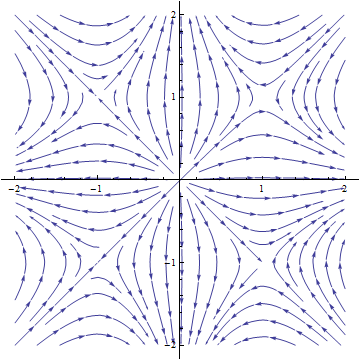
\includegraphics[scale=0.75]{./_Figures/S158.png}
\end{center}

For large $x, y$, $1 - y^{2} \approx -y^{2}$ and $1 - x^{2} \approx -x^{2}$. Then
\begin{align*}
\frac{dy}{dx} \approx \frac{x}{y}
\end{align*}
and hence for large $x$ and large $y$, the trajectories looks like $x^{2} - y^{2} = C$, in other words, the trajectories for large $x$, $y$
are hyperbolas.
\hfill\qed

\subsubsection*{Solution to $8b$}
The Jacobian in this case is
$$J(x, y) = \pmat{1 - y^{2}}{-2xy}{-2xy^{2}}{2y(1 - x^{2})}$$
and so $J(1, -1) = \smat{0}{2}{-2}{0}$ which has eigenvalues $\pm 2i$. Therefore $(1, -1)$ is either a center or spiral.
To prove $(1, -1)$ is stable, we use Lyapunov theory. We solve
$$\frac{dy}{dx} = \frac{y^{2}(1 - x^{2})}{x(1 - y^{2})}$$
which yields
$$-\frac{1}{y} - y = \log x - \frac{1}{2}x^{2} + C.$$
Let $$V(x, y) = \frac{1}{2}x^{2} - \log x - \frac{1}{y} - y - \frac{5}{2}.$$
Then $V(1, -1) = 0$. Note that
$$\dot{V}(x, y) = x\dot{x} - \frac{1}{x}\dot{x} + \frac{1}{y^{2}}\dot{y} - \dot{y} = x^{2}(1 - y^{2}) - (1 - y^{2}) + 1 - x^{2} - y^{2}(1 - x^{2}) = 0.$$
Since
$$V(x, y) = (\frac{1}{2}x^{2} - x + \frac{1}{2}) + (x - 1 - \log x) + (-2 - \frac{1}{y} - y)$$
and each piece is $> 0$ for some sufficiently small neighborhood of $(1, -1)$, it follows from Lyapunov's theorem
(Page 363 of Jordan-Smith, Third Edition) that $(1, -1)$ is uniformly stable, so is stable.

An alternative solution can be fashioned as follows. Let
$$E(x, y) := \frac{1}{2}x^{2} - \log x - \frac{1}{y} - y.$$
Then $E$ is an ``energy" that is conserved by the system. Since $(1, -1)$ is a local minimum for $E(x, y)$, by Theorem 6.5.1 on Page 163 of
Strogatz's Nonlinear Dynamics and Chaos, Second Edition, it follows that $(1, -1)$ is a center and hence stable.
(The moral here is that if one can find a conserved quantity for the system and the equilibrium point is an isolated
equilibrium point, then the trajectories around said equilibrium point are closed.)
\hfill\qed


\section{Fall 2014}\label{f14}
\subsection*{Solution to Fall 2014, \#1}
\label{F14Q1}

\subsubsection*{Solution to $1a$}

The system of ODEs represents a predator-prey system. For the species represented by $x$, the $2x$ term represents growth for the species, the $-x^2$ term represents a decay of the species, and the $-xy$ term represents competition between species $x$ and $y$. For the species represented by $y$, the $y$ term represents growth for the species, and the $-xy$ term represents competition between species $x$ and $y$.

\subsubsection*{Solution to $2a$}

Setting $\dot{x}$ and $\dot{y}$ equal to 0 yields the following fixed points: $(0,0), (1,1), (2,0)$. Define $F(x,y) := (2x-x^2-xy, y-xy)$, and compute the Jacobian
$$ J[F](x,y) = \pmat{2-2x-y}{-x}{-y}{1-x} $$
Then, we compute eigenvalues and eigenvectors:
$$ J[F](0,0) = \pmat{2}{0}{0}{1} \quad \implies \quad \evev{2}{1}{1}{0}{0}{1}$$
$$ J[F](1,1) = \pmat{-1}{-1}{-1}{0}  \implies\evev{\frac{-1+\sqrt{5}}{2}}{\frac{-1-\sqrt{5}}{2}}{1-\sqrt{5}}{2}{1+\sqrt{5}}{2} $$
$$ J[F](2,0) = \pmat{-2}{-2}{0}{-1}\quad \implies \quad \evev{-2}{-1}{1}{0}{-2}{1} $$
Below is a plot of the phase plane.

\begin{center}
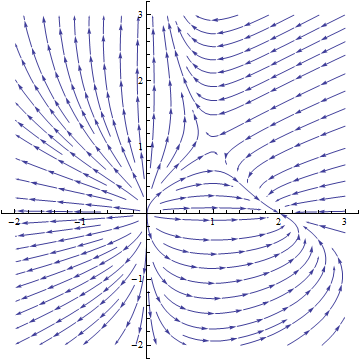
\includegraphics[scale=0.75]{./_Figures/f141_ppp.png}
\end{center}

The nullclines are the contours $2x-x^2-xy=0$ and $y-xy=0$, which are not shown in the plot above.
For large $x, y$, $\dot{x} \approx -x^{2} - xy$ and $\dot{y} \approx -xy$ and hence
$$\frac{dx}{dy} \approx \frac{-x - y}{-y} = 1 + \frac{x}{y}.$$
Therefore
$$\frac{dx}{dy} - \frac{x}{y} - 1 = 0.$$
Dividing both sides by $y$ yields that
$$\frac{d}{dy}\left(\frac{1}{y}x\right) = \frac{1}{y}$$
which gives $x = y\log y + Cy$. Therefore the trajectories look like
$x = y\log y + Cy$ for $x, y$ large.





\subsection*{Solution to Fall 2014, \#2}
\label{F14Q2}

\subsubsection*{Solution to $2a$}

We are looking to find $y$ and $\lambda$ such that
\[
x^2 y'' + x y' + \lambda y = 0, \quad \text{where} \quad y(1) = y(2) = 0
\]
First, observe notice $\lambda \neq 0$. If $\lambda$ were zero, then
\[
x^2 y'' + xy' = 0 \quad \implies \quad y' = \frac{C}{x} \quad \implies \quad y = C \ln(x) + D
\]
for constants $C$ and $D$ However, this solution doesn't satisfy the boundary conditions unless $y \equiv 0$, implying $\lambda = 0$ is not an eigenvalue.

With the ansatz $y = x^n$, observe
\[
x^2 y'' + x y' + \lambda y = n(n-1)x^n + n x^n + \lambda x^n = 0 \quad \implies \quad n^2 = - \lambda
\]
If $\lambda < 0$, then $n = \pm \sqrt{-\lambda}$, and
\[
y= A x^{\sqrt{-\lambda}} + Bx^{-\sqrt{-\lambda}}
\]
The only choice of constants $A$ and $B$ such that $y$ satisfies the boundary conditions is $A = B = 0$, so any choice of $\lambda < 0$ is not an eigenvalue. 						

If $\lambda > 0$, then $n = \pm i \sqrt{\lambda}$, and
\[
x^{\pm i \sqrt{n}} = \cos(\sqrt{\lambda} \ln(x)) \pm i \sin(\sqrt{\lambda} \ln (x))
\]
Hence,
\[
y = A \cos ( \sqrt{\lambda} \ln (x)) + B \sin( \sqrt{\lambda} \ln (x))
\]
In order for $y$ to satisfy the boundary conditions, we get $A=0$ and $\lambda = \left( \frac{k \pi}{\ln 2} \right)^2$ for $k > 1$. Thus it follows the eigenfunctions are
\[
\mu_k(x) = \sin \left( \frac{k \pi \ln x}{\ln 2} \right)
\]
with associated eigenvalue $\lambda_k =  \left( \frac{k \pi}{\ln 2} \right)^2$. \hfill \qed

\subsubsection*{Solution to $2b$}

In order to use our previous work to our advantage, we first show that ODE is a Sturm-Liouville problem. Indeed,
\[
x^2 y'' + xy' + \lambda y = 0 \quad \implies \quad x [ (xy')'] = -\lambda y
\]
which is now in Sturm-Liouville form. Thus, the operator $Ly := x[(xy')']$ is self-adjoint with respect to the weighted inner product $<u,v>_{r(x)} = \int_1^2 u(x)v(x) r(x) \, dx$, where $r(x) = \frac{1}{x}$. This implies that the set of eigenfunctions $\{ \mu_k(x) \}$ for $k > 1$ forms an orthogonal basis. Now, the solution $y$ to
\[
x^2 y'' + x y' + 3y = x \log x \quad \text{where} \quad y(1) = y(2) = 0
\]
can be represented as
\begin{equation}
\label{F14Q2Eq1}
y(x) = \sum_{k=1}^{\infty} a_k \mu_k(x)
\end{equation}
Before solving for $a_k$, observe
\begin{equation}
\label{F14Q2Eq2}
x^2 y'' + x y' + 3y = x \log x \quad \implies \quad (L + 3I) y = x \log x
\end{equation}
where $L$ is defined above and $I$ is the identity operator. Because the eigenfunctions form an orthogonal basis, we may also write
\[
x \log x = \sum_{k=1}^{\infty} f_k \mu_k(x) \quad \text{where} \quad f_k = \dfrac{\int_1^2 \log (x) \mu_k(x) \, dx}{\int_1^2 \mu_k(x)^2 r(x) \, dx}
\]
Now, plugging \eqref{F14Q2Eq1} into \eqref{F14Q2Eq2} yields
\begin{align*}
(L + 3I) \left( \sum_{k=1}^{\infty} a_k \mu_k(x) \right) = \sum_{k=1}^{\infty} f_k \mu_k(x) \quad &\implies \quad \sum_{k=1}^{\infty} a_k (\lambda_k + 3) \mu_k (x) = \sum_{k=1}^{\infty} f_k \mu_k(x) \\
&\implies \quad a_k = \frac{f_k}{\lambda_k + 3}
\end{align*}
Therefore, the solution is
\[
y(x) = \sum_{k=1}^{\infty} \frac{f_k}{\lambda_k+3} \mu_k(x) \quad \text{where} \quad f_k = \dfrac{\int_1^2 \log (x) \mu_k(x) \, dx}{\int_1^2 \mu_k(x)^2 r(x) \, dx}
\]
Note that there are no solutions to the homogeneous version of this ODE. If there were, then $\lambda = 3$ would be an eigenvalue of the ODE in part (a), which is a contradiction to our work above. \hfill \qed


\subsection*{Solution to Fall 2014, \#3}
\label{F14Q3}

\subsubsection*{Solution to $3a$}

We solve this using method of characteristics. Since the PDE is quasilinear, we only need the following three ODEs to solve the PDE:
\begin{align}
\label{f143t} &\dot{t}(s) = 1, \quad t(0) = 0 \\
\label{f143x} &\dot{x}(s) = z(s), \quad x(0) = x_0 \\
\label{f143z} &\dot{z}(s) = 0, \quad z(0) = \cos(x_0)
\end{align}
Solving \eqref{f143t} and \eqref{f143z} yield
$$ t(s) = s, \quad \text{and} \quad z(s) = z(t) = \cos(x_0) $$
respectively. Then, solving for \eqref{f143x} yields
$$ x(s) = x(t) = \cos(x_0) t + x_0 $$
Therefore, $u(x,t) = \cos(x_0)$ where $x = \cos(x_0)t + x_0$. \hfill \qed

\subsubsection*{Solution to $3b$}

First, note that our solution won't be continuous for all time. To see this, consider two characteristics that start at $a$ and $b$, where $a \neq b$ and $\cos(a) \neq \cos(b)$. These two characteristics will intersect when
$$ \cos(a) t + a = \cos(b) t + b \quad \implies \quad t = \frac{b-a}{\cos(a) - \cos(b)} $$
However, this analysis is not entirely accurate. Since the characteristics are straight lines that are not all parallel, we can find $c$ where $a < c < b$ such that the characteristic starting at $c$ will crash into either the characteristic starting at $a$ or $b$ first. At this point, we either (1) stop defining our solution because we want something that's continuous, or (2) apply the Rakine-Hugoniot condition to figure out the shock curve that starts at the crash. Either way, this implies that the characteristics starting at $a$ and $b$ will never crash as long as $a \neq b$ and $\cos(a) \neq \cos(b)$. Hence, we must examine characteristics that start arbitrarily close to each other in order to obtain accurate data about them intersecting.

Letting $b$ tend to $a$ yields $t = 1/\sin(a)$. Hence, if we let $a = \pi/2$, we now know that characteristics that start arbitrarily close to $\pi/2$ will crash close to $t=1$, which is the smallest time for which discontinuities in our solution will occur.

For $t < 1$, our solution is continuous. Furthermore, along the characteristic that starts at $x_0 = 0$, $u(x,t) = 1$. Because of the behavior of cosine, we know that $u(x,t) \leq 1$, which implies $\max_{x \in \R} u(x,t) = 1$. \hfill \qed






\subsection*{Solution to Fall 2014, \#4}
\label{F14Q4}

\subsubsection*{Solution to $4a$}

Let $v \in H^1_0((0,1))$ be an arbitrary test function. Then, integration by parts yields
$$ \int_0^1 \d_x(\beta u_x) v \, dx = \int_0^1 fv \, dx \quad \implies \quad -\int_0^1 \beta u_x v_x \, dx = \int_0^1 fv \, dx $$
which is the weak form. Note that $\beta u_x$ is continuous at $\hat{x}$, so we don't need to split up the integral at $\hat{x}$. Furthermore, because $v$ vanishes at the endpoints, the boundary terms vanish.

\subsubsection*{Solution to $4b$}

We first construct the Green's function for the case where $x_0 < \hat{x}$. For $x \neq x_0$, the ODE boils down to
$$
-\frac{\d}{\d x} \left( \beta(x) G_x(x;x_0) \right) = 0 \quad \implies \quad G(x;x_0) = \left\{
\begin{array}{ll}
a_1 + a_2 x & \text{if} \,\, 0 \leq x < x_0 \\
b_1 + b_2 x & \text{if} \,\, x_0 < x < \hat{x} \\
c_1 + c_2 x & \text{if} \,\, \hat{x} < x \leq 1
\end{array} \right.
$$
where $a_1, a_2, b_1, b_2, c_1, c_2$ are constants. From the conditions of our problem, we have
\begin{align}
\label{f1441} &G(0,x_0) = G(1,x_0) = 0 \quad \implies \quad a_1 = 0, \,\,\, c_1 + c_2 = 0 \\
\label{f1442} &G(\hat{x}^+,x_0) = G(\hat{x}^-,x_0) \quad \implies \quad c_1 + c_2 \hat{x} = b_1 + b_2 \hat{x} \\
\label{f1443} &\beta(\hat{x}^+)G_x(\hat{x}^+,x_0) = \beta(\hat{x}^-)G_x(\hat{x}^-,x_0) \quad \implies \quad 2c_2 = b_2
\end{align}
We also have
$$ \int_{x_0^-}^{x_0^+} -\frac{\d}{\d x} \left( \beta(x) G_x(x,x_0) \right) \, dx = \int_{x_0^-}^{x_0^+} \delta(x-x_0) \, dx = 1 $$
Since $x_0 < \hat{x}$, this implies
\begin{equation}
\label{f1444} G_x(x_0^+,x_0) - G_x(x_0^-, x_0) = -1 \quad \implies \quad b_2 - a_2 = -1
\end{equation}
We also need $G(x,x_0)$ to be continuous at $x=x_0$, so we want
\begin{equation}
\label{f1445} a_2 x_0 = b_1 + b_2 x_0
\end{equation}
Solving \eqref{f1441} through \eqref{f1445} yields the following Green's function for $x_0 < \hat{x}$
$$ G(x,x_0) =
\left\{
\begin{array}{ll}
\left( 1 -\dfrac{2x_0}{\hat{x}+1} \right) x & \text{if} \,\,\, 0 \leq x < x_0 \\ \asep
x_0 - \dfrac{2x_0}{\hat{x}+1} x & \text{if} \,\,\, x_0 < x < \hat{x} \\ \asep
\dfrac{x_0}{\hat{x}+1} (1-x) & \text{if} \,\,\, \hat{x} < x \leq 1
\end{array}
\right. $$
For $x_0 > \hat{x}$, we now have
$$ G(x;x_0) = \left\{
\begin{array}{ll}
a_1 + a_2 x & \text{if} \,\, 0 \leq x < \hat{x} \\
b_1 + b_2 x & \text{if} \,\, \hat{x} < x < x_0 \\
c_1 + c_2 x & \text{if} \,\, x_0 < x \leq 1
\end{array} \right.
$$
with the conditions
\begin{align}
\label{f1446} &G(0,x_0) = G(1,x_0) = 0 \quad \implies \quad a_1 = 0, \,\,\, c_1 + c_2 = 0 \\
\label{f1447} &G(\hat{x}^+,x_0) = G(\hat{x}^-,x_0) \quad \implies \quad b_1 + b_2 \hat{x} = a_1 + a_2 \hat{x} = a_2 \hat{x} \\
\label{f1448} &\beta(\hat{x}^+)G_x(\hat{x}^+,x_0) = \beta(\hat{x}^-)G_x(\hat{x}^-,x_0) \quad \implies \quad 2b_2 = a_2 \\
\label{f1449} &G_x(x_0^+,x_0) - G_x(x_0^-, x_0) = -\dfrac{1}{2} \quad \implies \quad c_2 - b_2 = -\dfrac{1}{2} \\
\label{f14410} &G(x_0^-,x_0) = G(x_0^+,x_0) \quad \implies \quad b_1 + b_2 x_0 = c_1 + c_2 x_0
\end{align}
Solving \eqref{f1446} through \eqref{f14410} yields the following Green's function for $x_0 > \hat{x}$
$$ G(x,x_0) =
\left\{
\begin{array}{ll}
\dfrac{1-x_0}{\hat{x}+1} x & \text{if} \,\,\, 0 \leq x < \hat{x} \\ \asep
\dfrac{1}{2}(1-x_0) \left( \dfrac{\hat{x}}{\hat{x}+1} + \dfrac{x}{\hat{x}+1} \right) & \text{if} \,\,\, \hat{x} < x < x_0 \\ \asep
\left( \dfrac{1}{2} - \dfrac{1-x_0}{2(\hat{x}+1)}\right)(1-x) & \text{if} \,\,\, x_0 < x \leq 1
\end{array}
\right. $$ \hfill \qed




\subsection*{Solution to Fall 2014, \#5}
\label{F14Q5}

\subsubsection*{Solution to $5a$}

Suppose $\phi$ is an extrema of the energy. Let $v$ be smooth with $v(0) = 0$. Then,
\begin{align*}
0 &= \lim_{\ep \to 0} \dfrac{1}{\ep} \left[ e(\phi + \ep v) - e(\phi) \right] \\
&= \lim_{\ep \to 0} \dfrac{1}{\ep} \left[ \int_0^1 \left( (\phi_x + \ep v_x)^2 - 1\right)^2 - (\phi_x^2 - 1)^2 \, dx - T\ep v(1) \right] \\
&= \lim_{\ep \to 0} \dfrac{1}{\ep} \int_0^1 2(\phi_x^2-1)(2 \ep \phi_x v_x + \ep^2 v_x^2) \, dx - Tv(1) \\
&= \int_0^1 4 (\phi_x^2 - 1) \phi_x v_x \, dx - T v(1)
\end{align*}
Note that in line 3 of the above, many of the higher order $\ep$ terms are omitted as they eventually vanish in the limit anyway. Now, applying integration by parts yields
$$ 0 = -\int_0^1 \left[ 4(\phi_x^2 - 1) \phi_x\right]_x v \, dx + \left[4 (\phi_x(1)^2 - 1)\phi_x(1) - T \right] v(1) $$
Since this holds for all smooth $v$ with $v(0) = 0$, we must have
\begin{align*}
&\left[ (\phi_x^2-1) \phi_x \right]_x = 0 \quad \text{for} \,\,\, x \in (0,1) \\
&4 \phi_x(1) (\phi_x(1)^2-1) = T, \,\,\, \phi(0) = 0
\end{align*} \hfill \qed

\subsubsection*{Solution to $5b$}

No, the extrema are not necessarily unique. For example, let $T=1$. Then, observe that $\phi(x) = cx$ for some constant $c$ will satisfy the PDE when
$$ 4 \phi_x(1) (\phi_x(1)^2-1) = T \quad \implies \quad 4 c(c^2-1) - 1 = 0 $$
The polynomial $f(x) = 4x^3 - 4x - 1$ has at least two real roots because
$$f(-1) = -1, \quad f(-0.5) = 0.5, \quad f(0) = -1 $$
Note that this actually implies $f$ has three real roots. In any case, there are multiple values of $c$ to choose from so that $\phi$ satisfies the PDE and the boundary conditions. Therefore, the extrema is not unique. \hfill \qed






\subsection*{Solution to Fall 2014, \# 6}
\label{F14Q6}

A good reference for this problem is Kundu and Cohen's \emph{Fluid Mechanics}, especially Pages 324-330 (of the Second Edition, the section is titled
\emph{Boundary Layer on a Flat Plate: Blasius Solution}). This solution will more or less follow that approach
(Kundu and Cohen essentially do this problem when $U$ is a constant, also the stream function $\psi(x, y)$ that Kundu and Cohen uses is a rescaled
version of the stream function that we will use).

There is also a crucial typographical error in Equation (4) of this problem. The correct simplified form of the Navier-Stokes equation in (4) should instead read
$$u\frac{\pr u}{\pr x} + v\frac{\pr u}{\pr y} = U\frac{dU}{dx} + \nu \frac{\pr^{2}u}{\pr y^{2}},$$
that is the second term on the left hand side is $\pr u/\pr y$ not $\pr v/\pr y$.

\subsubsection*{Solution to $6a$}
Let $u := \pr\psi/\pr y$ and $v := -\pr \psi/\pr x$. Then
\begin{align*}
\frac{\pr u}{\pr x} + \frac{\pr v}{\pr y} = \frac{\pr}{\pr x}\bigg(\frac{\pr \psi}{\pr y}\bigg) + \frac{\pr}{\pr y}\bigg(-\frac{\pr \psi}{\pr x}\bigg) = 0
\end{align*}
and thus with this choice of $u$ and $v$, equation (5) is automatically satisfied.
Since $u = 0$ at $y = 0$, we must have $\psi_{y}(x, 0) = 0$ for all $x$. Since $v = 0$ at $y = 0$, we must have $\psi_{x}(x, 0) = 0$ for all $x$.
Finally, since for each $x$, $u(x, y) \rightarrow U(x)$ as $y \rightarrow \infty$, we have $\psi_{y}(x, y) \rightarrow U(x)$ as $y \rightarrow \infty$
pointwise in $x$.
\hfill\qed

\subsubsection*{Solution to $6b$ and $6c$}
These two parts go together and we shall answer them both at the same time since the boundary conditions we need to introduce for (the ambiguously defined) $f$ will be integral in
aiding our computation.

Let $\eta := y/\delta(x)$ where $\delta(x)$ is a function we will choose later (we imagine $\delta(x)$ to be a power of $x$). We guess that $\psi(x, y)$ has the form
$\psi(x, y) := G(x)f(y/\delta(x)) = G(x)f(\eta)$ and find $G$. With this $G$, we will be able to choose $\delta(x)$ optimally, so that equation (4) in the problem statement
will reduce to an ODE.

Since $\psi_{y}(x, y) \rightarrow U(x)$ pointwise in $x$ as $y \rightarrow \infty$, for each $x$, we must have $\pr\psi/\pr y \rightarrow U$ as $y/\delta(x) \rightarrow \infty$.
Since $\psi(x, y) = G(x)f(y/\delta(x))$, for each $x$,
$$G(x)f'(\frac{y}{\delta(x)})\frac{1}{\delta(x)} \rightarrow U(x, y)$$
as $y/\delta(x) \rightarrow \infty$. That is, for each $x$,
$$\frac{G(x)}{\delta(x)}f'(\eta) \rightarrow U(x)$$
as $\eta \rightarrow \infty$.
Thus if we choose $f$ so that $\lim_{\eta \rightarrow \infty}f'(\eta) = 1$, then
$$G(x) = U(x)\delta(x)$$
where $\delta(x)$ is to be chosen later. Thus
$$\psi(x, y) = U(x)\delta(x)f(\frac{y}{\delta(x)}).$$

Since $\psi_{y}(x, 0) = 0$ and $$\psi_{y}(x, y) = U(x)f'(\frac{y}{\delta(x)})$$ (where here and
throughout the remainder of this proof the primes on $f$ denote derivatives with respect to $\eta$), we have
$0 = \psi_{y}(x, 0) = U(x)f'(0)$
and hence we need to choose $f$ so that $f'(0) = 0$.

Since $\psi_{x}(x, 0) = 0$ and
$$\psi_{x}(x, y) = G'(x)f(\frac{y}{\delta(x)}) - G(x)f'(\frac{y}{\delta(x)})\frac{y}{\delta(x)^{2}}\delta'(x)$$
we have
$0 = \psi_{x}(x, 0) = G'(x)f(0)$
and hence we need to choose $f$ so that $f(0) = 0$.
Thus the three boundary conditions we need to impose on $f$ are $f'(\eta) \rightarrow 1$ as $\eta \rightarrow \infty$, $f'(0) = 0$, and $f(0) = 0$.

It now remains to optimally choose $\delta(x)$. Since $\psi(x, y) = U(x)\delta(x)f(\eta)$,
equation (4) in the problem statement becomes
\begin{align}\label{F14Q6psieq}
\psi_{y}\psi_{xy} - \psi_{x}\psi_{yy} = U\frac{dU}{dx} + \nu\psi_{yyy}.
\end{align}
We compute that (abbreviating $U$ as $U(x)$, $f$ as $f(\eta)$, etc.)
\begin{align*}
\psi_{y} &= U\delta f'(\frac{y}{\delta})\frac{1}{\delta} = Uf'\\
\psi_{yy} &= U\frac{1}{\delta}f'(\frac{y}{\delta}) = \frac{U}{\delta}f''\\
\psi_{yyy} &= U\frac{1}{\delta^{2}}f''(\frac{y}{\delta}) = \frac{U}{\delta^{2}}f'''
\end{align*}
and
\small
\begin{align*}
\psi_{x} &= U\left(f\frac{d\delta}{dx} + \delta \frac{\pr f}{\pr x}\right) + \frac{dU}{dx}\delta f= U\left(f\frac{d\delta}{dx} - \delta f'\frac{y}{\delta^{2}}\delta'\right) + \frac{dU}{dx}\delta f = U\frac{d\delta}{dx}(f - f'\eta) + \frac{dU}{dx}\delta f\\
\psi_{xy} &= U\frac{d\delta}{dx}\frac{\pr}{\pr y}(f - f'\eta) + \frac{dU}{dx}\delta\frac{\pr f}{\pr y}= U\frac{d\delta}{dx}(f'\frac{1}{\delta} - f''\frac{1}{\delta}\eta - f'\frac{1}{\delta}) + \frac{dU}{dx}\delta f'\frac{1}{\delta} = -U\frac{d\delta}{dx}f''\frac{\eta}{\delta} + f'\frac{dU}{dx}.
\end{align*}
\normalsize
This implies that
\begin{align*}
\psi_{y}\psi_{xy} = -U^{2}f'\frac{d\delta}{dx}f''\frac{\eta}{\delta} + f'^{2}U\frac{dU}{dx}
\end{align*}
and
\begin{align*}
\psi_{x}\psi_{yy} = U^{2}f''f\frac{1}{\delta}\frac{d\delta}{dx} - U^{2}\frac{d\delta}{dx}f'\frac{\eta}{\delta}f'' + U\frac{dU}{dx}f''f
\end{align*}
and hence
\begin{align}\label{F14Q6left}
\psi_{y}\psi_{xy} - \psi_{x}\psi_{yy} = f'^{2}U\frac{dU}{dx} - U^{2}f''f\frac{1}{\delta}\frac{d\delta}{dx} - U\frac{dU}{dx}f''f.
\end{align}
We also have
\begin{align}\label{F14Q6right}
U\frac{dU}{dx} + \nu\psi_{yyy} = U\frac{dU}{dx} + \nu\frac{U}{\delta^{2}}f'''.
\end{align}
Combining \eqref{F14Q6psieq}, \eqref{F14Q6left}, and \eqref{F14Q6right} and cancelling out the $U$ yields that
\begin{align}\label{F14Q6reduce}
f'^{2}\frac{dU}{dx} - Uf''f\cdot \frac{1}{\delta}\frac{d\delta}{dx} - \frac{dU}{dx}f'' f = \frac{dU}{dx} + \frac{\nu}{\delta^{2}}f'''.
\end{align}
Since $U = U_{0}x^{m}$ and we are choosing $\delta$ to be a power of $x$, the powers of $x$ on both sides of \eqref{F14Q6reduce} must balance, that is we will choose $\delta$ so
that both sides have the same number of powers of $x$. To balance the second term on the left and the second term on the right, we
need $$x^{m}\frac{1}{\delta}\frac{d\delta}{dx} \sim \frac{1}{\delta^{2}}$$ (where we note that the $x^{m}$ is from $U$ and $\nu$ is a constant) but this occurs precisely when $\delta \sim x^{(1 - m)/2}$.
This suggests our choice of $\delta$.

Choose $\delta(x) := x^{(1- m)/2}$. Then
$$\psi(x, y) = U(x)x^{(1 - m)/2}f(y/x^{(1- m)/2}).$$
With this choice of $\delta$, note that $U\delta^{-1}\frac{d\delta}{dx}$ and $\nu\delta^{-2}$ have the same number of powers of $x$
as $\frac{dU}{dx}$. Applying this choice to \eqref{F14Q6reduce} and using that $U = U_{0}x^{m}$ yields that
\begin{align*}
f'^{2}U_{0}mx^{m - 1} - U_{0}x^{m}f''f x^{(m - 1)/2}\frac{1 - m}{2}x^{-(m + 1)/2} - U_{0}mx^{m - 1}f'' f = U_{0}mx^{m - 1}\nu x^{m - 1}f'''
\end{align*}
which reduces to
\begin{align*}
f'^{2}U_{0}m - U_{0}f''f\cdot \frac{1 - m}{2} - U_{0}mf'' f = U_{0}m + \nu f'''.
\end{align*}
Rearranging this gives the ODE
$$f''' - \frac{U_{0}m}{\nu}f'^{2} + \frac{U_{0}}{\nu}\bigg(\frac{m + 1}{2}\bigg)f'' f + \frac{U_{0}m}{\nu} = 0$$
with the boundary conditions $f(0) = 0$, $f'(0) = 0$, and $f'(\infty) = 1$.
\hfill\qed







\subsection*{Solution to Fall 2014, \# 7}
\label{F14Q7}

This solution is a combination of discussions with Inwon Kim and Terence Tao.
Let $\Gamma_{T}$ denote the parabolic boundary.
Since $u_{t} - \Delta u = |u|^{\alpha} \geq 0$, by the maximum principle (Theorem $8(ii)$, Page 389 of Evans), $\min_{\ov{U}_{T}}u = \min_{\Gamma_{T}}u \geq 0$ and hence
$u \geq 0$ in $U_{T}$. We now will show that $u \leq 2$ in $U_{T}$ with the additional constraint that the dimension $n$ we work in is $\geq 2$.

We first reduce the general case of when $0 \leq u \leq 1$ on the parabolic boundary to the case of when $u = 1$ on the parabolic boundary.
Let $u$ be as in the problem statement and let
$v$ be the smooth solution such that $v_{t} - \Delta v = |v|^{\alpha}$ in $U_{T}$ and $v = 1$ on $\Gamma_{T}$.
By the maximum principle, since $v_{t} - \Delta v \geq 0$, we have
$\min_{\ov{U}_{T}}v = \min_{\Gamma_{T}}v = 1$ and hence $v \geq 1$ everywhere in $U_{T}$.
We now have the following claim.
\begin{claim}\label{F14Q7lem1}
For every $\vep > 0$,
\begin{align}\label{F14Q7eqlem}
u(x, t) < v(x, t) + \vep e^{10t}
\end{align}
for all $(x, t) \in U_{T}$.
\end{claim}
\begin{proof}
Let $w_{\vep}(x, t) := u(x, t) - v(x, t) - \vep e^{10t}$.
Then $w_{\vep}(x, 0) = u(x, 0) - v(x, 0) - \vep < 0$.
We want to show that for every $\vep > 0$, $w_{\vep}(x, t) < 0$ for all $(x, t) \in U_{T}$.

Suppose the claim was false.
By continuity of $u$ and $v$,
there exists an $\vep_{0} > 0$ and a point $(x_{0}, t_{0}) \in U_{T}$ such that
$w_{\vep_{0}}(x_{0}, t_{0}) = 0$, $t_{0}$ is minimal, and of all the $x$-coordinates such that $w_{\vep_{0}}(x, t_{0}) = 0$, $x_{0}$ is the smallest such $x$-coordinate.
Let $w(x, t) := w_{\vep_{0}}(x, t)$. Thus $w(x_{0}, t_{0}) = 0$ with $t_{0}$ and $x_{0}$ minimal.
Since $t_{0}$ is minimal, for all time $t' < t_{0}$, $w(x, t') < 0$ (otherwise if there was an earlier time for which $w$ hits 0, this would contradict
minimality of $t_{0}$).

Since $t_{0}$ is minimal, $w(x, t_{0}) \leq 0$ for all $x$ and hence the $x$ value for
which $w(x, t_{0}) = 0$ will be a local maximum (when $w(x, t_{0})$ is considered just as a function of $x$). Thus $\Delta w(x_{0}, t_{0}) \leq 0$ (since $\Delta$ is the Laplacian in the $x$-variable).
Furthermore, as $w(x, t') < 0$ for all $t' < t_{0}$ and $w(x_{0}, t_{0}) = 0$,
$w_{t}(x_{0}, t_{0}) \geq 0$. Therefore $(w_{t} - \Delta w)(x_{0}, t_{0}) \geq 0$.

However, since $w = u - v - \vep_{0} e^{10t}$ and $u_{t} - \Delta u = |u|^{\alpha}$ and similarly for $v$, we have
\begin{align}\label{F14Q7eqone}
(w_{t} - \Delta w)(x_{0}, t_{0}) &= |u(x_{0}, t_{0})|^{\alpha} - |v(x_{0}, t_{0})|^{\alpha} - 10\vep_0 e^{10t_{0}}\nonumber\\
& = |v(x_{0}, t_{0}) + \vep_{0}e^{10t_{0}}|^{\alpha}- |v(x_{0}, t_{0})|^{\alpha} - 10\vep_{0} e^{10t_{0}}
\end{align}
where the last equality is because $w(x_{0}, t_{0}) = 0$. We claim that \eqref{F14Q7eqone} is $< 0$.
If $\alpha = 0$, then \eqref{F14Q7eqone} is equal to $-10\vep_{0}e^{10t_{0}} <0$ and if $\alpha = 1$, since $v \geq 1$ in all of $U_{T}$,
we have that \eqref{F14Q7eqone} is equal to $-9\vep_{0}e^{10t_{0}} <0$. Thus for the remainder of the proof, we will assume
that $0 < \alpha < 1$. In this case, we will use concavity of the function
$f: x \mapsto x^{\alpha}$ for $0 <\alpha < 1$. Then
\begin{align*}
|v(x_{0}, t_{0}) + \vep_{0}e^{10t_{0}}|^{\alpha}- |v(x_{0}, t_{0})|^{\alpha} = f(v(x_{0}, t_{0}) + \vep_{0}e^{10t_{0}}) - f(v(x_{0}, t_{0})).
\end{align*}
Let $a := v(x_{0}, t_{0})$ and $b := \vep_{0}e^{10t_{0}}$. Then by the Mean Value Theorem,
\begin{align*}
 f(a + b) - f(a) \leq b \sup_{c \in [a, a + b]}|f'(c)| \leq b \sup_{c \in [a, a + b]}|\alpha c^{\alpha - 1}| \leq \alpha b a^{\alpha - 1} = \frac{\alpha \vep_{0}e^{10t_{0}}}{v(x_{0}, t_{0})^{1 - \alpha}} \leq \alpha \vep_{0}e^{10t_{0}}
\end{align*}
where the third inequality is because $\alpha - 1 < 0$ and the last inequality
is because $1 \leq v$ on $U_{T}$. Combining this with \eqref{F14Q7eqone} yields that
\begin{align*}
(w_{t} - \Delta w)(x_{0}, t_{0}) = |v(x_{0}, t_{0}) + \vep_{0}e^{10t_{0}}|^{\alpha}- |v(x_{0}, t_{0})|^{\alpha} - 10\vep_{0} e^{10t_{0}} \leq \alpha \vep_{0}e^{10t_{0}} - 10\vep_{0} e^{10t_{0}} < 0
\end{align*}
since $0 <\alpha< 1$.

Therefore we obtain that $(w_{t} - \Delta w)(x_{0}, t_{0}) < 0$. This is a contradiction since in the third paragraph of this proof, we have shown that
$(w_{t} - \Delta w)(x_{0}, t_{0}) \geq 0$. Thus no such $\vep_{0}$ and $(x_{0}, t_{0})$ exist and we must have
$u(x, t) < v(x, t) + \vep e^{10t}$ for all $(x, t) \in U_{T}$. This completes the proof of Claim \ref{F14Q7lem1}.
\end{proof}
Now suppose we knew that $0 \leq v \leq 2$ in $U_{T}$. Then by Claim \ref{F14Q7lem1},
for all $\vep > 0$, we have $u < 2 + \vep e^{10T}$ in $U_{T}$. Letting $\vep \rightarrow 0$
yields that $u \leq 2$ on $U_{T}$, that is $0 \leq u \leq 2$ on $U_{T}$.

Therefore it remains to show that $0 \leq v \leq 2$ in $U_{T}$ where $v_{t} - \Delta v = |v|^{\alpha}$ in $U_{T}$
and $v = 1$ on $\Gamma_{T}$. In the paragraph before the statement of the claim, we have already shown that $v \geq 1$.
It remains to show that $v \leq 2$ in $U_{T}$.

%Suppose not it was not true that $v \leq 2$ in $U_{T}$.
%Then let $T_{1}$ be the first time $v$ hits 2. Then there is some minimal $x_{1}$ such that $v(x_{1}, T_{1}) = 2$.
%Let $w(x, t) := 2 - |x|^{2}$. Then
%$$w_{t} - \Delta w = 2n \geq 2.$$
%We will show that $v \leq w$ in $U_{T_{1}} = \{|x| \leq 1\} \times (0, T_{1}]$. Since $T_{1}$ is the minimal %time $v$ hits 2, $v \leq 2$ in $U_{T_1}$ and hence we have
%$$w_{t} - \Delta w \geq 2 \geq v \geq |v|^{\alpha} = v_{t} - \Delta v$$
%where the third inequality is because $v \geq 1$ (this is why one cannot work with $u$ directly).
%Note that $v = w$ on the parabolic boundary and $(w - v)_{t} - \Delta(w - v) \geq 0$. Thus the maximum principle implies
%that $w \geq v$ in $U_{T_1}$. Thus
%$$v(x_{1}, t) \leq 2 - |x_{1}|^{2}$$
%for all $t < T_{1}$. But since $v$ is a smooth solution, letting $t \rightarrow T_{1}$, we then have
%$v(x_{1}, T_{1}) \leq 2 - |x_{1}|^{2}$ and hence $x_{1} = 0$.

Assume that the dimension $n \geq 2$. Fix an arbitrary small $\vep > 0$.
Suppose it was not true that $v < 2 + \vep$ in $U_{T}$.
Then let $T_{1}$ be the first time $v$ hits $2 + \vep$. Then there is some minimal $x_{1}$ such that $v(x_{1}, T_{1}) = 2 + \vep$.
Let $w(x, t) := 2 - |x|^{2}$. Since $n \geq 2$,
$$w_{t} - \Delta w = 2n \geq 2 + \vep.$$
We will show that $v \leq w$ in $U_{T_{1}} = \{|x| \leq 1\} \times (0, T_{1}]$. Since $T_{1}$ is the minimal time $v$ hits $2 + \vep$, $v \leq 2 + \vep$ in $U_{T_1}$ and hence
$$w_{t} - \Delta w \geq 2 + \vep \geq v \geq |v|^{\alpha} = v_{t} - \Delta v$$
in $U_{T_{1}}$
where the third inequality is because $v \geq 1$ (this is why one cannot work with $u$ directly).
Note that $v = w$ on the parabolic boundary and $(w - v)_{t} - \Delta(w - v) \geq 0$. Thus the maximum principle implies
that $w \geq v$ in $U_{T_1}$ and hence
$$v(x_{1}, t) \leq 2 - |x_{1}|^{2}$$
for all $t < T_{1}$. But since $v$ is a smooth solution, letting $t \rightarrow T_{1}$, we then have
$$2 + \vep = v(x_{1}, T_{1}) \leq 2 - |x_{1}|^{2} \leq 2,$$ a contradiction.\footnote{This is where we lose the $n = 1$ dimension case. If we run through the argument with $n = 1$ and try to
instead prove that $v < 2$ in $U_{T}$, we will get that
 $2 - |x_{1}|^{2} = 2$ and hence $x_{1} = 0$, but I cannot see a contradiction from this since $(0, T_{1})$ is not on the parabolic boundary.} Therefore $v < 2 + \vep$ in $U_{T}$.
Since $\vep > 0$ is arbitrary, letting $\vep \rightarrow 0$, we have $v \leq 2$ in $U_{T}$ as long as the dimension $n \geq 2$.

Thus by our reduction in the first paragraph after Claim \ref{F14Q7lem1}, we have shown that $0 \leq u \leq 2$ in $U_{T}$ as long as the dimension $n \geq 2$.
\hfill\qed

\begin{rem}
An alternative solution mentioned by Inwon Kim is as follows (the downside is one needs to resort to a comparison/maximum principle for the PDE $u_{t} - \Delta u- |u|^{\alpha}$
which might be as difficult to prove as the discussion above):
Let $u$ be as in the problem statement. Let $w(x, t) := 2 - |x|^{2}$. Then
$w_{t} - \Delta w = 2n \geq 2 \geq |w|^{\alpha}$ where the last inequality is because $w \geq 1$ in $U_{T}$.
Since $u \leq w$ on the parabolic boundary, by the comparison principle, then $u \leq w \leq 2$ in $U_{T}$.
\end{rem}

\subsection*{Solution to Fall 2014, \#8}
\label{F14Q8}

We solve this using method of characteristics. Define $F(x,z,t,p,q) = q + p^2$, where $z:=u$, $p:= u_x$, and $q := u_t$. The characteristic ODEs are as follows:
\begin{align}
\label{F14Q8Eqt} &\dot t(s) = 1, \quad t(0) = 0 \\
\label{F14Q8Eqx} &\dot x(s) = 2p(s), \quad x(0) = x_0 \\
\label{F14Q8Eqz} &\dot z(s) = q(s) + 2p(s)^2, \quad z(0) = g(x_0) \\
\label{F14Q8Eqp} &\dot p(s) = 0, \quad p(0) = g'(x_0) \\
\label{F14Q8Eqq} &\dot q(s) = 0, \quad q(0) = -g'(x_0)^2
\end{align}
Solving \eqref{F14Q8Eqt}, \eqref{F14Q8Eqp}, and \eqref{F14Q8Eqq} yield
\[
t(s) = s, \quad p(s) = g'(x_0), \quad q(s) = -g'(x_0)^2
\]
respectively. Then, solving \eqref{F14Q8Eqx} and \eqref{F14Q8Eqz} yield
\[
x(s) = 2g'(x_0)s + x_0, \quad z(s) = g'(x_0)^2 s + g(x_0)
\]
respectively. Now, let $g(x) = -\frac{1}{2} x^2$, and observe that
\[
x = -2x_0 t + x_0 \quad \implies \quad x_0 = \frac{x}{1-2t}
\]
Finally,
\[
u(x,t) = \left( -\frac{x}{1-2t} \right)^2 t - \frac{1}{2} \left( \frac{x}{1-2t} \right)^2 = \frac{1}{2} \left( \frac{x^2}{2t-1} \right)
\]
As $t$ approaches $1/2$, $u(x,t)$ blows up, so $u$ becomes non-differentiable in finite time. \hfill \qed


\section{Spring 2014}\label{s14}
\subsection*{Solution to Spring 2014, \#1}\label{s141}
This problem is similar to Evans, Page 87, Problem \#15.
Let $u$ be a solution to the PDE. Let $v(x, t) := e^{t}u(x, t)$. Then
$v_{t} = e^{t}u + e^{t}u_{t}$ and $v_{xx} = e^{t}u_{xx}$. Thus
$$0 = u_{t} - u_{xx} + u = e^{-t}v_{t} - e^{-t}v - e^{-t}v_{xx} + e^{-t}v = e^{-t}(v_{t} - v_{xx}).$$
Therefore
\begin{align*}
\begin{cases}
v_{t} - v_{xx}  = 0 & \text{ for } x > 0, t > 0\\
v(x, 0) = f(x) &\text{ for } x > 0\\
v(0, t) = e^{t}g(t) & \text{ for } t > 0.
\end{cases}
\end{align*}
Note that $f, g$ are compactly supported in $(0, \infty)$ and hence $f(0) = 0$, $g(0) = 0$ and $f, g$ vanish in some sufficiently
small neighborhood of $0$.

Let $w(x, t) := v(x, t) - f(x) - e^{t}g(t)$. Then
$$w(x, 0) = v(x, 0) - f(x) - g(0) = 0$$
for $x > 0$, $$w(0, t) = v(0, t) - f(0) - e^{t}g(t) = 0$$ for $t > 0$, and
$$w_{t} - w_{xx} = v_{t} - (e^{t}g(t))' - v_{xx} + f''(x) = f''(x) - e^{t}(g(t) + g'(t))$$
for $x > 0$, $t > 0$.
That is,
\begin{align*}
\begin{cases}
w_{t} - w_{xx} = f''(x) - e^{t}(g(t) + g'(t)) & \text{ for } x > 0, t > 0\\
w(x, 0) = 0 & \text{ for } x > 0\\
w(0, t) = 0 & \text{ for } t > 0.
\end{cases}
\end{align*}
Since $f, g$ are compactly supported in $(0, \infty)$, $f''(x) - e^{t}(g(t) + g'(t))$ vanishes
in a neighborhood of $(0, 0)$. We extend $w$ to the negative $x$-axis by odd reflection.
That is, let
\begin{align*}
\wt{w}(x, t) =
\begin{cases}
w(x, t) & \text{ if } x \geq 0, t \geq 0\\
-w(-x, t) & \text{ if } x \leq 0, t \geq 0.
\end{cases}
\end{align*}
Then if $x > 0$ and $t > 0$,
$\wt{w}_{t} - \wt{w}_{xx} = f''(x) - e^{t}(g(t) + g'(t))$. If $x < 0$ and $t > 0$, then
\begin{align*}
\wt{w}_{t} - \wt{w}_{xx} &= \frac{\pr}{\pr t}(-w(-x, t)) - \frac{\pr^{2}}{\pr x^{2}}(-w(-x, t))\\
& = -w_{t}(-x, t) + w_{xx}(-x, t) = -f''(-x) + e^{t}(g(t) + g'(t)).
\end{align*}
Furthermore, for $x \in \R$,
\begin{align*}
\wt{w}(x, 0) =
\begin{cases}
w(x, 0) & \text{ if } x \geq 0\\
-w(-x, 0) & \text{ if } x \leq 0
\end{cases} = 0
\end{align*}
and $\wt{w}(0, t) = 0$ for $t \geq 0$.
Let
\begin{align*}
h(x, t) :=
\begin{cases}
f''(x) - e^{t}(g(t) + g'(t)) & \text{ if } x > 0, t > 0\\
-f''(-x) + e^{t}(g(t) + g'(t)) & \text{ if } x < 0, t > 0.
\end{cases}
\end{align*}
Thus $\wt{w}$ satisfies the following non-homogenous heat equation in $\R$:
\begin{align*}
\begin{cases}
\wt{w}_{t} - \wt{w}_{xx} =h(x, t) & \text{ if } x \in \R, t > 0\\
\wt{w}(x, 0) = 0 & \text{ if } x \in \R\\
\wt{w}(0, t) = 0 & \text{ if } t \geq 0.
\end{cases}
\end{align*}
Let $\Phi(x, t) := \frac{1}{\sqrt{4\pi t}}e^{-x^{2}/(4t)}1_{t > 0}.$ Then
\begin{align*}
\wt{w}(x, t) &= \int_{0}^{t}\int_{-\infty}^{0}\Phi(x - y, t - s)(-f''(-y) + e^{s}(g(s) + g'(s)))\, dy\, ds\\
&\quad\quad + \int_{0}^{t}\int_{0}^{\infty}\Phi(x - y, t - s)(f''(y) - e^{s}(g(s) + g'(s)))\, dy\, ds.
\end{align*}
Therefore a solution $u$ is given by
$$u(x, t) = e^{-t}(\wt{w}(x, t) + f(x) + e^{t}g(t)) = e^{-t}\wt{w}(x, t) + e^{-t}f(x) + g(t)$$
for $x > 0$, $t > 0$.
\hfill\qed

\subsection*{Solution to Spring 2014, \# 2}\label{s142}
This problem will utilize what we call the ``$L^{p}$ trick." The moral is that if we are on space with finite measure (for example a bounded open set),
to control behavior about the supremum of a function, it is enough to control behavior of the $L^{p}$ norm of this function and then pass to the limit.
\subsubsection*{Solution to $2a$}
Let $w := u_{1} - u_{2}$. Then
\begin{equation*}
\begin{cases}
w_{t} - \Delta w = 0 & \text{ in } \Om \times (0, \infty)\\
\pr w/\pr \nu = 0 & \text{ on } \pr\Om \times (0, \infty).
\end{cases}
\end{equation*}
Note that $A(t) = \nms{w}_{L_{x}^{\infty}(\Om)}$. We will emphasize the dependence of $\nms{w}_{L_{x}^{p}(\Om)}$ (for any $p$) on $t$ by writing
$\nms{w(t)}$ in place of $\nms{w}$. Since $\Om$ is a bounded open set, it has finite measure. Then
\begin{align}\label{s142aeq1}
\nms{w(t)}_{L_{x}^{\infty}(\Om)} = \lim_{p \rightarrow \infty}\nms{w(t)}_{L_{x}^{p}(\Om)} = \lim_{p \rightarrow \infty}\left(\int_{\Om}|w(x, t)|^{p}\, dx\right)^{1/p}.
\end{align}
We want to show that if $t_{1} \geq t_{2}$, then $A(t_{1}) \leq A(t_{2})$. For $p \geq 2$, let $\psi(x) := \abn{x}^{p}$. Note that $\psi \in C^{2}$ for $p \geq 2$.
Since
\begin{align*}
\frac{\pr}{\pr t}\int_{\Om}\psi(w)\, dx &= \int_{\Om}\psi'(w) w_{t}\, dx = \int_{\Om}\psi'(w)\Delta w\, dx\\
& = -\int_{\Om}\nabla(\psi'(w))\cdot \nabla w\, dx = -\int_{\Om}\psi''(w)\sum_{i = 1}^{n}w_{x_{i}}^{2}\, dx \leq 0
\end{align*}
where the third equality is because $\pr w/\pr\nu = 0$ and the last inequality is because $\psi'' \geq 0$ (since $\psi$ is concave up).
Therefore for each $p \geq 2$, $\int_{\Om}|w(x, t)|^{p}\, dx$ is monotonically decreasing as a function of $t$ and hence so is $\nms{w(t)}_{L^{p}_{x}(\Om)}$.
Combining this with \eqref{s142aeq1} yields that for $t_{1} \geq t_{2}$,
\begin{align*}
A(t_{1}) = \nms{w(t_{1})}_{L_{x}^{\infty}(\Om)} &= \lim_{p \rightarrow \infty}\left(\int_{\Om}|w(x,t_{1})|^{p}\right)^{1/p} \\
&\leq \lim_{p \rightarrow \infty}\left(\int_{\Om}|w(x,t_{2})|^{p}\right)^{1/p} =\nms{w(t_{2})}_{L_{x}^{\infty}(\Om)} = A(t_{2}).
\end{align*}
Since $t_{1}$ and $t_{2}$ were arbitrary, it follows that $A(t)$ decreases in time.
\hfill\qed

\subsubsection*{Solution to $2b$}
There seems to be a typographical error in the statement of this problem. If this problem was true, then
for sufficiently large $t$, $\pr_{\nu}u_{1} = \nabla u_{1} \cdot \nu$ should be fairly close to $0$ but this can be potentially very
far away from the value of $f$.

Assume $u_{1}$ and $u_{2}$ are both uniformly $C^{2}$ in space and time. Then by the above calculation
\begin{align*}
0 \leq A(t) &= \nms{w(t)}_{L_{x}^{\infty}(\Om)} = \lim_{p \rightarrow \infty}\nms{w(t)}_{L_{x}^{p}(\Om)}\\
 &\leq \lim_{p \rightarrow \infty}\nms{w(0)}_{L_{x}^{p}(\Om)} = \nms{w(0)}_{L_{x}^{\infty}(\Om)} = \nms{w(x, 0)}_{L_{x}^{\infty}} < \infty
\end{align*}
where the second inequality is because $\nms{w(t)}_{L_{x}^{p}(\Om)}$ is decreasing in time for each $p$
and $\nms{w(x, 0)}_{L_{x}^{\infty}}$ is finite since $u_{1}$ and $u_{2}$ are uniformly $C^{2}$ in both variables. Combining this with part $(a)$ yields that there exists
a constant $C$ such that $A(t) \rightarrow C$ as $t \rightarrow \infty$, however, this does not imply that either $u_{1}$ or $u_{2}$ converge to a constant
as $t \rightarrow \infty$.
\hfill\qed

\subsection*{Solution to Spring 2014, \#3}\label{s143}
\subsubsection*{Solution to $3a$}
For a function $f: \mathbb{R}^{n} \rightarrow \R$, we will use the following convention for the Fourier transform, we define
$$\wh{f}(\xi) = \frac{1}{(2\pi)^{n/2}}\int_{\R^{n}}f(x)e^{-ix\cdot \xi}\, dx.$$
Since $D_{1}$ is positive definite, it is invertible and hence let $M := D_{1}^{-1}D_{2}$. Thus we want to solve
$$\mb{v}_{t} + M\mb{v}_{x} = 0.$$
Taking the Fourier transform of both sides yields that
\begin{align}\label{s143aeq1}
(\wh{\mb{v}})_{t} + i\xi M\wh{\mb{v}} = 0
\end{align}
where $\wh{\mb{v}}(\xi, t) = (\wh{v_{1}}(\xi, t), \ldots, \wh{v_{n}}(\xi, t))$. Rearranging and solving for $\wh{\mb{v}}$ in \eqref{s143aeq1}
yields that
$$\wh{\mb{v}}(\xi, t) = \wh{\mb{v}}(\xi, 0)\exp(-i\xi M)$$
where $\exp$ here is the matrix exponential and $\wh{\mb{v}}(\xi, 0)$ is the Fourier transform
of $v(x, 0)$. Taking the Fourier inverse of both sides yields that the solution is
$$\mb{v}(x, t) = [\wh{\mb{v}}(\xi, 0)\exp(-i\xi M)]^{v} = [\wh{\mb{v}}(\xi, 0)\exp(-i\xi D_{1}^{-1}D_{2})]^{v}.$$
\hfill\qed

\subsubsection*{Solution to $3b$}
The Fourier transform approach in part $(a)$ will still apply in this case. However, we illustrate a linear algebra approach.
We first prove the following linear algebra lemma.
\begin{lemma}\label{s143blem1}
If $A$ and $B$ are symmetric matrices and $A$ is positive definite, then $AB$ is diagonalizable.
\end{lemma}
\begin{proof}
% http://pages.cs.wisc.edu/~yanchao/LinearAlgebraFactSheet.pdf
Since $A$ is positive definite, there exists a symmetric invertible matrix $Q$ such that $Q^{2} = A$.
Then $Q^{-1}ABQ = QBQ$. Since $(QBQ)^{t} = Q^{t}(QB)^{t} = Q^{t}B^{t}Q^{t} = QBQ$, $QBQ$ is symmetric and
hence $AB$ is similar to a symmetric matrix. Since symmetric matrices are diagonalizable, $AB$ is diagonalizable.
This completes the proof of Lemma \ref{s143blem1}.
\end{proof}
Since $D_{1}$ is positive definite, it is invertible and hence we want to solve
\begin{align}\label{s143beq1}
\mb{v}_{t} + D_{1}^{-1}D_{2}\mb{v}_{x} = 0
\end{align}
where $\mb{v} = (v_{1}, \ldots, v_{n})^{t}$.
Since $D_{1}$ is positive definite, so is $D_{1}^{-1}$ and hence by Lemma \ref{s143blem1},
$D_{1}^{-1}D_{2}$ is diagonalizable. That is, there an invertible matrix $P$ and a diagonal matrix $\Ld$ such that
\begin{align}\label{s14pdef}
D_{1}^{-1}D_{2} = P^{-1}\Ld P.
\end{align}
Let $\mb{w} := P\mb{v}$. Then \eqref{s143beq1} becomes
\begin{align*}
(P^{-1}\mb{w})_{t} + P^{-1}\Ld P(P^{-1}\mb{w})_{x} = 0
\end{align*}
and as $P^{-1}$ is invertible, we have
$$\mb{w}_{t} + \Ld \mb{w}_{x} = 0.$$
Writing $\mb{w} = (w_{1}, \ldots, w_{n})^{t}$ and letting $\Ld = \textrm{diag}(\ld_{1}, \ldots, \ld_{n})$, the above PDE decouples
into $n$ disjoint transport equations of the form
\begin{align}\label{s143beq2}
(w_{i})_{t} = \ld_{i}(w_{i})_{x}, \quad i = 1, 2, \ldots, n.
\end{align}
Let $G_{i}(x) := w_{i}(x, 0)$ be the $i$th row of the column vector
\begin{align}\label{s14pfmat}
P\mb{v}(x, 0) = P\begin{pmatrix}
v_{1}(x, 0)\\
v_{2}(x, 0)\\
\vdots\\
v_{n}(x, 0)
\end{pmatrix}.
\end{align}
Therefore the solution to \eqref{s143beq2} is $$w_{i}(x, t) = G_{i}(x + \ld_{i}t) = w_{i}(x + \ld_{i}t, 0).$$ Since $\mb{v} = P^{-1}\mb{w}$,
it follows that
\begin{align*}
\mb{v} = \begin{pmatrix}
v_{1}(x, t)\\
v_{2}(x, t)\\
\vdots\\
v_{n}(x, t)
\end{pmatrix}=
P^{-1}
\begin{pmatrix}
w_{1}(x, t)\\
w_{2}(x, t)\\
\vdots\\
w_{n}(x, t)
\end{pmatrix}=
P^{-1}
\begin{pmatrix}
w_{1}(x + \ld_{1}t, 0)\\
w_{2}(x + \ld_{2}t, 0)\\
\vdots\\
w_{n}(x + \ld_{n}t, 0)
\end{pmatrix}
\end{align*}
where $P$ is defined as in \eqref{s14pdef}, the $\ld_{i}$ are the eigenvalues of the matrix $D_{1}^{-1}D_{2}$, and $w_{i}$ is the $i$-th row of \eqref{s14pfmat}.
\hfill\qed

\subsection*{Solution to Spring 2014, \#4}\label{s144}

\subsubsection*{Solution to 4a}

With $n=1$, the eikonal equation reads
\[
u_t + \frac{1}{2} (u_x)^2 = 0 \,\, \text{in} \,\, (x,t) \in \R \times (0,\infty)
\]
with initial data $u(x,0) = -x^2$. We can solve this using method of characteristics. Define
\[
F(x,t,z,p,q) = q + \frac{1}{2}p^2
\]
where $z := u$, $q := u_t$, and $p := u_x$. Then, the ODEs that we must solve are as follows:
\begin{equation}
\label{s14one} \dot t(s) = 1, \quad t(0) = 0
\end{equation}
\begin{equation}
\label{s14two}
\dot x(s) = p(s), \quad x(0) = x_0
\end{equation}
\begin{equation}
\label{s14three}
\dot z(s) = q(s) + p(s)^2, \quad z(0) = -x_0^2
\end{equation}
\begin{equation}
\label{s14four}
\dot p(s) = 0, \quad p(0) = -2x_0
\end{equation}
\begin{equation}
\label{s14five}
\dot q(s) = 0, \quad q(0) = -2x_0^2
\end{equation}
Solving \eqref{s14one}, \eqref{s14four}, and \eqref{s14five} yield
\[
t(s) = s, \quad \quad p(s) = -2x_0, \quad \quad q(s) = -2x_0^2
\]
respectively. Then, solving \eqref{s14two} and \eqref{s14three} yield
\[
x(s) = -2x_0 s + x_0, \quad \quad z(s) = 2x_0^2 s - x_0^2
\]
There are now two ways for us to reach the desired conclusion: by examining the characteristics, or by finding the explicit solution. Both approaches are discussed.

\vspace{0.4cm}

From solving \eqref{s14two}, we find that the characteristics are $x_{x_0}(t) = x_0 (1-2t)$ for $x_0 \in \R$, where the subscript $x_0$ implies that the characteristic starts at $x_0$. Observe that, for any $x_0$, $x_{x_0}(1/2) = 0$, implying that all of the characteristics crash at $t=1/2$. Therefore, we don't expect a smooth solution.

\vspace{0.4cm}

To find the explicit solution, we solve for $x_0$ in terms of $x$ and $t$, which gives us
\[
x_0 = \frac{x}{1-2t}
\]
Hence,
\[
u(x,t) = 2\left(\frac{x}{1-2t} \right)^2 t - \left( \frac{x}{1-2t} \right)^2 = \frac{x^2}{2t-1}
\]
and we see that $u(x,t)$ blows up as $t$ approaches $1/2$. Therefore, the solution isn't smooth.  \qed

\subsubsection*{Solution to 4b}

For $n>2$, the eikonal equation reads
\[
u_t + \frac{1}{2} |\del u|^2 = 0 \,\, \text{in} \,\, (x,t) \in \R^n \times (0, \infty)
\]
with initial data $u(x,0) = -|\vx|^2$. Again, we use the method of characteristics. Define
\[
F(\vx,t,z,\vp,q) = q + \frac{1}{2}|\vp|^2
\]
where $z:=u$, $q:=u_t$, and $\vp:=\del u$. Then, the ODEs that we must solve are as follows:
\begin{equation}
	\label{s14six}
	\dot t(s) = 1, \quad t(0) = 0	
\end{equation}
\begin{equation}
	\label{s14seven}
	\dot \vx(s) = \vp(s), \quad \vx(0) = \vx_0
\end{equation}
\begin{equation}
	\label{s14eight}
	\dot z(s) = q(s) + |\vp(s)|^2, \quad z(0) = -|\vx_0|^2
\end{equation}
\begin{equation}
	\label{s14nine}
	\dot \vp(s) = 0, \quad \vp(0)=-2\vx_0
\end{equation}
\begin{equation}
	\label{s14ten}
	\dot q(s) = 0, \quad q(0) = -2|\vx_0|^2
\end{equation}
Solving \eqref{s14six}, \eqref{s14nine}, and \eqref{s14ten} yield
\[
t(s) = s, \quad \vp(s) = -2\vx_0, \quad q(s) = -2|\vx_0|^2
\]
respectively. Then, solving \eqref{s14seven} and \eqref{s14eight} yield
\[
\vx(s) = -2\vx_0 s + \vx_0, \quad z(s) = 2|\vx_0|^2 s + |\vx_0|^2
\]
Solving for $\vx_0$ in terms of $\vx$ and $t$ yields
\[
\vx_0 = \frac{\vx}{1-2t}
\]
which implies
\[
u(\vx,t) = \frac{|\vx|^2}{2t-1}
\]
Again, the solution blows up as $t$ approaches $1/2$, so the solution isn't smooth. \hfill\qed

\subsection*{Solution to Spring 2014, \#5}\label{s145}
\begin{rem}
We correct a few significant typographical errors that occur in the problem statement. First, since we are seeking solutions to the Euler-Bernouilli equation
of the form $w(x, t) = u(x)e^{i\om t}$ (to avoid confusion we will use $u$ and $\om$ rather than $w$ and $\om$ as in the problem statement), then
$$\rho u(x)(i\om)^{2}e^{i\om t} = -EIu^{(4)}(x)e^{i\om t}$$
and hence
\begin{align}\label{s14first}
EI\frac{d^{4}u}{dx^{4}} = \rho\om^{2} u
\end{align}
this change will play a significant role in calculating the lowest normal frequency (otherwise as stated, running through the (tedious) argument would give that $\om$ is imaginary).

Next, denote $D$ the differential operator defined by $Df := EI(d^4f/dx^{4})$. To ensure that $D$ is self-adjoint, we need the boundary conditions
$$u''(L) = 0 \quad \text{ and } \quad u'''(L) = 0$$
rather than $u'''(L) = 0$ and $u''''(L) = 0$. With these changes, we solve the problem. \hfill\qed
\end{rem}

\subsubsection*{Solution to $5a$}
The wording for this problem is derived from Chapter 7, Section 2-3 of Coddington and Levinson. For a reference for the discussion below, see Page 192 of that book.
The Green's function for the eigenequation (or more precisely the Green's function for the eigenvalue problem) is a function $\wt{G}(x, \xi, \om)$ such that the solution
to
\begin{align}\label{s14main}
EI\frac{d^{4}u}{dx^{4}} - \rho\om^{2}u = f
\end{align}
with $u(0) = 0, u'(0) = 0, u''(L) = 0, u'''(L) = 0$ is given by
$$u(x) = \int_{0}^{L}\wt{G}(x, \xi, \om)f(\xi)\, d\xi.$$
We will find the Green's function $G(x, \xi, \om)$ for the problem
$$\frac{d^{4}u}{dx^{4}} - \frac{\rho\om^{2}}{EI}u = f$$
with $u(0) = 0, u'(0) = 0, u''(L) = 0, u'''(L) = 0$. Then
\begin{align}\label{s14green_rel}
\wt{G}(x, \xi, \om) = \frac{1}{EI}G(x, \xi, \om).
\end{align}
We will split into two cases, when $\om = 0$ and when $\om \neq 0$.

We first consider the $\om = 0$ case. Then we want to find the Green's function for
$$\frac{d^{4}u}{dx^{4}} = f$$
with $u(0) = 0$, $u'(0) = 0$, $u''(L) = 0$, and $u'''(L) = 0$. Let $G(x, \xi)$ with $\xi \in [0, L]$ denote the Green's function
in this case (this is slight abuse of notation, but $G(x, \xi) = G(x, \xi, 0)$). Then $G(x, \xi)$ is a function
such that
$$\frac{d^{4}}{dx^{4}}G(x, \xi) = \delta(x - \xi)$$
with $G(0, \xi) = 0$, $G'(0, \xi) = 0$, $G''(L, \xi) = 0$, and $G'''(L, \xi) = 0$.
The set $\{1, x, x^{2}, x^{3}\}$ forms a fundamental set of solutions for the homogenous problem.

Let $y_{1} := 1$, $y_{2} := x$, $y_{3} := x^{2}$, and $y_{4} := x^{3}$ and let $B_{i}, i = 1, 2, 3, 4$ act on functions $f$ as follows:
$B_{1}[f] = f(0)$, $B_{2}[f] = f'(0)$, $B_{3}[f] = f''(L)$, and $B_{4}[f] = f'''(L)$. Then the Green's function is given by
$$G(x, \xi) = 1_{x > \xi}y_{\xi}(x) + \sum_{j = 1}^{4}a_{j}y_{j}(x)$$
where $y_{\xi}$ is a linear combination of the $\{y_{i}\}$ such that
$$y_{\xi}(\xi) = 0, \,\,\, y_{\xi}'(\xi) = 0, \,\,\, y_{\xi}''(\xi) = 0, \,\,\,y_{\xi}'''(\xi) = 1.$$
and $a_{1}, a_{2}, a_{3}, a_{4}$ are such that
\begin{align}\label{s14amat}
\begin{pmatrix}
B_{1}[y_1] & B_{1}[y_2] & B_{1}[y_3] & B_{1}[y_4]\\
B_{2}[y_1] & B_{2}[y_2] & B_{2}[y_3] & B_{2}[y_4]\\
B_{3}[y_1] & B_{3}[y_2] & B_{3}[y_3] & B_{3}[y_4]\\
B_{4}[y_1] & B_{4}[y_2] & B_{4}[y_3] & B_{4}[y_4]
\end{pmatrix}
\begin{pmatrix}
a_1\\ a_2 \\ a_3\\ a_4
\end{pmatrix}
=
\begin{pmatrix}
-B_{1}[1_{\cdot > \xi}y_{\xi}(\cdot)]\\
-B_{2}[1_{\cdot > \xi}y_{\xi}(\cdot)]\\
-B_{3}[1_{\cdot > \xi}y_{\xi}(\cdot)]\\
-B_{4}[1_{\cdot > \xi}y_{\xi}(\cdot)]
\end{pmatrix}
\end{align}
We now compute $y_{\xi}$. Let $y_{\xi}(x) = a + bx + cx^{2} + dx^{3}$ and we compute $a, b, c, d$.
Since we want $y_{\xi}(\xi) = 0$, $y_{\xi}'(\xi) = 0$, $y_{\xi}''(\xi) = 0$, and $y_{\xi}'''(\xi) = 1$,
we obtain the following system
\begin{align*}
a + b\xi + c\xi^{2} + d\xi^{3} & = 0\\
b + 2c\xi + 3d\xi^{2} & = 0\\
2c + 6d\xi &= 0\\
6d & = 1
\end{align*}
and hence $a = -(1/6)\xi^{3}$, $b = (1/2)\xi^{2}$, $c = -\xi/2$, and $d = 1/6$.
Therefore
$$y_{\xi}(x) = -\frac{1}{6}\xi^{3} + \frac{1}{2}\xi^{2}x - \frac{1}{2}\xi x^{2} + \frac{1}{6}x^{3} = \frac{1}{6}(x- \xi)^{3}.$$
We now compute $a_{1}, a_{2}, a_{3}, a_{4}$ in \eqref{s14amat}.
We have
\begin{align*}
\begin{pmatrix}
B_{1}[y_1] & B_{1}[y_2] & B_{1}[y_3] & B_{1}[y_4]\\
B_{2}[y_1] & B_{2}[y_2] & B_{2}[y_3] & B_{2}[y_4]\\
B_{3}[y_1] & B_{3}[y_2] & B_{3}[y_3] & B_{3}[y_4]\\
B_{4}[y_1] & B_{4}[y_2] & B_{4}[y_3] & B_{4}[y_4]
\end{pmatrix} =
\begin{pmatrix}
1 & 0 & 0 & 0\\
0 & 1 & 0 & 0\\
0 & 0 & 2 & 6L\\
0 & 0 & 0 & 6
\end{pmatrix}.
\end{align*}
Since
\begin{equation*}
1_{x > \xi}y_{\xi}(x) =
\begin{cases}
\frac{1}{6}(x- \xi)^{3} & \text{if } x > \xi\\
0 & \text{otherwise,}
\end{cases}
\end{equation*}
it follows that
\begin{align*}
a_{1} &= -B_{1}[1_{\cdot > \xi}y_{\xi}(\cdot)] = 0\\
a_{2} &= -B_{2}[1_{\cdot > \xi}y_{\xi}(\cdot)] = 0\\
a_{4} &= -\frac{1}{6}B_{4}[1_{\cdot > \xi}y_{\xi}(\cdot)] = -\frac{1}{6}
\end{align*}
and $$2a_{3} + 6La_{4} = -B_{3}[1_{\cdot > \xi}y_{\xi}(\cdot)] = -(L - \xi)$$ which implies that
$$a_{3} = \xi/2$$
This implies that the Green's function in the case of $\om = 0$ is
\begin{align*}
G(x, \xi, 0) = G(x, \xi) = 1_{x > \xi}\frac{1}{6}(x - \xi)^{3} + \frac{\xi}{2}x^{2} - \frac{1}{6}x^{3}
\end{align*}
which by \eqref{s14green_rel} implies that the Green's function in the case of $\om = 0$ to \eqref{s14main} is
\begin{align}\label{s14green}
\wt{G}(x, \xi, 0) = \frac{1}{EI}(1_{x > \xi}\frac{1}{6}(x - \xi)^{3} + \frac{\xi}{2}x^{2} - \frac{1}{6}x^{3}).
\end{align}

We now consider the $\om \neq 0$ case. We will follow the same method as in the $\om = 0$ case.
Fix an $\om \neq 0$, we want to find a Green's function for $$\frac{d^{4}u}{dx^{4}} - \frac{\rho\om^{2}}{EI}u = f$$
with $u(0) = 0, u'(0) = 0, u''(L) = 0, u'''(L) = 0$.
Let $\beta := (\frac{\rho\om^{2}}{EI})^{1/4}$ and let $y_{1} := e^{\beta x}$, $y_{2} := e^{-\beta x}$, $y_{3} := \cos(\beta x)$,
and $y_{4} := \sin (\beta x)$. The $\{y_{i}\}$ once again form a fundamental set of solutions for the homogenous problem. Let
the functionals $B_{i}$ be defined as in the $\om = 0$ case. We first compute $$y_{\xi} = ay_{1} + by_{2} + cy_{3} + dy_{4}$$
by finding $a, b, c, d$. Since we want $y_{\xi}(\xi) = 0$, $y_{\xi}'(\xi) = 0$, $y_{\xi}''(\xi) = 0$, and $y_{\xi}'''(\xi) = 1$,
we obtain the following system
\begin{align}\label{s14abcd}
\begin{pmatrix}
e^{\beta\xi} & e^{-\beta\xi} & \cos(\beta \xi) & \sin(\beta \xi)\\
\beta e^{\beta \xi} & -\beta e^{-\beta \xi} & -\beta \sin(\beta \xi) & \beta \cos(\beta \xi)\\
\beta^{2}e^{\beta \xi} & \beta^{2}e^{-\beta \xi} & -\beta^{2}\cos(\beta \xi) & -\beta^{2}\sin(\beta \xi)\\
\beta^{3}e^{\beta \xi} & -\beta^{3}e^{-\beta \xi} & \beta^{3}\sin(\beta \xi) & -\beta^{3}\cos(\beta \xi)
\end{pmatrix}
\begin{pmatrix}
a\\b\\c\\d
\end{pmatrix}
=
\begin{pmatrix}
0\\0\\0\\1
\end{pmatrix}.
\end{align}
Inverting the matrix on the left would yield the desired $a, b, c, d$ to construct $y_{\xi}(x)$.
Now we find $a_{1}, a_{2}, a_{3}, a_{4}$ as in \eqref{s14amat}. We want to solve
\begin{align*}
\begin{pmatrix}
1 & 1 & 1 & 0\\
\beta & -\beta & 0 & \beta\\
\beta^{2}e^{\beta L} & \beta^{2}e^{-\beta L} & -\beta^{2}\cos(\beta L) & -\beta^{2}\sin(\beta L)\\
\beta^{3}e^{\beta L} & -\beta^{3}e^{-\beta L} & \beta^{3}\sin(\beta L) & -\beta^{3}\cos(\beta L)
\end{pmatrix}
\begin{pmatrix}
a_1\\ a_2 \\ a_3\\ a_4
\end{pmatrix}
=
\begin{pmatrix}
-B_{1}[1_{\cdot > \xi}y_{\xi}(\cdot)]\\
-B_{2}[1_{\cdot > \xi}y_{\xi}(\cdot)]\\
-B_{3}[1_{\cdot > \xi}y_{\xi}(\cdot)]\\
-B_{4}[1_{\cdot > \xi}y_{\xi}(\cdot)]
\end{pmatrix}.
\end{align*}
By how the $B_{i}$ are defined, this is the same as solving
\begin{align}\label{s14aidef}
\begin{pmatrix}
1 & 1 & 1 & 0\\
\beta & -\beta & 0 & \beta\\
\beta^{2}e^{\beta L} & \beta^{2}e^{-\beta L} & -\beta^{2}\cos(\beta L) & -\beta^{2}\sin(\beta L)\\
\beta^{3}e^{\beta L} & -\beta^{3}e^{-\beta L} & \beta^{3}\sin(\beta L) & -\beta^{3}\cos(\beta L)
\end{pmatrix}
\begin{pmatrix}
a_1\\ a_2 \\ a_3\\ a_4
\end{pmatrix}
=
\begin{pmatrix}
0\\
0\\
-y_{\xi}''(L)\\
-y_{\xi}'''(L)
\end{pmatrix}.
\end{align}
Inverting the matrix on the left would yield $a_{1}, a_{2}, a_{3}$, and $a_{4}$.
Therefore the Green's function in the case of $\om \neq 0$ is given by
$$\wt{G}(x, \xi, \om) = \frac{1}{EI}(1_{x > \xi}y_{\xi}(x) + \sum_{j = 1}^{4}a_{j}y_{j}(x))$$
where $y_{\xi} = ay_{1} + by_{2} + cy_{3} + dy_{3}$ and the $a, b, c, d, a_{1}, \ldots, a_{4}$ are defined by \eqref{s14abcd} and \eqref{s14aidef}.
(Though the problem did not explicitly say and the wording is ambiguous, I suspect the intended solution was the $\om = 0$ case.)
\hfill\qed

\subsubsection*{Solution to $5b$}
Let $D$ be the differential operator as defined in the remark on the first page. We want to show that $D$ is self-adjoint. That is
$$\int_{0}^{L}u'''' v\, dx = \int_{0}^{L}uv''''\, dx$$
for all $u$ and $v$ satisfying the boundary conditions (that is $u(0) = u'(0) = u''(L) = u'''(L) = 0$ and similarly for $v$). Integration by parts yields that
\begin{align*}
\int_{0}^{L}u''''v\, dx = vu''' - v'u'' + v'' u' - v'''u\bigg]_{x = 0}^{L} + \int_{0}^{L}v''''u\, dx = \int_{0}^{L}v'''' u\, dx
\end{align*}
which verifies self-adjointness of the differential operator (note that if we didn't have $u''(L) = u'''(L) = 0$ or similarly for $v$, we would have
a $-v'(L)u''(L) + v''(L)u'(L)$ term remaining).

By Page 193 of Coddington and Levinson, the Green's function operator is defined by
$$\mc{G}[u](x) := \int_{0}^{L}\wt{G}(x, \xi, 0)u(\xi)\, d\xi$$ and hence
by \eqref{s14green}, the Green's function operator in this case is
\begin{equation}\label{s14gop}
\begin{aligned}
\mc{G}[u](x) &= \frac{1}{EI}\int_{0}^{L}(1_{x > \xi}\frac{1}{6}(x - \xi)^{3} + \frac{\xi}{2}x^{2} - \frac{1}{6}x^{3})u(\xi)\, d\xi\\
&= \frac{1}{EI}\bigg(\frac{1}{6}\int_{0}^{x}(x - \xi)^{3}u(\xi)\, d\xi + \frac{x^{2}}{2}\int_{0}^{L}\xi u(\xi)\, d\xi - \frac{x^{3}}{6}\int_{0}^{L}u(\xi)\, d\xi\bigg).
\end{aligned}
\end{equation}
The quotient $\mu := \sup_{u \in C^{1}([0, L])}\frac{(u, \mc{G}[u])}{(u, u)}$ is the largest eigenvalue of $\mc{G}$. With $D$ as defined in the remark on the first page,
since $D\mc{G}f = f$, with $\varphi$ the eigenfunction
associated to $\mu$, we have
$$\mu D\varphi = D\mc{G}\varphi = \varphi$$ and hence $D\varphi = \mu^{-1}\varphi$. Since $\mu$ is the largest eigenvalue of $\mc{G}$, $\mu^{-1}$ is the smallest eigenvalue
of $D$. Therefore from \eqref{s14first}, the lowest normal frequency is $(\mu\rho)^{-1/2}$.
\hfill\qed

\subsubsection*{Solution to $5c$}
Let $u(x) := x$. We compute $(u, u) = \int_{0}^{L}x^{2}\, dx = L^{3}/3$ and
\begin{align*}
\mc{G}[u](x) &= \frac{1}{EI}\bigg(\frac{1}{6}\int_{0}^{x}(x - \xi)^{3}\xi\, d\xi + \frac{x^{2}}{2}\int_{0}^{L}\xi^{2}\, d\xi - \frac{x^{3}}{6}\int_{0}^{L}\xi\, d\xi\bigg)\\
& = \frac{1}{EI}\bigg(\frac{1}{6}\int_{0}^{x}s^{3}(x- s)\, ds + \frac{x^{2}}{2}\cdot \frac{L^{3}}{3} - \frac{x^{3}}{6}\cdot \frac{L^{2}}{2}\bigg)\\
& = \frac{1}{EI}\bigg(\frac{1}{6}\cdot \frac{x^{5}}{20} + \frac{x^{2}}{2}\cdot \frac{L^{3}}{3} - \frac{x^{3}}{6}\cdot \frac{L^{2}}{2}\bigg) = \frac{1}{6EI}\bigg(\frac{1}{20}x^{5} + x^{2}L^{3} - \frac{1}{2} x^{3}L^{2}\bigg)
\end{align*}
and hence
\begin{align*}
(u, \mc{G}[u]) &= \frac{1}{6EI}\int_{0}^{L}x(\frac{1}{20}x^{5} + x^{2}L^{3} - \frac{1}{2} x^{3}L^{2})\, dx = \frac{11L^{7}}{420EI}
\end{align*}
Therefore with $u(x) = x$, we have
\begin{align*}
\frac{(u, \mc{G}[u])}{(u, u)} = \frac{11L^{7}}{420EI} \cdot \frac{3}{L^{3}} =\frac{11L^{4}}{140EI}.
\end{align*}
Thus by the discussion at the end of the previous part, an estimate for the lowest normal frequency is
$$\sqrt{\frac{140EI}{11\rho L^{4}}} = \frac{2}{L^{2}}\sqrt{\frac{35EI}{11\rho}}.$$
\hfill\qed

\subsection*{Solution to Spring 2014, \#6}\label{s146}
\subsubsection*{Solution to $6a$}
The system can be written as
\begin{equation}\label{s146aeq1}
\begin{aligned}
x' & = y\\
y' &= -x(1-x)^{2}.
\end{aligned}
\end{equation}
Since $\frac{\pr}{\pr x}(y) + \frac{\pr}{\pr y}(-x(1-x)^{2}) = 0$, the system is Hamiltonian and hence all equilibrium points are centers or saddles.
The equilibrium points are $(0, 0)$ and $(1, 0)$. The Jacobian is
$$J(x, y) = \pmat{0}{1}{-1 + 4x - 3x^{2}}{0}.$$
At $(0, 0)$, the corresponding Jacobian is $\smat{0}{1}{-1}{0}$ which has eigenvalues $\pm i$. Since the system is Hamiltonian, $(0, 0)$ is a center and is stable.
At $(1, 0)$, the corresponding Jacobian is $\smat{0}{1}{0}{0}$ and so the phase portrait near $(1, 0)$ looks like arrows pointing to the right above the $x$-axis
and arrows pointing to the left below the $x$-axis (since the corresponding system is $x' = y$, $y' = 0$). Thus $(1, 0)$ is unstable.
\hfill\qed

\subsubsection*{Solution to $6b$}
The phase portrait is as follows:
\begin{center}
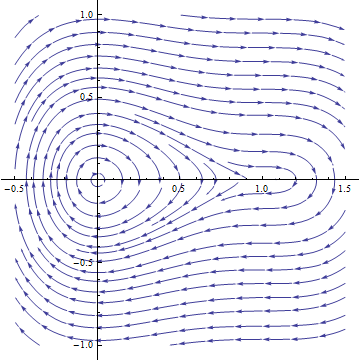
\includegraphics[scale=0.75]{./_Figures/S14Q6.png}
\end{center}

\subsubsection*{Solution to $6c$}
The ODE can be written as the system
\begin{equation}\label{s146aeq2}
\begin{aligned}
x' & = y\\
y' &= -x(1-x)^{2} - \abn{x}y.
\end{aligned}
\end{equation}
We have
$$yy' = -xy(1 - x) - |x|y^{2}$$
and hence
$$\bigg(\frac{y^{2}}{2}\bigg)' = -xx' + 2x^{2}x' - x^{3}x' - |x|y^{2} = -\bigg(\frac{x^{2}}{2}\bigg)' + \bigg(\frac{2}{3}x^{3}\bigg)' - \bigg(\frac{1}{4}x^{4}\bigg)' - |x|y^{2}.$$
Let
$$V(x, y) := \frac{y^{2}}{2} + \frac{x^{2}}{2} - \frac{2}{3}x^{3} + \frac{1}{4}x^{4}.$$
Then $V(0, 0) = 0$, $V(x, y) > 0$ for all $(x, y)$ sufficiently close to $(0, 0)$ and
$\dot{V}(x, y) = -|x|y^{2} < 0$ for all $(x, y) \neq (0, 0)$. Thus by Lyapunov theory, $(0, 0)$ is asymptotically stable.
\hfill\qed

\subsection*{Solution to Spring 2014, \#7}\label{s147}
\subsubsection*{Solution to $7a$}
We have
\begin{align*}
\dot{E}(\alpha) &= \int_{\Om}2(\Delta u + \alpha u)u\, dx\\
&= \int_{\Om}2u\delta u\, dx + 2\alpha\int_{\Om}u^{2}\, dx\\
&= -2\int_{\Om}\nabla u\cdot \nabla u\, dx + 2 \int_{\pr\Om}u\frac{\pr u}{\pr \nu}\, d\sigma + 2\alpha\int_{\Om}u^{2}\, dx\\
&= -2\int_{\Om}\nabla u \cdot \nabla u\, dx + 2 \int_{\pr\Om}u(-u)\, d\sigma + 2\alpha\int_{\Om}u^{2}\, dx
\end{align*}
where the third equality is because $u + \pr u/\pr \nu = 0$ on $\pr\Om$. Therefore as $E(r[u]) \leq E(\alpha)$ for all $\alpha \in \R$,
\begin{align*}
0 = \dot{E}(r[u]) = -2\int_{\Om}\abn{\nabla u}^{2}\, dx - 2\int_{\pr\Om}u^{2}\, d\sigma + 2r[u]\int_{\Om}u^{2}\, dx
\end{align*}
which implies
$$r[u] = \frac{\int_{\Om}\abn{\nabla u}^{2}\, dx + \int_{\pr\Om}u^{2}\, d\sigma}{\int_{\Om}u^{2}\, dx}.$$
\hfill\qed

\subsubsection*{Solution to $7b$}
Since $v$ minimizes the functional $r$ over all functions $w$ that satisfy $w(x) + \nabla w \cdot \nu = 0$ on $\pr\Om$, we must have
\begin{align}\label{s147eq1}
\frac{d}{d\vep}r[v + \vep w]\bigg|_{\vep = 0} = 0
\end{align}
for all $w$ such that $w + \nabla w \cdot \nu = 0$ on $\pr \Om$.
We compute
\begin{align*}
\bigg(\int_{\Om}&(v + \vep w)^{2}\, dx\bigg)^{2}\frac{d}{d\vep}r[v + \vep w]\\
&= \bigg(\int_{\Om}(v + \vep w)^{2}\, dx\bigg)\bigg(2\int_{\Om}\nabla(v + \vep w)\cdot \nabla w\, dx+ 2\int_{\pr\Om}(v + \vep w)w\, d\sigma\bigg)\\
&\quad\quad- \bigg(\int_{\Om}|\nabla(v + \vep w)|^{2}\, dx+ \int_{\pr\Om}(v + \vep w)^{2}\, d\sigma\bigg)\bigg(2\int_{\Om}(v + \vep w)w\, dx\bigg).
\end{align*}
Combining this with \eqref{s147eq1} yields
\begin{align*}
\bigg(\int_{\Om}v^{2}\, dx\bigg)\bigg(\int_{\Om}\nabla v \cdot \nabla w\, dx + \int_{\pr \Om}vw\, d\sigma\bigg) = \bigg(\int_{\Om}|\nabla v|^{2}\,dx + \int_{\pr\Om}v^{2}\, d\sigma\bigg)\bigg(\int_{\Om}vw\, d\sigma\bigg).
\end{align*}
Since both $v + \pr v/\pr \nu = 0$ and $w + \pr w/\pr \nu = 0$ on $\pr\Om$, integration by parts yields
$$\int_{\Om}\nabla v \cdot \nabla w\, dx = -\int_{\Om}w\Delta v\, dx - \int_{\pr\Om}wv\, d\sigma$$
and
\begin{align}\label{s147eq2}
\int_{\Om}\nabla v \cdot \nabla v\, dx = -\int_{\Om}v\Delta v\, dx - \int_{\pr\Om}v^{2}\, d\sigma.
\end{align}
Therefore
$$\bigg(\int_{\Om}v^{2}\, dx \bigg)\bigg(\int_{\Om}w\Delta v\, dx\bigg) = \bigg(\int_{\Om}v\Delta v\, dx\bigg)\bigg(\int_{\Om}vw\, dx\bigg).$$
Let $\alpha := \int_{\Om}v^{2}\, dx$ and $\beta := \int_{\Om}v\Delta v\, dx$. Then $\alpha\int_{\Om}w\Delta v\, dx = \beta\int_{\Om}vw\, dx$ and hence
$$\int_{\Om}w(\alpha \Delta v - \beta v)\, dx = 0$$
for all $w$ such that $w + \pr w/\pr\nu = 0$ on $\pr \Om$. This implies that $\alpha\Delta v - \beta v = 0$. That is,
\begin{align*}
\Delta v = \frac{\beta}{\alpha}v = \frac{\int_{\Om}v\Delta v\, dx}{\int_{\Om}v^{2}\, dx}v = -\bigg(\frac{\int_{\Om}\nabla v\cdot \nabla v\, dx + \int_{\pr\Om}v^{2}\, d\sigma}{\int_{\Om}v^{2}\, dx}\bigg)v = -r[v]v.
\end{align*}
\hfill\qed

\subsection*{Solution to Spring 2014, \#8}\label{s148}
We reserve $x_{0}$ to be used in the method of characteristics and will instead denote the $x_{0}$ in the problem statement as $\delta$.
For $\delta \in (0, 1)$, let
\begin{align*}
f(x) =
\begin{cases}
1 & \text{ if } 0 < x < \delta\\
0 & \text{ if } \delta < x < 1.
\end{cases}
\end{align*}
We follow the solution to Fall 2012, \#8. The characteristics of the PDE are given by $x = f(x_{0})t + x_{0}$ and crash immediately, so by the Rankine-Hugonito condition, the
shock curve $x = s(t)$ is given by
$$\dot{s}(t) = \frac{(1/2)\cdot 1^{2} - (1/2)\cdot 0^{2}}{1 - 0} = \frac{1}{2}$$
with initial condition $s(0) = \delta$. Therefore $s(t) = (1/2)t + \delta$ and so the shock is given by $x = \frac{1}{2}t +\delta$. We have the following picture.
\begin{center}
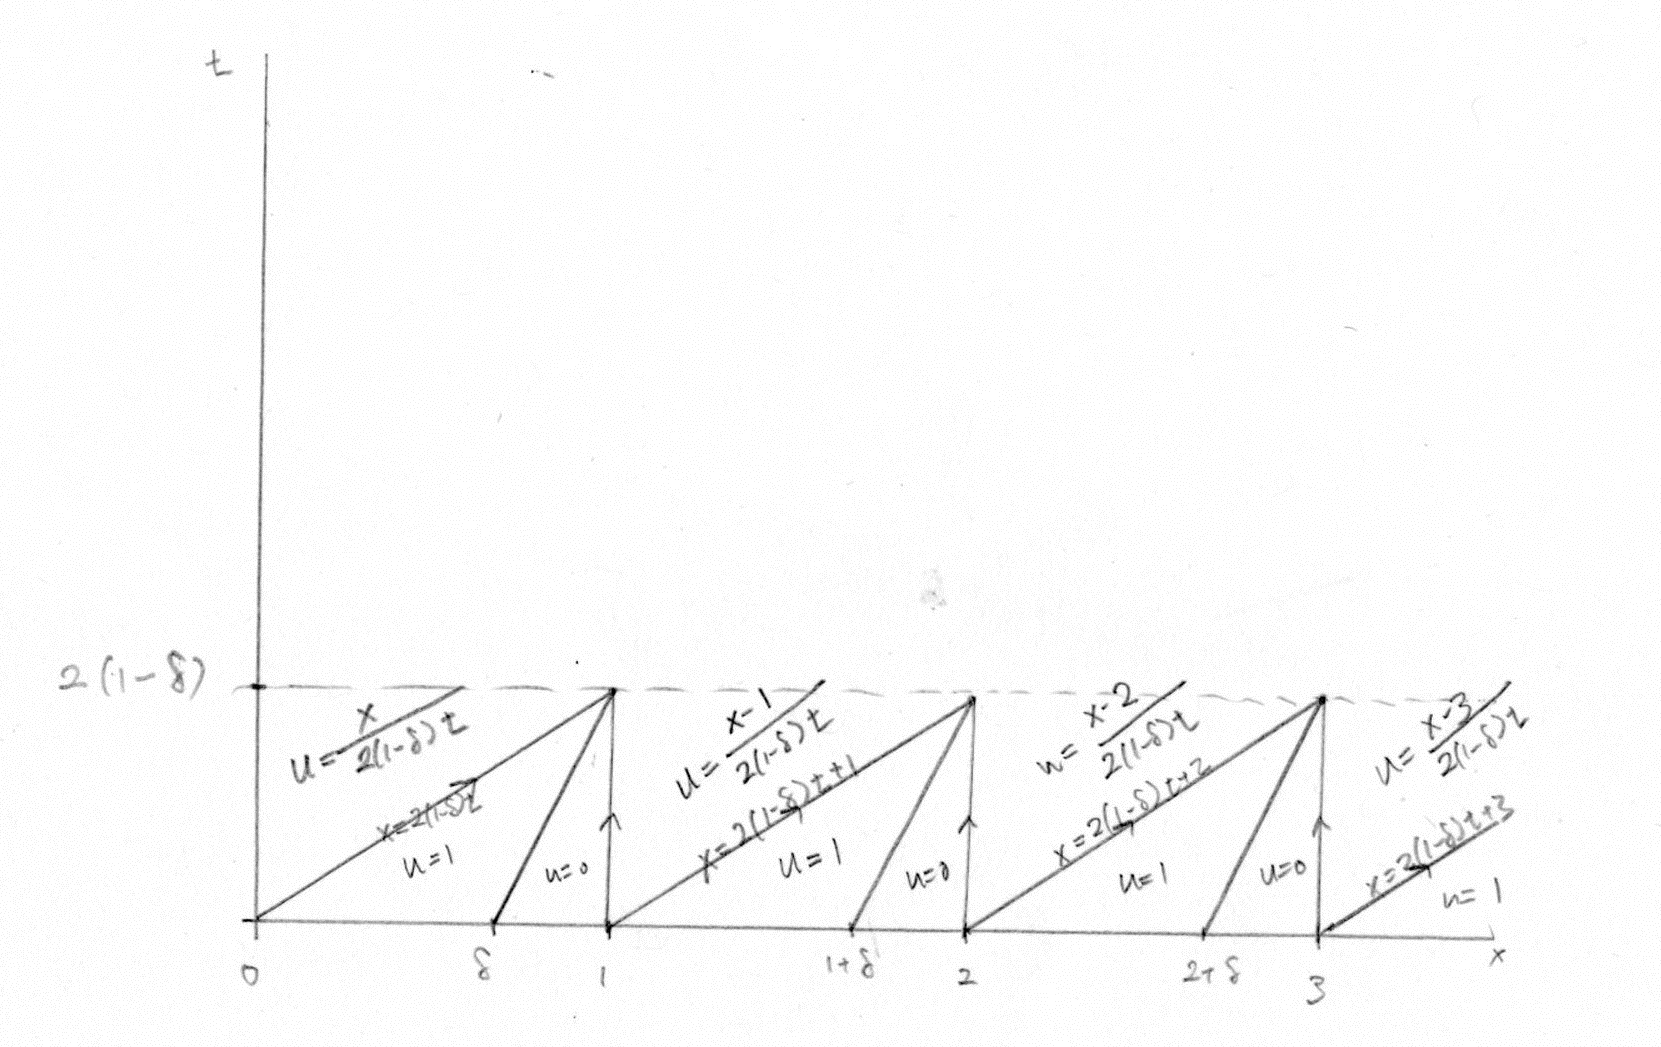
\includegraphics[scale = 0.35]{./_Figures/S14Q8a.png}
\end{center}
Thus we have another shock starting at the point $(x, t) = (k, 2(1 - \delta))$ which is given by
\begin{align*}
\dot{s}(t) = \frac{\frac{1}{2}\bigg(\frac{s(t) - (k - 1)}{2(1 - \delta)t}\bigg)^{2} - \frac{1}{2}\bigg(\frac{s(t) - k}{2(1 - \delta)t}\bigg)^{2}}{\frac{1}{2(1 - \delta)t}} = \frac{1}{2}\bigg(\frac{s(t) - k}{(1 - \delta)t} + \frac{1}{2(1 - \delta)t}\bigg) = \frac{s(t) - k + 1/2}{(1 - \delta)2t}
\end{align*}
with $s(2(1 - \delta)) = k$.
Solving this ODE via separation of variables and imposing the initial condition yields that the shock coming out of the point $(k, 2(1 - \delta))$ is given by
$$x= s(t) = \frac{1}{2}\bigg(\frac{t}{2(1 - \delta)}\bigg)^{\frac{1}{2(1 - \delta)}} + k - \frac{1}{2}.$$
Therefore the entropy solution is given by:
\begin{center}
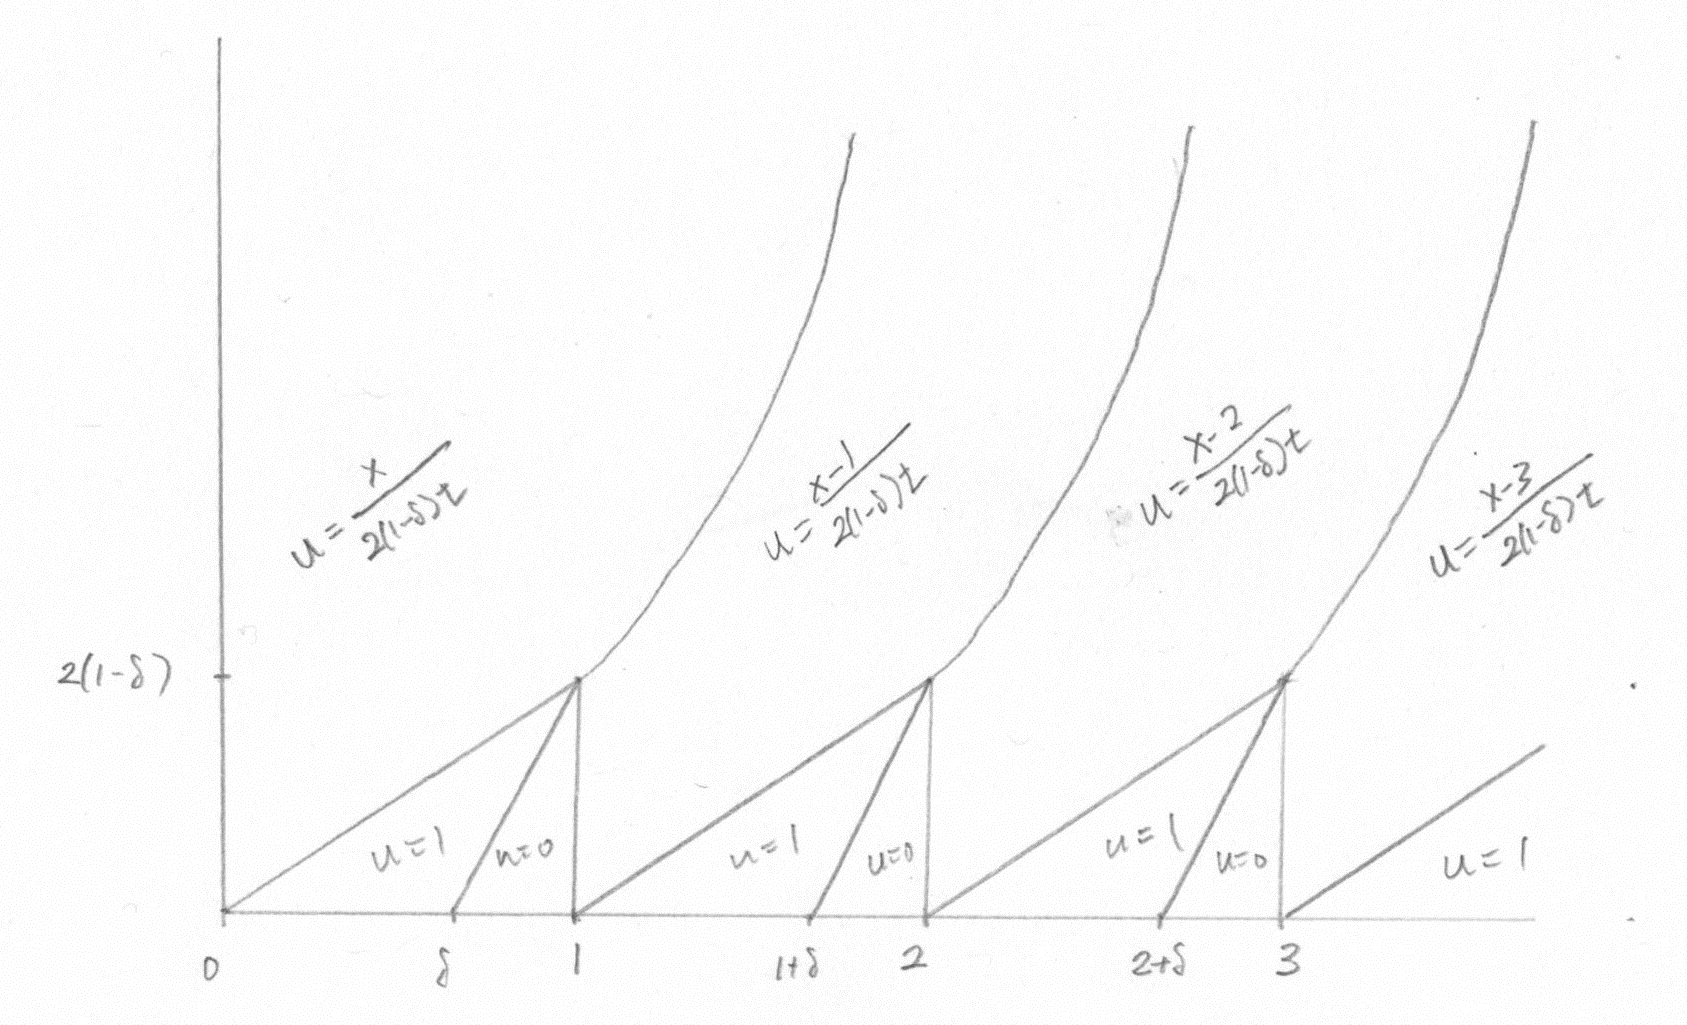
\includegraphics[scale=0.35]{./_Figures/S14Q8b.png}
\end{center}
\hfill\qed


\section{Fall 2013}\label{f13}
\subsection*{Solution to Fall 2013, \#1}
\label{F13Q1}

\subsubsection*{Solution to $1a$ and $1b$}

Since $\psi(x) = \frac{1}{2} (x^2-1)^2$, the ODE system is
$$ \left\{
\begin{array}{l}
x_t = v \\
v_t = -2x(x^2-1) - \alpha v
\end{array}
\right.
$$
Hence, the stationary points are $(-1,0)$, $(0,0)$, and $(1,0)$. Furthermore the Jacobian of the system is
$$ J(x,y) = \pmat{0}{1}{-6x^2 + 2}{-\alpha} $$
Then, we compute the eigenvalues and eigenvectors. For $J(0,0)$, the eigenvalues are $\frac{-\alpha \pm \sqrt{\alpha^2 + 8}}{2}$. For $J(\pm 1,0)$, we have that
the eigenvalues are $\frac{-\alpha \pm \sqrt{\alpha^2 - 16}}{2}$.
From the eigenvalues, $(0,0)$ will always be a saddle, while $(\pm 1, 0)$ depends on the value of $\alpha$.

If $0 < \alpha < 4$, then $(\pm 1, 0)$ are inward pointing spirals. Below is a phase plane plot for $\alpha = 1$.
\begin{center}
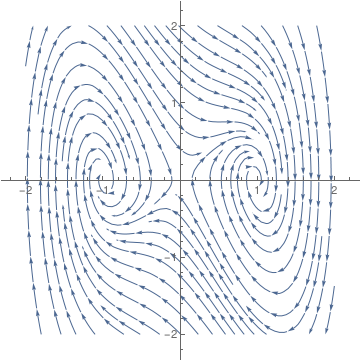
\includegraphics[scale=0.75]{./_Figures/f1311.png}
\end{center}

If $\alpha = 4$, then $(\pm 1, 0)$ are nodes (the eigenvalues for $J(\pm 1, 0)$ are repeated). Below is a phase plane plot for $\alpha = 4$.
\begin{center}
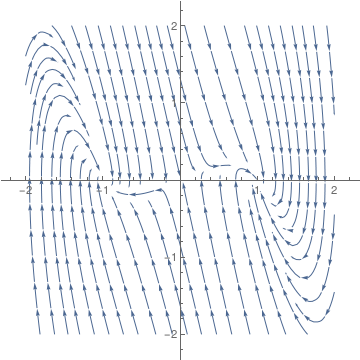
\includegraphics[scale=0.75]{./_Figures/f1312.png}
\end{center}

If $\alpha > 4$, then $(\pm 1, 0)$ are sinks. Below is a phase plane plot for $\alpha = 6$.
\begin{center}
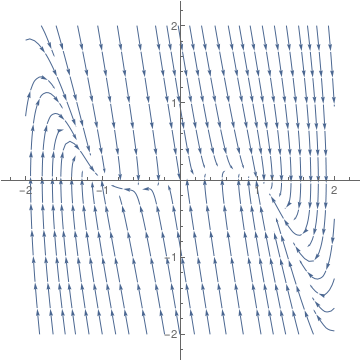
\includegraphics[scale=0.75]{./_Figures/f1313.png}
\end{center}

\subsubsection*{Solution to $1c$}

To how $H$ is non-increasing with time, we take a time derivative. Same as in parts (a) and (b), we assume $\alpha < 0$.
$$ \dot{H}(x,v) = v \dot{v} + \psi'(x) \dot{x} = v(-2x(x^2-1)-\alpha v) + 2xv(x^2-1) = -\alpha v^2 < 0 $$
Hence, $H$ is non-increasing with time. \hfill \qed


\subsection*{Solution to Fall 2013, \#2}
\label{F13Q2}

\subsubsection*{Solution to $2a$}
	
First, observe that, with the given choice of $f$, $E$ can be succinctly written as
\begin{equation}
	\label{F13Q2one}
	E(u) = \frac{1}{2} \int_{\Omega} \abs{\del u}^2 + gu \,dx + \frac{1}{2} \int_{\d \Omega} u^2 \, dS(x)
\end{equation}
Now, suppose $u$ minimizes \eqref{F13Q2one}, and let $v \in H^1(\Omega)$. We compute
$$ \frac{1}{\epsilon} \left(E(u+\epsilon v) - E(u) \right) = \int_{\Omega} \del u \cdot \del v + \epsilon v^2 + gv \,dx + \int_{\d \Omega} u v + \epsilon v^2 \, dS(x) $$
Since $u$ is a minimizer of $E$, sending $\epsilon \to 0$ yields
$$ \int_{\Omega} \del u \cdot \del v + gv \,dx + \int_{\d \Omega} u v \, dS(x) = 0 \quad \Leftrightarrow \quad \int_{\Omega} \del u \cdot \del v \, dx + \int_{\d \Omega} u v \, dS(x) = - \int_{\Omega} gv \, dx $$
Define the bilinear form $B : H^1(\Omega) \times H^1(\Omega) \to \R$ as
$$ B[u,v] = \int_{\Omega} \del u \cdot \del v \, dx + \int_{\d \Omega} uv \, dS(x) $$
and the function $F : H^1(\Omega) \to \R$ as
$$ F(v) = -\int_{\Omega} gv \, dx $$
Assuming $g \in L^2(\Omega)$, it's straightforward to check that both $B$ and $F$ are bounded:
\begin{align*}
	|B[u,v]| &\leq \nm{\del u}_{L^2(\Omega)} \nm{\del v}_{L^2(\Omega)} + \nm{u}_{L^2(\d \Omega)} \nm{v}_{L^2(\d \Omega)} \\
	&\leq 2 \nm{u}_{H^1(\Omega)} \nm{v}_{H^1(\Omega)}
\end{align*}
and
$$ |F(v)| \leq \nm{g}_{L^2(\Omega)} \nm{v}_{L^2(\Omega)} \leq C \nm{v}_{H^1(\Omega)} $$
(Note: In order to show $B$ is bounded, we invoked the Trace Theorem, which states $\nm{u}_{L^2(\d \Omega)} \leq \nm{u}_{H^1(\Omega)}$.) Furthermore, $B$ is symmetric and satisfies the property $B[u,u] \geq 0$ for all $u \in H^1(\Omega)$ and $B[u,u] = 0$ if $u \equiv 0$. If $B[u,u] = 0$, then $\del u \equiv 0$ in $\Omega$ and $u \equiv 0$ on $\d \Omega$. The condition on the derivative implies $u$ must be constant, and pairing this with the condition on the boundary implies $u \equiv 0$. Thus, $B$ defines an inner product on $H^1(\Omega)$, and by the Riesz Representation Theorem, there exists a unique $u \in H^1(\Omega)$ such that
\begin{equation}
\label{F13Q2two}
	B[u,v] = F(v) \quad \forall v \in H^1(\Omega)
\end{equation}

Now, we reverse the work we've done to obtain the result. Define $B$ and $F$ as stated above, and observe that there exists a unique $u \in H^1(\Omega)$ such that \eqref{F13Q2two} holds. Because of how we defined $B$ and $F$, $u$ must be the unique critical point of $E$. Finally, since $E$ is convex, $u$ must minimize $E$. Therefore, $E$ has a unique minimizer in $H^1(\Omega)$.  \hfill \qed

\subsubsection*{Solution to $2b$}

Recall from our work above that the minimizer $u$ of $E$ must satisfy
$$ \int_{\Omega} \del u \cdot \del v + gv \,dx + \int_{\d \Omega} u v \, dS(x) = 0 $$
for all $v \in H^1(\Omega)$. Applying integration by parts to the first term above yields
$$ \int_{\Omega} -\Delta u v \, dx + \int_{\d \Omega} \frac{\d u}{\d \nu} v \, dS(x) + \int_{\Omega} gv \, dx + \int_{\d \Omega} uv \, dS(x) = 0 $$
Since this holds for all $v \in H^1(\Omega)$, we obtain the following differential equation and boundary condition for the minimizer of $E$:
$$ \Delta u = g \quad \text{in} \,\, \Omega $$
$$ \frac{\d u}{\d \nu} + u = 0 \quad \text{on} \,\, \d \Omega $$
\hfill \qed

\subsubsection*{Solution to Fall 2013, \#2$(a)$ with Lax-Milgram}
Let
\begin{align*}
B[u, v] := \int_{\Om}\nabla u \cdot \nabla v\, dx + \int_{\pr \Om}uv\, d\sigma \quad \text{ and } \quad \psi(v) := \int_{\Om} -g v\, dx.
\end{align*}
Note
$$|B[u, v]| \leq \nms{\nabla u}_{L^{2}(\Om)}\nms{\nabla v}_{L^{2}(\Om)} + \|u\|_{L^{2}(\pr \Om)}\|v\|_{L^{2}(\pr \Om)} \leq C\|u\|_{H^{1}(\Om)}\|v\|_{H^{1}(\Om)}$$
by the boundedness of the trace operator (strictly speaking, we should really be writing $\|Tu\|_{L^{2}(\pr \Om)}$ instead of $\|u\|_{L^{2}(\pr \Om)}$ where
$T: H^{1}(\Om) \rightarrow L^{2}(\pr \Om)$ where $T$ is the trace operator). As $g \in L^{2}$,
$$|\psi(v)| \leq \|g\|_{L^{2}(\Om)}\|v\|_{L^{2}(\Om)} \leq \|g\|_{L^{2}(\Om)}\|v\|_{H^{1}(\Om)}$$
and so $\psi$ is a bounded linear functional on $H^{1}(\Om)$.

To prove existence of a weak solution, it now remains to show that $B[u, v]$ is coercive (that is, there exists a $\beta$ such that
$\beta \|u\|_{H^{1}}^{2} \leq B[u, u]$ for all $u \in H^{1}$). Suppose $B$ was not coercive, then there exists
$\{u_{n}\}$ such that $\nms{u_{n}}_{H^{1}(\Om)} = 1$ and $B[u_{n}, u_{n}] \rightarrow 0$ as $n \rightarrow \infty$.
By weak compactness, there exists a subsequence $\{u_{n_{k}}\} \subset \{u_{n}\}$ and a $u \in H^{1}(\Om)$ such that
$u_{n_{k}} \rightharpoonup u$ as $k \rightarrow \infty$ in $H^{1}(\Om)$. Since a weakly convergent sequence is bounded and by
Rellich-Kondrachov, $H^{1}(\Om)$ embeds compactly into $L^{2}(\Om)$, we have a further subsequence such that
$u_{n_{k_{j}}} \rightarrow u$ as $n_{k_{j}} \rightarrow \infty$ in $L^{2}(\Om)$.

We have
\begin{align}\label{altf132eq1}
B[u_{n_{k_{j}}}, u_{n_{k_{j}}}] = \int_{\Om}|\nabla u_{n_{k_{j}}}|^{2}\, dx + \int_{\pr \Om}u_{n_{k_{j}}}^{2}\, d\sigma \rightarrow 0.
\end{align}
Thus
$$\int_{\Om}|\nabla u_{n_{k_{j}}}|^{2}\, dx \rightarrow 0$$
as $n_{k_{j}} \rightarrow \infty$.
Since $u_{n_{k}} \rightharpoonup u$ in $H^{1}(\Om)$,
\begin{align}\label{altf132}
\int_{\Om}(u_{n_{k_{j}}} - u)v\, dx + \int_{\Om}\nabla(u_{n_{k_{j}}} - u)\cdot \nabla v\, dx \rightarrow 0
\end{align}
for all $v \in H^{1}(\Om)$. Indeed, for each $v \in H^{1}(\Om)$, let $L_{v} : H^{1}(\Om) \rightarrow \R$ be defined by
$$L_{v}(u) := \int_{\Om}uv\, dx + \int_{\Om}\nabla u \cdot \nabla v\, dx.$$ Since $u_{n_{k}}\rightharpoonup u$, $L_{v}(u_{n_{k}}) \rightarrow L_{v}(u)$ which
proves \eqref{altf132}.
Then as $u_{n_{k_{j}}} \rightarrow u$ in $L^{2}(\Om)$, taking $v = u$ in \eqref{altf132} yields
$$\int_{\Om}|\nabla u|^{2}\, dx = \lim_{n_{k_{j}} \rightarrow \infty}\int_{\Om}\nabla u_{n_{k_{j}}} \cdot \nabla u = 0.$$
Therefore $\nms{u}_{H^{1}(\Om)} = \nms{u}_{L^{2}(\Om)}$. Then
$$\nms{u}_{L^{2}(\Om)} = \lim_{n_{k_{j}} \rightarrow \infty}\nms{u_{n_{k_{j}}}}_{L^{2}(\Om)} = 1.$$
Since $\int_{\Om}|\nabla u|^{2}\, dx = 0$, $u$ is constant on $\Om$. Since $\|u\|_{L^{2}(\Om)} = 1$, $u = c \neq 0$.

However, by \eqref{altf132eq1}
$$\int_{\pr \Om}u^{2}\, d\sigma = \lim_{n_{k_{j}} \rightarrow \infty}\int_{\pr \Om}u_{n_{k_{j}}}^{2}\, d\sigma = 0,$$
(here we are once again abusing notation and we should be writing $Tu$ and $Tu_{n_{k_{j}}}$ instead, the above equation is essentially
the fact that trace is a continuous linear operator) and hence $u = 0$ on $\pr \Om$, a contradiction since $u = c \neq 0$ in $\Om$.
Thus $B$ is coercive. Thus by Lax-Milgram, there exists a unique $\wt{u} \in H^{1}(\Om)$ such that $B[\wt{u}, v] = \psi(v)$ for all $v \in H^{1}(\Om)$.
\hfill\qed

\subsection*{Solution to Fall 2013, \#3}
\label{F13Q3}

We solve this using method of characteristics. Because the PDE is quasilinear, we only need to solve the following ODEs to obtain our solution:
\begin{align}
\label{F13Q3Eqt} &\dot t(s) = 1, \quad t(0) = 0 \\
\label{F13Q3Eqx} &\dot x(s) = f'(z(s)), \quad x(0) = x_0 \\
\label{F13Q3Eqz} &\dot z(s) = 0, \quad z(0) = \phi(x_0) = -x_0 \\
\end{align}
Solving \eqref{F13Q3Eqt} and \eqref{F13Q3Eqz} yield
$$ t(s) = s, \quad z(s) = -x_0 $$
respectively. Then, solving \eqref{F13Q3Eqx} yields
$$ x(s) = f'(-x_0)t + x_0 $$
This implies
$$ u(x,t) = -x_0, \quad \text{where} \,\,\, x = f'(-x_0)t + x_0 $$
Taking a partial derivative of $u$ with respect to $x$ yields $u_x = -\frac{\d x_0}{\d x}$. Next, we compute
\begin{align*}
\frac{\d}{\d x} \left[ x = f'(-x_0)t + x_0 \right] \quad &\implies \quad 1 = -f''(-x_0)t \frac{\d x_0}{\d x} + \frac{\d x_0}{\d x} \\
&\implies \quad \frac{\d x_0}{\d x} = \frac{1}{1 - f''(-x_0)t}
\end{align*}
Thus,
$$ |u_x(x,t)| = \frac{1}{|1-f''(-x_0)t|} $$
Since $f''(u) \geq \theta > 0$ for all $u$, we know that, by the time $t = 1/\theta$, the expression $1-f''(-x_0)t$ will have already equaled 0. Therefore, $|u_x| \to \infty$ in finite time. \hfill \qed



\subsection*{Solution to Fall 2013, \#4}
\label{F13Q4}

We think there is a typographical error in the problem statement. Specifically, we think the PDE should read
$$ u_{tt} + c^2 u_{xxxx} + au_t = 0 $$
(a plus sign instead of a minus sign between the first two terms). Our solution reflects this change.

\subsubsection*{Solution to $4a$}

If this is indeed the intended PDE, define the energy
$$ E(t) := \frac{1}{2} \int_{\R} u_t^2 + c^2 u_{xx}^2 \, dx $$
Then,
$$ \dot{E}(t) = \int_{\R} u_t u_{tt} + c^2 u_{xx} u_{xxt} \, dx $$
Since we're assuming solutions have compact support, two application of integration by parts yields
$$ \dot{E}(t) = \int_{\R} u_t u_{tt} + c^2 u_{xxxx}u_t \, dx = \int_{\R} -a u_t^2 \, dx \leq 0 $$
Hence, the energy is non-increasing with time. \hfill \qed

\subsubsection*{Solution to $4b$}

Let $u$ and $v$ be solutions with compactly supported initial data, and consider $ w:= u-v$. Observe that $w$ satisfies
$$ \left\{
\begin{array}{lll}
w_{tt} + c^2 w_{xxxx} + aw_t = 0 \\
w(x,0) = 0 \\
w_t(x,0) = 0
\end{array}
\right. $$
Furthermore, since both $u$ and $v$ are compactly supported, $w$ is as well (see remark below). Thus, defining the energy as
$$ E(t) := \frac{1}{2} \int_{\R} w_t^2 + c^2 w_{xx}^2 \, dx $$
and using the same argument as in $4a$ yields $\dot{E}(t) \leq 0$. Furthermore, observe that $E(0) = 0$. Finally, because $E(t) \geq 0$ for all time, we must have that $E(t) \equiv 0$ for all time. This implies $w_t \equiv 0$ and $w_{xx} \equiv 0$. This implies that $w(x,t) = f(x)$, a function dependent only on $x$. Since $w_{xx} \equiv 0$, we know $f''(x) = 0$, implying that $w(x,t) = ax+b$ for some $a, b \in \R$. Then, $w(x,0) = 0$ implies $b=0$. Now, $0 = w(x,0) = ax$ implies $a = 0$, too. We've shown $w \equiv 0$, and therefore, solutions are unique. \hfill \qed

\begin{rem}
In the solution, we stated without proof that solutions with compactly supported initial data must be compactly supported. This can be shown by following Evans' proof of the domain of dependence for the wave equation (pg. 84, 2nd edition), but with the use of the energy defined for this problem.
\end{rem}


\subsection*{Solution to Fall 2013, \#5}
\label{F13Q5}

First, let's assume $4aT < 1$. Then, there exists $\delta > 0$ and $\gamma > 0$ such that
$$ 4a(T+\delta) < 1 \quad \text{and} \quad \frac{1}{4(T+\delta)} = a + \gamma $$
Fix an arbitrary $y \in \R$ and $\epsilon > 0$. Let
$$ v(x,t) := u(x,t) - \frac{\epsilon}{(T+\delta -t)^{1/2}} e^{\frac{(x-y)^2}{4(T+\delta - t)}} $$
Then, observe that
\begin{align*}
\frac{\d}{\d t} (T-\delta - t)^{-1/2} e^{\frac{(x-y)^2}{4(T+\delta - t)}} &= \left[ \frac{1}{2} \frac{1}{(T+\delta -t)^{3/2}} + \frac{1}{4} \frac{(x-y)^2}{(T+\delta - t)^{5/2}}\right]  e^{\frac{(x-y)^2}{4(T+\delta - t)}} \\
&= \frac{\d^2}{\d x^2} (T-\delta - t)^{-1/2} e^{\frac{(x-y)^2}{4(T+\delta - t)}}
\end{align*}
so we have $v_t - v_{xx} = 0$ in $\R \times (0,T]$. Let $r > 0$ be sufficiently large to be chosen later and let $U := B_r(y)$, $U_T := B_r(y) \times (0,T]$. Then, by the maximum principle for the heat equation
\begin{equation}
\label{f135max}
\max_{\overline{U_T}} v = \max_{\Gamma_T} v
\end{equation}
where $\Gamma_T := \overline{U_T} \bs U_T$.
Note that
$$ v(x,0) = u(x,0) - \frac{\epsilon}{(T+\delta)^{1/2}} e^{\frac{(x-y)^2}{4(T+\delta)}} \leq u(x,0) = 0 $$
and for $x$ such that $|x-y| = r$, we have
\begin{align*}
v(x,t) &= u(x,t) - \frac{\epsilon}{(T+\delta -t)^{1/2}} e^{\frac{(x-y)^2}{4(T+\delta - t)}} \\
&\leq Ce^{ax^2} - \frac{\epsilon}{(T+\delta -t)^{1/2}} e^{\frac{r^2}{4(T+\delta - t)}} \\
&\leq Ce^{ax^2} - \frac{\epsilon}{(T+\delta)^{1/2}} e^{\frac{(x-y)^2}{4(T+\delta)}} \\
&\leq Ce^{a(|y|+r)^2} - \epsilon (4(a+\gamma))^{1/2} e^{(a+\gamma)r^2} \leq 0
\end{align*}
if $r$ is sufficiently large. Thus, by \eqref{f135max} and the arbitrariness of $y$, $v(y,t) \leq 0$ for all $0 \leq t \leq T$ and $y \in \R^n$. Letting $\epsilon \to 0$ shows that $u(x,t) \leq 0$ for all $x \in \R^n$, $0 \leq t \leq T$. Replacing $u$ with $-u$ shows that $u(x,t) = 0$ for all $x \in \R^n$, $0 \leq t \leq T$ if $4aT < 1$.

If $4aT \geq 1$, then we repeatedly apply the result on the time intervals $[0,T_1], [T_1,2T_1], \dots$ for $T_1 = \frac{1}{8a}$. \hfill \qed



\subsection*{Solution to Fall 2013, \#6}
\label{F13Q6}

Suppose $u$ is a solution of the given PDE. As the equation looks like a nonlinear version
of the transport equation, let $z(s) := u(x - s, t + s)$. Then
$$\dot{z}(s) = u_{x}(x - s, t + s)(-1) + u_{t}(x - s, t + s) = -u^{2}(x - s, t + s)$$
and hence
$$u(x, t) - \psi(x + t) = z(0) - z(-t) = \int_{-t}^{0}-u^{2}(x - s, t + s)\, ds = \int_{0}^{t}-u^{2}(x - s + t, s)\, ds.$$
Then
$$u(x, t) = \psi(x + t) - \int_{0}^{t}u^{2}(x - s + t, s)\, ds.$$
Therefore a solution to the given PDE is a fixed point of the operator
$$F(\vp)(x, t) := \psi(x + t) - \int_{0}^{t}\vp^{2}(x - s + t, s)\, ds$$
where $\vp \in \textrm{BC}(\R^{2} \rightarrow \R)$, the bounded continuous functions from $\R^{2} \rightarrow \R$
which is a complete metric space under the sup norm $\nms{\cdot}_{\infty}$.
Since $\psi$ is smooth with compact support, $\nms{\psi}_{\infty} = \sup_{x \in \R}\abn{\psi(x)} < \infty$.
Let $T$ be such that $T\nms{\psi}_{\infty} \leq 1/100$. Then
\begin{align}
\label{F13Q6one}
\nms{F(\vp)}_{\infty} \leq \nms{\psi}_{\infty} + T\nms{\vp}_{\infty}^{2} \leq \nms{\psi}_{\infty} + \frac{1}{100\nms{\psi}_{\infty}}\nms{\vp}_{\infty}^{2}.
\end{align}

Let $V := \{\vp \in \textrm{BC}(\R^{2} \rightarrow \R): \|\vp\|_{\infty} \leq 2\|\psi\|_{\infty}\}$.
Since $V$ is a closed subset of $\textrm{BC}(\R^{2} \rightarrow \R)$, $V$ is complete.
We will show that
$F: V \rightarrow V$ and that $F$ is a contraction on $V$. Explicitly, we will show that $F(\vp) \in V$ for all $\vp \in V$
and for any $\vp, \phi \in V$, $\|F(\vp) - F(\phi)\|_{\infty} \leq \alpha \|\vp - \phi\|_{\infty}$ for some $\alpha < 1$.

We first show that $F(\vp) \in V$ for all $\vp \in V$. By \eqref{F13Q6one}, we have
\begin{align*}
\|F(\vp)\|_{\infty} \leq \|\psi\|_{\infty} + \frac{1}{100\nms{\psi}_{\infty}}4\|\psi\|_{\infty}^{2} < 2\|\psi\|_{\infty}
\end{align*}
and hence $F(\vp) \in V$. Next,
\begin{align*}
\|F(\vp) - F(\phi)\|_{\infty} &= \bigg\|\int_{0}^{t}\phi(x - s + t, s)^{2} - \vp(x - s + t, s)^{2}\, ds\bigg\|_{\infty}\\
&\leq 4T\|\psi\|_{\infty}\|\phi - \vp\|_{\infty} \leq \frac{1}{25}\|\phi - \vp\|_{\infty}.
\end{align*}

Thus $F$ is a contraction on $V$. Therefore there exists a unique fixed point in $V$. Since fixed points of
$F$ are solutions to the PDE, there exists a unique solution to the PDE if $T$ is chosen sufficiently small. \hfill\qed

\subsection*{Solution to Fall 2013, \#7}
\label{F13Q7}

Based on the information given in the problem, we don't know whether or not $u$ is continuous at the origin. If it is, we will show that $u$ is harmonic in all of $\R^3$, and if not, we will show that $u$ can be harmonically extended to all of $\R^3$.

Let $v$ satisfy the following conditions
$$ \left\{
\begin{array}{ll}
\Delta v = 0 & \text{in} \,\, B_1(0) \\
v = u & \text{on} \,\, \d B_1(0)
\end{array} \right. $$
where $u$ is the function defined in the problem statement. Let $w := u-v$, and observe that $w$ satisfies
$$ \left\{
\begin{array}{ll}
\Delta w = 0 & \text{in} \,\, B_1(0) \bs \sq{0} \\
w = 0 & \text{on} \,\, \d B_1(0)
\end{array} \right. $$
Since $u = o\left(\frac{1}{|x|}\right)$ and $v$ is bounded in $\overline{B_1(0)}$, we have
$$ \lim_{x \to 0} \frac{w(x)}{\frac{1}{|x|}} = 0 $$
Hence, for all $\epsilon > 0$, there exists $\delta > 0$ such that
$$ w(x) \leq \frac{\epsilon}{|x|} \quad \Leftrightarrow \quad  w(x) - \frac{\epsilon}{|x|} \leq 0 $$
for all $0 < |x| \leq \delta$, or in other words, for all $x \in \overline{B_{\delta}(0)} \bs \sq{0}$. Now, observe that $w(x) - \frac{\epsilon}{|x|}$ is harmonic on $\R^3 \bs \sq{0}$ and
$$w(x) - \frac{\epsilon}{|x|} = -\epsilon \leq 0$$
for all $x \in \d B_1(0)$. Hence, by the maximum principle for harmonic functions, $w(x) - \frac{\epsilon}{|x|} \leq 0$ for all $x \in \overline{B_1(0)} \bs B_{\delta}(0)$. Putting everything together yields
$$ w(x) - \frac{\epsilon}{|x|} \leq 0 \quad \Leftrightarrow \quad w \leq \frac{\epsilon}{|x|} $$
for all $x \in \overline{B_1(0)} \bs \sq{0}$. Since $\epsilon$ was chosen arbitrarily, sending $\epsilon \to 0$ yields $w(x) \leq 0$, and hence, $u(x) \leq v(x)$, for all $x \in \overline{B_1(0)} \bs \sq{0}$. Interchanging the roles of $u$ and $v$ yields $u(x) = v(x)$ for all $x \in \overline{B_1(0)} \bs \sq{0}$.

If $u$ is not defined at $x=0$, then setting $u(0) := v(0)$ shows that we can extend $u$ to be harmonic on all of $\R^3$. If $u$ is defined at $x=0$, then the work above shows that $u(0) = v(0)$, and since $v$ is harmonic in $B_1(0)$, $u$ will also be harmonic in $B_1(0)$.  \hfill \qed



\subsection*{Solution to Fall 2013, \#8}
\label{F13Q8}

\subsubsection*{Solution to $8a$}

There are two ways to argue this --- integration by parts or Hopf's lemma, both of which will be explained.

Using integration by parts,
$$ 0 = \int_H u \Delta u \, dx = -\int_H |\nabla u|^2 \, dx $$
Note that the boundary terms vanish because $u_y(x,0) = 0$ for all $x \in \R$, and $u \to 0$ as $x^2 + y^2 \to \infty$. Hence, $\nabla u \equiv 0$ in the upper half-plane, implying that $u$ is constant. Finally, because $u \to 0$ as $x^2 + y^2 \to \infty$, we must have $u \equiv 0$. \hfill \qed

\vspace{0.2cm}

Define $H := \{(x,y) \in \R^2 \, : \, y \geq 0 \}$. To use Hopf's lemma, we first fix $\epsilon > 0$ and pick $R > 0$ such that $u \leq \epsilon$ on $\d B_R(0) \cap H$. Observe that $\Delta u = 0$ in $B_R(0) \cap H$, so by the maximum principle for harmonic functions, the maximum of $u$ must occur $\d (B_R(0) \cap H)$. Note that $\d (B_R(0) \cap H)$ consists of the following two pieces:
$$\d B_R(0) \cap H, \quad \text{and} \quad \{ (x,0) \in \R^2 \, : \, |x| < R \}$$
Suppose the maximum of $u$ occurs on the latter set, and furthermore, suppose it is a strict maximum. If it weren't a strict maximum, then by the strong maximum principle, $u$ will be constant in $B_R(0) \cap H$, implying that $u \leq \epsilon$ in $B_R(0) \cap H$. Because the maximum is assumed to be strict, Hopf's lemma states that $u_y > 0$ at the maximum, which contradicts the boundary condition. Thus, a strict maximum cannot occur on $\{(x,0) \, : \, |x| < R \}$. If the maximum occurs on $\d B_R(0) \cap H$, then we immediately have $u \leq \epsilon$ in $B_R(0) \cap H$. Hence, regardless, we have shown $u \leq \epsilon$ in $B_R(0) \cap H$. Since this holds for all $\epsilon > 0$ (and we may always choose $R>0$ so that this argument holds), sending $\epsilon \to 0$ allows us to send $R \to \infty$, implying that $u \leq 0$ in $H^0$, the interior of $H$. Running through the same argument with $-u$ instead of $u$ yields $u \geq 0$, so we have shown $u \equiv 0$ in the interior of $H$. \hfill \qed

\subsubsection*{Solution to $8b$}

Taking a Fourier transform in the $x$ variable of the PDE yields
$$
\left\{
\begin{array}{l}
-4\pi^2 \xi^2 \hat{u} (\xi, y) + \hat{u}_{yy}(\xi,y) = 0 \\
\hat{u}_y(\xi,0) = \hat{f}(\xi)
\end{array}
\right.
$$
Note that, since $f$ is compactly supported, $\hat{f} \in S(\R)$ ($\hat{f}$ is a Schwartz function). Solving the above PDE yields
$$ \hat{u}(\xi,y) = A e^{-2\pi |\xi| y} + B e^{2 \pi |\xi| y} $$
for some $A$ and $B$. Since we only need to show there exists \emph{a} solution that tends to 0 as $x^2 + y^2 \to \infty$, we'll let $B=0$. Now, applying $\hat{u}_y(\xi,0) = \hat{f}(\xi)$ yields
$$ \hat{u}(\xi,y) = -\frac{\hat{f}(\xi)}{2 \pi |\xi|} e^{-2 \pi |\xi| y} $$
Thus
\begin{align*}
u(x,y) &= \int_{\R} -\frac{\hat{f}(\xi)}{2 \pi |\xi|} e^{-2 \pi |\xi| y} e^{2 \pi i \xi x} \, d\xi \\
&= \int_{-\infty}^0 \frac{\hat{f}(\xi)}{2 \pi \xi} e^{2 \pi \xi y} e^{2 \pi i \xi x} \, d\xi + \int_0^{\infty} -\frac{\hat{f}(\xi)}{2 \pi \xi} e^{-2 \pi \xi y} e^{2 \pi i \xi x} \, d\xi \\
&= \int_{-\infty}^0 \frac{\hat{f}(\xi)}{2 \pi \xi} e^{2 \pi i \xi (x - iy)} \, d\xi + \int_0^{\infty} -\frac{\hat{f}(\xi)}{2 \pi \xi} e^{2 \pi i \xi (x + iy)} \, d\xi \\
&= \int_{-\infty}^0 \frac{\hat{f}(\xi)}{2 \pi \xi} \frac{1}{2 \pi i (x-iy)} \frac{d}{d \xi} e^{2 \pi i \xi (x - iy)} \, d\xi + \int_0^{\infty} -\frac{\hat{f}(\xi)}{2 \pi \xi} \frac{1}{2 \pi i(x+iy)} \frac{d}{d \xi} e^{2 \pi i \xi(x+iy)} \, d\xi
\end{align*}
Applying integration by parts yields
\begin{align*}
 u(x,y) =  \frac{1}{2 \pi i (x-iy)}& \left[\frac{\hat{f}(\xi)}{2 \pi \xi} e^{2 \pi i \xi (x - iy)}  \bigg|_{-\infty}^0 - \int_{-\infty}^0 \frac{d}{d \xi} \left( \frac{\hat{f}(\xi)}{2 \pi \xi} \right) e^{2 \pi i \xi (x - iy)} \, d\xi \right] + \\
&\frac{1}{2 \pi i (x+iy)} \left[-\frac{\hat{f}(\xi)}{2 \pi \xi} e^{2 \pi i \xi (x + iy)}  \bigg|_{0}^{\infty} + \int_{0}^{\infty} \frac{d}{d \xi} \left( \frac{\hat{f}(\xi)}{2 \pi \xi} \right) e^{2 \pi i \xi (x + iy)} \, d\xi \right]
\end{align*}
Because $\int_{-\infty}^{\infty} f(x) \, dx = 0$, we have $\hat{f}(0) = 0$. Thus,
$$ \frac{\hat{f}(\xi)}{2 \pi \xi} e^{2 \pi i \xi (x - iy)}  \bigg|_{-\infty}^0 = \lim_{\xi \to 0^-}\frac{\hat{f}(\xi)}{2 \pi \xi} e^{2 \pi i \xi (x - iy)}  = 0$$
and similarly,
$$ -\frac{\hat{f}(\xi)}{2 \pi \xi} e^{2 \pi i \xi (x + iy)}  \bigg|_{0}^{\infty} = 0 $$
Furthermore, because $\hat{f} \in S(\R)$, the integrals in the expression for $u$ converge. Hence,
$$ u(x,y) = \frac{C}{2\pi i(x-iy)} + \frac{\tilde{C}}{2 \pi i(x+iy)} $$
for constants $C$ and $\tilde{C}$. Finally,
$$ |u(x,y)| \leq \frac{C'}{2 \pi \sqrt{x^2 + y^2}} $$
where $C' \geq \max\{ |C|, |\tilde{C}|\}$. Therefore, we have $u \to 0$ as $x^2 + y^2 \to 0$. \hfill \qed


\section{Spring 2013}\label{s13}
\subsection*{Solution to Spring 2013, \#1}\label{s131}
Taking the Fourier transform, we have $\wh{u}_{t} = t^{2}(-4\pi^{2}|\xi|^{2})\wh{u}.$
Thus
$\wh{u}(\xi, t) = \wh{g}(\xi)e^{-\frac{4}{3}\pi^{2}|\xi|^{2}t^{3}}.$
Therefore
$u(x, t) = g(x) \ast [e^{-\frac{4}{3}\pi^{2}|\xi|^{2}t^{3}}]^{v}$.
Note that $e^{-\frac{4}{3}\pi^{2}|\xi|^{2}t^{3}}$ is a Schwarz function in $\xi$. Since the Fourier inverse of $e^{-\pi|\xi|^{2}/a}$ is $e^{-\pi a|x|^{2}}a^{n/2}$
for $a > 0$, it follows that
\begin{align*}
[e^{-\frac{4}{3}\pi^{2}|\xi|^{2}t^{3}}]^{v} = e^{-\frac{3}{4}t^{-3}|x|^{2}}(\frac{3}{4\pi}t^{-3})^{n/2}.
\end{align*}
Therefore
$u(x, t) = g(x) \ast e^{-\frac{3}{4}t^{-3}|x|^{2}}(\frac{3}{4\pi}t^{-3})^{n/2}$ is continuous in $t > 0$ for each fixed $x$.

Since $e^{-\frac{4}{3}\pi^{2}|\xi|^{2}t^{3}} \leq 1$ for all $\xi, t$, $$\nms{\wh{u}(\xi, t)}_{L^{2}_{\xi}}^{2} \leq \nms{\wh{g}}_{L^{2}_{\xi}}^{2} < \infty$$
and hence $\wh{u}(\xi, t) \in L^{2}_{\xi}$. Therefore $u(x, t) \in L^{2}_{x}$.
Finally,
\begin{align*}
\nms{u(x, t) - g(x)}_{L^{2}_{x}}^{2} = \nms{\wh{u}(\xi, t) - \wh{g}(\xi)}_{L^{2}_{\xi}}^{2} = \int_{\R^{n}}|\wh{g}(\xi)|^{2}|e^{-\frac{4}{3}\pi^{2}|\xi|^{2}t^{3}} - 1|^{2}\, d\xi \rightarrow 0
\end{align*}
as $t \rightarrow 0^{+}$ by the Dominated Convergence Theorem and the fact that $\wh{g} \in L_{\xi}^{2}$. \hfill\qed

\subsection*{Solution to Spring 2013, \#2}\label{s132}
By Duhamel's principle,
\begin{align*}
u(x, t) = \frac{1}{2}(\vp(x + t) + \vp(x - t)) + \frac{1}{2}\int_{x - t}^{x + t}\psi(s)\, ds -\frac{1}{2}\int_{0}^{t}\int_{x - (t - s)}^{x + (t -s)}C(y, s)u(y, s)\, dy\, ds.
\end{align*}
For $|x| > R + t$, by how the support of $\vp$, $\psi$, and $C$ is defined, it follows that $u(x, t) = 0$ for $|x| > R + t$.
\hfill\qed

\subsection*{Solution to Spring 2013, \#3}\label{s133}
\subsubsection*{Solution to $3a$}
Since $u$ is a solution to $-\Delta u + u^{1/3} = 0$ in $D$ and $u = 0$ on $\pr D$,
\begin{align*}
0 = \int_{D}-u\Delta u + u^{4/3}\, dx = \int_{D}\abn{\nabla u}^{2} + u^{4/3}\, dx
\end{align*}
where the last equality is by integration by parts.
Therefore
\begin{align*}
0 \leq \int_{D}u^{4/3}\, dx = -\int_{D}\abn{\nabla u}^{2}\, dx = 0
\end{align*}
which implies that $\nabla u = 0$ (almost everywhere) in $D$. Since $u = 0$ on $\pr D$,
it follows that $u - 0$ in $D$.
\hfill\qed

\subsubsection*{Solution to $3b$}
We prove that the problem as stated is false. (For the possibly intended solution, see the end of this proof.)
For all $u \in H_{0}^{1}(D)$, let
$$I[u] := \frac{1}{2}\int_{D}|\nabla u|^{2}\, dx - \frac{3\alpha}{4}\int_{D}|u|^{4/3}\, dx.$$
Note that since $u \in H_{0}^{1}(D)$, $u \in L^{4/3}(D)$ by Holder's inequality and so $I[u]$ is well defined.
A calculus of variations argument shows that the minimizer of $I[u]$ over $u \in H_{0}^{1}(D)$ (if it exists)
will satisfy the PDE stated in the problem. We will prove the existence of such a minimizer and
that this minimizer is not the zero function independent of the smallness of $\alpha$.

By Holder's inequality and Poincare's inequality, for all $u \in H_{0}^{1}(D)$,
\begin{align*}
\int_{D}|u|^{4/3}\, dx \leq |D|^{1/3}\bigg(\int_{D}|u|^{2}\, dx\bigg)^{2/3} \leq C_{D}\bigg(\int_{D}|\nabla u|^{2}\, dx\bigg)^{2/3}
\end{align*}
for some constant $C_{D}$ depending only on the domain $D$. Thus
$$I[u] \geq \frac{1}{2}\nms{\nabla u}_{L^{2}(D)}^{2} - \frac{3\alpha}{4}C_{D}\nms{\nabla u}_{L^{2}(D)}^{4/3}.$$
Let $L(p, z, x) := \frac{1}{2}|p|^{2} - \frac{3\alpha}{4}|z|^{4/3}$. Since $L$ is convex in $p$,
by the proof of Theorem 2 on Page 470 of Evans (in the proof, the only place where a lower bound on $I$ was used was to show that $\sup_{k}\nms{Du_{k}}_{L^{q}(U)} < \infty$ but this is still the case),
there exists at least one $\wt{u} \in H_{0}^{1}(D)$ such that $I[\wt{u}] = \min_{u \in H_{0}^{1}(D)}I[u]$.
This $\wt{u}$ is a solution to the given PDE. We now show that it is nontrivial.

Let $w \in H_{0}^{1}(D)$. For some $0 < a < 1/100$ to be chosen later, we compute
\begin{align*}
I[aw] = \frac{a^{2}}{2}\int_{D}|\nabla w|^{2}\, dx - \frac{3\alpha a^{4/3}}{4}\int_{D}|w|^{4/3}\, dx = C_{1, w}a^{2} - C_{2, w}a^{4/3} < 0
\end{align*}
if $a$ is chosen to be sufficiently small (depending on $w$). With this choice of $a$, $aw \in H_{0}^{1}(D)$ and hence
\begin{align*}
I[\wt{u}] \leq I[aw] < 0 = I[0].
\end{align*}
Therefore $\wt{u}$ cannot be the zero solution. Thus regardless of how small $\alpha$ is, we cannot have the solution $u$ be identically zero.
\hfill\qed

\begin{rem}
The following is probably the intended solution, due to Stephanie Wang. Let $u \in H_{0}^{1}(D)$ such that
$\Delta u + \alpha u^{1/3} = 0$. Then integration by parts yields
\begin{align}\label{s133beq1}
0 = \int_{D}u\Delta u + \alpha u^{4/3}\, dx = \int_{D}\alpha u^{4/3} - \abn{\nabla u}^{2}\, dx.
\end{align}
From Poincare's Inequality, there exists a constant $C$ depending only on $D$ such that
\begin{align*}
\int_{D}u^{2}\, dx \leq C\int_{D}|\nabla u|^{2}\, dx = C\int_{D}\alpha u^{4/3}\, dx \leq C\alpha\bigg(\int_{D}u^{2}\, dx\bigg)^{1/2}\bigg(\int_{D}u^{2/3}\, dx \bigg)^{1/2}
\end{align*}
where the first equality is by an application of \eqref{s133beq1} and the last inequality is by an application of
Cauchy-Schwarz.
Therefore
$$\int_{D}u^{2}\, dx \leq (C\alpha)^{2}\int_{D}u^{2/3}\, dx.$$
Since $x^{2/3} \leq \max(x^2, 1)$, combining this with the above equation yields
$$\int_{D}u^{2}\, dx \leq (C\alpha)^{2}|D| + (C\alpha)^{2}\int_{D}u^{2}\, dx$$
where $|D| = \int_{D}1\, dx$.
Thus for $\alpha$ small enough so that $1 - (C\alpha)^{2} > 0$, rearranging yields
\begin{align*}
\int_{D}u^{2}\, dx \leq \frac{(C\alpha)^{2}|D|}{1 - (C\alpha)^{2}}.
\end{align*}
It is now tempting to let $\alpha \rightarrow 0$, however, we cannot do this since we recall that $u$ also depends on $\alpha$.
\hfill\qed
\end{rem}

\subsection*{Solution to Spring 2013, \#4}\label{s134}
We present two solutions to Problem $4a$, first we present an ``energy" approach and then present a maximum principle approach.
\subsubsection*{Solution to $4a$ - Energy}
We have
\begin{align*}
0 = \int_{\R^{n}}u\Delta u - q(x)u^{2}\, dx = \int_{\R^{n}}-|\nabla u|^{2} - q(x)u^{2}\, dx.
\end{align*}
Therefore
$$0 \leq \int_{\R^{n}}|\nabla u|^{2}\, dx = \int_{\R^{n}}-q(x)u^{2}\, dx \leq 0$$
where the last inequality is because $q(x) \geq 0$. Therefore
$$\int_{\R^{n}}|\nabla u|^{2}\, dx = 0$$ which implies that $u$ is a constant. Since $u \rightarrow 0$ uniformly when $|x| \rightarrow \infty$, it follows
that $u \equiv 0$.
\hfill\qed

\subsubsection*{Solution to $4a$ - Maximum Principle}
Let $\delta> 0$. Because $u(x) \to 0$ uniformly as $|x| \to \infty$, we may find $R>0$ such that $|u(x)| \leq \delta$ on $\d B_R(0)$. Now, consider
\[
\left\{
\begin{array}{ll}
	\Delta u - q(x) u = 0 & \text{in} \,\,\, B_R(0)\\
	|u(x)| \leq \delta & \text{on} \,\,\, \d B_R(0)
\end{array}
\right.
\]
where $q(x) \geq 0$ is bounded. Define $v := u - \delta$, which implies $v$ satisfies
\[
\left\{
\begin{array}{ll}
	\Delta v - q(x) v = q(x) \delta \geq 0 & \text{in} \,\,\, B_R(0) \\
	v \leq 0 & \text{on} \,\,\, \d B_R(0)
\end{array}
\right.
\]
Let $\tilde{R}> R$, $\epsilon >0$, and define $w := v + \epsilon(|x|^2- \tilde{R}^2)$. (The perturbation $w = v + \epsilon e^{\lambda x_1}$ would work as well.) Then, in $B_R(0)$,
$$ \Delta w - q(x) w = \Delta v + 2n\epsilon - q(x) v - \epsilon q(x) (|x|^2 - \tilde{R}^2) > 0$$
so $w$ satisfies
\begin{equation}
\left\{
\begin{array}{ll}
	\Delta w - q(x) w > 0 & \text{in} \,\,\, B_R(0) \\
	w < 0 & \text{on} \,\,\, \d B_R(0)
\end{array}
\right.
\end{equation}
Because $u$ is at least twice differentiable, $u$, and thus $w$, are continuous. Hence, $w$ must attain a maximum in $\overline{B_R(0)}$. Suppose $w$ attains a positive maximum at $x_0$. Because of the boundary condition of $w$, $x_0$ must be in the interior. It follows that
$$ \Delta w(x_0) - q(x_0) w(x_0) \leq 0 $$
which is a contradiction to (1). Thus, any maximum of $w$ must be nonpositive, so $w \leq 0$ in $B_R(0)$. Running through the same argument with $v := u + \delta$ and $w$ replaced by $-w$ will yield $w \geq 0$ in $B_R(0)$. Hence, $w \equiv 0$ in $B_R(0)$. This holds for all choice of $\epsilon > 0$, so sending $\epsilon$ to zero yields $v \equiv 0$ in $B_R(0)$. Thus, $u \equiv \delta$ in $B_R(0)$. This holds for all $\delta > 0$, and sending $\delta$ to 0 implies taking $R$ to $\infty$, so we arrive at $u \equiv 0$ on $\R^n$.
\hfill\qed

\subsubsection*{Solution to 4b}

Recall that $\Delta u$ in radial coordinates in $\R^n$ is
$$ \Delta u = u''(r) + \frac{n-1}{r} u'(r) $$
Hence, we need to solve the ODE
$$ u''(r) + \frac{2}{r} u'(r) + u(r) = 0 $$
where $u(r) \to 0$ as $r \to \infty$. Multiplying the ODE through by $r^2$ yields
$$ r^2 u'' + 2r u' + r^2 u = (r^2 u')' + r^2 u = 0 $$
The fact that the ODE is now in this form implies that using the substitution $v = \sqrt{r^2}u = ru$ might be a worthwhile substitution. Indeed,
$$ v' = ru' + u, \quad \quad v'' = ru'' + 2u' $$
which means, if we multiply the original ODE through by $r$, we have
$$ ru'' + 2u' + ru = v'' + v = 0 $$
Solving the ODE for $v$ yields
$$ v(r) = A\sin(r) + B\cos(r) $$
Thus,
$$ u(r) = A \frac{\sin(r)}{r} + B \frac{\cos(r)}{r} $$
Observe that this $u$ satisfies the condition $u(r) \to 0$ as $r \to \infty$. \hfill\qed

\subsection*{Solution to Spring 2013, \#5}\label{s135}
There's a small error with the problem statement. It should read ``show that any \emph{nonzero} solution..." The zero solution is an equilibrium point of the system, so that solution will not be converging to the unit circle. With this in mind, we convert to polar coordinates to make this problem really easy. Let $r^2 = y_1^2 + y_2^2$ and $\tan (\theta) = y_2/y_1$. Then,
\begin{align*}
r^2 = y_1^2 + y_2^2 \quad &\implies \quad 2r\dot r = 2 y_1 \dot y_1 + 2 y_2 \dot y_2 \\
&\implies \quad r \dot r = y_1 y_2 + y_2 (-y_1 + (1 - y_1^2 - y_2^2)y_2) \\
&\implies \quad r \dot r = (1-r^2)r^2 \sin^2 (\theta) \\
&\implies \quad \dot r = (1-r^2) r \sin^2 (\theta)
\end{align*}
It follows that if $0<r<1$, then $\dot r > 0$, and if $r > 1$, then $\dot r < 0$. Moreover, if $r=1$, then $\dot r = 0$. This implies that all solutions to the converge to the unit circle. Furthermore,
\begin{align*}
\tan (\theta) = \frac{y_2}{y_1} \quad &\implies \quad \sec^2 (\theta) \dot \theta = \frac{y_1 \dot{y}_2 - y_2 \dot{y_1}}{y_1^2} \\
&\implies \quad \sec^2 (\theta) \dot \theta = \frac{y_1 (-y_1 +(1-y_1^2 + y_2^2)y_2) - y_2^2}{y_1^2} \\
&\implies \quad \sec^2 (\theta) \dot \theta = \frac{-r^2 + r^2 \sin(\theta) \cos(\theta) (1-r^2)}{r^2 \cos^2(\theta)} \\
&\implies \quad \dot \theta = -1 + \sin(\theta) \cos(\theta) (1-r^2)
\end{align*}
Observe that as $r \to 1$ (which we get from the ODE for $r$ above), then $\dot \theta \to -1$. This means that as solutions converge to the unit circle, they will be circling in the clockwise direction. Thus, any nonzero solution of the system converges to $(\sin(t+c),\cos(t+c))$ as $t \to \infty$ for some constant $c$.  \qed

\subsection*{Solution to Spring 2013, \#6}\label{s136}
The equilibrium points are when $x(2 - x -y ) = 0$ and $y(3 - 2x - y) = 0$. This occurs when
$(x, y) = (0, 0), (0, 3), (2, 0)$, and $(1, 1)$. The Jacobian is
$$J(x, y) = \pmat{2 - 2x - y}{-x}{-2y}{3 - 2x - 2y}.$$

At $(0, 0)$, the Jacobian is $\smat{2}{0}{0}{3}$ which has eigenvalues $2, 3$ with corresponding eigenvectors $\svt{1}{0}$ and ${0}{1}$.

At $(0, 3)$, the Jacobian is $\smat{-1}{0}{-6}{-3}$ which has eigenvalues $-1, -3$ with corresponding eigenvectors $\svt{-3}{1}$ and ${0}{1}$.

At $(2, 0)$, the Jacobian is $\smat{-2}{-2}{0}{-1}$ which has eigenvalues $-2$, $-1$ with corresponding eigenvectors $\svt{1}{0}$ and ${-2}{1}$.

At $(1, 1)$, the Jacobian is $\smat{-1}{-1}{-2}{-1}$ which has eigenvalues $-1 \pm \sqrt{2}$ with corresponding eigenvectors $\svt{\mp\sqrt{2}/2}{1}$.

The phase portrait is as follows:
\begin{center}
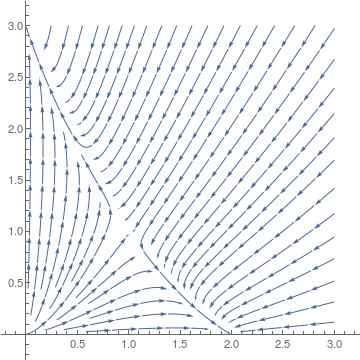
\includegraphics[scale = 0.75]{./_Figures/S13Q6.png}
\end{center}
\noindent From the phase portrait, it is not likely that both species will survive.
\hfill\qed

\subsection*{Solution to Spring 2013, \#7}\label{s137}
We give two solutions. The first is an application of the Cole-Hopf transformation, the second is a direct proof using the maximum principle.

Suppose $u$ solves the given PDE. Let $w := e^{-u}$. Then $w_{t} = -e^{-u}u_{t}$ and $\Delta w = e^{-u}|\nabla u|^{2} - e^{-u}\Delta u$.
Thus in $\Om \times (0, \infty)$,.
$$w_{t} - \Delta w = -e^{-u}u_{t} - e^{-u}|\nabla u|^{2} + e^{-u}\Delta u = -e^{-u}(u_{t} + |\nabla u|^{2} - \Delta u) = 0.$$
It follows that $w$ satisfies
\begin{align}\label{s137eq1}
\begin{cases}
w_{t} - \Delta w = 0 & \text{ in } \Om \times (0, \infty)\\
w(x, t) = e^{-g(x)} & \text{ on } \pr\Om \times (0, \infty)\\
w(x, 0) = e^{-f(x)} & \text{ in } \Om.
\end{cases}
\end{align}
Suppose $w_{1}$ and $w_{2}$ were two distinct solutions to \eqref{s137eq1}. Then let $v := w_{1} - w_{2}$. We have
\begin{align*}
\begin{cases}
v_{t} - \Delta v & \text{ in } \Om \times (0, \infty)\\
v(x, t) = 0 & \text{ on } \pr\Om \times (0, \infty)\\
v(x, 0) = 0 & \text{ in } \Om.
\end{cases}
\end{align*}
Let $E(t) := \frac{1}{2}\int_{\Om}v(x, t)^{2}\, dx$. Then
$$\dot{E}(t) = \int_{\Om}vv_{t}\, dx = \int_{\Om}v\Delta v\, dx = -\int_{\Om}|\nabla v|^{2}\,dx \leq 0.$$
Therefore $v \equiv 0$. Thus the solution to \eqref{s137eq1} is unique. Suppose $u_{1}$, $u_{2}$ were two distinct
solutions to the stated PDE in the problem. Then $w_{1} := e^{-u_{1}}$ and $w_{2} := e^{-u_{2}}$ are two distinct
solutions to \eqref{s137eq1}, a contradiction. Therefore the solution to the stated PDE is unique.

We now present a maximum principle approach.
Suppose both $u$ and $v$ satisfy the PDE where $u \neq v$, and consider $w := u-v$. Fixing $T > 0$, observe that $w$ satisfies the following PDE:
\[
\left\{
\begin{array}{ll}
	w_t - \Delta w + |\del u|^2 - |\del v|^2 = 0 & \text{in} \,\,\, \Omega \times (0,T)\\
	w = 0 & \text{on} \,\,\, \d \Omega \times (0,T) \\
	w(x,0) = 0 & \text{in} \,\,\, \Omega
\end{array}
\right.
\]
Now, define $y = w - \epsilon t$, and observe
\begin{equation}
\label{one}
	y_t - \Delta y + |\del u|^2 - |\del v|^2 = - \epsilon < 0, \quad \quad \text{in} \,\,\, \Omega \times (0,T)
\end{equation}
Because $u$ and $v$ are at least twice differentiable, $w$, and thus $y$, are continuous. It follows that $y$ must attain a maximum at $(x_0,t_0) \in \overline{\Omega} \times [0,T]$. Suppose $(x_0,t_0) \in \Omega \times (0,T)$ (the interior). This would imply
$$y_t(x_0,t_0) = 0, \quad \quad \Delta y(x_0,t_0) \leq 0$$
and
$$\del y(x_0,t_0) = \del w(x_0,t_0) = \del u(x_0,t_0) - \del v(x_0,t_0) = 0 \quad \implies \quad \del u(x_0,t_0) = \del v(x_0,t_0) $$
($\del u$ and $\del v$ must exist everywhere, even at the boundary, since $u$ and $v$ are smooth on the boundary.) Hence,
$$ (y_t - \Delta y + |\del u|^2 - |\del v|^2)(x_0,t_0) = - \Delta y(x_0,t_0) \geq 0 $$
which contradicts \eqref{one}. Hence, the maximum must occur on the boundary. However, $y$ cannot attain its maximum on $\Omega \times \{t=T\}$. To see this, suppose $y$ attains its maximum on $\Omega \times \{t=T\}$ at $(x^*, T)$. This would imply
$$ y_t(x^*,T) \geq 0, \quad \quad \Delta y(x^*,T) \leq 0 $$
$$ \del y(x^*,T) = 0 \quad \implies \quad \del u(x^*,T) = \del v(x^*,T) $$
and hence,
\begin{equation}
\label{s137two}
	(y_t - \Delta y + |\del u|^2 - |\del v|^2)(x^*,T) \geq 0
\end{equation}
Recall that $u$ and $v$ satisfy $u_t - \Delta u + |\del u|^2 = 0$ on $\Omega \times (0,\infty)$, which implies $y = u - v - \epsilon t$ satisfies the
$$ y_t - \Delta y + |\del u|^2 - |\del v|^2 = - \epsilon < 0 $$
on $\Omega \times (0,\infty)$. Thus, \eqref{s137two} would be a contradiction, so $y$ can only attain its maximum on the parabolic boundary of $\Omega \times (0,T)$. Using Evan's notation,
$$ \max_{\bar{\Omega}_T} y = \max_{\Gamma_T} y $$
Now, for all $\epsilon > 0$,
$$ \max_{\Gamma_T} w \geq \max_{\Gamma_T} y = \max_{\bar{\Omega}_T} y \geq \max_{\bar{\Omega}_T} w - \epsilon T $$
so we have
\begin{equation}
\label{s137three}
	\max_{\Gamma_T} w \geq \max_{\bar{\Omega}_T} w
\end{equation}
Since $\Gamma_T \subset \bar{\Omega}_T$, the reverse inequality of \eqref{s137three} is always true, which implies
$$ \max_{\bar{\Omega}_T} w = \max_{\Gamma_T} w $$
Running through the same argument with $w$ replaced by $-w$ will yield
$$ \min_{\bar{\Omega}_T} w = \min_{\Gamma_T} w $$
Hence, because $w = 0$ on the parabolic boundary, $w \equiv 0$ in $\Omega \times (0,T)$. This holds for any $T > 0$, so we've shown that $u=v$ in $\Omega \times (0,\infty)$. Therefore, the solution is unique. \qed

\subsection*{Solution to Spring 2013, \#8}\label{s138}
To show that $u$ is an entropy solution we need to check
\begin{enumerate}
\item $u_{\ell}, u_{r}$ satisfy the PDE in the region of definition
\item Rankine-Hugoniot is satisfied along the shock
\item $F'(u_{\ell}) > \sigma > F'(u_{r})$ on the shock curve
\end{enumerate}
The first two conditions implies that $u$ is an integral solution (via reversing the proof on Page 137-138 of Evans), the last condition is the entropy condition.

In the case of this problem, $u_{r} = -\frac{2}{3}(t + \sqrt{3x + t^{2}})$ and $u_{\ell} = 0$ (since drawing our shock $4x + t^{2} = 0$,
the region where $4x + t^{2} > 0$ is to our left and the region where $4x + t^{2} < 0$ is to our right, note that we draw shock curves in the direction of increasing time).

Observe that $u_{\ell} = 0$ satisfies the PDE. We now check that $(u_{r})_{t} + u_{r}(u_{r})_{x} = 0$. We have
$(u_{r})_{t} = -\frac{2}{3} - \frac{2t}{3}\cdot \frac{1}{\sqrt{3x + t^{2}}}$ and $(u_{r})_{x} = -\frac{1}{\sqrt{3x + t^{2}}}$.
Therefore
$$(u_{r})_{t} + u_{r}(u_{r})_{x} = (-\frac{2}{3} - \frac{2t}{3}\cdot \frac{1}{\sqrt{3x + t^{2}}}) + (-\frac{2}{3}t - \frac{2}{3}\sqrt{3x + t^{2}})(-\frac{1}{\sqrt{3x + t^{2}}}) = 0.$$

Next we check that the Rankine-Hugoniot conditions are satisfied. Let $F(s) := s^{2}/2$. Then
\begin{align*}
\frac{F(u_{\ell}) - F(u_{r})}{u_{\ell} - u_{r}} = \frac{F(u_{r})}{u_{r}} = \frac{1}{2}u_{r}.
\end{align*}
On the shock curve, that is, on the curve $x = -t^{2}/4 =: s(t)$,
\begin{align*}
\frac{1}{2}u_{r} = \frac{1}{2}(-\frac{2}{3}(t + \sqrt{3x + t^{2}})) = -\frac{1}{3}(t + \sqrt{-\frac{3}{4}t^{2} + t^{2}}) = -\frac{1}{3}(t + \frac{t}{2}) = -\frac{1}{2}t = \dot{s}(t).
\end{align*}
Therefore the solution satisfies the Rankine-Hugoniot condition.

Lastly we check that the entropy condition is satisfied. We have $\sigma = \dot{s}(t) =-\frac{1}{2}t$ and $F'(u_{\ell}) = u_{\ell}$ and $F'(u_{r}) = u_{r}$.
When $x = -t^{2}/4 = s(t)$,
$$0 > -\frac{1}{2}t > -\frac{2}{3}(t + \sqrt{3x + t^{2}})$$
since in this case
$$-\frac{2}{3}(t + \sqrt{3x + t^{2}}) = -\frac{2}{3}(t + \frac{t}{2}) = -t.$$
Therefore the entropy conidtion is satisfied on the shock curve and hence $u$ is an entropy solution of the equation
$u_{t} + uu_{x} = 0$.
\hfill\qed


\section{Fall 2012}\label{f12}
\subsection*{Solution to Fall 2012, \#1}
\label{F12Q1}

Suppose $u$ and $v$ are solutions to the PDE, and define $w:=u-v$. Observe that $w$ now satisfies
$$ \left\{
\begin{array}{ll}
	\Delta w = 0 & \text{for} \,\, |x| < 1, \,\, |y| < 1 \\
	w = 0 & \text{for} \,\, |x| = 1, \,\, |y| \leq 1 \\
	w_x = w_y & \text{for} \,\, |y| = 1, \,\, |x| < 1
\end{array}
\right.
$$
There are (at least) two ways of solving this problem --- both will be explained.

The first method uses the maximum principle for harmonic functions. Define
\begin{gather*}
	D := \{ (x,y) \, | \, |x| < 1, \, |y| < 1 \} \\
	\Gamma_1 := \{ (x,y) \, | \, |x|=1, \, |y| \leq 1 \} \\
	\Gamma_2 := \{ (x,y) \, | \, |y|=1, \, |x|<1 \}
\end{gather*}
Note that $\Gamma_1$ contains the corners of the square domain. Because $w$ is harmonic in $D$, the maximum of $w$ must occur on $\d D = \Gamma_1 \cup \Gamma_2$. If the maximum of $w$ occurs on $\Gamma_1$, then $w \leq 0$ in $D$. Now, suppose the maximum of $w$ occurs on $\Gamma_2$ at $(x_0,y_0)$, and furthermore, suppose this is a strict maximum. If not, then, by the strong maximum principle, $w$ is constant on $D$. This would mean $w \equiv 0$ since $w = 0$ on $\Gamma_1$, implying that the solution is unique. So, if $w$ achieves a strict maximum on $\Gamma_2$, then, by Hopf's Lemma,
$$\frac{\d w}{\d y}(x_0,y_0) = \frac{\d w}{\d x}(x_0,y_0) > 0 $$
Note that we can apply Hopf's Lemma here because $\Gamma_2$ satisfies the interior ball property (this is why we chose to let $\Gamma_1$ contain the corners of the domain). However, since $w_x(x_0,y_0)$ is strictly positive, this would imply that $w$ does not achieve its maximum at $(x_0,y_0)$. Thus, by contradiction, if a maximum were to occur on $\Gamma_2$, it can't be a strict maximum, implying that $w \equiv 0$. Hence, we've shown that either $w \leq 0$ or $w \equiv 0$ on $D$.

Swapping the roles of $u$ and $v$ will yield $w \geq 0$ or $w \equiv 0$ on $D$. Therefore, $w \equiv 0$, implying that the solution is unique.

\vspace{0.4cm}

The second method uses integration by parts. Multiplying the PDE by $w$ and integrating both sides yields
\begin{align*}
0 &= \int_D \Delta w w \, dx \\
&= - \int_D |\nabla w|^2 \, dx + \int_{\d D} \frac{\d w}{\d \nu} w \, dSx	
\end{align*}
where $\nu$ is the unit outer normal. Since $w = 0$ on $\Gamma_1$, we only need to worry about $\Gamma_2$. Observe,
\begin{align*}
\int_{\d D} \frac{\d w}{\d \nu} w \, dSx &= \int_{\Gamma_2} \frac{\d w}{\d \nu} w \, dSx \\
&= \int_{1}^{-1} w_y(x,1) w(x,1) \, dx + \int_{-1}^1 -w_y(x,-1) w(x,-1) \, dx
\end{align*}
where the first integral is for the top portion of $\Gamma_2$ and the second integral is for the bottom portion of $\Gamma_2$. Now, we compute
$$ \int_1^{-1} w_y(x,1) w(x,1) \, dx = \int_1^{-1} w_x(x,1) w(x,1) \, dx = \frac{1}{2} \int_1^{-1} (w(x,1)^2))_x \, dx = 0$$
where the last equality is because of the boundary conditions on $w$. Similarly,
$$ \int_{-1}^1 -w_y(x,-1)w(x,-1) \, dx = 0 $$
Hence, we have
$$ 0 = -\int_D |\nabla w|^2 \, dx $$
implying that $u$ is constant in $D$. However, because $w = 0$ on $\Gamma_1$, we have that $w \equiv 0$ in $D$. Therefore, the solution to the PDE is unique. \qed




\subsection*{Solution to Fall 2012, \#2}
\label{F12Q4}

\subsubsection*{Solution to $2a$}

We compute
$$ \frac{d}{dt} \int_{\R^2} \rho(x,t)\, dx = \int_{\R^2} \rho_t(x,t) \, dx = \int_{\R^2} \Delta (\rho^2) + \nabla \cdot (2x \rho) \, dx $$
Observe that, because $\rho$ is compactly supported for all time $t>0$, using integration by parts yields
$$ \int_{\R^2} \Delta (\rho^2) \, dx = 0 $$
Furthermore,
$$ \int_{\R^2} \nabla \cdot (2x \rho) \, dx  = \int_{\R^2} 2n\rho + 2x \cdot \nabla \rho \, dx $$
Then, by integration by parts, the above boils down to
$$ \int_{\R^2} \nabla \cdot (2x \rho) \, dx = \int_{\R^2} 2n \rho - 2n \rho \, dx = 0$$
Again, because $\rho$ is compactly supported for all $t>0$, the boundary terms vanish. Thus,
$$ \frac{d}{dt} \int_{\R^2} \rho(x,t) \, dx = 0 $$
implying that
$$ \int_{\R^2} \rho(x,t) \, dx = \int_{\R^2} \rho(x,0) \, dx = 1 $$
\hfill \qed

\subsubsection*{Solution to $2b$}

Again, we will take a time derivative of the integral.
$$ \frac{d}{dt} \int_{\R^2} \rho^2 + \rho |x|^2 + C \rho \, dx = \int_{\R^2} 2 \rho \rho_t + \rho_t |x|^2 \, dx $$
Note that, because of part (a), $\int_{\R^2} C \rho \, dx = C$, so that term vanishes after taking a time derivative. Continuing with our computations, we have
\begin{align*}
\int_{\R^2} \rho_t(2\rho + |x|^2) \, dx &= \int_{\R^2} \left( \Delta  (\rho^2) + \nabla \cdot (2x \rho) \right) \left( 2\rho + |x|^2 \right) \, dx \\
&= -\int_{\R^2} (\nabla (\rho^2) + 2x \rho) \cdot \nabla (2\rho + |x|^2) \, dx \\
&= -\int_{\R^2} \rho (2 \nabla \rho + 2x) \cdot (2\nabla \rho + 2x) \, dx \\
&= -\int_{\R^2} \rho |2 \nabla \rho + 2x|^2 \, dx \leq 0
\end{align*}
because $\rho$ is assumed to be nonnegative for all time $t>0$. Note, the second inequality is from applying integration by parts. Again, the boundary terms vanish because $\rho$ is compactly supported for all time $t>0$. Hence, the energy is non-increasing for any choice of $C$. (I don't think we have enough to show that the energy is \emph{decreasing}.)

\subsubsection*{Solution to $2c$}

Since the energy is both positive and non-increasing, we know that the energy is either constant or it's decreasing to 0. In both cases, we can make the conclusion that as $t \to \infty$,
$$ \frac{d}{dt} \int_{\R^2} \rho^2 + \rho|x|^2 + C \rho \, dx = -\int_{\R^2} \rho |2 \nabla \rho + 2x|^2 \, dx \to 0$$
This implies that either $\rho \to 0$ or $2 \nabla \rho + 2x \to 0$ as $t \to \infty$. Because of our work in part (a), the first option can't hold, so we have\
\begin{align*}
2 \nabla \rho + 2x \to 0 \quad &\implies \quad \nabla \rho \to -x \\
&\implies \quad \rho \to C_0 -\frac{|x|^2}{2}\
\end{align*}
Because $\rho$ is nonnegative for all time $t>0$, we must have $ \rho \to \left( C_0 - \frac{|x|^2}{2} \right)_+$ as $t \to \infty$. To find $C_0$, we use part (a).
\begin{align*}
\int_{\R^2} \rho(x,t) \, dx = 1 \quad &\implies \quad \int_{\R^2} \left( C_0 - \frac{|x|^2}{2} \right)_+ \, dx = 1 \\
&\implies \quad \int_{B(0,\sqrt{2C_0})} C_0 - \frac{|x|^2}{2} \, dx = 1 \\
&\implies \quad \int_0^{2\pi} \int_0^{\sqrt{2C_0}} \left( C_0 - \frac{r^2}{2} \right) r \, dr d\theta = 1\\
&\implies \quad 2 \pi \left( C_0^2 - \frac{C_0^2}{2} \right) = 1 \\
&\implies \quad C_0 = \frac{1}{\sqrt{\pi}}
\end{align*}
\hfill \qed











\subsection*{Solution to Fall 2012, \#3}
\label{F12Q3}

Letting $v := u'$, we can rewrite the second-order ODE into a first-order system:
\begin{align*}
u' &= v \\
v' &= -f(u) + \lambda v
\end{align*}
Define $F : \R^2 \to \R^2$ as $F(u,v) = (v, -f(u) + \lambda v)$, and observe that
$$ \nabla \cdot F(u,v) = \lambda > 0 $$
Thus, by the Bendixson-Dulac theorem, the ODE has no periodic solutions other than any stationary equilibrium solutions ($u \equiv c \in \R$). \hfill \qed












\subsection*{Solution to Fall 2012, \#4}

Let $u(x, t) = f(x + t)$ with $f$ having a jump discontinuity at $x = x_{0}$ and fix an $v \in C_{0}^{\infty}(\R \times [0, \infty))$. Since we will want to show that
$f(x + t)$ is a weak solution to the wave equation, we will assume $g$ is the weak derivative of $f$.
We have
\begin{align}\label{F124eq1}
\int_{0}^{\infty}&\int_{-\infty}^{\infty}f(x + t)v_{tt}\, dx\, dt = \int_{-\infty}^{\infty}\int_{0}^{\infty}f(x + t)v_{tt}\, dt\, dx\nonumber\\
&= \int_{-\infty}^{\infty}1_{x_{0} - x \geq 0}\int_{0}^{\infty}f(x + t)v_{tt}\, dt\, dx + \int_{-\infty}^{\infty}1_{x_{0} - x < 0}\int_{0}^{\infty}f(x + t)v_{tt}\, dt\, dx\nonumber\\
&= \int_{-\infty}^{x_{0}}\bigg(\int_{0}^{x_{0} - x}f(x + t)v_{tt}\, dt + \int_{x_{0} - x}^{\infty}f(x + t)v_{tt}\, dt\bigg)\, dx + \int_{x_{0}}^{\infty}\int_{0}^{\infty}f(x + t)v_{tt}\, dt\, dx.
\end{align}
Since $v$ is of compact support and
$$\int_{a}^{b}f(x + t)v_{tt}\, dt = f(x + b)v_{t}(x, b) - f(x + a)v_{t}(x, a) - \int_{a}^{b}f'(x + t)v_{t}\, dt,$$
we have that \eqref{F124eq1} is equal to
\begin{equation}
\begin{aligned}\label{F124eq2}
\int_{-\infty}^{x_{0}}&\bigg(f_{-}(x_{0})v_{t}(x, x_{0} - x) - f(x)v_{t}(x, 0) - \int_{0}^{x_{0} - x}f'(x + t)v_{t}\, dt - f_{t}(x_{0})v_{t}(x, x_{0} - x)\\
&\quad\quad\quad - \int_{x_{0} - x}^{\infty}f'(x + t)v_{t}\, dt\bigg)\, dx + \int_{x_{0}}^{\infty}-f(x)v_{t}(x, 0)\, dx - \int_{0}^{\infty}f'(x + t)v_{t}\, dt\, dx\\
&= (f_{-}(x_{0}) - f_{+}(x_{0}))\int_{-\infty}^{x_{0}}v_{t}(x, x_{0} - x)\, dx - \int_{-\infty}^{\infty}f(x)v_{t}(x, 0)\, dx - \int_{0}^{\infty}\int_{-\infty}^{\infty}f'(x + t)v_{t}\, dx\, dt.
\end{aligned}
\end{equation}
Since $v$ is of compact support and
$$\int_{a}^{b}f'(x + t)v_{t}\, dx = f(b + t)v_{t}(b, t) - f(a + t)v_{t}(a, t) - \int_{a}^{b}f(x + t)v_{tx}\, dx$$
we have
\begin{equation}
\begin{aligned}\label{F124eq3}
\int_{0}^{\infty}\int_{-\infty}^{\infty}f'(x + t)v_{t}\, dx\, dt &= \int_{0}^{\infty}\bigg(\int_{-\infty}^{x_{0} - t}f'(x + t)v_{t}\, dx + \int_{x_{0} - t}^{\infty}f'(x + t)v_{t}\, dx\bigg)\, dt\\
&= (f_{-}(x_{0}) - f_{+}(x_{0}))\int_{0}^{\infty}v_{t}(x_{0} - t, t)\, dt - \int_{0}^{\infty}\int_{-\infty}^{\infty}f(x + t)v_{tx}\, dx\, dt.
\end{aligned}
\end{equation}
A change of variables shows that
$\int_{0}^{\infty}v_{t}(x_{0} - t, t)\, dt = \int_{-\infty}^{x_{0}}v_{t}(x, x_{0} - x)\, dx$
and hence combining this with \eqref{F124eq1}-\eqref{F124eq3} yields
\begin{align}\label{F124eq5}
\int_{0}^{\infty}&\int_{-\infty}^{\infty}f(x + t)v_{tt}\, dx\, dt = -\int_{-\infty}^{\infty}f(x)v_{t}(x, 0)\, dx + \int_{0}^{\infty}\int_{-\infty}^{\infty}f(x + t)v_{tx}\, dx\, dt.
\end{align}
We now similarly consider the $v_{xx}$ term. For $t \in [0, \infty)$, note that $x_{0} - t \in (-\infty, \infty)$.
Since
$$\int_{a}^{b}f(x + t)v_{xx}\, dx = f(b + t)v_{x}(b, t) - f(a + t)v_{x}(a, t) - \int_{a}^{b}f'(x + t)v_{x}\, dx,$$
we have
\begin{align*}
\int_{0}^{\infty}\int_{-\infty}^{\infty}f(x + t)v_{xx}\, dx\, dt &= \int_{0}^{\infty}\bigg(\int_{-\infty}^{x_{0} - t}f(x + t)v_{xx}\, dx + \int_{x_{0} - t}^{\infty}f(x + t)v_{xx}\, dx\bigg)\, dt\\
&= (f_{-}(x_{0}) - f_{+}(x_{0}))\int_{0}^{\infty}v_{x}(x_{0} - t, t)\, dt - \int_{0}^{\infty}\int_{-\infty}^{\infty}f'(x + t)v_{x}\, dx\, dt.
\end{align*}
Similarly to the calculations done at the beginning of this solution,
\begin{align*}
\int_{0}^{\infty}\int_{-\infty}^{\infty}&f'(x + t)v_{x}\, dx\, dt = \int_{-\infty}^{\infty}\int_{0}^{\infty}f'(x + t)v_{x}\, dt\, dx\\
&= \int_{-\infty}^{\infty}\bigg(1_{x_{0} - x \geq 0}\int_{0}^{\infty}f'(x + t)v_{x}\, dt + 1_{x_{0} - x < 0}\int_{0}^{\infty}f'(x + t)v_{x}\, dt\bigg)\, dx\\
&= \int_{-\infty}^{x_{0}}\bigg(\int_{0}^{x_{0} - x}f'(x + t)v_{x}\, dt + \int_{x_{0} - x}^{\infty}f'(x + t)v_{x}\, dt\bigg)\, dx + \int_{x_{0}}^{\infty}\int_{0}^{\infty}f'(x + t)v_{x}\, dt\, dx.
\end{align*}
Since
$$\int_{a}^{b}f'(x + t)v_{x}\, dt = f(x + b)v_{x}(x, b) - f(x + a)v_{x}(x, a) - \int_{a}^{b}f(x + t)v_{xt}\, dt,$$
it follows that
\begin{align*}
\int_{0}^{\infty}&\int_{-\infty}^{\infty}f'(x + t)v_{x}\, dx\, dt\\
& = (f_{-}(x_{0}) - f_{+}(x_{0}))\int_{-\infty}^{x_{0}}v_{x}(x, x_{0} - x)\, dx - \int_{-\infty}^{\infty}f(x)v_{x}(x,0)\, dx - \int_{-\infty}^{\infty}\int_{0}^{\infty}f(x + t)v_{xt}\, dt\, dx.
\end{align*}
Again by a change of variables $\int_{0}^{\infty}v_{x}(x_{0} - t, t)\, dt =\int_{-\infty}^{x_{0}}v_{x}(x, x_{0} - x)\, dx$ and hence
\begin{align}\label{F124eq6}
\int_{0}^{\infty}\int_{-\infty}^{\infty}f(x + t)v_{xx}\, dx\, dt = \int_{-\infty}^{\infty}f(x)v_{x}(x, 0)\, dx + \int_{-\infty}^{\infty}\int_{0}^{\infty}f(x + t)v_{xt}\, dt\, dx.
\end{align}
Subtracting \eqref{F124eq6} from \eqref{F124eq5} yields
\begin{align*}
\int_{0}^{\infty}\int_{-\infty}^{\infty}f(x + t)(v_{tt} - v_{xx})\, dx\, dt& = -\int_{-\infty}^{\infty}f(x)v_{t}(x, 0)\, dx - \int_{-\infty}^{\infty}f(x)v_{x}(x, 0)\, dx\\
& = -\int_{-\infty}^{\infty}f(x)v_{t}(x, 0)\, dx + \int_{-\infty}^{\infty}g(x)v(x, 0)\, dx
\end{align*}
where in the last equality we have used that the weak derivative of $f$ is $g$.
This shows that $u(x, t) = f(x + t)$ is a weak solution of the wave equation.
\hfill\qed

\subsection*{Solution to Fall 2012, \#5}
\label{F12Q5}

\subsubsection*{Solution to $5a$}

We convert to polar coordinates. Let $x = r\cos\theta$ and $y = r\sin \theta$. Then,
\begin{align*}
r^2 =x^2 + y^2 \quad &\implies \quad r\dot{r} = x\dot{x} + y \dot{y} \\
&\implies \quad \dot{r} = \dot{x} \cos \theta + \dot{y} \sin \theta \\
&\implies \quad \dot{r} = (-r^{2a+1} \sin \theta) \cos \theta + (r^{2a+1} \cos \theta) \sin \theta \\
&\implies \quad \dot{r} = 0
\end{align*}
and
\begin{align*}
\tan \theta = \frac{y}{x} \quad &\implies \quad (\sec^2 \theta) \dot{\theta} = \frac{x \dot{y} - y \dot{x}}{x^2} \\
&\implies \quad \dot{\theta} = \frac{(r \cos \theta)(r^{2a+1} \cos \theta)+(r \sin \theta)(r^{2a+1} \sin \theta)}{r^2} \\
&\implies \quad \dot{\theta} = r^{2a}
\end{align*}
Hence, we have $r = C$ and $\theta = C^{2a}t + \tilde{C}$ for constants $C$ and $\tilde{C}$. In this case, the trajectories are circles and the system is globally well-posed forward and backward in time as long as don't have both $r(0) = 0$ and $a < 0$. \hfill \qed

\subsubsection*{Solution to $5b$}

This time, going thorugh similar calculations as in part (a), we have
$$\dot{r} = -r^{2a+1} \quad \text{and} \quad \dot{\theta} = 0 $$
Solving the ODEs yield
$$ r^{-2a} = 2at - 2aC \quad \text{and} \quad \theta = \tilde{C} $$
for constants $C$ and $\tilde{C}$.

If $a < 0$, let $b = -a$ (for ease of notation). Then, $r^{2b} = -2bt + 2bC$, implying that
$$ r = \left( 2bC - 2bt \right)^{1/2b}, \quad \text{where} \quad C = \frac{r(0)^{2b}}{2b} = \frac{r(0)^{2|a|}}{2|a|} $$
In this case, the system is globally well-posed backward in time. The system is only locally well-posed forward in time since we can only solve until time
$$ t = C = \frac{r(0)^{2|a|}}{2|a|} $$
before the radius becomes undefined. For this case, as $t \to -\infty$, the trajectory starts from $r=r(0)$ and traces a ray (that starts at the origin and forms an angle of $\theta = \tilde{C}$ with the $x$-axis) out to infinity. As $t \to C^-$, the trajectory starts from $r=r(0)$ and traces the same ray toward the origin. Note that we will actually reach the origin before well-posedness breaks.

If $a > 0$, we have
$$ r = \left( \frac{1}{2at - 2aC} \right)^{1/2a}, \quad \text{where} \quad C = \frac{r(0)^{-2a}}{-2a} $$
In this case, the system is globally well-posed forward in time. The system is only locally well-posed backward in time since we can only solve until time
$$ t = C = \frac{r(0)^{-2a}}{-2a} $$
before the radius blows up. For this case, as $t \to \infty$, the trajectory starts from $r=r(0)$ and traces a ray (that starts at the origin and forms an angle of $\theta = \tilde{C}$ with the $x$-axis) toward the origin, only getting arbitrarily close to the origin. As $t \to C^+$, the trajectory starts from $r=r(0)$ and traces the same ray toward infinity. Because we can only get arbitrarily close to the origin, we also require $r(0) \neq 0$ for this case. \hfill \qed

\subsection*{Solution to Fall 2012, \#6}
\label{F12Q6}

\subsubsection*{Solution to $6a$}

We used generalized method of characteristics to solve this problem, which is analogous to method of characteristics in one dimension. We have
$$
\begin{array}{lll}
\asep
\dot{t}(s) = 1, \quad t(0) = 0 & \implies & t(s) = s \\ \asep
\dot{\vx}(s) = \vz(s), \quad \vx(0) = \vx_0 & \implies & \vx(s) = \vx(t) = \vu_0(\vx_0)t + \vx_0 \\ \asep
\dot{\vz}(s) = 0, \quad \vz(0) = \vu_0(\vx_0) & \implies & \vz(s) = \vz(t) = \vu_0(\vx_0)
\end{array}
$$
Therefore,
$$ \vu(\vx,t) = \vu_0 (\vr) \quad \text{where} \quad \vx = \vu_0(\vr) t + \vr $$
\hfill \qed

\subsubsection*{Solution to $6b$}

We compute
$$ \vu(\vx,t) = \vu_0(\vr) \quad \implies \quad \frac{\d \vu}{\d \vx} = \frac{\d \vu_0}{\d \vx}(\vr) \frac{\d \vr}{\d \vx} $$
and
\begin{align*}
\vx = \vu_0(\vr) t + \vr \quad &\implies \quad \operatorname{Id} = \frac{\d \vu_0}{\d \vx}(\vr) \frac{\d \vr}{\d \vx} t + \frac{\d \vr}{\d \vx} \\
&\implies \quad \frac{\d \vr}{\d \vx} = \left[ \frac{\d \vu_0}{\d \vx}(r) t + \operatorname{Id} \right]^{-1}
\end{align*}
Thus,
$$ \frac{\d \vu}{\d \vx} = \frac{\d \vu_0}{\d \vx} (r) \left[ \frac{\d \vu_0}{\d \vx}(r) t + \operatorname{Id} \right]^{-1} $$
Let $\lambda$ be an eigenvalue of $\frac{\d \vu_0}{\d \vx}$. Then, eigenvalues of $\frac{\d \vu}{\d \vx}$ are of the form $\frac{\lambda}{1 + t\lambda}$. To see this, let $v$ be the corresponding eigenvector to $\lambda$ for $\frac{\d \vu_0}{\d \vx}$. Then,
\begin{align*}
\left[ \frac{\d \vu_0}{\d \vx}(r) t + \operatorname{Id} \right] v = t\lambda v + v = (1 + \lambda t) v \quad &\implies \quad \left(\left[ \frac{\d \vu_0}{\d \vx}(r) t + \operatorname{Id} \right]^{-1} \right)v = (1+\lambda t)^{-1} v \\
&\implies \quad \left(\frac{\d \vu_0}{\d \vx} (r) \left[ \frac{\d \vu_0}{\d \vx}(r) t + \operatorname{Id} \right]^{-1} \right)v = \lambda (1+ \lambda t)^{-1} v
\end{align*}
Since $\left| \frac{\d \vu}{\d \vx} \right| > \rho\left( \frac{\d \vu}{\d \vx} \right)$, where
$$ \rho\left( \frac{\d \vu}{\d \vx} \right) = \max \left\{ \frac{|\lambda|}{|1+t\lambda|} \, : \, \lambda \,\, \text{eigenvalue of} \,\, \frac{\d \vu_0}{\d \vx} \right\}$$
we have finite time blow up of $\left| \frac{\d \vu}{\d \vx} \right|$ if $ \frac{\d \vu_0}{\d \vx} $ has at least one negative eigenvalue. \hfill \qed














\subsection*{Solution to Fall 2012, \#7}
\label{F12Q7}

Suppose $w_n \in X_n$ is the function that minimizes the Rayleigh quotient and $m_n$ is the value of the Rayleigh quotient of evaluateed at $w_n$. That is,
\[
m_n = \frac{||\del w_n||^2}{||w_n||^2}
\]
We first show that $m_n$ is the eigenvalue associated to the function $w_n$. Let $v \in X_n$ be an arbitrary test function, and consider
\[
f(\ep) := \frac{|| \del (w_n+\ep v)||^2}{||w_n+\ep v||^2}
\]
Observe that $f$ has a minimum at $\ep = 0$, which implies that $f'(0) = 0$. Thus, we have
\begin{align*}
\lim_{\ep \to 0} \frac{f(\ep) - f(0)}{\ep} &= \lim_{\ep \to 0} \frac{1}{\ep} \left[ \frac{ || \del w_n||^2 + 2\ep \langle \del w_n, \del v \rangle + \ep^2 ||\del v||^2}{||w_n||^2 + 2\ep \langle w_n, v \rangle + \ep^2 ||v||^2} - \frac{|| \del w_n||^2}{||w_n||^2} \right] \\
&= \frac{2 \langle \del w_n, \del v \rangle ||w_n||^2 - 2 \langle w_n, v \rangle ||\del w_n||^2}{||w_n||^4} = 0
\end{align*}
It then follows that
\begin{align*}
\langle \del w_n, \del v \rangle ||w_n||^2  = \langle w_n,v \rangle ||\del w_n||^2 \quad &\implies \quad  \langle \del w_n, \del v \rangle = m_n \langle w_n, v\rangle \\
&\implies \quad \int_{\Omega} \del w_n \cdot \del v \, dx = m_n \int_{\Omega} w_nv \, dx \\
&\implies \quad -\int_{\Omega} \lap w_n v \, dx = m_n \int_{\Omega} w_nv \, dx
\end{align*}
where the final line above is a result of integration by parts. The boundary terms vanish because of the homogeneous Neumann boundary condition. Hence, for all $v \in X_n$, we have
\[
\int_{\Omega} (\lap w_n + m_n w_n) v \, dx = 0
\]
We now aim to show that the same is true for all test functions $v \in H^1(\Omega)$, Let $v \in H^1(\Omega)$ be an arbitrary test function. Let $g$ be defined so that
\[
g(x) = v(x) - \sum_{k=1}^{n-1} c_k v_k(x), \quad \text{where} \quad c_k = \frac{ \langle v, v_k \rangle}{\langle v_k, v_k \rangle}
\]
where $v_i$ for $i=1, \dots, n-1$ are the first $n-1$ eigenfunctions. Then,
\begin{align}
\notag \int_{\Omega} (\lap w_n + m_n w_n)v \, dx  &= \int_{\Omega} (\lap w_n + m_n w_n) \left( g + \sum_{k=1}^{n-1} c_k v_k \right) \, dx \\
\label{f127eq} &= \int_{\Omega} (\lap w_n + m_n w_n)g\, dx + \int_{\Omega} (\lap w_n + m_n w_n) \left( \sum_{k=1}^{n-1} c_k v_k \right) \, dx
\end{align}
We aim to show that both integrals of \eqref{f127eq} are 0. First, we claim that $\langle g, v_i \rangle = 0$ for $i = 1, \dots, n-1$.
\begin{align*}
\langle g, v_i \rangle &= \langle v - \sum_{k=1}^{n-1} c_k v_k, v_i \rangle \\
&= \langle v, v_i \rangle - \sum_{k=1}^{n-1} c_k \langle v_k, v_i \rangle \\
&= \langle v, v_i \rangle - c_i \langle v_i, v_i \rangle \\
&= 0
\end{align*}
Hence, $g \in X_n$, so by our work above
$$
\int_{\Omega} (\Delta w_n + m_n w_n )g \, dx = 0
$$
Next, observe that, for $k = 1, \dots, n-1$,
\begin{align*}
\int_{\Omega} (\lap w_n + m_n w_n) v_k \, dx &= \int_{\Omega} \lap v_k w_n + m_n w_n v_k \, dx \\
&= (-\lambda_k + m_n) \int_{\Omega} w_n v_k \, dx
\end{align*}
But, since $w_n \in X_n$, $\langle w_n, v_k \rangle = 0$. This implies that
$$
\int_{\Omega} (\lap w_n + m_n w_n) \left( \sum_{k=1}^{n-1} c_k v_k \right) \, dx = 0
$$
Thus, applying these two results to \eqref{f127eq} yields
\[
\int_{\Omega} (\lap w_n + m_n w_n)v \, dx = 0
\]
for all test functions $v \in Y$. Thus, we get $m_n$ is the eigenvalue associated with the eigenfunction $w_n$.

Since $X_n \subset X_{n-1} \subset \cdots \subset X$, we have that $m_n \geq \lambda_{n-1} \geq \cdots \geq \lambda_1$. We can also show $\lambda_{n+1}, \lambda_{n+2}, \dots$ are all bigger than $m_n$. For $k \geq n+1$, let $v_k$ be an eigenfunction with eigenvalue $\lambda_k$. Observe that $\langle v_k, v_i \rangle = 0$ for $ i = 1, \dots, n-1$, which implies $v_k \in X_n$. Then,
\[
m_n = \frac{|| \del w_n||^2}{||w_n|^2} \leq \frac{|| \del v_k||^2}{||v_k||^2} = \frac{\int_{\Omega} -\lap v_k v_k \, dx}{\int_{\Omega} v_k^2 \, dx} = \frac{\lambda_k \int_{\Omega} v_k^2 \, dx}{\int_{\Omega} v_k^2 \, dx} = \lambda_k
\]
Therefore, the result holds. \hfill \qed


\subsection*{Solution to Fall 2012, \#8}
\label{F12Q8}

We use method of characteristics to solve this problem. Also, because the initial data is periodic, we'll initially only work on the interval $[0,4]$. We have
$$
\begin{array}{lll}
\asep
\dot{t}(s) = 1, \quad t(0) = 0 & \implies & t(s) = s \\ \asep
\dot{x}(s) = z(s), \quad x(0) = x_0 & \implies & x(s) = x(t) = u_0(x_0)t + x_0 \\ \asep
\dot{z}(s) = 0, \quad z(0) = u_0(x_0) & \implies & z(s) = z(t) = u_0(x_0)
\end{array}
$$
Therefore,
$$ u(x,t) = u_0 (x_0) \quad \text{where} \quad x = u_0(x_0) t + x_0 $$
where $x_0 \in [0,4]$. Then,
\[
u_0(x_0) = \left\{
\begin{array}{ll}
 2 & \text{if} \,\,\, 0 < x_0 < 2 \quad \implies \quad x = 2t+x_0 \\
 0 & \text{if} \,\,\, 2 < x_0 < 4 \quad \implies \quad x = x_0
\end{array}
\right.
\]
Hence, so far, we have
\[
u(x,t) = \left\{
\begin{array}{ll}
 2 & \text{if} \,\,\, 0 < x-2t < 2 \\
 0 & \text{if} \,\,\, 2 < x < 4
\end{array}
\right.
\]
Extending this by periodicity of the initial data, we have, for $k \in \Z$,
\[
u(x,t) = \left\{
\begin{array}{ll}
 2 & \text{if} \,\,\, 4k < x-2t < 4k+2 \\
 0 & \text{if} \,\,\, 4k+2 < x < 4k+4
\end{array}
\right.
\]
which yields the following picture.

\begin{center}
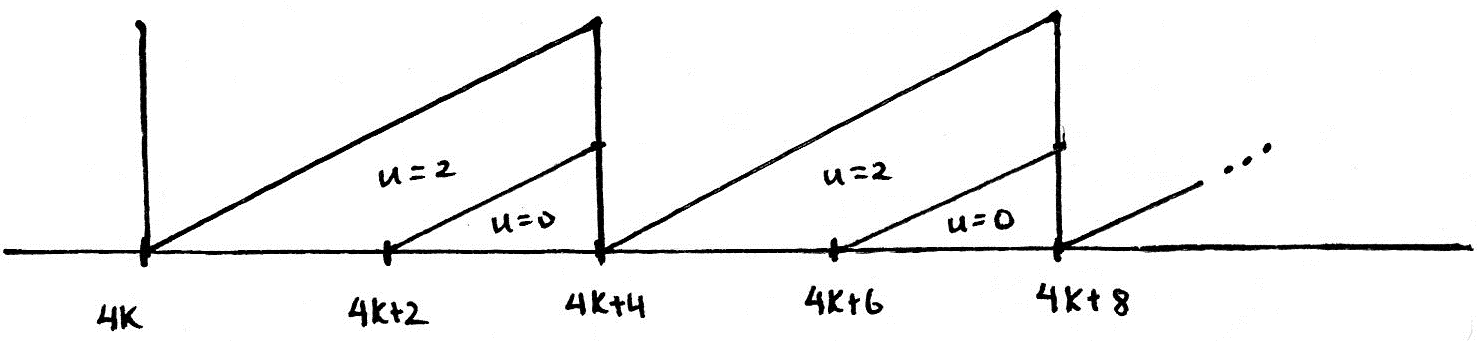
\includegraphics[scale=0.4]{./_Figures/f128img1.png}
\end{center}

Notice that characteristics crash immediately at $x(0) = 4k+2$ for $k \in \Z$. By the Rankine-Hugoniot condition, the shock curves are given by
$$ \dot{x}(t) = \frac{f(u_l) - f(u_r)}{u_l-u_r} = \frac{\frac{1}{2}(2)^2}{2} = 1, \quad x(0) = 4k+2 \quad \implies \quad x(t) = t+4k+2$$
\newpage
Hence, so far, we have the following picture:

\begin{center}
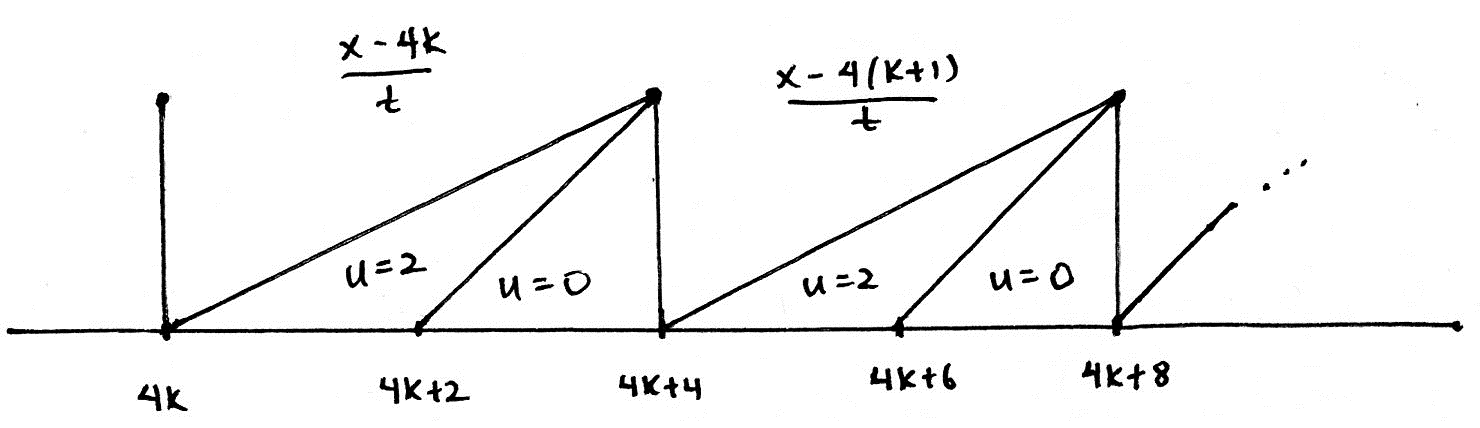
\includegraphics[scale=0.4]{./_Figures/f128img2.png}
\end{center}

Now, we fill in the regions $ \left\{ 4k < x < 4k+2t \right\}$ with rarefaction waves, which we define as $u = \frac{x-4k}{t}$. However, the characteristics $x = 4k+2t$ crash into the characteristics $x=4(k+1)$, which forms new shock curves. By Rankine-Hugoniot, these shocks are defined by
$$ \dot{x}(t) = \dfrac{\frac{1}{2} \left( \frac{x-4k}{t} \right)^2 - \frac{1}{2} \left( \frac{x-4(k+1)}{t} \right)^2}{\frac{x-4k}{t} - \frac{x-4(k+1)}{t}}, \quad x(2) = 4(k+1) $$
for $k \in \Z$. Solving this yields $x = t + 4k + 2$. Hence, our solution satisfies the following picture:

\begin{center}
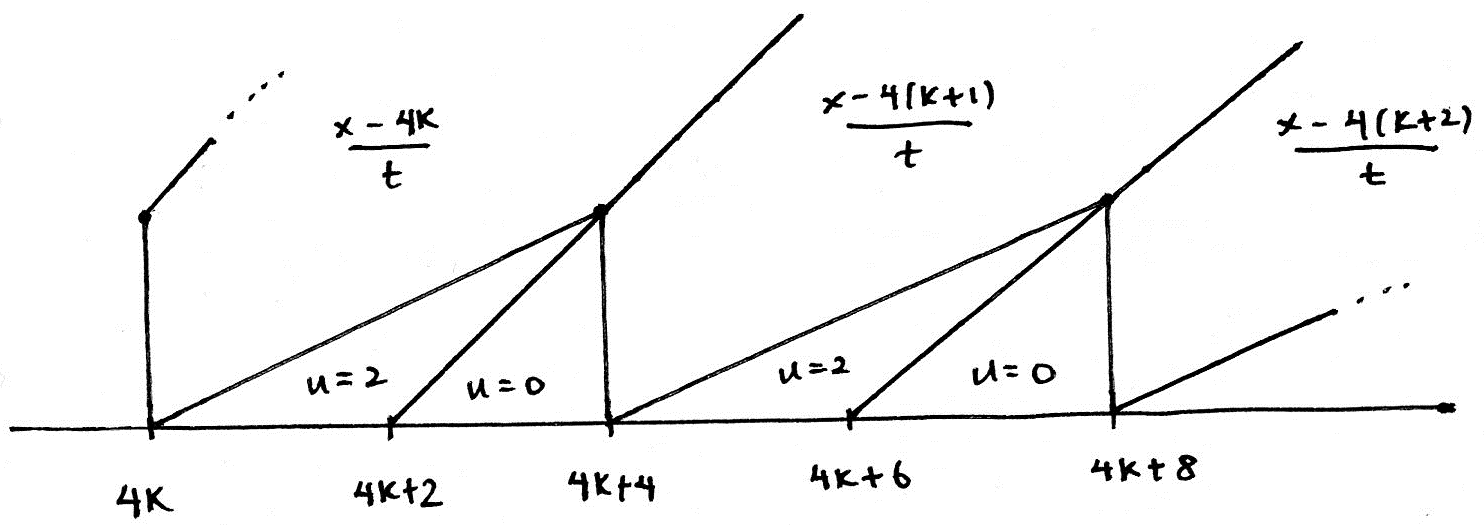
\includegraphics[scale=0.4]{./_Figures/f128img3.png}
\end{center}

Therefore, the slope of the solution, $\frac{\d u}{\d x}$, is $\frac{1}{t}$ almost everywhere for $t>2$. \hfill \qed


\section{Spring 2012}\label{s12}
\subsection*{Solution to Spring 2012, \#1}\label{s121}
\subsubsection*{Solution to $1a$}
We have
\begin{align*}
\dot{H}(x, y) &= (-\sin x  \cos y)\dot{x} + \cos x(-\sin y) \dot{y}\\
&= (-\sin x\cos y)(\sin y\cos x) + (-\cos x\sin y)(-\cos y\sin x) = 0.
\end{align*}
Therefore $H(x, y)$ is conserved.
\hfill\qed

\subsubsection*{Solution to $1b$}
As $\frac{\pr }{\pr x}(\sin y\cos x) + \frac{\pr}{\pr y}(-\cos y\sin x) = 0$, the system is Hamiltonian.
Therefore all fixed points are either centers (elliptic fixed points) or saddles (hyperbolic fixed points).
The fixed points are when $\sin y\cos x = 0$ and $\cos y \sin x = 0$. Thus the fixed points are of type:
\begin{enumerate}
\item[$(1)$] $\{(n\pi, m\pi): n, m \in \Z\}$
\item[$(2)$] $\{((n + \frac{1}{2})\pi, (m + \frac{1}{2})\pi): n, m \in \Z\}$.
\end{enumerate}
The Jacobian is
$$J(x, y) = \pmat{-\sin x\sin y}{\cos x\cos y}{-\cos x\cos y}{\sin x\sin y}.$$
Therefore the Jacobian for the fixed points of Type $(1)$ is $\smat{0}{(-1)^{n+ m}}{(-1)^{n + m + 1}}{0}$.
This matrix has eigenvalues $\pm i$. Since the system is Hamiltonian, all fixed points
of Type $(1)$ are elliptic.

The Jacobian for the fixed points of Type $(2)$ is $\smat{(-1)^{n + m + 1}}{0}{0}{(-1)^{n + m}}$. This matrix
has eigenvalues $\pm 1$ and hence as the system is Hamiltonian, the fixed points of Type $(2)$ are hyperbolic.
The phase portrait is as follows:

\begin{center}
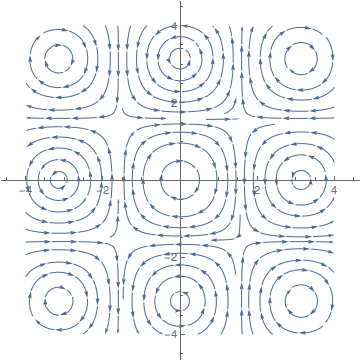
\includegraphics[scale=0.60]{./_Figures/S121.png}
\end{center}
\hfill\qed

\subsubsection*{Solution to $1c$}
When close to the elliptic fixed points, the ODE system behaves like the system
$$\vct{x}{y}' = \pmat{0}{(-1)^{n + m}}{(-1)^{n + m  + 1}}{0}\vct{x}{y}.$$
Therefore
$$\frac{dy}{dx} = \frac{y'}{x'} = \frac{(-1)^{n + m + 1}x}{(-1)^{n + m}y} = -\frac{x}{y}.$$
Solving this gives $x^{2} + y^{2} = C$ for some constant $C$. Therefore the trajectories
near elliptic fixed points are circles and so have period $2\pi$.

On the other hand, when close to hyperbolic fixed points, the ODE system behaves like the system
$$\vct{x}{y}' = \pmat{(-1)^{n + m + 1}}{0}{0}{(-1)^{n + m}}\vct{x}{y}.$$
Therefore
$$\frac{dy}{dx} = \frac{y'}{x'} = \frac{(-1)^{n + m}y}{(-1)^{n + m + 1}x} = -\frac{y}{x}.$$
Solving this gives $xy = C$ for some constant $C$. Therefore as we get arbitrarily close to
a hyperbolic fixed point, we never return and so the period is infinite (we get sent
to another hyperbolic fixed point).
\hfill\qed

\subsection*{Solution to Spring 2012, \#2}\label{s122}

\subsubsection*{Solution to $2a$}
There's probably a typo in the initial conditions. It should probably read
$$ u(x,0) = \frac{\d u}{\d t} (x,0) = 0 $$
as opposed to a partial derivative with respect to $x$.

With this in mind, the solution to the inhomogeneous wave equation comes directly from applying Duhamel's principle, which yields
$$ u(x,t) = \frac{1}{2} \int_0^t \int_{x-(t-s)}^{x+(t-s)} f(y,s) \, dy ds $$ \hfill\qed

\subsubsection*{Solution to $2b$}
\begin{rem}
This problem is a bit confusing since $\Delta$ is a triangle which looks like it depends on inputs $x, t$.
To make our analysis clear, we will assume for the rest of this problem $\Delta$ is a given fixed triangle with vertices that
will not depend on the inputs of any functions that appear in the problem
(for concreteness, we can take $\Delta$ to be, for example, the triangle with vertices $(1, 1), (0, 0)$, and $(2, 0)$). \hfill\qed
\end{rem}

With the above remark in mind, we now solve the problem. Using Duhamel's principle, we can write the solution to the PDE in implicit form:
$$u(x,t) =  \frac{1}{2} \int_0^t \int_{x-(t-s)}^{x+(t-s)} f(y,s) - a(y,s) u_s(y,s) - b(y,s) u_y (y,s) - c(y,s) u(y,s) \, dy ds $$
Hence, a solution to the PDE is a fixed point of the operator
$$ F(\varphi)(x,t) := \frac{1}{2}  \int_0^t \int_{x-(t-s)}^{x+(t-s)} f(y,s) - a(y,s) \varphi_s(y,s) - b(y,s) \varphi_y (y,s) - c(y,s) \varphi (y,s) \, dy ds $$
where $\varphi \in \text{BC}^{1,1} (\R \times (0,\infty) \to \R)$, the set of bounded continuous functions with bounded continuous first derivatives in both variables from $\R \times (0,\infty) \to \R$, which is a complete metric space under the norm defined by
$$ \|u\| :=  \|u(x,t)\|_{\infty} + \left| \left| \frac{\d u}{\d x} (x,t) \right| \right|_{\infty} + \left| \left| \frac{\d u}{\d t} (x,t) \right| \right|_{\infty} $$
where $\| \cdot \|_{\infty}$ is the sup norm. Now, define $h_{\varphi}(y,s) := f(y,s) - a(y,s) u_s(y,s) - b(y,s) u_y (y,s) - c(y,s) u(y,s)$, which is the integrand of the functional defined above. Before we prove that $F$ is a contraction mapping, observe, by the fundamental theorem of calculus,
$$ \frac{\d F}{\d x}(\varphi)(x,t) = \frac{1}{2} \int_0^t h_{\varphi}(x+(t-s),s) - h_{\varphi}(x-(t-s),s) \, ds $$
$$ \frac{\d F}{\d t}(\varphi)(x,t) = \frac{1}{2} \int_0^t h_{\varphi} (x+(t-s),s) + h_{\varphi}(x-(t-s),s) \, ds $$
Define  $C := \max \{ \|a(x,t)\|_{0,\Delta}, \|b(x,t)\|_{0,\Delta}, \|c(x,t)\|_{0,\Delta}\}$. Let $0 < t < T$, where we choose $T < \min \left\{ 2, \frac{1}{6(1+C)} \right\}$. We compute
\begin{align}
\nonumber \|F(\varphi)\| &\leq \frac{1}{2}t^2(  \|f\|_{0,\Delta} + C \|\varphi\|) + 2t( \|f\|_{0,\Delta} + C \|\varphi\|)   \\
\nonumber &< \frac{1}{2}T^2 + 2T(\|f\|_{0,\Delta} + C \|\varphi\|) \\
\label{s12bound} &< \frac{1}{2(1+C)} (\|f\|_{0,\Delta} + C \|\varphi\|)
\end{align}
Define $V := \{ \varphi \in \text{BC}^{1,1} (\R \times (0,\infty) \to \R) \, : \, \|\varphi\| \leq \|f\|_{0,\Delta} \}$. Since $V$ is a closed subset of $\text{BC}^{1,1} (\R \times (0,\infty) \to \R)$, $V$ is complete. We will now show that $F : V \to V$ and that $F$ is a contraction on $V$. In other words, we will show $F(\varphi) \in V$ for all $\varphi \in V$, and for any $\varphi, \phi \in V$, $\|F(\varphi) - F(\phi)\|_{\infty} \leq \alpha \|\varphi-\phi\|_{\infty}$ for some $\alpha \in [0,1)$.

\vspace{0.2cm}

First, we show that $F(\varphi) \in V$ for all $\varphi \in V$. By \eqref{s12bound},
$$\|F(\varphi)\| < \frac{1}{2(1+C)} (\|f\|_{0,\Delta} + C \|f\|_{0,\Delta}) = \frac{1}{2} \|f\|_{0,\Delta} \leq \|f\|_{0,\Delta} $$
Thus, $F(\varphi) \in V$ for all $\varphi \in V$. Next, let $\varphi, \phi \in V$. Then,
\begin{align*}
	\|F(\varphi) - F(\phi)\| &= \frac{1}{2} \left| \left| \int_0^t \int_{x-(t-s)}^{x+(t-s)} h_{\varphi}(y,s) - h_{\phi}(y,s) \, dy ds \right| \right|  \\
	&\leq \frac{1}{2} t^2 C \| \varphi - \phi\| \\
	&< \frac{1}{6} \|\varphi-\phi\|
\end{align*}
Thus, $F$ is a contraction on $V$. Therefore, there exists a unique fixed point in $V$. Since fixed points of $F$ are solutions to the PDE, there exists a unique solution to the PDE if $T$ is chosen sufficiently small. Also, since $f, a, b$, and $c$ are all smooth functions, the solution will be as well.

\vspace{0.4cm}

To show the estimate, we notice
\begin{align*}
	\|u\|_{1,\Delta} &= \|F(u)\|_{1,\Delta} \\
	&= \max_{(y,\tau) \in \Delta} \left( |F(u)| + \left| \frac{\d F}{\d x}(u) \right| + \left| \frac{\d F}{\d t}(u) \right| \right) \\
	&\leq \|F(u)\|_{\infty} + \left| \left| \frac{\d F}{\d x}(u) \right| \right|_{\infty} + \left| \left| \frac{\d F}{\d t}(u) \right| \right|_{\infty} \\
	&\leq \frac{1}{2} t^2 (\|f\|_{0,\Delta} + C \|u\| ) + 2t (\|f\|_{0,\Delta} + C \|u\|) \\
	&= \left( \frac{1}{2} t^2 + 2t \right) (\|f\|_{0,\Delta} + C\|u\|)
\end{align*}
Since $u \in V$, we have
$$ \|u\|_{1,\Delta} \leq \left( \frac{1}{2} t^2 + 2t \right) (\|f\|_{0,\Delta} + C\|f\|_{0,\Delta}) $$
Because we chose $t$ such that $t \leq \min \left\{ 2, \frac{1}{6(1+C)} \right\}$, we have
\begin{align*}
\|u\|_{1,\Delta} &\leq 3t (1+C)\|f\|_{0,\Delta}\\
&\leq \frac{1}{2} \|f\|_{0,\Delta}
\end{align*}
Therefore, the estimate holds.
\hfill\qed

\subsection*{Solution to Spring 2012, \#3}\label{s123}
\subsubsection*{Solution to $3a$}
We have $-sU' + U^{2}U' = \vep U''$ which can be written as $-sU' + (\frac{1}{3}U^{3})' = \vep U''.$
Integrating both sides gives
$$-sU + \frac{1}{3}U^{3} = \vep U' + C_{1}$$
for some constant $C_{1}$.
\hfill\qed

\subsubsection*{Solution to $3b$}
Since $u(+\infty) = U_{R}$ and $u(-\infty) = U_{L}$,
$$-sU_{R} + \frac{1}{3}U_{R}^{3} = C_{1}$$
and
$$-sU_{L} + \frac{1}{3}U_{L}^{3} = C_{1}.$$
Therefore
$$-sU_{R} + sU_{L} + \frac{1}{3}U_{R}^{3} - \frac{1}{3}U_{L}^{3} = 0.$$
Factoring out a $U_{R} - U_{L}$ (which is nonzero) shows that
$$s = \frac{1}{3}(U_{R}^{2} + U_{R}U_{L} + U_{L}^{2})$$ and hence
$$C_{1} = -sU_{R} + \frac{1}{3}U_{R}^{3} = -\frac{1}{3}U_{R}^{2}U_{L} - \frac{1}{3}U_{L}^{2}U_{R}.$$
Since $-sU + \frac{1}{3}U^{3} = \vep U' + C_{1}$,
$-3sU + U^{3} = 3\vep U' + 3C_{1}$ and hence
$$-(U_{R}^{2} + U_{R}U_{L} + U_{L}^{2})U + U^{3} = 3\vep U' - U_{R}^{2}U_{L} - U_{L}^{2}U_{R}.$$
Isolating the $3\vep U'$ terms yields that
$$3\vep U' = (U - U_{R})(U - U_{L})(U + U_{L} + U_{R}).$$
Thus $U$ can be solved for using partial fraction decomposition. Suppose we had $A, B, C$ such that
\begin{align}\label{s123beq1}
\frac{1}{(U - U_{R})(U - U_{L})(U + U_{L} + U_{R})} = \frac{A}{U - U_{R}} + \frac{B}{U - U_{R}} + \frac{C}{U + U_{L} + U_{R}}.
\end{align}
Then
$$A\log|U - U_{R}| + B\log|U - U_{L}| + C\log|U + U_{L} + U_{R}| = \frac{1}{3\vep}s + \wt{C}$$
for some constant $\wt{C}$ (here we have used $\log$ to denote natural log). Thus as long as we can find $A, B, C$ we have a
solution. We have
\begin{align*}
1 = A(U - U_{L})(U + U_{L} + U_{R}) + B(U - U_{R})(U + U_{L} + U_{R}) + C(U - U_{L})(U - U_{R}
\end{align*}
for all $U$. Therefore
\begin{align*}
B(U_{L} - U_{R})(2U_{L} + U_{R}) &= 1\\
A(U_{R} - U_{L})(2U_{R} + U_{L}) & = 1\\
C(-2U_{L} - U_{R})(-2U_{R} - U_{L}) &= 1.
\end{align*}
Thus $A, B, C$ exist if $U_{L} - U_{R} \neq 0$, $2U_{L} + U_{R} \neq 0$, and $2U_{R} + U_{L} \neq 0$.
\hfill\qed

\subsection*{Solution to Spring 2012, \#4}\label{s124}
We will write $X \lsm Y$ if there exists
a positive constant $C$ such that $X \leq CY$. We will write $X \lsm_{f} Y$ if there exists a positive constant $C_{f}$ depending
only on $f$ such that $X \leq C_{f}Y$.
\subsubsection*{Solution to $4a$}
This is similar to the proof of the fundamental solution for the Laplacian. Let $L:= \Delta + k^{2}U$ and $u(x) = \int_{\R^{3}}E(y)f(x - y)\, dy$.
We want to show that $Lu(x) = -f(x)$. We have
\begin{align*}
Lu(x) = \int_{\R^{3}\bs B(0, \vep)}E(y)Lf(x - y)\, dy + \int_{B(0, \vep)}E(y)Lf(x - y)\, dy.
\end{align*}
Observe that
\begin{align*}
\abb{\int_{B(0, \vep)}\frac{e^{ik|y|}}{4\pi|y|}(\Delta_{x}f(x - y) + k^{2}f(x - y))\, dy} \lsm_{f}\int_{B(0, \vep)}\frac{1}{|y|}\, dy \lsm_{f}\int_{0}^{\vep}\frac{1}{r}r^{2}\, dr\lsm_{f} \vep^{2} \rightarrow 0
\end{align*}
as $\vep \rightarrow 0$. Furthermore,
\begin{align*}
\int_{\R^{3}\bs B(0, \vep)}E(y)Lf(x - y)\, dy = \int_{\R^{3}\bs B(0, \vep)}E(y)\Delta_{x}f(x - y)\, dy + \int_{\R^{3}\bs B(0, \vep)}E(y)k^{2}f(x - y)\, dy.
\end{align*}
We have
\begin{align*}
&\int_{\R^{3}\bs B(0, \vep)}E(y)\Delta_{x}f(x - y)\, dy= \int_{\R^{3}\bs B(0, \vep)}E(y)\Delta_{y}f(x - y)\, dy\\
&\quad= -\int_{\R^{3}\bs B(0, \vep)}\nabla E(y) \cdot \nabla_{y}f(x - y)\, dy + \int_{\pr B(0, \vep)}\frac{\pr f}{\pr\nu}(x - y)E(y)\, d\sigma_{y}\\
&\quad= \int_{\R^{3}\bs B(0, \vep)}\Delta E(y)f(x - y)\, dy - \int_{\pr B(0, \vep)}\frac{\pr E}{\pr \nu}(y)f(x - y)\, d\sigma_{y} + \int_{\pr B(0, \vep)}\frac{\pr f}{\pr\nu}(x - y)E(y)\, d\sigma_{y}
\end{align*}
where $\nu$ is the inner normal for $B(0, \vep)$ (which is the outer normal for $\R^{3}\bs B(0, \vep)$.
Since $\Delta E + k^{2}E = 0$ away from $0$,
\begin{align*}
\int_{\R^{3}\bs B(0, \vep)}E(y)Lf(x - y)\, dy = \int_{\pr B(0, \vep)}\frac{\pr f}{\pr \nu}(x - y)E(y) - \frac{\pr E}{\pr \nu}(y)f(x - y)\, d\sigma_{y}.
\end{align*}
Notice that
\begin{align*}
\abb{\int_{\pr B(0, \vep)}\frac{\pr f}{\pr \nu}(x - y)E(y)\, d\sigma_{y}} \lsm_{f} \int_{\pr B(0, \vep)}\frac{1}{\vep}\, d\sigma_{y} \lsm_{f} \vep \rightarrow 0
\end{align*}\
as $\vep \rightarrow 0$. Finally observe that as $\pr_{j}E = \frac{1}{4\pi}e^{ik|x|}(\frac{ikx_{j}}{|x|^{2}} - \frac{x_{j}}{|x|^{3}})$,
$$\nabla E(x) = \frac{e^{ik|x|}}{4\pi}\bigg(\frac{ikx}{|x|^{2}} - \frac{x}{|x|^{3}}\bigg).$$
Since $\nu$ is the inner normal for $B(0, \vep)$, $\nu = -x/|x|$ and hence
$$\frac{\pr E}{\pr \nu}(x) = \nu \cdot \nabla E = -\frac{e^{ik|x|}}{4\pi}\bigg(\frac{ik}{|x|} - \frac{1}{|x|^{2}}\bigg).$$
Thus
\begin{equation}
\begin{aligned}\label{s124eq1}
-\int_{\pr B(0, \vep)}\frac{\pr E}{\pr \nu}(y)f(x - y)\, d\sigma_{y}&= \int_{\pr B(0, \vep)}\frac{e^{ik\vep}}{4\pi}\bigg(\frac{ik}{\vep} - \frac{1}{\vep^{2}}\bigg)f(x -y)\, d\sigma_{y}\\&= \frac{ik\vep e^{ik\vep}}{4\pi \vep^{2}}\int_{\pr B(0, \vep)}f(x - y)\, d\sigma_{y} - \frac{e^{ik\vep}}{4\pi \vep^{2}}\int_{\pr B(0, \vep)}f(x - y)\, d\sigma_{y}.
\end{aligned}
\end{equation}
Since
$$\frac{1}{4\pi\vep^{2}}\int_{\pr B(0, \vep)}f(x - y)\, d\sigma_{y} \rightarrow f(x)$$
as $\vep \rightarrow 0$, it follows that the right hand side of \eqref{s124eq1} tends to $-f(x)$ as $\vep \rightarrow 0$. Therefore $Lu = -f$ as desired.
\hfill\qed

\subsubsection*{Solution to $4b$}
Integration by parts yields
\begin{align*}
\int_{\pr B(0, R)}\frac{\pr u}{\pr \nu}E(x_{0} - y) &- \frac{\pr E(x_{0} -y)}{\pr \nu}u\, d\sigma_{y}\\
&= \int_{B(0, R)}\Delta u E(x_{0} - y)\, dy - \int_{B(0, R)}u\Delta E(x_{0} - y)\, dy\\
&= \int_{B(0, R)}E(x_{0} - y)(\Delta u + k^{2}u) - u(\Delta E(x_{0} - y) + k^{2}E(x_{0} - y))\, dy\\
&= -\int_{B(0, R)}u(-\delta (x_{0} - y))\, dy = u(x_{0}).
\end{align*}
\hfill\qed

\subsubsection*{Solution to $4c$}
Fix arbitrary $x_{0}$ and let $R$ be such that $R > |x_{0}|$. Then
$$u(x_{0}) = \int_{\pr B(0, 2R)}\frac{\pr u}{\pr \nu}E(x_{0} - y) - u\frac{\pr E(x_{0} - y)}{\pr \nu}\, d\sigma_{y}.$$
Note that
\begin{align*}
\frac{\pr E(x_{0} - y)}{\pr \nu} = \nu \cdot \nabla(E(x_{0} - y)) = -\nu \cdot (\nabla E)(x_{0} - y) = \frac{e^{ik|x_{0} - y|}}{4\pi}\bigg(\frac{ik}{|x_{0} - y|} - \frac{1}{|x_{0} - y|^{2}}\bigg)
\end{align*}
and hence
\begin{align*}
u(x_{0}) &= \int_{\pr B(0, 2R)}(o(1/R) + iku)E(x_{0} - y) - u\frac{e^{ik|x_{0} - y|}}{4\pi}\bigg(\frac{ik}{|x_{0} - y|} - \frac{1}{|x_{0} - y|^{2}}\bigg)\, d\sigma_{y}\\
&=\int_{\pr B(0, 2R)}o(\frac{1}{R})E(x_{0} - y) + O(\frac{1}{R})\frac{e^{ik(x_{0} - y)}}{4\pi|x_{0} - y|^{2}}\, d\sigma_{y}.
\end{align*}
Thus
\begin{align*}
|u(x_{0})| &\lsm \int_{\pr B(0, 2R)}o(\frac{1}{R})\frac{1}{|x_{0} - y|} + O(\frac{1}{R})\frac{1}{|x_{0} - y|^{2}}\, d\sigma_{y}\\
&\lsm \int_{\pr B(0, 2R)}o(\frac{1}{R})\frac{1}{R} + O(\frac{1}{R})\frac{1}{R^{2}}\, d\sigma_{y} \lsm o(\frac{1}{R})R + O(\frac{1}{R}) \rightarrow 0
\end{align*}
as $R \rightarrow \infty$. Therefore since $x_{0}$ was arbitrary, $u \equiv 0$.
\hfill\qed

\subsection*{Solution to Spring 2012, \#5}\label{s125}
We will assume that $\beta$ does not vanish on $\pr\Om$ and $\pr\Om$ is sufficiently smooth.
\subsubsection*{Solution to $5a$}
Integration by parts yields that
\begin{align*}
\int_{\Om}v_{x_{k}}\beta(x)u_{x_{k}}\, dx = -\int_{\Om}v(\beta(x)u_{x_{k}})_{x_{k}}\, dx + \int_{\pr\Om}v\beta(x)u_{x_{k}}\nu^{k}\, d\sigma.
\end{align*}
Thus
\begin{align*}
\int_{\Om}\nabla v\cdot (\beta\nabla u)\, dx = -\int_{\Om}v\nabla \cdot (\beta\nabla u)\, dx + \int_{\pr\Om}v\beta\frac{\pr u}{\pr \nu}\, d\sigma.
\end{align*}
We have
\begin{equation}
\begin{aligned}\label{s125eq1}
-\int_{\Om}v\nabla \cdot (\beta \nabla u)\, dx &- \int_{\Om}vf \, dx+ \int_{\pr\Om}\ld v\, d\sigma\\
&+ \int_{\pr\Om}v\beta \frac{\pr u}{\pr \nu}\, d\sigma + \int_{\pr\Om}\mu u \, d\sigma- \int_{\pr \Om}\mu g\, d\sigma  = 0.
\end{aligned}
\end{equation}
Taking $\mu = 0$ and arbitrary $v \in H_{0}^{1}(\Om)$ in \eqref{s125eq1} yields that
$$-\nabla \cdot (\beta \nabla u) = f$$ in $\Om$. Then from \eqref{s125eq1} it follows that for all $v \in H^{1}(\Om)$,
\begin{align}\label{s125eq2}
\int_{\pr\Om}v(\ld + \beta \frac{\pr u}{\pr \nu})\, d\sigma + \int_{\pr\Om}\mu(u - g)\, d\sigma = 0.
\end{align}
Next take $\mu = 0$ in \eqref{s125eq2}. Since $v \in H^{1}(\Om)$ is arbitrary, we have
$$\beta \frac{\pr u}{\pr\nu} = -\ld$$ on $\pr\Om$. Finally, taking $v \in H_{0}^{1}(\Om)$ in \eqref{s125eq2} and using arbitrariness
of $\mu$ shows $u = g$ on $\pr\Om$. Therefore $u$ is the solution of the Dirichlet problem
\begin{align*}
\begin{cases}
-\nabla \cdot (\beta\nabla u) = f & \text{ in } \Om\\
u = g & \text{ on }\pr\Om\\
\beta\nabla u \cdot \nu =-\lambda & \text{ on } \pr\Om.
\end{cases}
\end{align*}
\hfill\qed

\subsubsection*{Solution to $5b$}
We have $\beta(\pr u/\pr\nu) = \beta(\pr w/\pr \nu)$ on $\pr\Om$. Therefore $\beta(\frac{\pr u}{\pr \nu} - \frac{\pr w}{\pr\nu}) = 0$
on $\pr\Om$. If we assume that $\beta$ does not vanish on $\pr\Om$, then $\nabla u \cdot \nu = \nabla w \cdot \nu$ on $\pr\Om$.
Therefore $\nabla u = \nabla w$ on $\pr\Om$ which implies that $w = g + c$ for some $c$ on $\pr\Om$.
\hfill\qed

\subsection*{Solution to Spring 2012, \#6}\label{s126}

\subsubsection*{Solution to $6a$}

Before starting, note that we are looking for the classical/strong solution to the PDE. This means shocks cannot occur, which is why the problem says that the solution can only be defined for some $x$ and $t$.

\vspace{0.4cm}

We use method of characteristics to obtain the following ODEs:
\begin{equation}
	\label{s126eq1} \dot{t}(s) = 1, \quad t(0) = 0
\end{equation}
\begin{equation}
	\label{s126eq2} \dot{x}(s) = z(s), \quad x(0) = x_0
\end{equation}
\begin{equation}
	\label{s126eq3} \dot{z}(s) = 0, \quad z(0) = x_0^2
\end{equation}
Solving \eqref{s126eq1} and \eqref{s126eq3} yields
$$ t(s) = s, \quad \text{and} \quad z(t) = x_0^2 $$
respectively. Then, solving \eqref{s126eq2} yields
\begin{equation}
	\label{s126eq4} x(t) = x_0^2 t + x_0
\end{equation}
Solving \eqref{s126eq4} for $x_0$ will gives
$$ x_0 = \frac{-1 \pm \sqrt{1+4xt}}{2t} $$
In order to determine which sign we pick to define $x_0$, we examine the limit as $t \to 0^+$ of $x_0$. Note that
$$ \lim_{t \to 0^+}  \frac{-1 + \sqrt{1+4xt}}{2t} = \lim_{t \to 0^+} \frac{x}{\sqrt{1+4xt}} = x \quad \text{and} \quad \lim_{t \to 0^+} \frac{-1 - \sqrt{1+4xt}}{2t} = -\infty $$
The first case is the one that we want, so we have
$$ x_0 = \frac{-1 + \sqrt{1+4xt}}{2t} $$
Now, we'll determine for what $x$ and $t$ will we have a strong solution. Consider two characteristics that start at $x=a \geq 0$ and $x=b \geq 0$, namely the characteristics $x = a^2 t + a$ and $ x = b^2 t + b$, respectively. These characteristics crash at $(x,t) = \left( \frac{ab}{a+b}, \frac{-1}{a+b} \right)$, which we can ignore because $t = -1/(a+b) < 0$. Thus, our solution will be defined on at least the set $\{(x,t) \, | \, x \geq 0, t > 0 \}$.

\vspace{0.4cm}

Now, consider the characteristic starting at $x=a < 0$, which will be $x = a^2 t + a$. Because of the slopes of the characteristics that start on the negative $x$-axis, the characteristic $x = a^2t + a$ will crash into another characteristics that starts immediately to the left or right of $a$. From our work above, we already know when and where characteristics crash, so with $a$ fixed, let's send $b$ to $a$ to see where and when the characteristics crash:
$$ x = \lim_{b \to a} \frac{ab}{a+b} = \frac{a}{2}, \quad \text{and} \quad t = \lim_{b \to a} \frac{-1}{a+b} = \frac{-1}{2a} $$
Putting these two expressions together yields
$$t = \frac{-1}{4x} $$
This implies that characteristics that start right next to each other on the negative $x$-axis will crash on the contour $4xt + 1 = 0$. Thus, we have for our strong solution
$$ u(x,t) = \frac{1 + 2xt - \sqrt{1+4xt}}{2t^2} $$
for $x  > -\frac{1}{4t}$ and $t > 0$. Note that $\lim_{t \to 0^+} u(x,t) = x^2$, so this choice of $u$ satisfies the initial condition. \qed


\subsubsection*{Solution to $6b$}
$$ u_x(x,t) = \frac{1}{t} \left( 1 - \frac{1}{\sqrt{1+4xt}} \right) $$
Hence, the magnitude of the derivative of the strong solution becomes infinite when $1+4xt = 0$. In other words, the magnitude of the derivative of our strong solution blows up as we approach the left-hand side boundary of the domain for which our strong solution is defined. This makes sense because that's where all of the characteristics crash. \qed



\subsubsection*{Solution to $6c$}

Recall that, from our work above, the following determines our solution:
$$ x(t) = u_0(x_0) t + x_0, \quad \text{and} \quad z(t) = u_0(x_0) $$
Hence, with our new initial condition, we know that
$$ u(x,t) = \frac{1}{4} \quad \text{when} \quad x - \frac{1}{4} t < -\frac{1}{2} \quad \Leftrightarrow \quad t > 4x+2$$
and
$$ u(x,t) = \frac{1}{4} \quad \text{when} \quad x - \frac{1}{4} t > \frac{1}{2} \quad \Leftrightarrow \quad t < 4x-2$$
This wasn't explicitly stated above, but we always have $t > 0$. Based on our work above, we also know that
$$ u(x,t) = \frac{1 + 2xt - \sqrt{1+4xt}}{2t^2} $$
for $x_0 \in [0,1/2)$, and no characteristics that start in the interval $[0,1/2)$ will crash with the characteristics that start in the interval $(1/2, \infty)$. Hence, everything boils down to what happens when characteristics start in the interval $(-1/2,0)$.

\vspace{0.4cm}

Earlier, we discovered that characteristics that start on the negative $x$-axis will crash along the contour $1+4xt=0$. Because $t=4x+2$ is a characteristic that starts at $x = -1/2$ for initial data $u_0(x) = x^2$, all we need to do is figure out when this line intersects the contour $1+4xt=0$. Some straightforward algebra yields the point $(x,t) = (-1/4, 1)$. Hence, the ODE that describes the trajectory of the shock is
$$ \frac{ \frac{1}{2} \left[ \left( \frac{1}{4} \right)^2 - \left( u_r \right)^2 \right]}{\frac{1}{4} - u_r} = \dot{x}(t), \quad x(1) = -\frac{1}{4}, \quad \text{where} \quad u_r = \frac{1 + 2xt - \sqrt{1+4xt}}{2t^2}. $$ \qed

\subsection*{Solution to Spring 2012, \#7}\label{s127}
Let
$$\phi(r) := \frac{1}{2\pi r}\int_{\pr B(x, r)}u(y)\, d\sigma_{y} = \frac{1}{2\pi}\int_{\pr B(0, 1)}u(x + ry)\, d\sigma_{y}.$$
We have
\begin{align*}
\phi'(r) = \frac{1}{2\pi}\int_{\pr B(0, 1)}\nabla u(x + ry)\cdot y\, d\sigma_{y} = \frac{1}{2\pi r}\int_{\pr B(x, r)}\nabla u(z) \cdot \frac{z - x}{r}\, d\sigma_{z}.
\end{align*}
Since the outer unit normal for $\pr B(x, r)$ is $(z - x)/r$, we have $\nabla u(z) \cdot (\frac{z - x}{r}) = \frac{\pr u}{\pr \nu}$.
Thus
$$\phi'(r) = \frac{1}{2\pi r}\int_{\pr B(x, r)}\frac{\pr u}{\pr \nu}\, d\sigma_{z} = \frac{1}{2\pi r}\int_{B(x, r)}\Delta u\, dz > 0.$$
Therefore $\phi$ is an increasing function of $r$. It follows that for any $\vep > 0$,
$$u(x) = \lim_{r\rightarrow 0}\frac{1}{2\pi r}\int_{\pr B(x, r)}u(y)\, d\sigma_{y} = \lim_{r \rightarrow 0}\phi(r) \leq \phi(\vep) = \frac{1}{2\pi \vep}\int_{\pr B(x, \vep)}u(y)\, d\sigma_{y}.$$
\hfill\qed

\subsection*{Solution to Spring 2012, \#8}\label{s128}
We use separation of variables to find all bounded solutions. Suppose $u(x,y) = X(x)Y(y)$. Plugging this into the PDE yields
\begin{align*}
	 X''(x)Y(y) + X(x)Y''(y) + k^2 X(x)Y(y) = 0 \quad &\implies \quad \frac{X''(x)}{X(x)} + \frac{Y''(y)}{Y(y)} + k^2 = 0 \\
	 &\implies \quad  \frac{X''(x)}{X(x)} + k^2 = -  \frac{Y''(y)}{Y(y)} = \lambda
\end{align*}
Hence, we must solve the following ODEs:
$$ X''(x) + (k^2 - \lambda) X(x) = 0, \quad \text{and} \quad Y''(y) + \lambda Y(y) = 0 $$
After examining the ODE for $x$, it becomes apparent that we require $|\lambda| < k^2$. If $|\lambda| \geq k^2$, then we only have the zero solution. Taking $|\lambda| < k^2$, we have
$$ X(x) = A \sin(\sqrt{k^2 - \lambda} x) + B \cos (\sqrt{k^2 - \lambda} x) $$
Applying the boundary conditions, we get $B = 0$ and
$$ \sqrt{k^2 - \lambda} = n \quad \implies \quad \lambda = k^2 - n^2 $$
for $|n| \leq  k$. Thus, for such $n$,
$$ X_n(x) = A_n \sin (nx) $$
It then follows that the ODE for $y$ is
$$ Y''(y) + (k^2 - n^2) Y(y) = 0 $$
Solving this yields
$$ Y_n(y) = C_n \sin (\sqrt{k^2 - n^2} y) + D_n \cos( \sqrt{k^2 - n^2} y) $$
for $|n| < k$ and
$$ Y_n(y) = D_n $$
for $|n| = k$. Therefore, we have
$$ u(x,y) = \sum_{|n| < k} \sin(nx) \left[ E_n \sin(\sqrt{k^2-n^2} y) + F_n \cos(\sqrt{k^2-n^2} y) \right] + \sum_{|n| = k} G_n \sin(nx) $$
where $E_n, F_n, G_n$ are finite sequences of constants. \qed


\section{Fall 2011}\label{f11}
\noindent The solution to Fall 2011, \#1 is omitted.


\subsection*{Solution to Fall 2011, \#2}
\label{F11Q2}

\subsubsection*{Solution to $2a$}

Since $\nabla \cdot \vB = 0$, our PDE becomes
$$ u_t = \Delta (u^2) + \vB \cdot \nabla u $$
Let $M$ be such that $|u(x,0)| < M$ for all $x$, and let $v := u - M - \epsilon t$. Then, $\nabla v = \nabla u$, $\Delta v = \Delta u$, and $v_t = u_t - \epsilon$. Thus
\begin{align}
\notag v_t &= u_t - \epsilon \\
\notag &= \Delta (u^2) + \vB \cdot \nabla u - \epsilon \\
\notag &= 2(|\nabla u|^2 + u \Delta u) + \vB \cdot \nabla v - \epsilon \\
\label{f112a1} &= 2(|\nabla v|^2 + (v + M + \epsilon t) \Delta v) + \vB \cdot \nabla v - \epsilon
\end{align}
Furthermore, note that $v(x,0) = u(x,0) - M < 0$. We claim that $v(x,t) < 0$ for all $x$ and $t$. Suppose not, which would imply that there exists a first time $t_0$ and a corresponding $x_0$ such that $v(x_0,t_0) = 0$. Since $v(x,t') < 0$ for all $t' < t_0$ and $v(x,t_0) \leq 0$ for all $x$, we must have
$$v_t(x_0,t_0) \geq 0, \quad \text{and} \quad \Delta v(x_0,t_0) \leq 0$$
Thus, by \eqref{f112a1}, we have
$$ 0 \leq v_t (x_0,t_0) = 2(M+\epsilon t_0) \Delta v(x_0,t_0) - \epsilon < 0$$
which is a contradiction. Hence, we must have $v(x,t) < 0 $ for all $x$ and $t$. This implies that
$$ u(x,t) < M + \epsilon t $$
for all $x$ and $t$. Therefore, sending $\epsilon \to 0$ shows
$$ u(x,t) < M $$
for all $x$ and $t$.

In order to show $u$ is bounded below for all $x$ and $t$, we needed to make one extra assumption about $u$. Otherwise, we're not sure how to prove $u$ is bounded below

Fix arbitrary $\delta > 0$. We will show that if $u$ satisfies $u_t = \Delta (u^2) + \vB \cdot \nabla u$ and $u(x,0) < - \delta$, then $u(x,t) \leq 0$ for all $x$ and $t$. Since $u(x,0) < -\delta$ for all $x$, we can choose $\epsilon$ sufficiently small such that $\sup_{x} u(x,0) + \epsilon < 0$. Let
$$ v := u + \lambda \epsilon e^{-\lambda t} $$
where $\lambda$ is to be chosen later. Then,
\begin{align}
\notag v_t &= u_t - \lambda \epsilon e^{-\lambda t} \\
\notag &= -\Delta (u^2) + \vB \cdot \nabla u - \lambda \epsilon e^{-\lambda t} \\
\notag &= -2 (|\nabla u|^2 + u \Delta u) + \vB \cdot \nabla u - \lambda \epsilon e^{-\lambda t} \\
\label{f112a2} &= -2 (|\nabla v|^2 + (v-\epsilon e^{-\lambda t}) \Delta v) + \vB \cdot \nabla v - \lambda \epsilon e^{-\lambda t}
\end{align}
Note $v(x,0) = u(x,0 < 0$. We claim that $v(x,t) < 0$ for all $x$ and $t$. Suppose not, which would imply that there exists a first time $t_0$ and a corresponding $x_0$ such that $v(x_0,t_0) = 0$. Since $v(x,t') < 0$ for all $t' < t_0$ and $v(x,t_0) \leq 0$ for all $x$, we must have
$$v_t(x_0,t_0) \geq 0, \quad \text{and} \quad \Delta v(x_0,t_0) \leq 0$$
Thus, by \eqref{f112a2}, we have
$$ 0 \leq v_t(x_0,t_0) = -2(-\epsilon e^{-\lambda t_0}) \Delta v(x_0,t_0) - \lambda \epsilon e^{-\lambda t_0} < 0$$
for sufficiently large $\lambda$. Thus, we have a contradiction, nad hence,
$$ u(x,t) < -\epsilon e^{-\lambda t} \leq -\epsilon $$
for all $x$ and $t$. Letting $\epsilon \to 0$ shows $u(x,t) \leq 0$ for all $x$ and $t$. Thus, if $u$ satisfies $ u_t = \Delta (u^2) + \vB \cdot \nabla u $ and $u(x,0) > \delta > 0$, then we also have
$$ (-u)_t = -\Delta ((-u)^2) + \vB \cdot \nabla (-u), \quad \text{and} \quad (-u)(x,0) < -\delta $$
Therefore, by our work above, we have $-u(x,t) \leq 0$ for all $x$ and $t$. Thus, $u(x,t) \geq 0$ for all $x$ and $t$, which implies $u$ is bounded below. Again, this result only holds if $u(x,0) > \delta > 0$ for arbitrary $\delta$. \hfill \qed


\subsubsection*{Solution to $2b$}

We consider the equation
$$ u_t = \Delta (u^2) + \nabla \cdot (\vB u) $$
Note that we've relabeled $\theta$ as $u$ and $v$ as $\vB$. We aim to show that if $|\nabla \cdot \vB| \leq M$ for all $x \in \R^n$ and if $u(x,0) \leq 1$, then $u(x,t) \leq e^{Mt}$ for all $t > 0$.

Fix arbitrary $\epsilon > 0$. Let $\eta := e^{Mt}$ and $w := u - \eta - \epsilon e^{\lambda t}$ where $\lambda$ is to be chosen later. Then,
$$ \eta_t = Me^{Mt} \geq (\nabla \cdot \vB) \eta = \nabla \cdot (\vB \eta) $$
Since
$$ \Delta (w^2) = \Delta (u^2) - 2(\eta + \epsilon e^{\lambda t}) \Delta u, \quad \nabla u = \nabla w, \quad \Delta u = \Delta w $$
we have
\begin{align}
\notag w_t &= u_t - \eta_t  - \lambda \epsilon e^{\lambda t} \\
\notag &= \Delta (u^2) + \nabla \cdot (\vB u) - \eta_t - \lambda \epsilon e^{\lambda t} \\
\notag &\leq \Delta (w^2) + 2(\eta + \epsilon e^{\lambda t}) \Delta u + \nabla \cdot (\vB u) - \nabla \cdot (\vB \eta) - \lambda \epsilon e^{\lambda t} \\
\label{f112b1} &= \Delta (w^2) + 2(\eta + \epsilon e^{\lambda t}) \Delta w + (\nabla \cdot \vB)(w + \epsilon e^{\lambda t}) + \vB \cdot \nabla w - \lambda \epsilon e^{\lambda t}
\end{align}
Note $w(x,0) = u(x,0) - 1 - \epsilon < 0$ since $u(x,0) \leq 1$.

We claim that $w(x,t) < 0$ for all $x$ and $t$. Suppose note, which would imply that there exists a first time $t_0$ and a corresponding $x_0$ such that $w(x_0,t_0) = 0$. Since $w(x,t') < 0$ for all $t' < t_0$ and $w(x,t_0) \leq 0$ for all $x$, we must have
$$ w_t(x_0,t_0) \geq 0, \quad \text{and} \quad (\Delta w)(x_0,t_0) \leq 0 $$
Then, by \eqref{f112b1}, we have
$$ w_t(x_0,t_0) \leq \Delta (w^2)(x_0,t_0) + M \epsilon e^{\lambda t_0} - \lambda \epsilon e^{\lambda t_0} $$
Note $\Delta (w^2) = 2 (\left| \nabla w \right|^2 + w \Delta w)$, and thus, $\Delta (w^2)(x_0,t_0) = 0$. Hence,
$$ w_t(x_0,t_0) \leq (M-\lambda)\epsilon e^{\lambda t_0} $$
Choosing $\lambda = 2M$ would yield a contradiction since $w_t(x_0,t_0) \geq 0$. Therefore, no such initial time exists for which $w(x_0,t_0) = 0$, and hence, $w(x,t) < 0$ for all $x$ and $t$.

Finally, we have
$$ u(x,t) < e^{Mt} + \epsilon e^{2Mt} $$
for all $t$. Taking $\epsilon \to 0$ yields
$$ u(x,t) \leq e^{Mt} $$
for all $t>0$. \hfill \qed

\subsection*{Solution to Fall 2011, \#3}
\label{F11Q3}

\subsubsection*{Solution to $3a$}

Taking the Fourier transform, we obtain
$$ \hat{u}_t = -4 \pi^2 |\xi|^2 \hat{u}_t + \hat{u} \quad \implies \quad \hat{u}_t = \frac{\hat{u}}{1 + 4\pi^2|\xi|^2} $$
Since $u \in L^2(\R^n)$ and $\frac{1}{1+4 \pi^@ |\xi|^2} \in L^2(\R^n)$, we have
$$ u_t = u \ast \left[ \frac{1}{1+4 \pi^2 |\xi|^2} \right]^{v} $$
Observe that
\begin{align*}
\left[ \frac{1}{1+4 \pi^2 |\xi|^2} \right]^{v} &= \int_{\R^n} \frac{1}{1+4 \pi^2 |\xi|^2} e^{2 \pi i \xi \cdot x} \, d \xi \\
&= \frac{1}{(2\pi)^n} \int_{\R^n} \frac{1}{1+|\xi|^2} e^{i \xi \cdot x} \, d \xi
\end{align*}
Then, let
$$ G(x) = \frac{1}{(2\pi)^n} \int_{\R^n} \frac{1}{1+|\xi|^2} e^{i \xi \cdot x} \, d \xi $$
so we have
$$ u_t(x,t) = \int_{\R^n} u(y,t) G(x-y) \, dy $$
Finally,
$$ \int_0^t u_t(x,s) \, ds = u(x,t) - u(x,0) = u(x,t) - u_0(x) $$
and thus,
$$ u(x,t) = u_0(x) + \int_0^t \int_{\R^n} u(y,s) G(x-y) \, dy ds $$
\hfill \qed

\subsubsection*{Solution to $3b$}
From our above work, for any $0 \leq s \leq T$,
\begin{align*}
\left| \left| \int_{\R^n} G(x-y) u(y,s) \, dy \right| \right|_{L^2(dx)} &= ||u_t||_{L^2(dx)} = ||\hat{u}_t||_{L^2(d\xi)} \\
&= \left| \left| \frac{\hat{u}}{1 + 4\pi^2|\xi|^2} \right| \right|_{L^2(d\xi)}
\leq ||\hat{u}||_{L^2(d \xi)} = ||u||_{L^2(dx)} = M
\end{align*}
\hfill \qed

\subsubsection*{Solution to $3c$}

Let $F(x,s) := \int_{\R^n} G(x-y) u(y,s) \, dy$. By Minkowski's integral inequality,
$$ \left| \left| \int_0^t \int_{\R^n} G(x-y) u(y,s) \, dy ds \right| \right|_{L^2(dx)} = \left| \left| \int_0^t F(x,s) \, ds \right| \right|_{L^(dx)} \leq \int_0^t ||F(x,s)||_{L^2(dx)} \, dx \leq Mt $$
Then, applying the reverse triangle inequality to the result of part (a) yields
$$ ||u||_{L^2(dx)} \leq ||u_0||_{L^2(dx)} + Mt $$
Thus,
$$ M \geq ||u_0||_{L^2(dx)} \geq \sup_{t \in [0,T]} \left( ||u(\cdot, t)||_{L^2(dx)} - Mt \right) $$
\hfill \qed

\begin{rem}
This is as far as we can go with this problem. Let us know if you have a better solution for part (c).
\end{rem}



\subsection*{Solution to Fall 2011, \#4}
\label{F11Q4}

Let $u$ be a smooth function such that $u_{t} = \Delta(u^{4})$ in $|x| < 1$ and $u = 0$ on $|x| = 1$.

We prove the problem under the two (physically reasonable) assumptions. We will assume that $u(x, 0)$ is bounded for all $|x| \leq 1$
and $u(x, t) \geq 0$ for all $(x, t) \in \{x: |x| \leq 1\} \times [0, \infty)$.
Let $v := (4/3)u^{3}$. Then $v(x, t) \geq 0$ for all $(x, t)$ and
\begin{align}\label{f114eq1}
v_{t} - 3v\Delta v - |\nabla v|^{2} = 0
\end{align}
in $|x| < 1$ and $v = 0$ on $|x| = 1$. Indeed,
\begin{align*}
3v\Delta v + |\nabla v|^{2} = 48 u^{4}\abn{\nabla u}^{2} + 16u^{5}\Delta u = 4u^{2}(12 u^{2}|\nabla u|^{2} + 4u^{3} \Delta u) = 4u^{2}\Delta(u^{4}) = 4u^{2}u_{t} = v_{t}.
%v_{t} = 4u^{2}u_{t} = 4u^{2}\Delta(u^{4})= 4u^{2}(12 u^{2}|\nabla u|^{2} + 4u^{3} \Delta u)= 48 u^{4}\abn{\nabla u}^{2} + 16u^{5}\Delta u =3v\Delta v + |\nabla v|^{2}
\end{align*}
We now prove a maximum principle for \eqref{f114eq1}.
\begin{lemma}\label{F11Q4lem1}
Let $U_{T} := \{x \in \R^{d}: |x| < 1\} \times (0, T]$ and $\Gamma_{T} := \ov{U}_{T} \bs U_{T}$.
Let $v$ be as above. Then for every $T > 0$, $\max_{\ov{U}_{T}}v = \max_{\Gamma_{T}}v.$
\end{lemma}
\begin{proof}
Fix an arbitrary $T > 0$. For every $\vep > 0$, let $v_{\vep}(x, t) := v(x, t) + \vep e^{-At}$ where $A = A(T)$ is to be chosen later.
We compute
\begin{align*}
(v_{\vep})_{t} - 3v_{\vep}\Delta v_{\vep} - \abn{\nabla v_{\vep}}^{2}&= v_{t} - \vep Ae^{-At} - 3(v + \vep e^{-At})\Delta v - |\nabla v|^{2}\\
& = -\vep Ae^{-At} - 3\vep e^{-At}\Delta v = -\vep e^{-At}(A + 3\Delta v).
\end{align*}
If $\nms{\Delta v}_{L^{\infty}(U_{T})} \neq 0$, then we choose $A = 10\nms{\Delta v}_{L^{\infty}(U_{T})}$ and the above calculation shows that
$(v_{\vep})_{t} - 3v_{\vep}\Delta v_{\vep} - \abn{\nabla v_{\vep}}^{2} < 0$.

On the other hand, if $\nms{\Delta v}_{L^{\infty}(U_{T})} = 0$, then we choose $A = 1$. With this choice of $A$, since $\nms{\Delta v}_{L^{\infty}(U_{T})} = 0$
and $\Delta v$ is continuous, $\Delta v = 0$ everywhere in $U_{T}$. Therefore in this case once again, $(v_{\vep})_{t} - 3v_{\vep}\Delta v_{\vep} - \abn{\nabla v_{\vep}}^{2} < 0$.

We now will show that
\begin{align}\label{F11Q4veps}
\max_{\ov{U}_{T}}v_{\vep} = \max_{\Gamma_{T}}v_{\vep}.
\end{align}
Suppose there exists an $(x_{0}, t_{0}) \in U_{T}$
with $v_{\vep}(x_{0}, t_{0}) = \max_{\ov{U}_{T}}v_{\vep}$, such a point exists since $\ov{U}_{T}$ is compact and $v_{\vep}$ is smooth.
Since $v_{\vep}$
attains a maximum at $(x_{0}, t_{0})$, $(v_{\vep})_{t}(x_{0}, t_{0}) \geq 0$ (note that $(v_{\vep})_{t}(x_{0}, t_{0}) = 0$ if $t_{0} < T$, we only get
$\geq 0$ in the case if $t_{0} = T$), $(\nabla v_{\vep})(x_{0}, t_{0}) = 0$, and $\Delta(v_{\vep})(x_{0}, t_{0}) \leq 0$.
Since we assumed $u \geq 0$ everywhere, $v(x_{0}, t_{0}) = (4/3)u(x_{0}, t_{0})^{3}\geq 0$ and hence $v_{\vep}(x_{0}, t_{0}) > 0$.
Therefore at $(x_{0}, t_{0})$, $(v_{\vep})_{t} - 3v_{\vep}\Delta v_{\vep} - \abn{\nabla v_{\vep}}^{2} \geq 0$, a contradiction.
This proves \eqref{F11Q4veps} and letting $\vep \rightarrow 0$ in \eqref{F11Q4veps} completes the proof of the claim.
\end{proof}
For arbitrary $T > 0$, the above lemma implies that
\begin{align*}
\max_{\ov{U}_{T}}v = \max_{\Gamma_{T}}v = \max_{|x| < 1}v(x, 0) < \infty
\end{align*}
where the last equality is because $v = 0$ on $|x| = 1$ and the last inequality is because $v = (4/3)u^{3}$ and we assumed $u(x, 0)$ to be bounded.
Therefore since $T$ was arbitrary, $u$ is bounded above everywhere in $\{x \in \R^{d}: |x| \leq 1\} \times [0, \infty)$.

Let $$E(t) := \int_{|x| \leq 1} u^{5}\, dx.$$ Since $u \geq 0$ for all $(x, t)$, $E(t) \geq 0$ for all $t$. Taking the time derivative yields
$$\dot{E}(t) = 5\int_{|x| \leq 1}u^{4}u_{t}\, dx = 5\int_{|x| \leq 1}u^{4}\Delta (u^{4})\, dx = -5\int_{|x| \leq 1}|\nabla(u^{4})|^{2}\, dx \leq 0$$
where in the third equality we have used that $u = 0$ on $|x| = 1$.

Since $E(0) = \int_{|x| \leq 1}u(x, 0)^{5}\, dx < \infty$
and $E(t)$ is bounded above (since $u$ is bounded above everywhere) and below, there exists some constant $C$ such that $E(t) \rightarrow C$ as $t \rightarrow \infty$.
Therefore $|\nabla(u^{4})|^{2} \rightarrow 0$ as $t \rightarrow \infty$
and hence $u$ tends to a constant as $t \rightarrow \infty$. Since $u = 0$ on $|x| = 1$ for all time, it follows that $u$ vanishes to zero as $t \rightarrow \infty$. \hfill \qed



\subsection*{Solution to Fall 2011, \#5}
\label{F11Q5}

\subsubsection*{Solution to $5a$}

By the method of characteristics, we have
$$
\begin{array}{lll}
\dot{t}(s) = 1, \quad t(0) = 0 & \implies & t(s) = s \\
\dot{x}(s) = f'(z(s)), \quad x(0) = x_0 & \implies & x(s) = x(t) = f'(-x_0)t + x_0 \\
\dot{z}(s) = 0, \quad z(0) = -x_0 & \implies & z(s) = z(t) = -x_0
\end{array}
$$
Hence, implicitly, the solution is $u(x,t) = -r$ where $x = f'(-r)t + r$. Now, we compute
$$ u(x,t) = -r \quad \implies \quad \frac{\d u}{\d x} = -\frac{\d r}{\d x} $$
and
\begin{align*}
x = f'(-r)t + r \quad &\implies \quad 1 = - f''(-r) t \frac{\d r}{\d x} + \frac{\d r}{\d x} \\
&\implies \quad \frac{\d r}{\d x} = \frac{1}{1-f''(-r)t}
\end{align*}
Thus,
$$ \left| \frac{\d u}{\d x} \right| = \frac{1}{|1-f''(-r)t|} $$
Recall $f''(x) > \theta > 0$ for all $x$, which implies that, by time $t = 1/\theta$, $|u_x|$ will have already blown up. Therefore, $|u_x|$ blows up in finite time. \hfill \qed

\subsubsection*{Solution to $5b$}

First, note that this is exactly Theorem 4 in section 3.4.4 in Evans. We're going to take the result from there, but also show a slightly different proof for the case where $u^- < u^+$.

\vspace{0.2cm}

\noindent
Recall, to check that a solution is an entropy solution, we need to check the following:
\begin{enumerate}
\item The solution is indeed a solution to the PDE in its domain of definition

\item The Rankine-Hugoniot condition is satisfied at the shocks

\item The entropy condition is satisfied near the shocks
\end{enumerate}

For the case where $u^- > u^+$, the characteristics crash immediately since $f'' > 0$. Let
$$ u(x,t) := \left\{
\begin{array}{ll}
u^- & \text{if} \,\, x < s(t) \\
u^+ & \text{if} \,\, x > s(t)
\end{array} \right. $$
where
$$ \dot{s}(t) = \frac{f(u^-) - f(u^+)}{u^- - u^+} =: \sigma, \quad s(0) = 0 \quad s(t) = \sigma t $$
Hence,
\begin{equation}
\label{f1151}
u(x,t) := \left\{
\begin{array}{ll}
u^- & \text{if} \,\, \frac{x}{t} < \sigma \\
u^+ & \text{if} \,\, \frac{x}{t} > \sigma
\end{array} \right.
\end{equation}
Note that $u$ satisfies the Rankine-Hugoniot jump condition. Also,
$$ (u^{\pm})_t + (f(u^{\pm}))_x = 0 $$
when $x/t > \sigma$ and $x/t < \sigma$, respectively. Finally, because $u^- > u^+$, the entropy condition is satisfied because $f'' > \theta > 0$. By uniqueness, \eqref{f1151} is the entropy solution when $u^- > u^+$.

\vspace{0.2cm}

If $u^- < u^+$, let
$$ u(x,t) = \left\{
\begin{array}{cc}
u^- & \text{if} \,\, \frac{x}{t} < f'(u^-) \\
G\left( \frac{x}{t} \right) & \text{if} \,\, f'(u^-) < \frac{x}{t} < f'(u^+) \\
u^+ & \text{if} \,\, f'(u^+) < \frac{x}{t}
\end{array} \right. $$
where $G := (f')^{-1}$.
Note that $u$ is continuous! To see this, observe that, along the shock curve $x/t = f'(u^-)$, we have
$$ G\left( \frac{x}{t} \right) = G(f'(u^-)) \quad \implies \quad G\left( \frac{x}{t} \right) = u^- $$
Similarly, along the shock curve $x/t = f'(u^+)$, we have
$$ G\left( \frac{x}{t} \right) = G(f'(u^+)) \quad \implies \quad G(\left( \frac{x}{t} \right) = u^+ $$
Thus, $u$ vacuously satisfies \emph{both} the Rankine-Hugoniot jump condition and the entropy condition. Hence, it remains to check that $u$ satisfies the PDE. Our work in part (a) already shows that in the regions where $u(x,t) = u^{\pm}$, $u$ satisfies the PDE. Observe,
\begin{align*}
\left( G\left( \frac{x}{t} \right) \right)_t + \left( f \left( G \left( \frac{x}{t} \right) \right) \right)_x &= G'\left( \frac{x}{t} \right) \left( -\frac{x}{t^2} \right) + f'\left( G\left( \frac{x}{t} \right) \right) G'\left( \frac{x}{t} \right) \frac{1}{t} \\
&= G'\left( \frac{x}{t} \right) \left( -\frac{x}{t^2} \right) + \frac{x}{t^2} G'\left( \frac{x}{t} \right) \\
&= 0
\end{align*}
Therefore, $u$ is an entropy solution and by uniqueness, it is the entropy solution. \hfill \qed

\subsection*{Solution to \#6}
\label{F11Q6}

\subsubsection*{Solution to $6a$}
Fix $(x_0,t_0)$, and define
$$
K(x_0,t_0) = \left\{ (x,t) \, : \, x_0 - 3t_0 + 3t \leq x \leq x_0 + t_0 - t, \,\, 0 \leq t \leq t_0 \right\}
$$
Furthermore, suppose $u$ and $v$ are solutions to the PDE with the same initial data on the interval $(x_0-3t_0, x_0+t_0)$ and arbitrary initial data elsewhere. Then, $w:= u-v$ satisfies
\begin{gather*}
w_{tt} + 2w_{xt} - 3w_{xx} = 0, \quad x \in \R, \,\, t > 0 \\
w(x,0) = \left\{
\begin{array}{ll}
0 & \text{for} \,\, x \in (x_0-3t_0, x_0+t_0) \\
f(x) & \text{otherwise}
\end{array} \right. \\
w_t(x,0) = \left\{
\begin{array}{ll}
0 & \text{for} \,\, x \in (x_0-3t_0, x_0+t_0) \\
g(x) & \text{otherwise}
\end{array} \right.
\end{gather*}
where $f$ and $g$ are arbitrary functions. Define
$$ E(t) := \frac{1}{2} \int_{x_0 - 3t_0 + 3t}^{x_0 + t_0 - t} w_t^2 + 3w_x^2 \, dx $$
for $0 \leq t \leq t_0$. Then,
\begin{equation}
\label{f1161}
\dot{E}(t) = \int_{x_0 - 3t_0 + 3t}^{x_0 + t_0 - t} w_t w_{tt} + 3 w_x w_{xt} \, dx - \frac{1}{2} (w_t^2 + 3w_x^2) \bigg|_{x = x_0 + t_0 - t} - \frac{3}{2} (w_t^2 + 3w_x^2) \bigg|_{x = x_0 -3t_0 + 3t}
\end{equation}
Applying integration by parts, we have
\begin{align*}
\int_{x_0 - 3t_0 + 3t}^{x_0 + t_0 - t} w_t w_{tt} + 3 w_x w_{xt} \, dx &= \int_{x_0 - 3t_0 + 3t}^{x_0 + t_0 - t} w_t w_{tt} - 3 w_{xx} w_{t} \, dx + 3w_x w_t \bigg|_{x=x_0 - 3t_0 + 3t}^{x=x_0 + t_0 - t} \\
&= \int_{x_0 - 3t_0 + 3t}^{x_0 + t_0 - t} -2 w_{xt} w_t \, dx + 3w_x w_t \bigg|_{x=x_0 - 3t_0 + 3t}^{x=x_0 + t_0 - t}
\end{align*}
where the second equality is from using the PDE. Then, using integration by parts again yields
$$ \int_{x_0 - 3t_0 + 3t}^{x_0 + t_0 - t} -2 w_{xt} w_t \, dx = -2w_t^2 \bigg|_{x=x_0 - 3t_0 + 3t}^{x=x_0 + t_0 - t} + \int_{x_0 - 3t_0 + 3t}^{x_0 + t_0 - t} 2w_{t}w_{xt} \, dx $$
which implies
$$ \int_{x_0 - 3t_0 + 3t}^{x_0 + t_0 - t} -2w_{xt} w_t \, dx = -w_t^2 \bigg|_{x=x_0 - 3t_0 + 3t}^{x=x_0 + t_0 - t} $$
Plugging everything back into \eqref{f1161} yields
\begin{align*}
\dot{E}(t) &= -w_t^2 \bigg|_{x=x_0 - 3t_0 + 3t}^{x=x_0 + t_0 - t} + 3w_x w_t \bigg|_{x=x_0 - 3t_0 + 3t}^{x=x_0 + t_0 - t}- \frac{1}{2} (w_t^2 + 3w_x^2) \bigg|_{x = x_0 + t_0 - t} - \frac{3}{2} (w_t^2 + 3w_x^2) \bigg|_{x = x_0 -3t_0 + 3t} \\
&= \left[ 3w_x w_t -\frac{3}{2} w_t^2 - \frac{3}{2} w_x^2 \right]_{x = x_0 + t_0 - t} +  \left[-3w_x w_t - \frac{1}{2} w_t^2 - \frac{9}{2} w_x^2 \right]_{x = x_0 - 3t_0 + 3t} \\
&= -\frac{3}{2} (w_t - w_x)^2 \bigg|_{x=x_0 + t_0 -t} - \frac{1}{2} (w_t + 3w_x)^2 \bigg|_{x = x_0 - 3t_0 + 3t} \leq 0
\end{align*}
for all $0 \leq t \leq t_0$. Hence, we've shown $E(t) \leq E(0)$. Furthermore, note
$$
E(0) = \frac{1}{2} \int_{x_0 - 3t_0}^{x_0+t_0} w_t(x,0)^2 + 3w_x(x,0)^2 \, dx = 0
$$
so $E(t) = 0$ for all $0 \leq t \leq t_0$. This implies that $w_t \equiv 0$ and $w_x \equiv 0$ in $K(x_0,t_0)$. Putting this together with the fact that $w(x,0) = w_t(x,0) = 0$ on $(x_0-3t_0, x_0+t_0)$, we have $w \equiv 0$ in $K(x_0,t_0)$. Hence, $u \equiv v$ in $K(x_0,t_0)$. Therefore, initial data outside of the interval $(x_0-3t_0,x_0+t_0)$ does not affect the values of the solution in $K(x_0,t_0)$, which includes the point $(x_0,t_0)$. Therefore, the value of the solution at the point $(x_0,t_0)$ depends on at most the values of the initial data in the interval $(x_0-3t_0, x_0+ t_0)$.  \hfill \qed

\subsubsection*{Solution to $6b$}

Suppose $u$ and $v$ are solutions to the PDE with compactly supported initial data. Then $w:=u-v$ satisfies
\begin{gather*}
w_{tt} + 2w_{xt} - 3w_{xx} = 0, \quad x \in \R, \,\, t > 0 \\
w(x,0) = 0 \\
w_t(x,0) = 0
\end{gather*}
Note that, because the initial data is compactly supported, our work in part (a) guarantees that $u$ and $v$ are compactly supported for all time. To see this, notice that if we pick $(x_0,t_0)$ such that the interval $(x_0 - 3t_0, x_0 + t_0)$ is outside the support of the initial data, then the value of the solutions at $(x_0,t_0)$ will be 0. For each $t > 0$, we can always find an $x$ of sufficiently large magnitude such that this happens. Hence, solutions are compactly supported for all time. This then implies that $w$ is compactly supported for all time. Now, define
$$ E(t) = \frac{1}{2} \int_{\R} w_t^2 + 3w_x^2 \, dx $$
We compute, using integration parts along the way,
\begin{align*}
\dot{E}(t) &= \int_{\R} w_t w_{tt} + 3w_x w_{xt} \, dx \\
&=\int_{\R} w_t w_{tt} - 3x_{xx} w_t \, dx \\
&= \int_{\R} -2w_{xt} w_t \, dx
\end{align*}
Because $w$ is compactly supported, the boundary terms vanish. Another application of integration by parts yields
$$ \int_{\R} -2w_{xt} w_t \, dx = \int_{\R} w_{t} w_{xt} \, dx \quad \implies \quad \int_{\R} -2w_{xt} w_t \, dx = 0 $$
Hence, we've shown that $\dot{E}(t) = 0$, which implies that $E(t) = E(0) = 0$ for all time. Thus, $w_t \equiv 0$ and $w_x \equiv 0$ for all time, and because $w(x,0) = w_t(x,0) = 0$, we must have $w \equiv 0$ for all time. Therefore, $u \equiv v$, so solutions to the PDE are unique. \hfill \qed









\subsection*{Solution to Fall 2011, \#7}
\label{F11Q7}

\subsubsection*{Solution to $7a$}
This problem might be missing some assumptions, since, for example, $\vf=\mathbf{0}$ is a counterexample. Thus, we are going to make the assumption that $\vf \not\equiv 0$, and that, at the equilibrium points, $(f_1)_u \neq 0$ and $(f_1)_v \neq 0$.

Consider the Jacobian of $\vf(\vu)$,
$$ J[\vf(\vu)] = \left(
\begin{array}{cc}
(f_1)_u & (f_1)_v \\
(f_2)_u & (f_2)_v
\end{array}
\right)
$$
We aim to show that eigenvalues of this matrix, when evaluated at the equilibrium points, are always of opposite signs, which would then imply that any stationary points of the system must be saddle points. Observe that
\begin{equation}
\label{F117det}
\det(J[\vf(\vu)]) = (f_1)_u (f_2)_v - (f_1)_v (f_2)_u
\end{equation}
Since we have $(f_1)_u = -(f_2)_v$ and $(f_1)_v = (f_2)_u$, \eqref{F117det} becomes
$$ \det(J[\vf(\vu)]) = -\left((f_2)_v \right)^2 - \left((f_2)_u \right)^2 \ $$
Because of our assumptions above, the determinant is negative, implying that the eigenvalues are of opposite signs. Therefore, any equilibrium points are saddle points. \hfill \qed


\subsubsection*{Solution to $7b$}
To show $\vf$ is $C^{\infty}$, we aim to show that both components of $\vf$ are harmonic, and thus smooth. Note that, from our assumptions, we have
$$ (f_1)_u = -(f_2)_v \quad \implies \quad (f_1)_{uu} = -(f_2)_{vu} $$
and
$$ (f_1)_v = (f_2)_u \quad \implies \quad (f_1)_{vv} = (f_2)_{uv} $$
Thus,
$$ \Delta f_1 = (f_1)_{uu} + (f_1)_{vv} = 0 $$
A similar argument would also show $\Delta f_2 = 0$. Therefore, since harmonic functions are smooth, we have that $\vf$ is smooth. \hfill \qed





\subsection*{Solution to Fall 2011, \#8}
\label{F118}

\subsubsection*{Solution to $8a$}

To show that $\lambda > 0$, we multiply the PDE by $u$ and integrate.
\begin{align*}
\lambda \int_{\Omega} u^2 \, dx &= -\int_{\Omega} \Delta u u \, dx \\	
&= \int_{\Omega} |\nabla u|^2 \, dx
\end{align*}
We get the second inequality from integration by parts. Note that the integral over the boundary vanishes because $u$ vanishes on the boundary. Because $u$ is nonzero, both integrals are positive, implying that $\lambda > 0$. \hfill \qed

\subsubsection*{Solution to $8b$}

Define $F(u) := \int_U |Du|^2 \, dx$ and $G(u) := \int_U u^2 \, dx$. Suppose $w \in H^1_0(\Omega)$ minimizes $F$ subject to the constraint $G(w) = 1$,  and let $v \in H_0^1(U)$ be arbitrary. By method of Lagrange multipliers,
$$ F'(w)v = \mu G'(w)v $$
for some $\mu \in \R$, where $F'(w)v$ is the Frechet derivative of $F$ at $w$ in the direction of $v$. We compute
\begin{align*}
F'(w)v &= \lim_{\epsilon \to 0} \frac{1}{\epsilon} \left(F(w+\epsilon v)-F(w)\right) \\
&= \lim_{\epsilon \to 0} \frac{1}{\epsilon} \left( \int_U |Dw+ \epsilon Dv|^2 \, dx - \int_U |Dw|^2 \, dx \right)	\\
&= \lim_{\epsilon \to 0} \frac{1}{\epsilon} \left( \int_U 2\epsilon Dw \cdot Dv + \epsilon^2 |Dv|^2 \, dx \right) \\
&= 2 \int_U Dw \cdot Dv \, dx
\end{align*}
and
\begin{align*}
G'(w)v &= \lim_{\epsilon \to 0} \frac{1}{\epsilon} (G(w + \epsilon v) - G(w)) \\
&= \lim_{\epsilon \to 0} \frac{1}{\epsilon} \left( \int_U (w+\epsilon v)^2 \, dx - \int_U w^2 \, dx \right) \\
&= \lim_{\epsilon \to 0} \frac{1}{\epsilon} \left( \int_U 2 \epsilon wv + \epsilon^2 v^2 \, dx \right) \\
&= 2 \int_U wv \, dx
\end{align*}
Thus, we have
\begin{equation}
\label{f118weak}
	\int_U Dw \cdot Dv \, dx = \mu \int_U wv \, dx
\end{equation}
Since this holds for all $v \in H_0^1(U)$, letting $v=w$ yields
$$ \int_U |Dw|^2 \, dx = \mu \int_U w^2 \, dx \quad \implies \quad \mu = \int_{U} |Dw|^2 \, dx $$
Hence, $\mu$ is the value achieved by the minimizer of $F$ subject to the constraint $G(w)=1$. Now, applying integration by parts to the integral on the left of \eqref{f118weak} yields
$$ -\int_U \Delta w v \, dx = \mu \int_U wv \,dx $$
The integral over the boundary vanishes because $v$ vanishes on the boundary. Therefore, since this holds for all $v \in H_0^1(U)$,
$$ -\Delta w = \mu w $$
Finally, let $\varphi$ be any arbitrary eigenfunction of $-\Delta$ with associated eigenvalue $\gamma$ where $\gamma \neq \mu$. Without loss of generality, we may take $\|\varphi\|_{H^1_0(\Omega)} = 1$. Then,
$$ \mu = \int_U |Dw|^2 \, dx \leq \int_U |D\varphi|^2 \, dx = -\int_U \varphi \Delta \varphi \, dx = \gamma \int_U \varphi^2 \, dx = \gamma $$
Hence, the value achieved by the minimizer is indeed the smallest eigenvalue. \hfill \qed


\section{Spring 2011}\label{s11}
\noindent The solution to Spring 2011, \#2 is omitted.

\subsection*{Solution to Spring 2011, \#1}\label{s111}
We rewrite the system as
\begin{align*}
x' &= y\\
y' &= -kx - ax^{3}.
\end{align*}
Since $\frac{\pr}{\pr x}(y) + \frac{\pr}{\pr y}(-kx - ax^{3}) = 0$, the system is a Hamilitonian
system and hence all equilibrium points are centers or saddles. The Jacobian is
$$J(x, y) = \pmat{0}{1}{-k - 3ax^{2}}{0}.$$
The equilibrium points are
\begin{itemize}
\item $(0, 0)$ if $a \geq 0$
\item $(0, 0)$ and $(\pm \sqrt{-\frac{k}{a}}, 0)$ if $a < 0$.
\end{itemize}
At the equilbrium point $(0, 0)$, $J(0, 0) = \smat{0}{1}{-k}{0}$ which has eigenvalues
$\pm ki$. Therefore since the system is Hamiltonian, $(0, 0)$ is a center (alternatively,
one could prove $(0, 0)$ is a center by solving $\frac{dy}{dx} = \frac{-kx - ax^{3}}{y}$ which
gives a conserved quantity/Lyapunov function. See the solution to Spring 2015, \#8 for more
details). Therefore in the case of a hard spring, we only have a center at $(0, 0)$.
In the case of a soft spring, we have a center at $(0, 0)$ in addition to saddles at
$(\pm \sqrt{-\frac{k}{a}}, 0)$. Indeed,
$$J(\pm \sqrt{-\frac{k}{a}}, 0) = \pmat{0}{1}{2k}{0}.$$
The eigenvalues of this matrix are $\pm\sqrt{2k}$ and hence $(\pm\sqrt{-\frac{k}{a}}, 0)$
are saddles.

If we add a damping term, then for some $b \neq 0$, our system becomes
\begin{align*}
x' &= y\\
y' &= -kx - ax^{3} + by.
\end{align*}
The Jacobian is $$J(x, y) = \pmat{0}{1}{-k - 3ax^{2}}{b}.$$ The equilibrium points are once again
\begin{itemize}
\item $(0, 0)$ if $a > 0$
\item $(0, 0)$ and $(\pm \sqrt{-\frac{k}{a}}, 0)$ if $a < 0$.
\end{itemize}
At $(0, 0)$, $J(0, 0) = \smat{0}{1}{-k}{b}$ which has eigenvalues
$(b \pm \sqrt{b^{2} - 4k})/2$. Thus
\begin{itemize}
\item if $b^{2} - 4k > 0$, then $(0, 0)$ is a saddle
\item if $b^{2} - 4k = 0$, then $(0, 0)$ is an improper node (stable if $b < 0$ and unstable if $b > 0$)
\item if $b^{2} - 4k < 0$, then $(0, 0)$ is a clockwise spiral (since for $\vep > 0$ small, $\smat{0}{1}{-k}{b}\svt{\vep}{0} = \svt{0}{-k}$ and so the spiral points in the clockwise
direction).
\end{itemize}
At $(\pm \sqrt{-\frac{k}{a}}, 0)$,
$J(\pm \sqrt{-\frac{k}{a}}, 0) = \smat{0}{1}{2k}{b}$ which has eigenvalues
$(b \pm \sqrt{b^{2} + 8k})/2$. Therefore $(\pm\sqrt{-\frac{k}{a}}, 0)$
are still saddles.
\hfill\qed

\subsection*{Solution to Spring 2011, \#3}\label{s113}
We present two similar solutions. One in the spirit of the proof of the maximum principle, another using a ``first time" argument.

\vspace{0.25in}

\noindent \textbf{``Maximum Principle" Approach:} Define $w(x,t) := e^{-\lambda t} u(x,t)$, where $\lambda > \max_{x \in \overline{D}} a(x)$. Note that $\lambda$ is well-defined because $a(x)$ is a continuous on a closed and bounded domain set $\overline{D}$.  Because of the initial and boundary conditions on $u$, observe that $w$ vanishes on $\Gamma$ and $w(x,0) \geq 0$ for all $t>0$. Now, suppose $w$ achieves a negative minimum at $(x_0,t_0)$. Note that this must be in the interior of $D \times (0,\infty)$ since $w \geq 0$ on the parabolic boundary. Then,
$$ (w_t - \Delta w)(x_0,t_0) \leq 0$$
However, at the same time,
\begin{align*}
	w_t - \Delta w &= e^{-\lambda t} (u_t - \Delta u - \lambda u) \\
	&= (a(x) - \lambda) w
\end{align*}
so we have
$$ (w_t - \Delta w)(x_0,t_0) = (a(x_0) - \lambda) w(x_0,t_0) > 0 $$
Because of our choice of $\lambda$ above, $a(x) - \lambda < 0$ for all $x \in \overline{D}$. We have reached a contradiction, which implies $w$ will never achieve a negative minimum. Therefore, $w(x,t) \geq 0$ for all $(x,t) \in D \times (0,\infty)$. Finally, because $e^{-\lambda t} > 0$ for all $t$, we also have that $u(x,t) \geq 0$ for all $(x,t) \in D \times (0,\infty)$. \qed

\vspace{0.25in}

\noindent \textbf{``First Time" Approach:} Let $M := \max_{\ov{D}}a(x)$ and $v(x, t) := e^{-(2M + 1)t}u(x, t)$. Then $v_{t} = -(2M + 1)e^{-(2M + 1)t}u + e^{-(2M + 1)t}u_{t}$
Since $u_{t} - \Delta u = a(x)u$, multiplying both sides by $e^{-(2M + 1)t}$ and using our relation between $u_{t}$ and $v_{t}$ yields
that $$v_{t} - \Delta v = (a(x) - 2M - 1)v.$$
\begin{claim}\label{s113cl1}
For every $\vep > 0$, $v(x, t) > -\vep$ for all time.
\end{claim}
\begin{proof}
Fix arbitrary $\vep > 0$. Suppose the claim was false. Then there exists a minimal time $t_{0}$ and a corresponding $x_{0}$ such that $v(x_{0}, t_{0}) = -\vep$. Since
$v(x, 0) = u(x, 0) \geq 0$ and $v(x, t') > -\vep$ for $t' < t_{0}$ and $v(x, t_{0}) \geq -\vep$, we have $v_{t}(x_{0}, t_{0}) \leq 0$ and $(\Delta v)(x_{0}, t_{0}) \geq 0$.
Therefore at $(x_{0}, t_{0})$, $v_{t} - \Delta v \leq 0$. But
$$v_{t}(x_{0}, t_{0}) - (\Delta v)(x_{0}, t_{0}) = (a(x_{0}) - 2M - 1)v(x_{0}, t_{0}) = -\vep(a(x_{0}) - 2M - 1) > 0$$
where in the last inequality we have used how $M$ was defined. This is a contradiction. Therefore no such minimal time exists
and hence $v(x, t) > -\vep$ for all time. This completes the proof of Claim \ref{s113cl1}.
\end{proof}
Thus by the claim, letting $\vep \rightarrow 0$, $v(x, t) \geq 0$ for all time and hence $u \geq 0$ for all time. \hfill\qed

\subsection*{Solution to Spring 2011, \#4}\label{s114}
The equation we want to solve is
\begin{align*}
u_{x}^{2} + u_{x}u_{y} &= 1\\
u(x, 0) &= f(x).
\end{align*}
We use method of characteristics. We have $F(p, q, z, x, y) = p^{2} + pq - 1$. Method of characteristics yields the following system
\begin{align*}
\begin{array}{ll}
 \dot{x} = 2p + q& x(0) = x_{0} \\
 \dot{y} = p& y(0) = 0\\
 \dot{z} = 2p^{2} + 2pq & z(0) = f(x_{0})\\
 \dot{p} = 0 & p(0) = f'(x_{0})\\
 \dot{q} = 0 & q(0) = \frac{1}{f'(x_{0})} - f'(x_{0}).
\end{array}
\end{align*}
The problem is characteristic when $f'(x_{0}) = 0$. We now assume that $f'(x_{0}) \neq 0$. We have
\begin{align*}
p(s) &= f'(x_{0})\\
q(s) &= \frac{1}{f'(x_{0})} - f'(x_{0})\\
y(s) &= f'(x_{0})s.
\end{align*}
Since we have solved for $p(s)$ and $q(s)$, we have
\begin{align*}
\dot{z} = 2p^{2} + 2pq = 2(p^{2} + pq) = 2.
\end{align*}
Thus
$$z(s) = f(x_{0}) + 2s = f(x_{0}) + \frac{y(s)}{f'(x_{0})}.$$
Therefore
\begin{align*}
x(s) &= x_{0} + (2f'(x_{0}) + \frac{1}{f'(x_{0})} - f'(x_{0}))s = x_{0} + (f'(x_{0}) + \frac{1}{f'(x_{0})})s \\
&= x_{0} + (f'(x_{0}) + \frac{1}{f'(x_{0})})\frac{y(s)}{f'(x_{0})} = x_{0} + (1 + \frac{1}{f'(x_{0})^{2}})y(s).
\end{align*}
and hence
$$f'(x_{0})^{2}(x - x_{0}) = f'(x_{0})^{2}y + y.$$
Rearranging this yields that
$$y = f'(x_{0})^{2}(x - x_{0} - y).$$
Let $r(x, y)$ be defined near $(x_{0}, 0)$ by $y = f'(r)^{2}(x - r - y)$, then the solution is
$$u(x,y) = f(r) + \frac{y}{f'(r)}.$$
We now show that there is a unique local solution with $r(x_{0}, 0) = x_{0}$. Let
$$G(x, y, r) := f'(r)^{2}(x - r - y) - y.$$
Then
$$G_{r}(x, y, r) = 2f'(r)f''(r)(x - r - y) - f'(r)^{2}$$
and hence
$$G_{r}(x_{0}, 0, x_{0}) = 2f'(x_{0})f''(x_{0})(x_{0} - x_{0} - 0) - f'(x_{0})^{2} = -f'(x_{0})^{2} \neq 0.$$
Thus by the implicit function theorem, there is a unique local solution with $r(x_{0}, 0) = x_{0}$.
\hfill\qed

\subsection*{Solution to Spring 2011, \#5}\label{s115}
\subsubsection*{Solution to $5a$}
Let $\R^{3}_{+} = \{(x_1, x_2, x_3): x_3 > 0\}$ and $\pr\R_{3}^{+} = \{(x_1, x_2, x_3): x_3 = 0\}$. We have
$u(x_{0}) = \int_{\R^{3}_{+}}\delta(y - x_{0})u(y)\, dy$. If we could fine a function $G(y, x_{0})$ such that $\Delta_{y}G(y, x_{0}) = \delta(y - x_{0})$
and $\frac{\pr G}{\pr y_{3}} ( = \frac{\pr G}{\pr \nu}) = 0$ on $y_{3} = 0$, then we have
\begin{align*}
\int_{\R^{3}_{+}}\delta(y - x_{0})u(y)\, dy &= \int_{\R^{3}_{+}}\Delta_{y}G(y, x_{0})u(y)\, dy\\
&= -\int_{\R^{3}_{+}}\nabla_{y}G(y, x_0)\cdot \nabla u\, dy + \int_{\pr \R^{3}_{+}}u\frac{\pr G}{\pr \nu}(y, x_{0})\, d\sigma_{y}\\
&= \int_{\R^{3}_{+}}G(y, x)\Delta u\, dy + \int_{\pr \R^{3}_{+}}u\frac{\pr G}{\pr \nu}(y, x_{0}) - G\frac{\pr u}{\pr \nu}\, d\sigma\\
&= -\int_{\pr \R^{3}_{+}}G(y, x_{0})\frac{\pr u}{\pr \nu}\, d\sigma = -\int_{\R^{2}}\wt{G}(y, x_{0})f(y)\, dy
\end{align*}
where $\wt{G}(y, x_{0}) = \wt{G}(y_{1}, y_{2}, x_{0}) = G(y_{1}, y_{2}, 0, x_{0})$ (and $y_{1}, y_{2} \in \R$ and $x_{0} \in \R^{3}$).
Thus if we can solve $\Delta_{y}G(y, x_{0}) = \delta(y - x_{0})$ in $\R^{3}_{+}$ with $\frac{\pr G}{\pr y_{3}} = 0$ on $y_{3} = 0$,
then let $P(x_{0}, y) := \wt{G}(y, x_{0})$.

If $x_{0} = (x_{1}, x_{2}, x_{3})$, let $\wt{x}_{0} := (x_{1}, x_{2}, -x_{3})$. Let
$$G(y, x_{0}) := -\frac{1}{3(3 - 2)\alpha(3)}\bigg(\frac{1}{|y - x_{0}|} + \frac{1}{|y - \ov{x_{0}}|}\bigg).$$
Then in $\R^{3}_{+}$, since $\ov{x_{0}} \not\in \R^{3}_{+}$, $\Delta_{y}G(y, x_{0}) = \delta(y - x_{0})$.
Furthermore, as $\frac{\pr}{\pr y_{3}}\frac{1}{|y|} = -\frac{y_{3}}{|y|^{3}}$, when $y_{3} = 0$,
\begin{align*}
\frac{\pr G}{\pr y_{3}}\bigg|_{y_{3} = 0} = \frac{1}{4\pi}\bigg(-\frac{y_{3} - x_{3}}{|y - x_{0}|^{3}} - \frac{y_{3} + x_{3}}{|y - \ov{x_{0}}|^{3}}\bigg)\bigg|_{y_{3} = 0} = 0.
\end{align*}
Therefore for $x \in \R^{3}_{+}$,
\begin{align*}
u(x) &= \int_{\R^{2}}\frac{1}{4\pi}\bigg(\frac{1}{|(y_{1}, y_{2}, 0) - x|} + \frac{1}{|(y_{1}, y_{2}, 0) - \ov{x}|}\bigg)f(y)\, dy\\
&= \frac{1}{2\pi}\int_{\R^{2}}\frac{f(y)}{\sqrt{(y_{1} - x_{1})^{2} + (y_{2} - x_{2})^{2} + x_{3}^{2}}}\, dy.
\end{align*}
Let $K$ be chosen so that $\supp f \subset B_{K/2}(0)$. Then
\begin{align*}
2\pi u(x) = \int_{\R^{2}}\frac{f(y)}{\sqrt{(y_{1} - x_{1})^{2} + (y_{2} - x_{2})^{2} + x_{3}^{2}}}\, dy &= \int_{B_{K}(0)}\frac{f(y)}{\sqrt{(y_{1} - x_{1})^{2} + (y_{2} - x_{2})^{2} + x_{3}^{2}}}\, dy\\
&= \int_{B_{K}(0)}\frac{1}{|(x_{1}, x_{2}, x_{3})| - |(y_{1}, y_{2}, 0)|}f(y)\, dy\\
&\leq \frac{1}{|x| - K}\int_{B_{K}(0)}f(y)\, dy.
\end{align*}
Letting $|x| \rightarrow \infty$ shows that $u \rightarrow 0$ as $|x| \rightarrow \infty$.
\hfill\qed

\subsubsection*{Solution to $5b$}
Let $u, v$ be two solutions to the boundary value problem in $(a)$ with $u, v \rightarrow 0$ as $|x| \rightarrow \infty$. Then
$w := u - v$ satisfies
\begin{align*}
\begin{cases}
\Delta w = 0 & \text{ in } \R^{3}_{+}\\
\frac{\pr w}{\pr \nu} = 0 & \text{ in } \pr \R^{3}_{+}\\
w \rightarrow 0 & \text{ as } |x| \rightarrow \infty.
\end{cases}
\end{align*}
Fix arbitrary $\vep > 0$. Since $w \rightarrow 0$ as $|x| \rightarrow \infty$, there exists an $R > 0$ such that
$|w(x)| \leq \vep$ for $|x| \geq R/2$, $x \in \R^{3}_{+}$. Now consider $w$ in $B_{R}(0)$. For $|x| = R$, $|w(x)| \leq \vep$. We claim that $|w(x)| \leq \vep$
for all $x \in \R^{3}_{+}$ with $|x| \leq R$. By the Maximum Principle, $\max_{B_{R}(0) \cap \R^{3}_{+}}w$ occurs either on $\{|x| = R\}$ (the circular part of the hemisphere)
or on $\pr \R_{+}^{3}$ (the base of the hemisphere). But if it occurs on $\pr\R_{+}^{3}$, we would contradict Hopf's lemma since
$\frac{\pr w}{\pr \nu} = 0$ on $\pr \R^{3}_{+}$. Therefore $|w(x)| \leq \vep$ for all $x \in \R^{3}_{+}$ with $|x| \leq R$. Thus $|w(x)| \leq \vep$
for all $x \in \R^{3}_{+}$ and since $\vep > 0$ was arbitrary, $w \equiv 0 $ in $\R^{3}_{+}$. Therefore the boundary value problem has at most one solution
which converges to $0$ as $|x| \rightarrow \infty$.
\begin{rem}
An alternate ``energy" approach: Since $\pr w/\pr \nu = 0$ on $\pr \R^{3}_{+}$ and $w \rightarrow 0$ as $|x| \rightarrow \infty$,
$0 = \int_{\R^{3}_{+}}w\Delta w\, dx = -\int_{\R^{3}_{+}}|\nabla w|^{2}$ which implies that $w$ is a constant in $\R^{3}_{+}$. Since $w \rightarrow 0$, it follows that $w \equiv 0$.
\hfill\qed
\end{rem}

\subsubsection*{Solution to $5c$}
The condition that $\int_{\R^{2}}f(y)\, dy = 0$ suggests either were should be using the Fourier transform (since $\int f(y)\, dy = 0$ implies $\wh{f}(0) = 0$) or we be subtracting off a singularity. We do the latter.
We have
\begin{align*}
2\pi u(x) &= \int_{\R^{2}}\bigg(\frac{1}{\sqrt{(y_{1} - x_{1})^{2} + (y_{2} - x_{2})^{2} + x_{3}^{2}}} - \frac{1}{\sqrt{x_{1}^{2} + x_{2}^{2} + x_{3}^{2}}}\bigg)f(y)\, dy\\
&= \int_{\R^{2}}\bigg(\frac{1}{|(y_{1}, y_{2}, 0) - x|} - \frac{1}{|x|}\bigg)f(y)\, dy= \int_{\R^{2}}\frac{|x| - |(y_{1}, y_{2}, 0) - x|}{|x||(y_{1}, y_{2}, 0) - x|}f(y)\, dy.
\end{align*}
Therefore
\begin{align*}
|u(x)| \leq \frac{1}{2\pi}\int_{\R^{2}}\frac{|(y_{1}, y_{2}, 0)|}{|x||(y_{1}, y_{2}, 0) - x|}|f(y)|\, dy \leq \frac{1}{2\pi}\int_{\R^{2}}\frac{|(y_{1}, y_{2}, 0)|}{|x|(|x| - |(y_{1}, y_{2}, 0)|)}|f(y)|\, dy.
\end{align*}
Let $R$ be chosen such that $\supp(f) \subset B_{R/2}(0)$. Then
\begin{align*}
\frac{1}{2\pi}\int_{\R^{2}}\frac{|(y_{1}, y_{2}, 0)|}{|x|(|x| - |(y_{1}, y_{2}, 0)|)}|f(y)|\, dy &= \frac{1}{2\pi}\int_{B_{R}(0)}\frac{|(y_{1}, y_{2}, 0)|}{|x|(|x| - |(y_{1}, y_{2}, 0)|)}|f(y)|\, dy\\
&\leq \frac{1}{2\pi}\int_{B_{R}(0)}\frac{|(y_{1}, y_{2}, 0)|}{|x|(|x| - R)}|f(y)|\, dy.
\end{align*}
Now for $|x| \geq 10R$, $|x| - R \geq |x|/2$ and hence
\begin{align*}
|u(x)| \leq \frac{1}{\pi |x|^{2}}\int_{B_{R}(0)}|(y_{1}, y_{2}, 0)||f(y)|\, dy \leq \frac{1}{\pi|x|^{2}}\int_{\R^{2}}|f(y)|\sqrt{y_{1}^{2} + y_{2}^{2}}\, dy.
\end{align*}
Since $f$ is of compact support, the integral is finite and hence $|u(x)| \leq C/|x|^{2}$ for some absolute constant $C$ whenever $|x| \geq 10R$.

To prove the desired inequality for $|x| < 10R$, we prove continuity of $u$. Indeed if we knew this then $|x|^{2}|u(x)|$ is bounded on $\ov{B_{10R}(0)}$ and hence
there exists a $C > 0$ such that $|x|^{2}|u(x)| \leq C$ for $x \in \ov{B_{10R}(0)}$. Thus $|u(x)| \leq \wt{C}/|x|^{2}$ for all $x \in \R^{3}$ for some $\wt{C}$.
Therefore we want to show that $$\int_{\R^{2}}\frac{1}{\sqrt{(y_{1} - x_{1})^{2} + (y_{2} - x_{2})^{2} + x_{3}^{2}}}f(y)\, dy$$ is continuous in the region
$\{x: |x| \leq 10R\}$.

The idea of the proof is to mimic the proof of showing the function $f \ast \frac{1}{|x|}$ is continuous in $\R^{d}$ for smooth $f$ (more generally, show $f \ast g$ is continuous
for $g$ locally integrable and $f$ sufficiently nice, however our proof is a bit more tricky since we are not quite dealing with $1/|x|$). First we change the integral
over $\R^{2}$ to an integral over $\R^{3}$. We have
\begin{align*}
\int_{\R^{2}}\frac{1}{\sqrt{(y_{1} - x_{1})^{2} + (y_{2} - x_{2})^{2} + x_{3}^{2}}}f(y)\, dy = \int_{\R^{3}}\frac{f(y)1_{y_{3} = 0}}{|x - y|}\, dy.
\end{align*}
For $|x_{0}| \leq 10R$, we have
\begin{align*}
\bigg|\int_{\R^{3}}\frac{1}{|x_{0} - y|}f(y)&1_{y_{3} = 0}\, dy - \int_{\R^{3}}\frac{1}{|x - y|}f(y)1_{y_{3} = 0}\, dy\bigg|\\
&\leq \int_{\R^{3}}\bigg|\frac{1}{|x_{0} - y|} - \frac{1}{|x - y|}\bigg||f(y)|\, dy\\
&= \int_{B_{R}(0)}\bigg|\frac{1}{|x_{0} - y|} - \frac{1}{|x - y|}\bigg||f(y)|\, dy\\
&= \int_{B_{R}(x_{0})}\bigg|\frac{1}{|y - (x_{0} - x)|} - \frac{1}{|y|}\bigg||f(x_{0} - y)|\, dy
\end{align*}
where the last equality is the change of variables $y \mapsto x_{0} - y$. If $|x_{0}| \leq 10R$, the above integral is
\begin{align*}
\leq \int_{B_{20R}(0)}\bigg|\frac{1}{|y - (x_{0} - x)|} &- \frac{1}{|y|}\bigg||f(x_{0} - y)|\, dy\\
&\leq \bigg(\int_{B_{20R}(0)}\bigg|\frac{1}{|y - (x_{0} - x)|} - \frac{1}{|y|}\bigg|^{2}\, dy\bigg)^{1/2}\nms{f}_{L^{2}(\R^{3})}\\
&= \nms{\tau_{x_{0} - x}F - F}_{L^{2}(B_{20R}(0))}\nms{f}_{L^{2}(\R^{3})}
\end{align*}
where $F(x) := 1/|x|$ and $(\tau_{h}f)(x) := f(x- h)$.

Let $G(x) := \frac{1}{|x|}1_{B_{100R}(0)}(x)$. Note that $G \in L^{2}(\R^{3})$ and hence as translation is continuous in $L^{p}$,
$\nms{\tau_{y} G - G}_{L^{2}(\R^{3})} \rightarrow 0$ as $y \rightarrow 0$. For $x \in B_{20R}(0)$, $\tau_{y}F = \tau_{y}G$ for $|y| < 0.01R$.
Indeed, this is equivalent to showing that $1_{B_{100R}(0)}(x - y) = 1$ for $|y| < 0.01R$ which is true since $|x - y| \leq 20.01R$. Therefore for $|y| < 0.01R$,
\begin{align}\label{s115eq1}
\int_{B_{20R}(0)}|\tau_{y}F - F|^{2}\, dx = \int_{B_{20R}(0)}|\tau_{y}G - G|^{2}\, dx \leq \nms{\tau_{y}G - G}_{L^{2}(\R^{3})}^{2} \rightarrow 0
\end{align}
as $y \rightarrow 0$.

By the discussion above, we have shown
$$2\pi|u(x) - u(x_{0})| \leq \nms{\tau_{x_{0} - x}F - F}_{L^{2}(B_{20R}(0))}\nms{f}_{L^{2}(\R^{3})}.$$
Since $\nms{\tau_{x_{0} - x}F - F}_{L^{2}(B_{20R}(0))} \rightarrow 0$ as $x \rightarrow x_{0}$ by \eqref{s115eq1}, and $f \in C_{c}$, it follows
that $u$ is continuous at $x_{0}$. Therefore since $x_{0}$ was arbitrary, $u$ is continuous on $\{x: |x| \leq 10R\}$.
\hfill\qed

\subsection*{Solution to Spring 2011, \#6}\label{s116}
The problem seems to be true for any $a > 0$. Since the initial data is given for time $t = 0$, we assume that $t > 0$ throughout.
We mimic the energy proof of the domain of dependence.  Let
$$e(t) := \frac{1}{2}\int_{B(0, R - t) \cap \{x_{3} > 0\}}u_{t}^{2} + |\nabla u|^{2}\, dx = \frac{1}{2}\int_{B(0, R - t)}1_{x_{3} > 0}(u_{t}^{2} + |\nabla u|^{2})\, dx.$$
Then
\begin{align*}
\dot{e}(t) &= \int_{B(0, R - t)}1_{x_{3} > 0}(u_{t}u_{tt} + \nabla u \cdot \nabla u_{t})\, dx - \frac{1}{2}\int_{\pr B(0, R - t)}1_{x_{3} > 0}(u_{t}^{2} + |\nabla u|^{2})\, dS\\
& = \int_{B(0, R - t) \cap \{x_{3} > 0\}}u_{tt}u_{t} - \Delta u u_{t}\, dx\\
 &\quad\quad+ \int_{\pr(B(0, R - t) \cap \{x_{3} > 0\})}u_{t}\frac{\pr u}{\pr \nu}\, dS - \frac{1}{2}\int_{\pr B(0, R - t) \cap \{x_{3} > 0\}}u_{t}^{2} + |\nabla u|^{2}\, dS\\
&= \int_{\pr B(0, R - t) \cap \{x_{3} = 0\}}u_{t}\frac{\pr u}{\pr \nu}\, dS + \int_{\pr B(0, R - t) \cap \{x_{3} > 0\}}u_{t}\frac{\pr u}{\pr \nu} - \frac{1}{2}u_{t}^{2} - \frac{1}{2}|\nabla u|^{2}\, dx.
\end{align*}
As
\begin{align*}
\bigg|u_{t}\frac{\pr u}{\pr \nu}\bigg| \leq |u_{t}||\nabla u| \leq \frac{1}{2}u_{t}^{2} + \frac{1}{2}|\nabla u|^{2},
\end{align*}
it follows that
\begin{align*}
\dot{e}(t) \leq \int_{\pr B(0, R - t) \cap \{x_{3} = 0\}}u_{t}\frac{\pr u}{\pr \nu}\, dS.
\end{align*}
Since on $\pr B(0, R - t) \cap \{x_{3} = 0\}$, $\pr u/\pr \nu = -\pr u/\pr x_{3}$ and as $u_{x_{3}} = au_{t}$ on $x_{3} = 0$, we have
$$\dot{e}(t) \leq -a\int_{\pr B(0, R - t) \cap \{x_{3} = 0\}}u_{t}^{2}\, dS \leq 0.$$
We also have
$$e(0) = \frac{1}{2}\int_{B(0, R)}1_{x_{3} > 0}(u_{t}(x, 0)^{2} + |(\nabla u)(x, 0)|^{2})\, dx = \frac{1}{2}\int_{B(0, R)}1_{x_{3} > 0}(g(x)^{2} + |\nabla f(x)|^{2}\, dx = 0$$
since $f$ and $g$ vanish in $B(0, R)$.
Thus $e(t) = 0$ which implies that $u$ vanishes in the hemisphere $B(0, R - t) \cap \{x_{3} > 0\}$.
\hfill\qed

\subsection*{Solution to Spring 2011, \#7}\label{s117}
By Duhamel's principle, given $u_{n-1}$ we can find $u_n$ by
\begin{equation}
\label{s11iter}
	u_n(x,t) = \int_{\R} K(x-y)f(y) \, dy + \int_0^t  \int_{\R} K(x-y,t-s) u_{n-1}^2(y,s) \, dy ds
\end{equation}

Hence, we'll consider the functional
$$ F(\varphi)(x,t) := \int_{\R} K(x-y)f(y) \, dy + \int_0^t \int_{\R} K(x-y,t-s) \varphi^2(y,s) \, dy ds $$
acting on functions $\varphi \in \text{BC}(\R^2 \to \R)$, the set of all bounded continuous functions from $\R^2$ to $\R$, which is a complete metric space under the sup norm $|| \cdot ||_{\infty}$. Note that $||f||_{\infty} < \infty$ since $f$ is assumed to be a bounded continuous function. Let $0 < t < T$, where $T||f||_{\infty} < 1/100$. Then, by using the fact that $\int_{\R} K(x,t) \, dx = 1$, we get
\begin{equation}
\label{s11bound}
	||F(\varphi) ||_{\infty} \leq ||f||_{\infty} + T ||\varphi||_{\infty}^2 \leq ||f||_{\infty} + \frac{1}{100||f||_{\infty}} ||\varphi||_{\infty}^2
\end{equation}

Let $V := \{ \varphi \in \text{BC}(\R^2 \to \R)\} \, : \, ||\varphi||_{\infty} \leq 2 ||f||_{\infty} \}$. Since $V$ is a closed subset of $\text{BC}(\R^2 \to \R)$, $V$ is complete. We will now show that $F : V \to V$ and that $F$ is a contraction on $V$. In other words, we will show $F(\varphi) \in V$ for all $\varphi \in V$, and for any $\varphi, \phi \in V$, $||F(\varphi) - F(\phi)||_{\infty} \leq \alpha ||\varphi-\phi||_{\infty}$ for some $\alpha \in [0,1)$.

\vspace{0.2cm}

First, we show $F(\varphi) \in V$ for all $\varphi \in V$. By \eqref{s11bound},
$$||F(\varphi)||_{\infty} \leq ||f||_{\infty} + \frac{1}{100||f||_{\infty}} 4||f||_{\infty}^2 \leq 2 ||f||_{\infty} $$
Thus, $F(\varphi) \in V$ for all $\varphi \in V$. Next, let $\varphi, \phi \in V$. Then,
\begin{align*}
||F(\varphi) - F(\phi)||_{\infty} &= \left| \left| \int_0^t \int_{\R} K(x-y,t-s)(\varphi^2(y,s) - \phi^2(y,s)) \, dy ds \right| \right| \\
&\leq T ||\varphi + \phi||_{\infty} ||\varphi - \phi||_{\infty} \\
&\leq 4T ||f||_{\infty} ||\varphi - \phi||_{\infty} \\
&\leq \frac{1}{25} ||\varphi - \phi||_{\infty}
\end{align*}
Thus, $F$ is a contraction on $V$.

\vspace{0.2cm}

Define $u_1 := f \in V$, and define $u_n$ inductively as follows:
$$ (u_n)_t - \Delta u_n = u_{n-1}^2, \quad u_n(0,x) = f(x) $$
By \eqref{s11iter}, $u_n \in V$ for all $n \in \N$. Finally, because we just showed $F$ is a contraction on $V$, we now know that this sequence will converge uniformly to a unique solution to the PDE.
\hfill\qed


\subsection*{Solution to Spring 2011, \#8}\label{s118}
Let $v(x, t) = a(t)\psi(x/\ell(t))$ and $\eta = x/\ell(t)$. In what follows, by $\psi'(\eta)$, we mean $d\psi/d\eta$.
Then
\begin{align*}
v_{t} &= a'(t)\psi(\eta) + a(t)\psi'(\eta)x(-\ell(t))^{-2}\ell'(t) = a'(t)\psi(\eta) - a(t)\psi'(\eta)\eta\frac{\ell'(t)}{\ell(t)}\\
v_{x} &= a(t)\psi'(\eta)\ell(t)^{-1}\\
v_{xx} &= a(t)\psi''(\eta)\ell(t)^{-2}\\
(v^{2})_{x} &= 2vv_{x} = 2a(t)^{2}\psi(\eta)\psi'(\eta)\ell(t)^{-1}.
\end{align*}
Thus $v_{t} = v_{xx} + (v^{2})_{x}$ implies
$$a'(t)\psi(\eta) - a(t)\psi'(\eta)\eta\frac{\ell'(t)}{\ell(t)} = \frac{a(t)}{\ell(t)^{2}}\psi''(\eta) + 2\frac{a(t)^{2}}{\ell(t)}\psi(\eta)\psi'(\eta).$$
Let $a(t) = t^{\alpha}$, $\ell(t) = t^{\beta}$. Then
\begin{align*}
a(t)\frac{\ell'(t)}{\ell(t)} &= \beta t^{\alpha - 1}\\
\frac{a(t)}{\ell(t)^{2}} &= t^{\alpha - 2\beta}\\
\frac{a(t)^{2}}{\ell(t)} &= t^{2\alpha - \beta}.
\end{align*}
So we have
$$\alpha t^{\alpha - 1}\psi(\eta) - \beta t^{\alpha - 1}\psi'(\eta)\eta = t^{\alpha - 2\beta}\psi''(\eta) + 2t^{2\alpha - \beta}\psi(\eta)\psi'(\eta).$$
Dividing both sides by $t^{\alpha - 1}$ yields
$$\alpha\psi(\eta) - \beta \psi'(\eta)\eta = t^{-2\beta + 1}\psi''(\eta) + 2t^{\alpha - \beta + 1}\psi(\eta)\psi'(\eta).$$
Then we set $-2\beta + 1 = 0$ and $\alpha - \beta + 1 = 0$. This yields $\alpha = -1/2$ and $\beta = 1/2$.
This reduces the above ODE to
$$-\frac{1}{2}\psi(\eta) - \frac{1}{2}\psi'(\eta)\eta = \psi''(\eta) + 2\psi(\eta)\psi'(\eta).$$
and hence
$$-\frac{1}{2}(\eta\psi)' = \psi'' + (\psi^{2})'$$
which implies
$$-\frac{1}{2}\eta\psi = \psi' + \psi^{2} + C.$$
Since we just want a similarity solution, choose $C = 0$.
Then we want to solve for $\psi(\eta)$ in
$$\psi' + \frac{1}{2}\eta\psi + \psi^{2} = 0.$$
Let $\phi := 1/\psi$. Then $\psi' = -\phi'/\phi^{2}$ and hence
$$-\frac{1}{\phi^{2}}\phi' + \frac{1}{2}\eta \frac{1}{\phi} + \frac{1}{\phi^{2}} = 0.$$
Multiplying both sides by $-\phi^{2}$ yields
$$\phi' - \frac{1}{2}\eta\phi - 1 = 0.$$
Solving the above ODE with the integrating factor $e^{-\eta^{2}/4}$ yields that
$$e^{-\eta^{2}/4}\phi = \int_{0}^{\eta/2}e^{-s^{2}}\, ds + \wt{C}.$$
Since we just want a solution, choose $\wt{C} = 0$. Then
$$\phi = e^{\eta^{2}/4}\int_{0}^{\eta/2}e^{-s^{2}}\, ds$$
which implies
$$\psi = e^{-\eta^{2}/4}\bigg(\int_{0}^{\eta/2}e^{-s^{2}}\, ds\bigg)^{-1}.$$
Thus
$$v(x, t) = t^{-1/2}\psi(x/t^{1/2}) = t^{-1/2}e^{-x^{2}/(4t)}\bigg(\int_{0}^{x/(2\sqrt{t})}e^{-s^{2}}\, ds\bigg)^{-1}.$$
\hfill\qed


\section{Fall 2010}\label{f10}
\subsection*{Solution to Fall 2010, \#1} \label{F10Q1}

First, observe that solutions to the homogeneous version of the differential equation are of the form $u_h(x) = a \sin(x) + b \cos (x)$ for constants $a$ and $b$.
To solve the non-homogeneous version of the equation, we guess that the particular solution is of the form $u_p (x) = cx + d$ for some constants $c$ and $d$.
Plugging $u_p$ into the differential equation yields $c=1$ and $d=A$. Hence, by the superposition principle, we have that the solution to the differential equation must be of the form
$$ u(x) = a \sin(x) + b \cos(x) + x + A $$
Enforcing the boundary conditions yields
$$ u(0) = b + A = 0 \quad \implies \quad b = -A $$
$$u(\pi) = -b + \pi + A = 0 \quad \implies \quad A = -\frac{\pi}{2} $$
Therefore, if $A = -\frac{\pi}{2}$, the solution to the differential equation is
$$ u(x) = a\sin(x) + \frac{\pi}{2} \cos(x) + x - \frac{\pi}{2} $$
for any constant $a$. \hfill \qed

\subsection*{Solution to Fall 2010, \#2}
\label{F10Q2}

\subsubsection*{Solution to $2a$}

The eigenvalues of $\smat{1}{4}{4}{1}$ are 5 and -3 with corresponding eigenvectors $\svt{1}{1}$ and $\svt{1}{-1}$. Thus,
$$ \pmat{1}{4}{4}{1} = \pmat{1}{1}{1}{-1} \pmat{5}{0}{0}{-3} \pmat{1/2}{1/2}{1/2}{-1/2} $$
Hence, we have
$$ \vct{u}{v}_t = \pmat{1}{1}{1}{-1} \pmat{5}{0}{0}{-3} \pmat{1/2}{1/2}{1/2}{-1/2} \vct{u}{v}_x $$
which can be rewritten as
$$\pmat{1/2}{1/2}{1/2}{-1/2} \vct{u}{v}_t = \pmat{5}{0}{0}{-3} \pmat{1/2}{1/2}{1/2}{-1/2} \vct{u}{v}_x$$
Let $\svt{y}{z} = \smat{1/2}{1/2}{1/2}{-1/2} \svt{u}{v}$. Then,
$$ \vct{y}{z}_t = \pmat{5}{0}{0}{-3} \vct{y}{z}_x $$
Furthermore, observe that
\begin{gather*}
y(x,0) = \frac{1}{2} u(x,0) + \frac{1}{2} v(x,0) = \frac{1}{2} (f(x) +g(x)) \\
z(x,0) = \frac{1}{2} u(x,0) - \frac{1}{2} v(x,0) = \frac{1}{2} (f(x) - g(x))
\end{gather*}
Because the equations are now decoupled from our change of coordinates, we only need to solve two transport equations. Thus, we have
\begin{gather*}
y(x,t) = \frac{1}{2} (f(x+5t) + g(x+5t)) \\
z(x,t) = \frac{1}{2} (f(x-3t) - g(x-3t))
\end{gather*}
Therefore,
$$ \vct{u}{v} = \pmat{1}{1}{1}{-1} \vct{y}{z} = \left(
\begin{array}{c}
\frac{1}{2} (f(x+5t) + g(x+5t)) + \frac{1}{2} (f(x-3t) - g(x-3t)) \\
\frac{1}{2} (f(x+5t) + g(x+5t)) - \frac{1}{2} (f(x-3t) - g(x-3t))
\end{array} \right) $$
\hfill \qed

\subsubsection*{Solution to $2b$}
We have
$$\pmat{1}{4}{4}{1} = \pmat{1}{1}{1}{-1}\pmat{5}{}{}{-3}\pmat{1}{1}{1}{-1}^{-1}.$$
Let $w = \svt{w_1}{w_2} = \smat{1}{1}{1}{-1}^{-1}\svt{u}{v}$. Since $\smat{1}{1}{1}{-1}$ is invertible,
wellposedness of the problem
$$\vct{u}{v}_{t} = \pmat{1}{4}{4}{1}\vct{u}{v}_{x}\quad \text{ in $x \geq 0, t \geq 0$}$$
with $u(x, 0) = f(x)$, $v(x, 0) = g(x)$, and $au(0, t) + bv(0, t) =0$ is equivalent to wellposedness of the problem
$$w_{t} = \pmat{5}{}{}{-3}w_{x}\quad \text{ in $x \geq 0, t \geq 0$}$$
with $w_{1}(x, 0) = \frac{1}{2}f(x) + \frac{1}{2}g(x)$, $w_{2}(x, 0) = \frac{1}{2}f(x)- \frac{1}{2}g(x)$,
and $cw_{1}(0, t) + dw_{2}(0, t) = 0$ where $c = a + b$, $d = a - b$.

The characteristics of $w_{t} = 5w_{x}$ are $x + 5t = x_0$ and the characteristics of $w_{t} = -3w_{x}$ are $x - 3t = x_0$.
\begin{center}
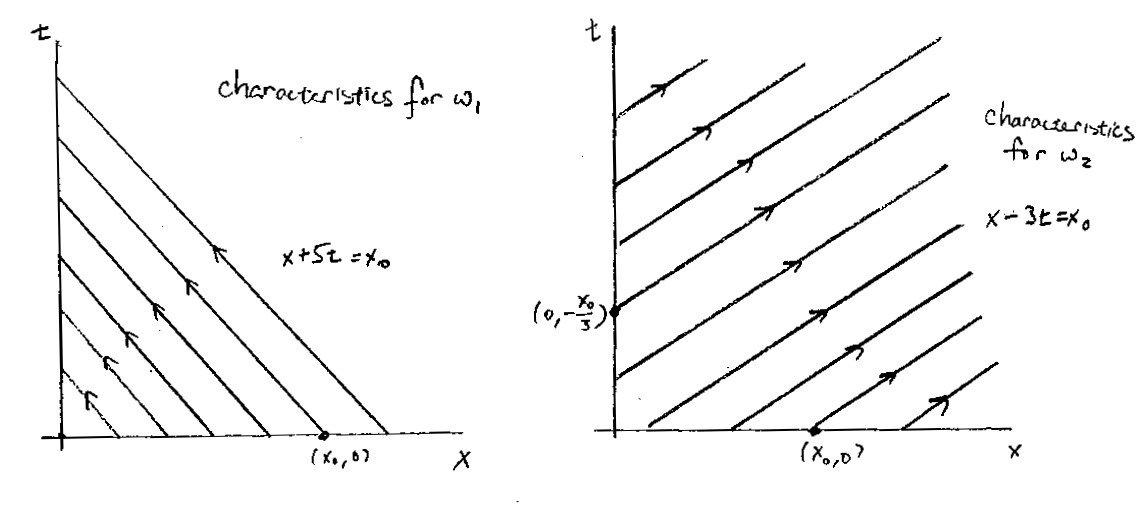
\includegraphics[scale=0.9]{./_Figures/F10Q2b.jpg}
\end{center}
Since $w_{1}$ is constant on characteristics,
\ba
w_{1}(x, t) = \frac{1}{2}f(x_0) + \frac{1}{2}g(x_0) = \frac{1}{2}f(x + 5t) + \frac{1}{2}g(x + 5t).
\ea
Then $w_{1}(0, t) = \frac{1}{2}f(5t) + \frac{1}{2}g(5t)$. As $cw_{1}(0, t) + dw_{2}(0, t) = 0$,
$$w_{2}(0, t) = -\frac{c}{2d}(f(5t) + g(5t)).$$
Since $w_{2}(x, 0) = \frac{1}{2}(f(x) - g(x))$,
\ba
w_{2}(x, t) &=
\begin{cases}
\frac{1}{2}(f(x - 3t) - g(x - 3t)) & \text{ if } x - 3t > 0\\
-\frac{c}{2d}(f(-\frac{5}{3}(x - 3t)) + g(-\frac{5}{3}(x - 3t))) & \text{ if } x - 3t < 0
\end{cases}\\
&=
\begin{cases}
\frac{1}{2}f(x - 3t) - \frac{1}{2}g(x - 3t) & \text{ if } x - 3t > 0\\
-\frac{c}{2d}f(5t - \frac{5}{3}x) - \frac{c}{2d}g(5t - \frac{5}{3}x) & \text{ if } x - 3t < 0.
\end{cases}
\ea
Thus the PDE is well posed as long as the boundary conditions for $w_{2}$ are compatible, that is,
we need $c$ and $d$ to be such that
$\lim_{t \rightarrow 0^{+}}w_{2}(0, t) = \lim_{x \rightarrow 0^{+}}w_{2}(x, 0)$.
That is,
$$-\frac{c}{2d}(f(0) + g(0)) = \frac{1}{2}(f(0) - g(0)).$$
Using that $c = a + b$, $d = a - b$, we have
$$\frac{a + b}{a - b} = \frac{g(0) - f(0)}{g(0) + f(0)}.$$
Rearranging yields
$af(0) = -bg(0)$.
Thus the set of $a, b$ which make the problem $\svt{u}{v}_{t} = \smat{1}{4}{4}{1}\svt{u}{v}_{x}$
with $u(x, 0) = f(x)$, $v(x, 0) = g(x)$, $au(0, t) + bv(0, t) = 0$ is precisely
the $a, b$ such that $af(0) = -bg(0)$.
\hq

\subsection*{Solution to Fall 2010, \#3}
\label{F10Q3}
\ssb{Solution to $(a)$}
The equilibria are $(0, 0)$, $(0, a_2/c_2)$, $(a_1/b_1, 0)$ and the solution to the system
$a_{1} = b_{1}x + c_{1}y$, $a_{2} = b_{2}x + c_{2}y$. Thus
$\svt{x}{y} = \smat{b_1}{c_1}{b_2}{c_{2}}^{-1}\svt{a_1}{a_2}$. Since $b_1 c_2 - b_2 c_1 \neq 0$, then
$\smat{b_1}{c_1}{b_2}{c_2}$ is invertible and hence the last equilibrium point is
\ba
\vct{x}{y} = \pmat{b_1}{c_1}{b_2}{c_{2}}^{-1}\vct{a_1}{a_2} = \frac{1}{b_1 c_2 - b_2 c_1}\pmat{c_2}{-c_1}{-b_2}{b_1}\vct{a_1}{a_2} = \frac{1}{b_1 c_2 - b_2 c_1}\vct{a_1 c_2 - a_2 c_1}{-a_1 b_2 + a_2 b_1}.
\ea
\hq

\ssb{Solution to $(b)$}
The equilibrium point in the open quarter plane is $(x_0, y_0)$ where
\ba
x_{0} = \frac{a_{1}c_{2} - a_{2}c_{1}}{b_{1}c_{2} - b_{2}c_{1}}, \quad y_{0} = \frac{a_{2}b_{1} - a_{1}b_{2}}{b_{1}c_{2} - b_{2}c_{1}}.
\ea
We will show that this point is a saddle. The Jacobian evaluated at $(x_{0}, y_{0})$ is
\ba
J(x_{0}, y_{0}) = \pmat{a_{1} - 2b_{1}x_{0} - c_{1}y_{0}}{-c_{1}x_{0}}{-b_{2}y_{0}}{a_{2} - b_{2}x_{0} - 2c_{2}y_{0}} = \pmat{-b_{1}x_{0}}{-c_{1}x_{0}}{-b_{2}y_{0}}{-c_{2}y_{0}}
\ea
where the last equality is because $a_{1} = b_{1}x_{0} + c_{1}y_{0}$ and $a_{2} = b_{2}x_{0} + c_{2}y_{0}$.
The eigenvalues of this matrix satisfy
\begin{align}\label{f103beq1}
\ld^2 + (c_{2}y_{0} + b_{1}x_{0})\ld + (b_{1}c_{2} - b_{2}c_{1})x_{0}y_{0} = 0.
\end{align}
Thus to prove the roots of \eqref{f103beq1} are distinct and real, it suffices to show that
$$(c_{2}y_{0} + b_{1}x_{0})^{2} - 4(b_{1}c_{2} - b_{2}c_{1})x_{0}y_{0} > 0.$$
We have
\ba
(c_{2}y_{0} + b_{1}x_{0})^2 - 4(b_{1}c_{2} - b_{2}c_{1})x_{0}y_{0} &= (c_{2}y_{0})^2 + (b_{1}x_{0})^2 - 2b_{1}c_{2}x_{0}y_{0} + 4b_{2}c_{1}x_{0}y_{0}\\
& = (c_{2}y_{0})^2 + (b_{1}x_{0})^2 + 2(b_{2}c_{1} - b_{1}c_{2})x_{0}y_{0} + 2b_{2}c_{!}x_{0}y_{0} > 0
\ea
since $b_{2}c_{1} - b_{1}c_{2} > 0$ and $b_{2}c_{1}x_{0} y_{0} > 0$. Thus $(x_{0}, y_{0})$ is a saddle.
\hq

\ssb{Solution to $(c)$}
%
%
%
% PICTURE
%
%
%
%

\subsection*{Solution to Fall 2010, \#4}
\label{F10Q4}

We use method of characteristics. Define $F(x,t,z,p,q) = q + zp + x = 0$, where $z := u$, $p := u_x$, and $q := u_t$. Then, we have
\begin{equation}
\label{f1041} \dot{t}(s) = 1, \quad t(0) = 0
\end{equation}
\begin{equation}
\label{f1042} \dot{x}(s) = z(s), \quad x(0) = x_0
\end{equation}
\begin{equation}
\label{f1043} \dot{z}(s) = -x(s), \quad z(0) = f(x_0)
\end{equation}
Solving \eqref{f1041} yields $t(s) = s$. Then combining \eqref{f1042} and \eqref{f1043} yields
\begin{equation}
\label{f1044}
\ddot{x}(s) + x(s) = 0, \quad x(0) = x_0, \,\,\, \dot{x}(0) = f(x_0)
\end{equation}
Solving \eqref{f1044} yields $x(s) = x_0 \cos(s) + f(x_0) \sin(s)$, and then plugging this back into \eqref{f1043} yields $z(s) = -x_0 \sin(s) + f(x_0) \cos(s)$. Thus, we have
$$ u(x,t) = -x_0 \sin(t) + f(x_0) \cos(t), \quad \text{where $x_0$ satisfies} \,\,\, x = x_0 \cos(t) + f(x_0) \sin(t) $$
If $f'(x) \geq 0$ for all $x$, we claim that the characteristics don't cross for $t \in (0,\pi/2)$. Indeed, if characteristics do cross, then, for $x_0 \neq x_1$,
$$ x_0 \cos(t) + f(x_0) \sin(t) = x_1 \cos(t) + f(x_1) \sin(t) $$
implies
$$ -\frac{\cos(t)}{\sin(t)} = \frac{f(x_1)-f(x_0)}{x_1 - x_0} \geq 0 $$
But $-\frac{\cos(t)}{\sin(t)} < 0$ for $t \in (0,\pi/2)$, which is a contradiction. Therefore, the solution will exist for $t \in [0,\pi/2)$. \hfill \qed


\subsection*{Solution to Fall 2010, \#5}
\label{F10Q5}
Note that as $\phi$ is smooth and 1-1, $u = 0$ on $\pr D$ if and only if $\wh{u} = 0$ on $\pr D$.
Let $v$ be smooth and of compact support. Then
\ba
\int_{D}-\sum_{i = 1}^{2}\pr_{x_{i}}(\beta(x)u_{x_{i}})v\, dx = \int_{D}fv\, dx.
\ea
We have
\ba
\int_{D}f(x)v(x)\,dx = \int_{\wh{D}}f(\phi^{-1}(y))v(\phi^{-1}(y))\wh{h}(y)\, dy = \int_{\wh{D}}\wh{f}\wh{v}\wh{h}\, dy
\ea
and
\ba
\int_{D}-\sum_{i =1}^{2}\pr_{x_i}(\beta(x)u_{x_i})v\, dx &= \int_{D}\sum_{i = 1}^{2}\beta(x)u_{x_i}v_{x_i}\, dx\\
& = \int_{\wh{D}}\sum_{i = 1}^{2}\beta(\phi^{-1}(y))u_{x_i}(\phi^{-1}(y))v_{x_{i}}(\phi^{-1}(y))\wh{h}(y)\, dy\\
& = \int_{\wh{D}}\wh{\beta}(y)\wh{h}(y)\sum_{i = 1}^{2}u_{x_i}(\phi^{-1}(y))v_{x_i}(\phi^{-1}(y))\, dy.
\ea
We have $y = \phi(x) = \svt{\phi_{1}(x)}{\phi_{2}(x)}$ and $\frac{\pr u}{\pr x_i} = \frac{\pr u}{\pr y_1}\frac{\pr y_1}{\pr x_i} + \frac{\pr u}{\pr y_2}\frac{\pr y_2}{\pr x_i}$.
Thus
\ba
u_{x_{i}}(\phi^{-1}(y)) = u_{y_i}(\phi^{-1}(y))(\phi_{1})_{x_i}(\phi^{-1}(y)) + u_{y_2}(\phi^{-1}(y))(\phi_2)_{x_i}(\phi^{-1}(y))
\ea
and we will write the right hand side as $\wh{u}_{y_1}\cdot (\phi_1)_{x_i} + \wh{u}_{y_2}\cdot (\phi_2)(x_i)$.
Thus
\ba
&\int_{\wh{D}}\wh{\beta}(y)\wh{h}(y)\sum_{i = 1}^{2}u_{x_i}(\phi^{-1}(y))v_{x_i}(\phi^{-1}(y))\, dy\\
& = \int_{\wh{D}}\wh{\beta}\wh{h}\sum_{i = 1}^{2}(\wh{u}_{y_1}(\phi_1)_{x_i} + \wh{u}_{y_2}(\phi_2)_{x_i})(\wh{v}_{y_1}(\phi_1)_{x_i} + \wh{v}_{y_2}(\phi_2)_{x_i})\, dy\\
& = \int_{\wh{D}}\wh{\beta}(y)\wh{h}(y) \sum_{i = 1}^{2}\bigg(\wh{u}_{y_{1}}(y)[(\phi_{1})_{x_{i}}(\phi^{-1}(y))]^{2} + \wh{u}_{y_{2}}(y)[(\phi_{1})_{x_{i}}(\phi^{-1}(y))][(\phi_{2})_{x_{i}}(\phi^{-1}(y))]\bigg)\wh{v}_{y_{1}}(y)\\
&\,\,\,\,\, + \bigg(\wh{u}_{y_{1}}(y)[(\phi_{1})_{x_{i}}(\phi^{-1}(y))][(\phi_{2})_{x_{i}}(\phi^{-1}(y))] + \wh{u}_{y_{2}}(y)[(\phi_{2})_{x_{i}}(\phi^{-1}(y))]^{2}\bigg)\wh{v}_{y_{2}}(y)\\
&= \int_{\wh{D}}\wh{\beta}(y)\wh{h}(y)\sum_{i = 1}^{2}M_{i}\vct{\wh{y_{1}}(y)}{\wh{u}_{y_{2}}(y)}\cdot \del \wh{v}\, dy
\ea
where
\ba
M_{i} = \pmat{[(\phi_1)_{x_i}(\phi^{-1}(y))]^{2}}{[(\phi_{1})_{x_i}(\phi^{-1}(y))][(\phi_2)_{x_i}(\phi^{-1}(y))]}{[(\phi_{1})_{x_i}(\phi^{-1}(y))][(\phi_2)_{x_i}(\phi^{-1}(y))]}{[(\phi_2)_{x_i}(\phi^{-1}(y))]^{2}}.
\ea
Since
\ba
\int_{\wh{D}}\vec{u}\cdot \del v\, dx = -\int_{\wh{D}}\del \cdot \vec{u} v\, dx,
\ea
we have
\ba
\int_{\wh{D}}\wh{\beta}(y)\wh{h}(y)\sum_{i = 1}^{2}M_{i}\vct{\wh{y_{1}}(y)}{\wh{u}_{y_{2}}(y)}\cdot \del \wh{v}\, dy = -\int_{\wh{D}}\del \cdot \bigg(\wh{h}(y)(\sum_{i = 1}^{2}\wh{\beta}(y)M_i)\vct{\wh{u}_{y_1}(y)}{\wh{u}_{y_{2}}(y)}\bigg)\wh{v}(y)\, dy.
\ea
Let $N := \wh{\beta}(y)(M_1 + M_2)$. Then
\ba
N\vct{\wh{u}_{y_{1}}}{\wh{u}_{y_{2}}} = \vct{N_{11}\wh{u}_{y_{1}} + N_{12}\wh{u}_{y_2}}{N_{21}\wh{u}_{y_{1}} + N_{22}\wh{u}_{y_{2}}}.
\ea
Thus
\ba
\del \cdot (\wh{h}(y)N\vct{\wh{u}_{y_{1}}}{\wh{u}_{y_{2}}}) = \sum_{j = 1}^{2}\frac{\pr}{\pr y_{j}}(\wh{h}(y)\sum_{k = 1}^{2}N_{jk}(y)\wh{u}_{y_k}(y)).
\ea
Therefore we have
\ba
-\int_{\wh{D}}\sum_{i = 1}^{2}\frac{\pr}{\pr y_{i}}(\wh{h}(y)\sum_{j =1}^{2}N_{ij}(y)\frac{\pr\wh{u}}{\pr y_j}(y))\wh{v}(y)\, dy = \int_{\wh{D}}\wh{f}(y)\wh{h}(y)\wh{v}(y)\, dy
\ea
which proves the desired result.
\hq



\subsection*{Solution to Fall 2010, \#6}
\label{F10Q6}

\subsubsection*{Solution to $6a$}

Suppose $a > 1$, and define $V = \sq{u \in H^1(\Omega) \, : \, \frac{\partial u}{\partial n} = 0}$. Because of the homogeneous Neumann boundary condition, it's easy to verify that the (positive) Laplacian operator is a symmetric elliptic operator. (Note: symmetric in this sense means that the associated bilinear form satisfies $B[u,v] = B[v,u]$ for all $u,v \in V$.) This implies that there exists an orthogonal basis of eigenfunctions $\{\varphi_n\}_{n \in \N}$ associated with the eigenvalues $\{\lambda_n\}_{n \in \N}$. Note that 0 is an eigenvalue since all constant functions are associated eigenfunctions. Without loss of generality, let $\lambda_1 = 0$ and $\varphi_1(x) = 1/|\Omega^a|^{1/2}$, where $|\Omega^a|$ two-dimensional area of $\Omega^a$. From this, we suppose our solution has the form
$$ u(x) = \sum_{n=1}^{\infty} \alpha_n \varphi_n(x) $$
for some sequence $\{\alpha_n\}_{n \in \N}$. Because $\{\varphi_n\}_{n \in \N}$ is an orthogonal basis of eigenfunctions, we have
$$ f(x) = \sum_{n=1}^{\infty} f_n \varphi_n(x), \quad \text{where} \,\,\, f_n = \frac{\int_{\Omega^a} f(x) \varphi_n(x) \, dx}{\int_{\Omega^a} \varphi_n^2(x) \, dx} $$
Then, for $n \geq 2$,
$$ \Delta u = f \quad \implies \quad \lambda_n \alpha_n = f_n \quad \implies \quad \alpha_n = \frac{f_n}{\lambda_n} $$
Observe
$$ \Delta \varphi_1 = 0, \quad \text{and} \quad f_1 = \frac{1}{|\Omega^a|^{1/2}} \int_{\Omega^a} f(x) \, dx = 0 $$
so we may choose $\alpha_1=0$. Hence,
$$ u(x) = \sum_{n=2}^{\infty} \frac{f_n}{\lambda_n} \varphi_n(x) $$
Therefore, for $a>1$, a solution exists.

Now, suppose $0<a<1$. This implies that $\Omega^a$ is now disconnected. Suppose there exists a solution $u$ to the Neumann problem in this case. Then,
\begin{align*}
\int_{\Omega_+^a} \Delta u \, dx = \int_{\Omega_+^a} f \, dx \quad \implies \quad 0 = 1	
\end{align*}
which is a contradiction. Integration by parts was applied to the integral on the left, and the integral over the boundary vanishes because of the homogeneous Neumann boundary condition on $u$. Hence, no solution exists when $0<a<1$.

\subsubsection*{Solution to $6b$}

Fix $a>1$, and let $L^a = \partial \Omega_+^a \cap \Omega_-^a$. Then,
$$ 1 = \int_{\Omega_+^a} f \, dx = \int_{\Omega_+^a} \Delta u \, dx = \int_{\partial \Omega_+^a} \frac{\partial u}{\partial n} \, dx = \int_{L^a} \frac{\partial u}{\partial n} \, dx $$
Hence,
$$ 1 \leq |L^a| \sup_{L^a} \left| \frac{\partial u}{\partial n} \right| \leq |L^a| \sup_{\Omega^a} |\nabla u| $$
where $|L^a|$ is the length of $L^a$. We obtain the second inequality because $L^a \subset \Omega^a$. Then,
$$ \frac{1}{|L^a|} \leq \sup_{\Omega^a} |\nabla u| $$
Decreasing $a$ to $1$ means $|L^a| \to 0$, which yields
$$\sup_{\Omega^a} |\nabla u| \to \infty$$ \hfill \qed


\subsection*{Solution to Fall 2010, \#7}
\label{F10Q7}

Define $y(x,t) := u(x,t) - w(x)$, and observe
\begin{equation}
\label{f107heat}
	y_t - \Delta y = u_t - \Delta u + \Delta w = 0
\end{equation}
with $y(x,t) = 0$ on $\partial D$ and $y(x,0) = -w(x)$. Now, suppose $y(x,t) = F(x)G(t)$ for some functions $F$ and $G$. Plugging this into \eqref{f107heat} yields
$$ F(x) G'(t) - \Delta F(x) G(t) = 0 \quad \implies \quad \frac{G'(t)}{G(t)} = \frac{ \Delta F(x)}{F(x)} = -\mu $$
where $\mu$ is an arbitrary constant. This provides us with an ODE for $x$:
\begin{equation}
\label{f107eq1}
-\Delta F(x) = \mu F(x), \quad F = 0 \,\, \text{on} \,\, \partial D
\end{equation}	
We also have an ODE for $t$, but we aren't going to worry about it until after we solve \eqref{f107eq1}. Note that \eqref{f107eq1} is an eigenvalue problem for the (negative) Laplacian operator with homogeneous boundary conditions. It's straightforward to see that the operator is a symmetric elliptic operator, implying that there exists an orthogonal basis of eigenfunctions $\{\varphi_n\}_{n \in \N}$ with associated eigenvalues $\{ \lambda_n \}_{n \in \N}$. It's also easy to verify that $\lambda_n > 0$ for all $n \in \N$. From this, for each $n \in \N$, we obtain an ODE for $t$:
$$ G_n'(t) = -\lambda_n G_n(t) $$
(Note, by the superposition principle, we are now supposing that our solution takes the form $y(x,t) = \sum_{n=1}^{\infty} G_n(t) \varphi_n(x)$.) To obtain the initial conditions for this family of ODEs, we need to first represent $y(x,0) = -w(x)$ in terms of the eigenfunctions:
$$ -w(x) = \sum_{n=1}^{\infty} \alpha_n \varphi_n(x), \quad \text{where} \,\,\, \alpha_n = \frac{-\int_D w(x) \varphi_n(x) \, dx}{\int_D \varphi_n^2(x) \, dx} $$
Hence, for each $n \in \N$, we have
$$ G'_n(t) = -\lambda_n G_n(t), \quad G_n(0) = \alpha_n \quad \implies \quad G_n(t) = \alpha_n e^{-\lambda_n t} $$
Putting everything together yields
$$ y(x,t) = \sum_{n=1}^{\infty} \alpha_n e^{-\lambda_n t} \varphi_n(x) $$
Therefore,
$$ u(x,t) = w(x) + \sum_{n=1}^{\infty} \alpha_n e^{-\lambda_n t} \varphi_n(x) $$
Furthermore, there is no leading term in the asymptotic expansion of $u(x,t) - w(x)$ as $t \to \infty$ because $\lambda_n > 0$ for all $n \in \N$ --- all of the terms vanish in the limit. \hfill \qed



\subsection*{Solution to Fall 2010, \#8}
\label{F10Q8}

Let $E(t) := \frac{1}{2} \int_D u_t^2 + |\nabla u|^2 \, dx$. Then, differentiating with respect to $t$ and applying integration by parts yields
$$ \dot{E}(t) = \int_D u_t u_{tt} + \nabla u \cdot \nabla u_t \, dx = \int_D u_t u_{tt} - \Delta u u_t \, dx $$
Because $u$ vanishes on the boundary, the boundary integral that arises from integration by parts vanishes. Thus,
$$ \dot{E}(t) = - \int_D (a(x,t)u_t)^2 \, dx \leq 0 $$
Since $E(0) = \frac{1}{2} \int_D g(x)^2 + |\nabla f(x)|^2 \, dx < \infty $, we have
$$ 0 \leq E(t) \leq E(0) $$
for all $t$. Since $u=0$ on $\partial D$, by Poincare's inequality,
$$ \int_D u^2 \, dx \leq C_D \int_D |\nabla u|^2 \, dx \leq 2C_D E(t) \leq 2C_D E(0) $$
where $C_D$ is a constant that only depends on $D$. Therefore, $\int_D u^2 \, dx$ is bounded. \hfill \qed


\section{Spring 2010}\label{s10}
\subsection*{Solution to Spring 2010, \#1}\label{s101}
There seems to be a typo in the problem, we will show that all eigenvalues must
be less than $-1$. (It is not uncommon to see people call $\ld$ the
eigenvalue for the Sturm-Liouville problem $Lu = -\ld u$. But strictly speaking
from a linear algebra point of view, $-\ld$ is the eigenvalue for $L$ not $+\ld$.)

Let $y$ be an eigenfunction. Then $y$ is not identically zero. We have
$\ips{y'' - y, y} = \ips{-\ld x^{2}y', y}$, that is,
$$\int_{0}^{1}y''y - y^{2}\, dx = -\ld \int_{0}^{1}x^{2}y'y\, dx.$$
Integration by parts yields that
$$\int_{0}^{1}y''y\, dx = -\int_{0}^{1}y'^{2}\, dx$$
and
$$\int_{0}^{1}x^{2}y'y\, dx = \int_{0}^{1}x^{2}(\frac{1}{2}y^{2})'\, dx = -\int_{0}^{1}xy^{2}\, dx.$$
Therefore
\begin{align*}
-\ld = \frac{\int_{0}^{1}y'^{2} + y^{2}\, dx}{\int_{0}^{1}xy^{2}\, dx} \geq \frac{\int_{0}^{1}y'^{2} + y^{2}\, dx}{\int_{0}^{1}y^{2}\, dx} = 1 + \frac{\int_{0}^{1}y'^{2}\, dx}{\int_{0}^{1}y^{2}\, dx} \geq 1.
\end{align*}
Thus $\ld \leq -1$.
\hfill\qed

\subsection*{Solution to Spring 2010, \#2}\label{s102}
We present two solutions to this problem, one emphasising the important ``$L^{p}$ trick" (see the appendix for a more detailed discussion),
and another emphasising a maximum principle approach. Note that since $g$ is compactly supported in $\Om$, we actually have
$u(x, t) = 0$ on $\pr \Om \times [0, \infty)$.

\begin{rem}
The $L^{p}$ trick may seem a bit more tedious than a maximum principle solution, however it is much more robust approach, especially when a
maximum principle approach is not so obvious or hard to prove, see for example, Spring 2008 Question 7 or Spring 2014 Question 2.
\end{rem}

\subsubsection*{``$L^{p}$ trick" Solution}
As $\Om$ is a bounded domain with smooth boundary, $\Om$ has finite measure. Therefore
\begin{align}\label{s102eq1}
\lim_{p \rightarrow \infty}\|u(x, t)\|_{L^{p}_{x}(\Om)} = \|u(x, t)\|_{L^{\infty}_{x}(\Om)}.
\end{align}
Thus to control the $L^{\infty}$ norm of $u$, it suffices to control each $L^{p}$ norm. Let $\psi(x) := |x|^{p}$ for $p > 2$.
Note that $\psi$ is $C^{2}$ for $p > 2$. Let $$E(t) := \int_{\Om}\psi(u)\, dx = \int_{\Om}|u|^{p}\, dx.$$
Then
\begin{align*}
\dot{E}(t) &= \int_{\Om}\psi'(u)u_{t}\, dx = \int_{\Om}\psi'(u)(\Delta u - u)\, dx = -\int_{\Om}\nabla (\psi'(u)) \cdot \nabla u + \psi'(u)u\, dx\\
&= -\int_{\Om}\psi''(u)\sum_{i = 1}^{n}u_{x_{i}}^{2} + \psi'(u)u\, dx \leq -\int_{\Om}\psi'(u)u\, dx = -p\int_{\Om}\psi(u)\, dx = -pE(t).
\end{align*}
where the last equality is because $x(\frac{d}{dx}|x|^{p}) = p|x|^{p}$. Therefore
by Gronwall's inequality, $E(t) \leq e^{-pt}E(0)$. Taking $1/p$-th powers of both sides gives that
$$\|u(x, t)\|_{L^{p}_{x}(\Om)} = \bigg(\int_{\Om}|u(x, t)|^{p}\, dx\bigg)^{1/p} \leq e^{-t}\bigg(\int_{\Om}|u(x, 0)|^{p}\, dx\bigg)^{1/p} = e^{-t}\|g\|_{L^{p}(\Om)}.$$
Using \eqref{s102eq1} yields that
$$\|u(x, t)\|_{L^{\infty}_{x}(\Om)} \leq e^{-t}\|g\|_{L^{\infty}(\Om)}.$$
Since $u$ is a $C^{2}$ solution the $L^{\infty}$ norm is just the sup norm and hence it follows that
$|u(x, t)| \leq e^{-t}\|g\|_{L^{\infty}}$ for all $t > 0$.
\hfill\qed

\subsubsection*{Maximum Principle Solution}
Let $v := ue^{t}$. Then $v_{t} = u_{t}e^{t} + ue^{t} = (u_{t} + u)e^{t}$
and $\Delta v = e^{t}\Delta u$. Therefore
$v_{t} - \Delta v = (u_{t} + u)e^{t} - e^{t}\Delta u = 0$. Thus we have
\begin{align*}
\begin{cases}
v_{t} - \Delta v = 0 & \text{ in } \Delta \times (0, \infty)\\
v(x, 0) = g(x) & \text{ in } \Om\\
v(x, t) = 0 & \text{ in } \pr\Om \times (0, \infty).
\end{cases}
\end{align*}
Therefore by the maximum principle, $v(x, t) \leq \|g\|_{L^{\infty}}$. Replacing $v$ with $-v$ shows that
$|v(x, t)| \leq \|g\|_{L^{\infty}}$ and hence $|u(x, t)| \leq \|g\|_{L^{\infty}}e^{-t}$ for all $t > 0$.
\hfill\qed

\subsection*{Solution to Spring 2010, \#3}\label{s103}
We present two solutions to this problem.

\subsubsection*{Maximum Principle Solution}
Let $U, v $ be two $C^{2}$ solutions and $w = u - v$. Then
\begin{align*}
\begin{cases}
-\Delta w + a(x)w = 0 & \text{ in } \Om\\
\pr w/\pr \nu = 0 & \text{ on } \pr\Om.
\end{cases}
\end{align*}
If there exists $x_{0} \in \pr \Om$ such that
$w(x) < w(x_{0})$ for all $x \in \Om$< then by Hopf's Lemma,
$\frac{\pr w}{\pr \nu}(x_{0}) > 0$. This is a contradiction
and hence no such $x_{0}$ exists.

Since $w$ is continuous on the compact set $\ov{\Om}$,
there exists $x_{0} \in \ov{\Om}$ such that
$w(x) \leq w(x_{0})$ for all $x \in \ov{\Om}$.

Suppose
$x_{0} \in \pr\Om$. Then $w(x) \leq w(x_{0})$ for all $x \in \Om$.
Then by the argument in the previous paragraph, there exists
an $x' \in \Om$ such that $w(x') = w(x_{0})$. Therefore
$w$ attains a maximum in the interior of $\ov{\Om}$ and hence
by the Maximum Principle, $w$ is a constant. Since
$a(x) > 0$ and $0 = -\Delta w + a(x)w = a(x) w$ (as $w$ is constant),
it follows that $w \equiv 0$ in this case.

Next suppose $x_{0} \in \Om$. Then again $w$ attains a maximum
in the interior of $\ov{\Om}$ and hence $w \equiv 0$ by the same
argument as above in the previous paragraph.

Thus $u \equiv v$ which proves uniqueness.
\hfill\qed

\subsubsection*{``Energy" Solution}
Let $w$ be as in the previous solution.
Suppose $w > 0$ on some open subset $U \subset \Om$. Then
\begin{align*}
0 = \int_{\Om}-\Delta w + a(x)w\, dx = \int_{\pr \Om}-\frac{\pr w}{\pr \nu}\, d\sigma + \int_{\Om}a(x)w\, dx \geq \int_{U}a(x)w\, dx > 0
\end{align*}
a contradiction. Therefore $w \leq 0$ on $\Om$. However, a similar argument
shows that we cannot have $w < 0$ on some $V \subset \Om$ and hence $w \geq 0$ on $\Om$. Therefore
$w \equiv 0$ on $\Om$.
\hfill\qed

\subsection*{Solution to Spring 2010, \#4}\label{s104}
\subsubsection*{Solution to $4a$}
If $u$ was compactly supported, then we would choose
$$E(t) := \frac{1}{2}\int_{\R}u_{t}^{2} + u_{x}^{2} + u^{2}\, dx.$$
Then
$$\dot{E}(t) = \int_{\R}u_{t}u_{tt} + u_{x}u_{xt} + uu_{t}\, dx = \int_{\R}u_{t}u_{tt} - u_{xx}u_{t} + uu_{t}\, dx = \int_{\R}u_{t}(-u) + uu_{t}\, dx = 0.$$
In the next part, we will show that $u$ is indeed compactly supported.
\hfill\qed

\subsubsection*{Solution to $4b$}
We will prove the statement in $d$-dimensions, so we are working with the equation $u_{tt} - \Delta u = -u$ in $\R^{d} \times (0, \infty)$
and $u(x, 0) = g(x)$, $u_{t}(x, 0) = h(x)$ with $g, h \in C_{c}(\R^{d})$. Let $u \equiv u_{t} \equiv 0$ in $B(x_{0}, t_{0})$ (ball of radius $t_{0}$ centered at $x_{0}$), then we claim
$u \equiv 0$ in the cone $C = \{(x, t): 0 \leq t \leq t_{0}, |x - x_{0}| \leq t_{0} - t\}$.

The proof will be similar to the finite speed of propagation proof for the wave equation.
For $0 \leq t \leq t_{0}$, let
$$E(t) := \frac{1}{2}\int_{B(x_{0}, t_{0} - t)}u_{t}^{2} + |\nabla u|^{2} + u^{2}\, dx.$$
Then
\begin{align*}
\dot{E}(t) &= \int_{B(x_{0}, t_{0} - t)}u_{t}u_{tt} + \nabla u \cdot \nabla u_{t} + uu_{t}\, dx - \frac{1}{2}\int_{\pr B(x_{0}, t_{0} - t)}u_{t}^{2} + |\nabla u|^{2} + u^{2}\, d\sigma\\
&= \int_{B(x_{0}, t_{0} - t)}u_{t}u_{tt} - \Delta u u_{t} + u u_{t}\, dx\\
&\hspace{2in}+ \int_{\pr B(x_{0}, t_{0} - t)}\frac{\pr u}{\pr \nu}u_{t}\, d\sigma - \frac{1}{2}\int_{\pr B(x_{0}, t_{0} - t)}u_{t}^{2} + |\nabla u|^{2} + u^{2}\, d\sigma\\
&\leq \int_{B(x_{0}, t_{0} - t)}u_{t}(u_{tt} - \Delta u + u)\, dx + \int_{\pr B(x_{0}, t_{0} - t)}\frac{\pr u}{\pr \nu}u_{t} - \frac{1}{2}u_{t}^{2} - \frac{1}{2}|\nabla u|^{2}\, d\sigma.
\end{align*}
Since $u_{tt} - \Delta u + u = 0$ and
\begin{align*}
\frac{\pr u}{\pr \nu}u_{t} \leq \abb{\frac{\pr u}{\pr \nu}u_{t}} \leq \frac{1}{2}u_{t}^{2} + \frac{1}{2}|\nabla u|^{2},
\end{align*}
it follows that $\dot{E}(t) \leq 0$ for $0 \leq t \leq t_{0}$. Therefore $E(t) \leq E(0) = 0$ for all $0 \leq t \leq t_{0}$. Thus
$u \equiv 0$ in the cone $C$.

Since $g$ and $h$ are both compactly supported, let $M$ be such that $g(x) = 0$ and $h(x) = 0$
for $|x| > M$. Fix a time $T > 0$. We show that $u(\cdot, T)$ is compactly supported.
For $|x_{0}| > M + 2T$, then $u \equiv u_{t} \equiv 0$ in $B(x_{0}, T)$. By the computation
in the previous paragraph, it follows that $u \equiv 0$ in $\{(x, t) : 0 \leq t \leq T, |x - x_{0}| \leq T - t\}$. In particular, $(x_{0}, T)$ is in this set and hence $u(x_{0}, T) = 0$.
Therefore since $x_{0}$ was an arbitrary point with length $> M + 2T$, it follows
that $u(x, T) = 0$ for all $|x| > M + 2T$. Therefore $u$ is compactly supported.
\hfill\qed

\subsection*{Solution to Spring 2010, \#5}\label{s105}
Let $v : \R \times [0,\infty)$ be smooth with compact support. Then, by integration by parts,
\begin{align}
\nonumber 0 &= \int_0^{\infty} \int_{-\infty}^{\infty} [(g(u))_t + (h(u))_x] v \, dx dt \\
\nonumber &= -\int_0^{\infty} \int_{-\infty}^{\infty} g(u)v_t + h(u)v_x \, dx dt + \int_{-\infty}^{\infty} g(u)v \Bigr\rvert_{0}^{\infty} \, dx \\
\label{s10intsol} &= \int_0^{\infty} \int_{-\infty}^{\infty} g(u)v_t + h(u)v_x \, dx dt + \int_{-\infty}^{\infty} g(u(x,0))v(0) \, dx
\end{align}
Because $v$ has compact support many of the boundary terms vanish. \eqref{s10intsol} is the integral solution.

\vspace{0.4cm}

Suppose $C$ is a smooth curve in $\R \times (0,\infty)$ such that $u$ is not continuous on $C$, but is smooth on either side. Let $V \subset \R \times (0,\infty)$ be open such that $V \cap C \neq \emptyset$. Let $V_l$ denote the part of $V$ to the left of $C$ and $V_r$ denote the part of $V$ to the right of $C$. Let $v$ be a smooth test function with compact support in $V$. Then, using \eqref{s10intsol},
\begin{align}
	\nonumber 0 &= \int_0^{\infty} \int_{-\infty}^{\infty} g(u)v_t + h(u)v_x \, dx dt + \int_{-\infty}^{\infty} g(u(x,0))v(0) \, dx \\
	\label{s10twoint} &= \iint_{V_l} g(u)v_t + h(u)v_x \, dx dt + \iint_{V_r} g(u)v_t + h(u)v_x \, dx dt
\end{align}
Note because $v$ has compact support in $V$, $v(0)=0$, so the second term in \eqref{s10intsol} vanishes. Now, using integration by parts, we compute
\begin{align*}
 \iint_{V_l} g(u) v_t + h(u) v_x \, dx dt &= -\iint_{V_l} [(g(u))_t + (h(u))_x] v \, dx dt + \int_C [g(u_-) \nu^2 + h(u_-) \nu_1] v \, dl \\
 &= \int_C [g(u_-) \nu^2 + h(u_-) \nu_1] v \, dl
\end{align*}
Recall that $v$ has compact support in $V$, so the integral along $\d V_l \backslash C$ that arises from integration by parts vanishes. The notation $u_-$ denotes taking a limit from left to right toward $C$. Finally $\nu = (\nu^1,\nu^2)$ is the unit normal to $C$ pointing from $V_l$ to $V_r$. By similar work,
$$ \iint_{V_r} g(u) v_t + h(u) v_x \, dx dt = - \int_C [g(u_+) \nu^2 + h(u_+) \nu_1] v \, dl $$
We get an extra negative sign here because $\nu$ is pointing in the opposite direction of what the normal vector should be. Thus, \eqref{s10twoint} becomes
\begin{align*}
0 &= \int_C [g(u_-) \nu^2 + h(u_-) \nu_1] v \, dl - \int_C [g(u_+) \nu^2 + h(u_+) \nu_1] v \, dl \\
&= \int_C [(g(u_-) - g(u_+))\nu^2 + (h(u_-)-h(u_+)) \nu_1]v \, dl
\end{align*}
Since this holds for all smooth test functions $v$ with compact support in $V$, we have
\begin{equation}
\label{s10RH}
	(g(u_-) - g(u_+))\nu^2 + (h(u_-)-h(u_+)) \nu_1 = 0
\end{equation}
along $C$. Suppose $C$ is parametrically represented as $\{(x,t) \, | \, x = s(t) \}$ for some smooth $s(\cdot) : [0,\infty) \to \R$. Then, because the tangential vector to $C$ at any $t$ is $(\dot s,1)$, the normal vector could be defined as $(1,-\dot s)$. Thus,
$$ \nu = (\nu^1,\nu^2) = \frac{1}{\sqrt{1+\dot s^2}} ( 1, -\dot s) $$
Therefore, \eqref{s10RH} becomes
$$ (g(u_-) - g(u_+))(-\dot s) + (h(u_-)-h(u_+)) = 0 \quad \implies \quad \dot s = \frac{h(u_-)-h(u_+)}{g(u_-) - g(u_+)} $$
which is the Rankine-Hugoniot condition along $C$. \hfill\qed

\subsection*{Solution to Spring 2010, \#6}\label{s106}
We use method of characteristics. We have
\begin{align*}
\begin{array}{ll}
 \dot{x} = 2p & x(0) = x_{0}\\
 \dot{y} = y & y(1) = 1\\
 \dot{p} = p & p(0) = \frac{1}{2}x_{0}\\
 \dot{q} = 0 & q(0) = 1\\
 \dot{z} = p^{2} + z & z(0) = \frac{1}{4}x_{0}^{2} + 1.
\end{array}
\end{align*}
Therefore we have $q(s) = 1$, $p(s) = \frac{1}{2}x_{0}e^{s}$, $x(s) = x_{0}e^{s}$, $y(s) = e^{s}$.
We have
$$\dot{z} = p^{2} + z = \frac{1}{4}x_{0}^{2}e^{2s} + z$$
and hence as $z(0) = \frac{1}{4}x_{0}^{2} + 1$,
$$z(s) = \frac{1}{4}x_{0}^{2} e^{2s} + e^{s} = \frac{1}{4}x_{0}^{2}\bigg(\frac{x(s)}{x_{0}}\bigg)^{2} + y(s) = \frac{1}{4}x(s)^{2} + y(s).$$
Therefore $u(x, y) = \frac{1}{4}x^{2} + y.$
\hfill\qed

\subsection*{Solution to Spring 2010, \#7}\label{s107}
We will write
$$E[u] := \frac{1}{2}\int_{0}^{x_{\Gamma}}\beta u'^{2}\, dx + \int_{x_{\Gamma}}^{1}\beta u'^{2}\, dx + \ov{u}b$$
where the derivative inside the integral are with respect ot $x$. For $f \in H^{1}$, with $f(0) = f(1) = [f] = 0$\footnote{We are choosing
$f$ so that $u + \vep f$ has the ``same properties" as $u$, so $(u + \vep f)(0) = (u + \vep f)(1) = 0$ and $[u + \vep f] = a$.}, we have
\begin{align*}
E'[u]f &= \lim_{\vep \rightarrow 0}\frac{1}{\vep}(E[u + \vep f] - E[u])\\
&= \int_{0}^{x_{\Gamma}}\beta u'f'\, dx + \int_{x_{\Gamma}}^{1}\beta u'f'\, dx + \ov{f}b = \int_{0}^{x_{\Gamma}}\beta u'f'\, dx + \int_{x_{\Gamma}}^{1}\beta u'f'\, dx + f(x_{\Gamma})b
\end{align*}
where the last equality is because $\ov{f} = f(x_{\Gamma})$ since $[f] = 0$.
Since $\frac{\pr}{\pr x}(\beta(x)u'(x)) = 0$ for $x \in (0, x_{\Gamma}) \cup (x_{\Gamma}, 1)$, $\beta u'$ is constant
in $(0, x_{\Gamma})$ and constant in $(x_{\Gamma}, 1)$. Let
\begin{align*}
\beta u' =
\begin{cases}
b_{0} & \text{ in } (0, x_{\Gamma})\\
b_{1} & \text{ in } (x_{\Gamma}, 1).
\end{cases}
\end{align*}
Then $b_{1} - b_{0} = b$ and hence
\begin{align*}
\int_{0}^{x_{\Gamma}}b_{0}f'\, dx &+ \int_{x_{\Gamma}}^{!}b_{1}f'\, dx + f(x_{\Gamma})(b_{1} - b_{0})\\
&= b_{0}(f(x_{\Gamma}) - f(0)) + b_{1}(f(1) - f(x_{\Gamma})) + f(x_{\Gamma})(b_{1} - b_{0}) = b_{1}f(1) - b_{0}f(0) = 0.
\end{align*}
Therefore $E'[u]f = 0$ for all such $f \in H^{1}$ with $f(0) = f(1) = [f] = 0$ and hence $E'[u] = 0$.

We also have
\begin{align*}
E''[u]f^{2} = \lim_{\vep \rightarrow 0}\frac{1}{\vep}(E'[u + \vep f]f - E'[u]f) = \int_{0}^{x_{\Gamma}}\beta f'^{2} + \int_{x_{\Gamma}}^{1}\beta f'^{2}\, dx > 0.
\end{align*}
Therefore $E''[u] > 0$. Thus $u$ is a minimum for $E[\, \cdot \,]$. That is, for all $v$ with $v \in H^{!}$
$v(0) = v(1) = 0$, $[v] = a$, we have $E[u] \leq E[v]$.
\hfill\qed

\subsection*{Solution to Spring 2010, \#8}\label{s108}
This is your basic ``Duhamel's principle" question. By the superposition principle, we can obtain the solution by solving
\begin{equation}
	\label{s101_8}
	\begin{array}{c}
	w_t + aw_x = f(x,t), \quad x \in \R, \,\, t > 0 \\
	w(x,0) = 0
	\end{array}
\end{equation}
and
\begin{equation}
	\label{s102_8}
	\begin{array}{c}
	v_t + av_x = 0, \quad x \in \R, \,\, t>0 \\
	v(x,0) = \phi(x)
	\end{array}
\end{equation}
and adding the results. The solution of \eqref{s102_8} is just $v(x,t) = \phi(x-at)$. To solve \eqref{s101_8}, we use Duhamel's principle, and instead, we solve
\begin{equation}
	\label{s103_8}
	\begin{array}{c}
	\tilde w_t(x,t;s) + a \tilde w_x(x,t;s) = 0, \quad x \in \R, \,\, t > s \\
	\tilde w(x,s;s) = f(x,s), \quad s>0
	\end{array}
\end{equation}
Then, we obtain $w$ by $w(x,t) = \int_0^t \tilde w(x,t;s) \, ds$. Thus, we have
$$ w(x,t) = \int_0^t f(x-a(t-s),s) \, ds $$
Therefore,
$$ u(x,t) = \phi(x-at) + \int_0^t f(x-a(t-s),s) \, ds $$ \hfill\qed


\section{Fall 2009}\label{f09}
\noindent The solution to Fall 2009, \#3 is omitted.

\sub{Solution to Fall 2009, \#1}\label{f091}
Note that $u(x)$ is harmonic in the open ball of radius $R$ not the closed ball of radius $R$, so we cannot immediately
apply Poisson's formula for a ball of radius $R$, rather we need to apply this formula to a ball of radius $R - \vep$.
See Winter 2005, \#3 for a similar solution.

We will assume $n \geq 3$.
Fix $x \in B_{R}(0)$. Let $\vep$ be such that $\vep \in (0, R - \abn{x})$. Then $x \in B_{R - \vep}(0)$ and by the Poisson formula for the ball,
\ba
u(x) = \frac{(R - \vep)^2 - \abn{x}^2}{n\alpha(n)(R - \vep)}\int_{\pr B(0, R - \vep)}\frac{u(y)}{\abn{x - y}^n}\, d\sigma(y).
\ea
Note that for $y \in \pr B(0, R - \vep)$, $R - \vep - \abn{x} \leq \abn{x - y} \leq R - \vep + \abn{x}$.
Thus
\ba
u(x) &\geq \frac{(R - \vep)^2 - \abn{x}^2}{n\alpha(n)(R - \vep)}\int_{\pr B(0, R - \vep)}\frac{u(y)}{(R - \vep - \abn{x})^n}\, d\sigma(y)\\
& = \frac{(R - \vep)^2 - \abn{x}^2}{n\alpha(n)(R - \vep)(R - \vep- \abn{x})^n}\int_{\pr B(0, R - \vep)}u(y)\, d\sigma(y)\\
& = \frac{(R - \vep)^2 - \abn{x}^2}{(R - \vep)(R - \vep - \abn{x})^n}(R - \vep)^{n - 1}u(0) \\
&= \frac{(R - \vep)^2 - \abn{x}^2}{(R - \vep - \abn{x})^n}(R -\vep)^{n - 2}u(0)
\ea
where the second equality we have used that $u$ is harmonic in the open ball of radius $R$ (and hence is harmonic in the closed ball of radius $R - \vep$).
Similarly,
\ba
u(x) = \frac{(R - \vep)^2 - \abn{x}^2}{n\alpha(n)(R - \vep)}\int_{\pr B(0, R - \vep)}\frac{u(y)}{\abn{x - y}^n}\, d\sigma(y) \leq \frac{(R - \vep)^2 - \abn{x}^2}{(R - \vep + \abn{x})^n}(R - \vep)^{n - 2}u(0).
\ea
Thus
\ba
\frac{(R - \vep)^2 - \abn{x}^2}{(R - \vep - \abn{x})^n}(R -\vep)^{n - 2}u(0) \leq u(x) \leq \frac{(R - \vep)^2 - \abn{x}^2}{(R - \vep + \abn{x})^n}(R - \vep)^{n - 2}u(0).
\ea
Letting $\vep \rightarrow 0$ and then using that $x$ is an arbitrary point in the open ball of radius $R$ proves Harnack's inequality.
\hq

\sub{Solution to Fall 2009, \#2}\label{f092}
The weak formulation of this PDE is
\ba
\int_{\Om}\del u \cdot \del v + \vep Vuv\, dx = \int_{\Om}fv\,dx
\ea
for all $v\in H_{0}^{1}(\Om)$. Let $B: H_{0}^1 \times H_{0}^1 \rightarrow \R$, $\psi: H_{0}^1 \rightarrow \R$ be defined by
$$B[u, v] := \int_{\Om}\del u \cdot \del v + \vep Vuv\, dx\quad \text{ and } \quad \psi(v) := \int_{\Om}fv\, dx.$$
Note $\abn{\psi(v)} \leq \nms{f}_{L^{2}(\Om)}\nms{v}_{H^{1}(\Om)}$ and
\ba
\abn{B[u, v]} \leq \nms{\del u}_{L^2}\nms{\del v}_{L^2} + \vep \nms{V}_{L^{\infty}}\nms{u}_{L^2}\nms{v}_{L^2} \leq (1 + \vep\nms{V}_{L^{\infty}})\nms{u}_{H^1}\nms{v}_{H^1}.
\ea
It remains to show that $B$ is coercive if $\vep > 0$ is small enough. We have
\begin{align}\label{f092eq1}
B[u, u] = \int_{\Om}\abn{\del u}^2 + \vep Vu^2\, dx = \frac{1}{3}\nms{\del u}_{L^2}^{2} + \frac{2}{3}\nms{\del u}_{L^2}^2 + \vep\int_{\Om}Vu^2\, dx.
\end{align}
Let $m := \min_{\ov{\Om}}V$. By Poincare's inequality (since $u \in H_{0}^1$), there is some constant $C_{\Om} >0$ depending only on $\Om$
such that $\int_{\Om}\abn{\del u}^{2}\, dx \geq C_{\Om}\int_{\Om}u^{2}\, dx.$
Thus the right hand side of \eqref{f092eq1} is
$$ \geq \frac{1}{3}\nms{\del u}_{L^2}^{2} + \int_{\Om}(\frac{2}{3}C_{\Om} + \vep m)u^{2}\, dx = \frac{1}{3}\nms{\del u}_{L^2}^2 + (\frac{2}{3}C_{\Om} + \vep m)\int_{\Om}u^2\, dx.$$
If $m \geq 0$, then
\ba
B[u, u] \geq \frac{1}{3}\nms{\del u}_{L^2}^{2} + \frac{2}{3}C_{\Om}\int_{\Om}u^2\, dx \geq \frac{1}{2}\min(\frac{1}{3}, \frac{2}{3}C_{\Om})\nms{u}_{H^1}^2.
\ea
If $m < 0$, then for $\vep < C_{\Om}/(-3m)$ (here it is crucial that $m < 0$),
\ba
B[u, u] &\geq \frac{1}{3}\nms{\del u}_{L^2}^2 + (\frac{2}{3}C_{\Om} + \vep m)\nms{u}_{L^2}^2 \geq \frac{1}{3}\nms{\del u}_{L^2}^2 + (\frac{2}{3}C_{\Om} - \frac{C_{\Om}}{-3m}(-m))\nms{u}_{L^2}^2\\
& = \frac{1}{3}\nms{\del u}_{L^2}^2 + (\frac{2}{3}C_{\Om} - \frac{C_{\Om}}{3})\nms{u}_{L^2}^2 \geq \min(\frac{1}{3},\frac{1}{3}C_{\Om})\nms{u}_{H^1}^{2}.
\ea
Therefore $B$ is coercive if $\vep > 0$ is sufficiently small and hence by Lax-Milgram,
there exists a unique $\wt{u}$ such that $B[\wt{u}, v] = \psi(v)$ for all $v \in H_{0}^{1}(\Om)$.
\hq

\sub{Solution to Fall 2009, \#4}\label{f094}
We will assume $u \rightarrow 0$ as $\abn{x} \rightarrow \infty$. We have
\ba
(-u_{xx} + Vu)_{t} &= -u_{xxt} + V_{t}u + Vu_{t}\\
& = Lu_{t} + V_{t}u = Lu_{t} + (6VV_{x} - V_{xxx})u = Lu_{t} + (LA - AL)u.
\ea
Therefore $(Lu)_{t} = Lu_{t} + (LA - AL)u$ and hence $(\ld u)_{t} = Lu_{t} + (LA - AL)u$. Expanding the left hand side gives
$$\ld_{t}u + \ld u_{t} = Lu_{t} + LAu - \ld Au$$
and hence
$$\ld_{t}u + \ld(u_{t} + Au) = L(u_{t} + Au).$$
Since $$\int_{\R}(Lu)v\, dx = \int_{\R}u(Lv)\, dx$$
(here we have used that $u, v \rightarrow 0$ as $\abn{x} \rightarrow \infty$),
we have
\ba
\int_{\R}\ld_{t}u^2\, dx + \int_{\R}\ld(u_t + Au)u\, dx = \int_{\R}L(u_{t} + Au)u\, dx.
\ea
Since
$$\int_{\R}L(u_{t} + Au)u\, dx = \int_{\R}(u_{t} + Au)\ld u\, dx,$$
and $\int_{\R} u^2\, dx = 1$, we have $\ld_{t} = 0$. Thus $\ld$ must be independent of time.
\hq

\sub{Solution to Fall 2009, \#5}\label{f095}
This is an application of the method of characteristics. We have
$u_{t} + \frac{1}{2}u_{x}^2 - x = 0$ with $u(x, 0) = \alpha x$. Then
$F(p, q, z, x, t) = q + \frac{1}{2}p^2 - x = 0$. Thus
\ba
\dot{x} &= p && x(0) = x_{0}\\
\dot{t} &= 1 && t(0) = 0\\
\dot{z} &= p^2 + q && z(0) = \alpha x_{0}\\
\dot{p} &= 1 && p(0) = \alpha\\
\dot{q} &= 0 && q(0) = x_{0} - \frac{1}{2}\alpha^2.
\ea
Solving this yields $p(s) = s + \alpha$, $q(s) = x_{0} - \frac{1}{2}\alpha^2$,
$x(s) = \frac{1}{2}(s + \alpha)^2 - \frac{1}{2}\alpha^2 + x_0$, $t(s) = s$, and
$$\dot{z}(s) = (s + \alpha)^2 + x_0 - \frac{1}{2}\alpha^2.$$
Thus
$$z(s) = \frac{1}{3}(s + \alpha)^3 + (x_{0} - \frac{1}{2}\alpha^2)s - \frac{1}{3}\alpha^3 + \alpha x_{0}.$$
Therefore
$$u(x, t) = \frac{1}{3}(t + \alpha)^3 + (x - \frac{1}{2}(t + \alpha)^2)t - \frac{1}{3}\alpha^3 + \alpha(x - \frac{1}{2}(t + \alpha)^2 + \frac{1}{2}\alpha^2).$$
\hq

\sub{Solution to Fall 2009, \#6}\label{f096}
This argument is in the spirit of the ``first time argument", see for example the solution to Spring 2008, \#7. Let $y(t) := 1 - e^{-t^2/2}$. Then
$y'(t) = t(1 - y(t))$. As
\ba
\frac{1}{1 + tx(t)} + t - 1 - t(1 - x(t)) \geq \frac{t^2 x(t)}{1 + tx(t)} \geq 0,
\ea
we have $x'(t) \geq t(1 - x(t))$. We want to show that $x(t) \geq y(t)$. Note that $y(0) = 0$ and $x(0) \geq 0 = y(0)$.
Suppose there exists an $\alpha$ such that $x(\alpha) < y(\alpha)$. Then there exists a firs time $t_0$ such that $x(t_0) = y(t_0)$.
Since $x$ and $y$ are continuous, there exists a $\delta$ such that $y(s) > x(s)$ for all $s \in (t_0, t_0 + \delta)$. Let
$t_1 := t_0 + \delta /2$. Then
\ba
x(t_1) &= \int_{t_0}^{t_1}x'(s)\, ds + x(t_0) \geq \int_{t_0}^{t_{1}}s(1 - x(s))\, ds + y(t_{0})\\
 &> \int_{t_{0}}^{t_{1}}s(1 - y(s))\, ds + y(t_{0}) = \int_{t_{0}}^{t_1}y'(s)\, ds + y(t_{0}) = y(t_{1}),
\ea
a contradiction. Therefore $x(t) \geq y(t)$ for all $t$. That is, $x(t) \geq 1 - e^{-t^2/2}$ for all $t \geq 0$.
\hq

\sub{Solution to Fall 2009, \#7}\label{f097}
We have
\ba
\pr_{t}\wt{u}(x, t) &= \frac{\pr}{\pr t}\frac{1}{\sqrt{4\pi t}}\int_{-\infty}^{\infty}e^{-s^2/4t}u(x, s)\, ds = \int_{-\infty}^{\infty}\frac{\pr}{\pr t}(\frac{e^{-s^2/4t}}{\sqrt{4\pi t}})u(x, s)\, ds \\
&= \int_{-\infty}^{\infty}\frac{\pr^2}{\pr s^{2}}(\frac{e^{-s^2/4t}}{\sqrt{4\pi t}})u(x, s)\, ds = \int_{-\infty}^{\infty}\frac{e^{-s^2/4t}}{\sqrt{4\pi t}}\frac{\pr^2}{\pr s^2}u(x, s)\, ds\\
& = \int_{-\infty}^{\infty}\frac{e^{-s^2/4t}}{\sqrt{4\pi t}}\lap_{x} u(x, s)\, ds = \lap_{x}\bigg(\frac{1}{\sqrt{4\pi t}}\int_{-\infty}^{\infty}e^{-s^2/4t}u(x, s)\, ds\bigg) = \lap \wt{u}(x, t)
\ea
where the third equality is because $e^{-s^2/4t}/\sqrt{4\pi t}$ is a solution to the heat equation.
Furthermore, as $e^{-s^2/4t}/\sqrt{4\pi t}$ is a heat kernel and converges to the Dirac delta distribution in the sense of distributions as $t \rightarrow 0$,
we have
\ba
\wt{u}(x, 0) = \lim_{t \rightarrow 0}\wt{u}(x, t) = \lim_{t \rightarrow 0}\int_{-\infty}^{\infty}\frac{e^{-s^2/4t}}{\sqrt{4\pi t}}u(x, s)\, ds = u(x, 0) = \vp(x).
\ea
\hq

\sub{Solution to Fall 2009, \#8}\label{f098}
\ssb{Solution to $(i)$}
Expanding into Fourier series, we have
$u(x, y, t) = \sum_{m, n \in \Z^2}\wh{u}(m, n, t)e^{i(mx + ny)}$.
Then
$$\wh{u}_{tt}(m, n, t) + a\wh{u}_{t}(m, n, t) + (m^2 + n^2)\wh{u}(m, n, t) = 0$$
which implies $\wh{u}(m, n, t) = e^{kt}$ where $k^2 + ak + (m^2 + n^2) = 0$.
That is, $k = \frac{1}{2}(-a \pm \sqrt{a^2 - 4(m^2 + n^2)})$.
Then $\wh{u}(0, 0, t) = A_{00} + B_{00}e^{-at}$ and for $m^2 + n^2 \geq 1$,
\ba
\wh{u}(m, n, t) = e^{-\frac{a}{2}t}(A_{mn}\cos(\frac{1}{2}\sqrt{4(m^2 + n^2) - a^2}t) + B_{mn}\sin(\frac{1}{2}\sqrt{4(m^2 + n^2) - a^2}t)).
\ea
Therefore
\ba
&u(x, y, t) = A_{00} + B_{00}e^{-at}\\
&+ \sum_{\st{m, n \in \Z^2\\(m, n) \neq (0, 0)}}e^{-\frac{a}{2}t}(A_{mn}\cos(\frac{1}{2}\sqrt{4(m^2 + n^2) - a^2}t) + B_{mn}\sin(\frac{1}{2}\sqrt{4(m^2 + n^2) - a^2}t))e^{i(mx + ny)}.
\ea
\hq

\ssb{Solution to $(ii)$}
We have
\ba
u_{t} &= -aB_{00}e^{-at}+ \sum_{(m, n) \neq (0, 0)}e^{i(mx + ny)}(-\frac{a}{2})e^{-\frac{a}{2}t}(A_{mn}\cos(\frac{1}{2}\sqrt{4(m^2 + n^2) - a^2}t)\\
 &\hspace{1in}+ B_{mn}\sin(\frac{1}{2}\sqrt{4(m^2 + n^2) - a^2}t))\\
  &+\,\, \sum_{(m, n) \neq (0, 0)}e^{i(mx + ny)}e^{-\frac{a}{2}t}(-A_{mn}\frac{\sqrt{4(m^2 + n^2) - a^2}}{2}\sin(\frac{1}{2}\sqrt{4(m^2 + n^2) - a^2}t)\\
   &\hspace{1.5in}+ B_{mn}\frac{\sqrt{4(m^2 + n^2) - a^2}}{2}\cos(\frac{1}{2}\sqrt{4(m^2 + n^2) - a^2}t).
\ea
Therefore
$$\int_{T^2}\abn{\pr_{t}u}^{2}\, dx \lsm e^{-at}$$
where the implied constant in the ``$\lsm$" is absolute. Since
\ba
\pr_{x}u = \sum_{(m, n) \neq (0, 0)}e^{-\frac{a}{2}t}(&A_{mn}\cos(\frac{1}{2}\sqrt{4(m^2 + n^2) - a^2}t)\\
& + B_{mn}\sin(\frac{1}{2}\sqrt{4(m^2 + n^2) - a^2}t))im e^{i(mx + ny)},
\ea
it follows that $$\int_{T^2}\abn{\del_{x}u}^{2}\,dx \lsm e^{-at}$$
where the implied constant is once again absolute. Therefore $E(t)$ decays like some (absolute) constant multiple of $e^{-at}$ and hence the
rate of decay is $a$.
\hq


\section{Spring 2009}\label{s09}
\subsection*{Solution to Spring 2009, \#1}\label{s091}
This proof looks like an immediate application of Gronwall's inequality, however we note that $h(t)$ is not nonnegative and merely only $L^{1}$.
Thus we mimic the proof of Gronwall's inequality instead.

Let $F(t) := \int_{0}^{t}a(s)x(s)\, ds$. Then as
$$a(t)x(t) \leq h(t)\int_{0}^{t}a(s)x(s)\, ds + \frac{a(t)}{1 + t^{2}},$$
we have
$$F'(t) \leq h(t)F(t) + \frac{a(t)}{1 + t^{2}}.$$
Mimicing the proof of Gronwalls' inequality, we have
\begin{align*}
\frac{d}{dt}(F(t)e^{-\int_{0}^{t}h(s)\, ds}) &= F'(t)e^{-\int_{0}^{t}h(s)\, ds} + F(t)e^{-\int_{0}^{t}h(s)\, ds}(-h(t))\\
&= e^{-\int_{0}^{t}h(s)\, ds}(F'(t) - F(t)h(t)) \leq e^{-\int_{0}^{t}h(s)\, ds}\frac{a(t)}{1 + t^{2}}.
\end{align*}
Therefore
\begin{align*}
F(t)e^{-\int_{0}^{t}h(s)\, ds} - F(0) \leq \int_{0}^{t}\frac{a(s)}{1 + s^{2}}e^{-\int_{0}^{s}h(r)\, dr}\, ds.
\end{align*}
Since $F(0) = 0$, rearranging gives
$$F(t) \leq e^{\int_{0}^{t}h(s)\, ds}\int_{0}^{t}\frac{a(s)}{1 + s^{2}}e^{-\int_{0}^{s}h(r)\, dr}\, ds.$$
As
$$\pm \int_{0}^{t}h(s)\, ds \leq \abb{\int_{0}^{t}h(s)\, ds} \leq \int_{0}^{t}|h(s)|\, ds \leq \int_{0}^{\infty}|h(s)|\, ds,$$
exponentiating both sides gives
$$e^{\pm \int_{0}^{t}h(s)\, ds} \leq e^{\int_{0}^{\infty}|h(s)|\, ds}.$$
Therefore
\begin{align}\label{091eq1}
F(t) \leq e^{\int_{0}^{\infty}|h(s)|\, ds}\int_{0}^{\infty}\frac{a(s)}{1 + s^{2}}e^{\int_{0}^{\infty}|h(r)|\, dr}\, ds.
\end{align}
Since $\int_{0}^{\infty}|h(s)|\, ds < \infty$, $a$ is nonnegative and bounded, and $\int_{0}^{\infty}\frac{1}{1 + s^{2}}\, ds < \infty$,
\eqref{091eq1} immediately implies that $F$ is bounded above on $[0, \infty)$.
Therefore as
$$x(t) \leq h(t)\int_{0}^{t}a(s)x(s)\, ds + \frac{1}{1 + t^{2}} \leq h(t)F(t) + 1$$
it follows that $x(t)$ is bounded above on $[0, \infty)$ since $h(t)$ is bounded and $F(t)$ is bounded above. \hfill\qed

\subsection*{Solution to Spring 2009, \#2}\label{s092}
Let $L(u) := (pu')' + qu$ and $L(v) := (pv')' + qv$. Then
\begin{align*}
uL(v) - vL(u) = u(pv')' + quv - v(pu')' - quv = u(pv')' - v(pu')' = (p(uv' - vu'))'.
\end{align*}
Now let $Lu := -(pu')' + qu$. Let $y_{1}, y_{2}$ be two distinct eigenfunctions for a single eigenvalue $\ld$. Then
$$0 = y_{1}L(y_{2}) - y_{2}L(y_{1}) = (-p(y_{1}y_{2}' - y_{2}y_{1}'))'.$$
Thus
$$-p(x)(y_{1}(x)y_{2}'(x) - y_{2}(x)y_{1}'(x)) = C$$
for some constant $C$. Since $y_{i}(0) = y_{i}(1) = 0$, $C = 0$ and hence
$$y_{1}y_{2}' - y_{2}y_{1}' = 0$$
which implies that $\frac{d}{dx}(y_{2}/y_{1}) = 0$. Therefore $y_{2} = cy_{1}$, a contradiction. Therefore all eigenvalues
are simple.

We will now show that the lowest eigenvalue
$$\ld = \min_{u: u(0) = u(1) = 0} \frac{\ips{u, Lu}}{\ips{u, u}}$$
is $> -\infty$ (we already know that the eigenvalues form a monotonically increasing sequence from Sturm Liouville theory).
Let $v$ be the minimizer. We have
\begin{equation}\label{s092eq1}
\begin{aligned}
\ips{v, Lv} &= \ips{v, -(pv')' + qv} = \int_{0}^{1}-(pv')'v\, dx + \int_{0}^{1}qv^{2}\, dx\\
&= \int_{0}^{1}pv'^{2}\, dx + \int_{0}^{1}qv^{2}\, dx \geq \min_{x \in [0, 1]}p(x)\int_{0}^{1}v'^{2}\, dx + \min_{x \in [0, 1]}q(x)\int_{0}^{1}v^{2}\, dx.
\end{aligned}
\end{equation}
By Poincare's inequality, there exists a constant $C > 0$ such that
$$\int_{0}^{1}v^{2}\, dx \leq C\int_{0}^{1}v'^{2}\, dx$$ so combining this with \eqref{s092eq1} we have
$$\ips{v, Lv} \geq (\frac{\min_{x \in [0, 1]}p(x)}{C} + \min_{x \in [0, 1]}q(x))\int_{0}^{1}v^{2}\, dx.$$
Therefore
$$\ld = \frac{\ips{v, Lv}}{\ips{v,v}} \geq \frac{\min_{x \in [0, 1]}p(x)}{C} + \min_{x \in [0, 1]}q(x) > -\infty.$$
\hfill\qed

\subsection*{Solution to Spring 2009, \#3}\label{s093}
As $u$ is harmonic, so is any derivative of $u$. Fix arbitrary $x_{0} \in \R^{n}$. Let $r = \inf_{y \in \pr\Om}|x_{0} - y| = d(x_{0})$.
We have
\begin{align*}
|u_{x_{i}}(x_{0})| &= \abb{\frac{1}{|B(x_{0}, r/2)|}\int_{B(x_{0}, r/2}u_{x_{i}}\, dx} = \frac{1}{|B(x_{0}, r/2)|}\abb{\int_{\pr B(x_{0}, r/2)}u\nu^{i}\, d\sigma}\\
&\leq \frac{1}{|B(x_{0}, r/2)|}\sup_{x \in \Om}|u(x)| \cdot |\pr B(x_{0}, r/2)| = \frac{2n}{r}\sup_{x \in \Om}|u(x)| = \frac{2n}{d(x_{0})}\sup_{x \in \Om}|u(x)|.
\end{align*}
Therefore
\begin{align*}
|\nabla u(x_{0})| = \bigg(\sum_{i = 1}^{n}\pr_{x_{i}}u(x_{0})^{2}\bigg)^{1/2} \leq \frac{2n}{d(x_{0})}\sup_{x \in \Om}|u(x)| \cdot n^{1/2} = \frac{2n^{3/2}}{d(x_{0})}\sup_{x \in \Om}|u(x)|.
\end{align*}
Next, we have
\begin{equation}\label{s093eq1}
\begin{aligned}
|u_{x_{i}x_{j}}(x_{0})| &= \frac{1}{|B(x_{0}, r/2)|}\abb{\int_{\pr B(x_{0}, r/2)}u_{x_{j}}\nu^{i}\, d\sigma} \leq \frac{n\alpha(n)(r/2)^{n - 1}}{\alpha(n)(r/2)^{n}}\sup_{y \in \pr B(x_{0}, r/2)}\abn{u_{x_{j}}(y)}\\
&\leq \frac{2n}{d(x_{0})}\sup_{y \in \pr B(x_{0}, r/2)}\bigg(\frac{2n}{d(y)}\bigg)\sup_{x \in \Om}|u(x)|\leq \frac{(2n)^{2}}{d(x_{0})}\sup_{x \in \Om}|u(x)|\cdot \sup_{y \in \pr B(x_{0}, r/2)}\frac{1}{d(y)}.
\end{aligned}
\end{equation}
We now need to give an estimate on the size of $\sup_{y \in \pr B(x_{0}, r/2)}1/d(y)$.
Observe that
$$d(y) = \inf_{z \in \pr\Om}|z - y|$$
and $$\abn{x_{0} - z} \leq \abn{x_{0} - y} + \abn{y - z} = \frac{r}{2} + \abn{y - z}$$
for all $z \in \pr\Om$. Thus
$$r = \inf_{z \in \pr\Om}|x_{0} - z| \leq \frac{r}{2} + \inf_{z \in \pr\Om}|y - z|$$
and hence
$$\frac{r}{2} \leq \inf_{z \in \pr\Om}|y - z| = d(y).$$
Therefore combining this with \eqref{s093eq1} yields that
\begin{align*}
|u_{x_{i}x_{j}}(x_{0})| \leq \frac{(2n)^{2}}{d(x_{0})^{2}}\cdot 2\sup_{x \in \Om}|u(x)|.
\end{align*}
We now have the following claim.
\begin{claim}\label{s093cl1}
Let $\alpha$ be a multi-index such that $\abn{\alpha} = k$. Then
$$\abn{D^{\alpha}u(x_{0})} \leq \frac{(2n)^{k}}{d(x_{0})^{k}}2^{(k - 1)k/2}\sup_{x \in \Om}|u(x)|.$$
\end{claim}
\begin{proof}
We have proven the $k = 1$ case above. Suppose the desired inequality is true for $\abn{\alpha} = k$. We prove the $\abn{\alpha} = k + 1$ case. We have
$$\abn{D^{\alpha}u(x_{0})} = \abn{D^{\beta}u_{x_{i}}(x_{0})}$$
for some $\beta$ with $\abn{\beta} = k$. Then
\begin{align*}
\abn{D^{\beta}u_{x_{i}}(x_{0})} &= \abb{\frac{1}{\abn{B(x_{0}, r/2)}}\int_{B(x_{0}, r/2)}D^{\beta}u_{x_{i}}\, dx}\\
&= \frac{1}{\abn{B(x_{0}, r/2)}}\abb{\int_{\pr B(x_{0}, r/2)}D^{\beta}u \cdot \nu^{i}\, d\sigma}\\
&\leq \frac{1}{|B(x_{0}, r/2)|}\sup_{y \in \pr B(x_{0}, r/2)}\frac{(2n)^{k}}{d(y)^{k}}2^{(k - 1)k/2}\sup_{x \in \Om}|u(x)| \cdot |\pr B(x_{0}, r/2)| \\
&= \frac{n\alpha(n)(r/2)^{n - 1}}{\alpha(n)(r/2)^{n}}(2n)^{k}2^{(k - 1)k/2}\sup_{x \in \Om}|u(x)|\bigg(\frac{2}{r}\bigg)^{k}\\
&= \frac{2n}{r}\cdot (2n)^{k}2^{(k - 1)k/2}\frac{2^{k}}{r^{k}}\sup_{x \in \Om}|u(x)|\\
&= \frac{(2n)^{k + 1}}{r^{k + 1}}2^{k(k + 1)/2}\sup_{x \in \Om}|u(x)|\\
&= \frac{(2n)^{k + 1}}{d(x_{0})^{k + 1}}2^{k(k + 1)/2}\sup_{x \in \Om}|u(x)|
\end{align*}
where the first inequality is by the inductive hypothesis. This proves the
inductive step and finishes the proof of the claim.
\end{proof}

\subsection*{Solution to Spring 2009, \#4}\label{s094}
If $u$ is a solution, then for $v \in H_{0}^{1}$,
$$\int_{\Om}-(\Delta u)v + Vuv\, dx = \int_{\Om}fv\, dx.$$
Integration by parts yields
$$\int_{\Om}\nabla u \cdot \nabla v + Vuv\, dx = \int_{\Om}fv\, dx.$$
Now let $B: H_{0}^{1} \times H_{0}^{1} \rightarrow \R$, $\psi: H_{0}^{1} \rightarrow \R$ be defined by
$$B[u, v] := \int_{\Om}\nabla u \cdot \nabla v + Vuv\, dx \quad \quad \text{ and } \quad\quad \psi(v) := \int_{\Om}fv\, dx.$$
Since $f \in L^{2}$,
$$\abn{\psi(v)} \leq \nms{f}_{L^{2}}\nms{v}_{L^{2}} \leq \nms{f}_{L^{2}}\nms{v}_{H^{1}}$$
and hence $\psi$ is a bounded linear functional on $H_{0}^{1}$. We also have
$$\abn{B[u, v]} \leq \nms{\nabla u}_{L^{2}}\nms{\nabla v}_{L^{2}} + \nms{V}_{L^{\infty}}\nms{u}_{L^{2}}\nms{v}_{L^{2}} \leq (1 + \nms{V}_{L^{\infty}})(\nms{u}_{H^{1}}\nms{v}_{H^{1}}).$$
We now prove that $B$ is coercive. We want to show that there exists a $\beta > 0$ such that $\beta\nms{u}_{H^{1}}^{2} \leq \abn{B[u, u]}$ for all $u \in H_{0}^{1}$. We have
\begin{align}\label{s094eq1}
\begin{aligned}
B[u, u] &= \int_{\Om}\abn{\nabla u}^{2} + Vu^{2}\, dx\\
&= \nms{\nabla u}_{L^{2}}^{2} + \int_{\Om}Vu^{2}\, dx = \frac{1}{3}\nms{\nabla u}_{L^{2}}^{2} + \frac{2}{3}\nms{\nabla u}_{L^{2}}^{2} + \int_{\Om}Vu^{2}\, dx.
\end{aligned}
\end{align}
By Poincare's inequality, $\int_{\Om}|\nabla u|^{2}\, dx \geq C_{\Om}\int_{\Om}u^{2}\, dx.$ Combining this with \eqref{s094eq1} gives
\begin{align*}
\frac{1}{3}\nms{\nabla u}_{L^{2}}^{2} + \frac{2}{3}\nms{\nabla u}_{L^{2}}^{2} + \int_{\Om}Vu^{2}\, dx &\geq \frac{1}{3}\nms{\nabla u}_{L^{2}}^{2}+ \bigg(\frac{2}{3}C_{\Om} + \min_{x \in \ov{\Om}}V\bigg)\int_{\Om}u^{2}\, dx\\
&\geq \frac{1}{3}\nms{\nabla u}_{L^{2}}^{2} + \frac{2}{3}C_{\Om}\nms{u}_{L^{2}}^{2}\\
&\geq \frac{1}{2}\min(\frac{1}{3}, \frac{2}{3}C_{\Om})\nms{u}_{H^{1}}^{2}.
\end{align*}
Therefore $B$ is coercie. Thus by Lax-Milgram, there exists a unique $\wt{u}$ such that $$B[\wt{u}, v] = \psi(v)$$ for all $v \in H_{0}^{1}$. Then
$$\int_{\Om}\nabla \wt{u} \cdot \nabla v + V\wt{u}v\, dx = \int_{\Om}fv\, dx$$
for all $v \in H_{0}^{1}$ and hence there exists a unique weak solution to $(-\Delta + V)u = f$ in $\Om$ with $u = 0$ on $\pr\Om$.
\hfill\qed

\subsection*{Solution to Spring 2009, \#5}\label{s095}
This is an application of integration by parts (or what we call the ``exponential trick").
Observe that
$$-\frac{1}{2t}\frac{d}{dt}e^{-t^{2}} = e^{-t^{2}}.$$
Then
\begin{align*}
\int_{x}^{\infty}t^{-n}e^{-t^{2}}\, dx &= \int_{x}^{\infty}t^{-n}(-\frac{1}{2t})\frac{d}{dt}e^{-t^{2}}\, dt= \int_{x}^{\infty}-\frac{1}{2}t^{-n-1}de^{-t^{2}}\\
&= -\frac{1}{2}t^{-n-1}e^{-t^{2}}\bigg]_{t = x}^{\infty} - \int_{x}^{\infty}e^{-t^{2}}(-\frac{1}{2})(-n-1)t^{-n-2}\, dt\\
&= \frac{1}{2}\cdot \frac{e^{-x^{2}}}{x^{n + 1}} - \frac{n + 1}{2}\int_{x}^{\infty}t^{-n-2}e^{-t^{2}}\, dt.
\end{align*}
Let $$F_{n}(x) := \frac{2}{\sqrt{\pi}}\int_{x}^{\infty}t^{-n}e^{-t^{2}}\, dt.$$ Then the above observation gives
$$F_{n}(x) = \frac{e^{-x^{2}}}{\sqrt{\pi}x^{n + 1}} - \frac{n + 1}{2}F_{n + 2}(x).$$
We have
\begin{align}\label{s095eq1}
\begin{aligned}
\frac{2}{\sqrt{\pi}}\int_{x}^{\infty}e^{-t^{2}}\, dt &= F_{0}(x) = \frac{2}{\sqrt{\pi}}\bigg(\frac{1}{2}\frac{e^{-x^{2}}}{x} - \frac{1}{2}\int_{x}^{\infty}t^{-2}e^{-t^{2}}\, dt\bigg)\\
&= \frac{e^{-x^{2}}}{x\sqrt{\pi}} - \frac{2}{\sqrt{\pi}}\cdot \frac{1}{2}\int_{x}^{\infty}t^{-2}e^{-t^{2}}\, dt = \frac{e^{-x^{2}}}{x\sqrt{\pi}} - \frac{1}{2}F_{2}(x)\\
&= \frac{e^{-x^{2}}}{x\sqrt{\pi}} - \frac{1}{2}\bigg(\frac{e^{-x^{2}}}{x^{3}\sqrt{\pi}} - \frac{3}{2}F_{4}(x)\bigg) = \frac{e^{-x^{2}}}{x\sqrt{\pi}} - \frac{e^{-x^{2}}}{x^{3}2\sqrt{\pi}} + \frac{1 \cdot 3}{2^{2}}F_{4}(x).
\end{aligned}
\end{align}
Thus as
$$\abn{F_{n}(x)} = \frac{2}{\sqrt{\pi}}\int_{x}^{\infty}\frac{1}{t^{n}}e^{-t^{2}}\, dt \leq \frac{2}{\sqrt{\pi}}\cdot \frac{1}{x^{n}}\cdot \sqrt{\pi} = \frac{2}{x^{n}},$$
we have
$$\frac{2}{\sqrt{\pi}}\int_{x}^{\infty}e^{-t^{2}}\, dt = \frac{e^{-x^{2}}}{x\sqrt{\pi}}\bigg(1 - \frac{1}{2x^{2}} + O(x^{-4})\bigg).$$
Continuing \eqref{s095eq1}, we have
\begin{align*}
\frac{2}{\sqrt{\pi}}\int_{x}^{\infty}e^{-t^{2}}\, dt &= \frac{e^{-x^{2}}}{x\sqrt{\pi}} - \frac{e^{-x^{2}}}{x\sqrt{\pi}}\cdot \frac{1}{2x^{2}} + \frac{1\cdot 3}{2 \cdot 2}\bigg(\frac{e^{-x^{2}}}{x^{5}\sqrt{\pi}} - \frac{5}{2}F_{6}(x)\bigg)\\
& = \frac{e^{-x^{2}}}{x\sqrt{\pi}} - \frac{e^{-x^{2}}}{x\sqrt{\pi}}\cdot \frac{1}{2}\cdot \frac{1}{x^{2}} + \frac{e^{-x^{2}}}{x\sqrt{\pi}}\cdot \frac{1 \cdot 3}{2 \cdot 2} \cdot \frac{1}{x^{4}} - \frac{1 \cdot 3 \cdot 5}{2 \cdot 2 \cdot 2}F_{6}(x)\\
&= \frac{e^{-x^{2}}}{x\sqrt{\pi}}\bigg(1 + \sum_{k = 1}^{\infty}(-1)^{k}\frac{1 \cdot 3 \cdot 5 \cdots (2k - 1)}{2^{k}x^{2k}}\bigg).
\end{align*}
\hfill\qed

\subsection*{Solution to Spring 2009, \#6}\label{s096}
\subsubsection*{Solution to $(a)$}
Let $M(t) := \int_{\R}\abn{u}^{2}|, dx$. Then
\begin{align*}
M'(t) &= \frac{d}{dt}\int_{\R}u\ov{u}\, dx = \int_{\R}u_{t}\ov{u} + u\ov{u_{t}}\, dx\\
&= \int_{\R}\bigg(-\frac{1}{2i}u_{xx} - \frac{1}{i}|u|^{2}u\bigg)\ov{u} + u\bigg(\frac{1}{2i}\ov{u_{xx}} + \frac{1}{i}|u|^{2}\ov{u}\bigg)\, dx\\
&= \int_{\R}-\frac{1}{2i}u_{xx}\ov{u} - \frac{1}{i}|u|^{4} + \frac{1}{2i}u\ov{u_{xx}} + \frac{1}{i}|u|^{4}\, dx\\
&= \frac{1}{2i}\int_{\R}-u_{xx}\ov{u} + u\ov{u_{xx}}\, dx = \frac{1}{2i}\int_{\R}u_{x}\ov{u_{x}} - u_{x}\ov{u_{x}}\, dx = 0.
\end{align*}
\hfill\qed

\subsubsection*{Solution to $(b)$}
We have
\begin{align*}
E'(t) &= \frac{d}{dt}\int_{\R}\frac{1}{2}u_{x}\ov{u_{x}} - \frac{1}{2}u^{2}\ov{u}^{2}|, dx\\
&= \int_{\R}\frac{1}{2}(u_{xt}\ov{u_{x}} + u_{x}\ov{u_{xt}} - 2uu_{t}\ov{u}^{2} - 2u^{2}\ov{u}\ov{u_{t}})\, dx\\
&= \int_{\R}\frac{1}{2}(-u_{t}\ov{u_{xx}} - u_{xx}\ov{u_{t}}) - uu_{t}\ov{u}^{2} - u^{2}\ov{u}\ov{u_{t}}\, dx\\
&= \int_{\R}\frac{1}{2}(-u_{t}(2i\ov{u_{t}} - 2|u|^{2}\ov{u}) - (-2iu_{t} - 2|u|^{2}u)\ov{u_{t}}) - uu_{t}\ov{u}^{2} - u^{2}\ov{u}\ov{u_{t}}\, dx\\
&= \int_{\R}-i|u_{t}|^{2} + |u|^{2}\ov{u}u_{t} + i|u_{t}|^{2} + |u|^{2}uu_{t} - |u|^{2}u_{t}|u| - |u|^{2}u\ov{u_{t}}\, dx = 0.
\end{align*}
\hfill\qed

\subsection*{Solution to Spring 2009, \#7}\label{s097}
One could use method of characteristics to solve the PDE, however, for illustration purposes, we will use the Hopf-Lax formula. The given PDE is a Hamilton-Jacobi
PDE with $H(p) = p^{2}$. Let
$$L(p) = \sup_{v \in \R}\{pv - v^{2}\} = p^{2}/4.$$
Then by the Hopf-Lax formula, the solution to the PDE is given by
$$u(x, t) = \min_{y \in \R}\{t L(\frac{x - y}{t}) - y^{2}\} = \min_{y \in \R}\{t\bigg(\frac{x - y}{2t}\bigg)^{2} - y^{2}\}.$$
Note that
\begin{align*}
\frac{d}{dy}(t\bigg(\frac{x - y}{2t}\bigg)^{2} - y^{2}) = \frac{y - x}{2t} - 2y.
\end{align*}
Then
$$\frac{y - x}{2t} - 2y = 0 \quad\implies\quad y = \frac{x}{1 - 4t}.$$
Thus
$$u(x, t) = t(x - \frac{x}{1 - 4t})^{2}\cdot \frac{1}{4t^{2}} - \frac{x^{2}}{(1 - 4t)^{2}} = \frac{x^{2}}{4t - 1}.$$
Therfore $|u| \rightarrow \infty$ as $t \rightarrow 1/4$.
\hfill\qed

\subsection*{Solution to Spring 2009, \#8}\label{s098}
We have $$u_{tt} + 3u_{xt} + 2u_{xx} = (\pr_{t} + 2\pr_{x})(\pr_{t} + \pr_{x})u.$$
Let $$v := u_{t} + u_{x}.$$ Then $v_{t} + 2v_{x} = 0$.
The characteristics of $v_{t} + 2v_{x} = 0$ are $x - 2t = C$ and the characteristics of $u_{t} + u_{x} = v$ are $x - t = C$.
Note that solutions to the PDE for $u$ and $v$ are constant on characteristics.

Thus for the problem $v_{t} + 2v_{x} = 0$ to be well posed in the quarter plane, from the picture of the characteristics, we need data about $v$ on $x = 0$
and $t = 0$.
\begin{center}
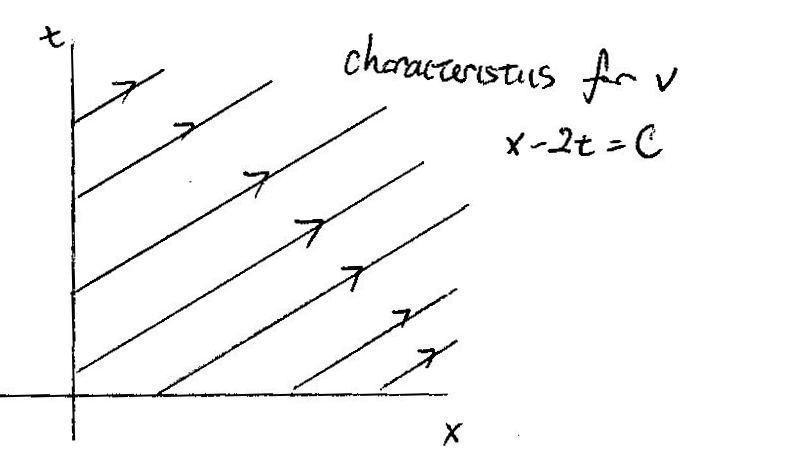
\includegraphics[scale = 0.5]{./_Figures/S098_1.png}
\end{center}
By how $v$ is defined, this corresponds to knowing data about $$u_{t}(x,0) + u_{x}(x, 0)$$ and $$u_{t}(0, t) + u_{x}(0,t).$$
Given $v$, the characteristics for $u_{t} + u_{x} = v$ imply that to solve for $v$, we need to know data about $u(x, 0)$ and $u(0, t)$.
\begin{center}
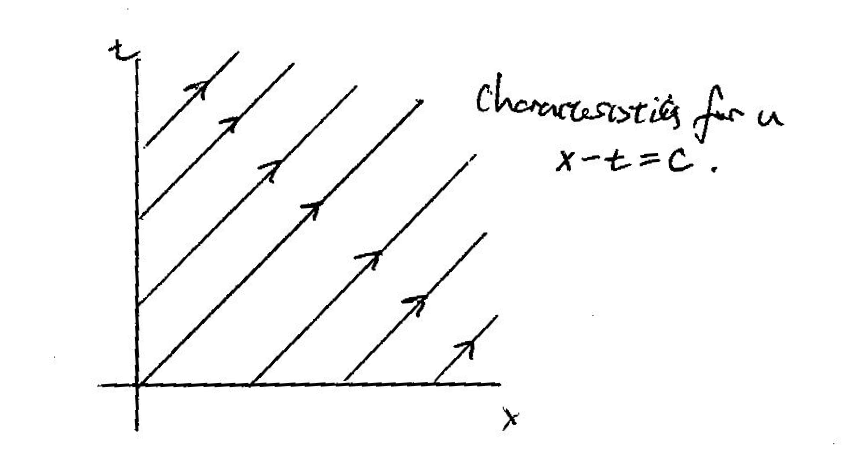
\includegraphics[scale=0.5]{./_Figures/S098_2.png}
\end{center}
Now suppose $u_{tt} + 3u_{xt} + 2u_{xx} = 0$ with
\begin{align*}
u(x,0) &= 0\\
u(0, t) &= 0\\
u_{t}(x, 0) + u_{x}(x, 0) &= 0\\
u_{t}(0, t) + u_{x}(0, t) &= 0.
\end{align*}
Since $v$ is constant on characteristics and $v(x, 0) = v(0, t) = 0$, we have $v = 0$. Since $u(x, 0) = u(0, t) = 0$ and $u$ is constant on characteristics,
$u = 0$. Moreover since the solution is constant on characteristics and we know the values of $u$ when the characteristics hit the $x$ and $t$ axes,
the characteristics uniquely determines the solution and hence $u = 0$ is the unique solution for the boundary value problem.
\hfill\qed

\subsection*{Solution to Spring 2009, \#9}\label{s099}
\subsubsection*{Solution to $(a)$}
Let $E[u] := \frac{1}{2}\int_{D}\abn{\nabla u}^{2}\, dx - \int_{\pr D}(f - \frac{a}{2}u)u\, d\sigma$. Then the minimizer $u$ satisfies
\begin{align*}
0 & = \lim_{\vep \rightarrow 0}\frac{1}{\vep}(E[u + \vep v] - E[u])\\
&= \lim_{\vep \rightarrow 0}\frac{1}{\vep}\bigg(\frac{1}{2}\int_{D}\abn{\nabla u + \vep \nabla v}^{2}\, dx \\
&\hspace{1in}- \int_{\pr D}(f - \frac{a}{2}u - \frac{a}{2}\vep v)(u + \vep v)\, d\sigma - \frac{1}{2}\int_{D}|\nabla u|^{2}\, dx + \int_{\pr D}(f - \frac{a}{2}u)u\, d\sigma\bigg)\\
&= \int_{D}\nabla u \cdot \nabla v\, dx - \int_{\pr D}fv - auv\, d\sigma\\
&= \int_{D}\nabla u \cdot \nabla v\, dx - \int_{\pr D}(f - au)v\, d\sigma\\
&= -\int_{D}\Delta u v\, dx + \int_{\pr D}\bigg(\frac{\pr u}{\pr n} - f + au\bigg)v\, d\sigma
\end{align*}
for all $v$. Then $\Delta u = 0$ in $D$ and $\frac{\pr u}{\pr n} + au = f$ on $\pr D$.
\hfill\qed

\subsubsection*{Solution to $(b)$}
Suppose there were two smooth solutions $u, v$. Let $w:= u - v$. Then
$\Delta w = 0$ in $D$ and $\frac{\pr w}{\pr n} + aw = 0$ on $\pr D$. Thus
\begin{align*}
0 = \int_{D}w\Delta w\, dx = -\int_{D}\abn{\nabla w}^{2}\, dx + \int_{\pr D}\frac{\pr w}{\pr n}w\, d\sigma = \int_{D}\abn{\nabla w}^{2}\, dx - \int_{\pr D}aw^{2}\, d\sigma.
\end{align*}
Since we also are given $a(x) > 0$, we have $\int_{D}\abn{\nabla w}^{2}\, dx \leq 0$. Therefore $w$ is a constant on $D$ and hence $w = 0$. Therefore if a smooth solution exists,
it is unique.
\hfill\qed


\section{Fall 2008}\label{f08}
\noindent The solution to Fall 2008, \#6 is the same as that of Spring 2008, \#3, see the solution to the Spring 2008 exam.

\sub{Solution to Fall 2008, \#1}\label{f081}
\ssb{Solution to $(a)$}
The minimizer $u$ satisfies
\ba
0 &= \lim_{\vep \rightarrow 0}\frac{1}{\vep}(J[u + \vep v] - J[u])\\
&= \lim_{\vep \rightarrow 0}\frac{1}{\vep}(\int_{\Om}|\del u + \vep\del v|^{2} + fu + f\vep v\, dx \\
&\hspace{1in}+ \int_{\Gamma}g(u + \vep v)^{2}\, d\sigma - \int_{\Om}(|\del u|^{2} + fu)\, dx - \int_{\Gamma}gu^{2}\, d\sigma)\\
&= \int_{\Om}2\del u \cdot \del v + fv\, dx + \int_{\Gamma}2guv\, d\sigma\\
&= 2(\int_{\Om}\del u \cdot \del v + \frac{f}{2}v \, dx+ \int_{\Gamma} guv\, d\sigma)\\
&= 2\bigg(-\int_{\Om}\lap u v - \frac{f}{2}v \, dx+ \int_{\Gamma}(\frac{\pr u}{\pr n} + gu)v\, d\sigma\bigg)
\ea
for all smooth compactly supported $v$.
Thus the minimizer satisfies
\ba
\lap u &= f/2 & &\text{in } \Om\\
\frac{\pr u}{\pr n} + gu &= 0 & &\text{on } \Gamma.
\ea
\hq

\ssb{Solution to $(b)$}
Assume $g(x) > 0$ on $\Gamma$. Let $U, v$ be two distinct solutions. Let
$w := u - v$. Then
\ba
-\lap w &= 0 && \text{in } \Om\\
\frac{\pr w}{\pr n} + gw &= 0 && \text{in } \Gamma.
\ea
We have
\ba
0 = \int_{\Om}w\lap w\, dx = -\int_{\Om}|\del w|^{2}\, dx + \int_{\Gamma}\frac{\pr w}{\pr n}w\, d\sigma = -\int_{\Om}|\del w|^{2}\, dx + \int_{\Gamma}-g w^{2}\, d\sigma.
\ea
Therefore $$-\int_{\Om}\abn{\del w}^{2}\, dx = \int_{\Gamma}gw^{2}\, d\sigma \geq 0.$$
Thus $\nms{\del w}_{L^{2}} = 0$ and hence $w$ is a constant in $\Om$ and by the given boundary conditions,
we have $w = 0$ in $\Om$.
\hq

\sub{Solution to Fall 2008, \#2}\label{f082}
We want to solve
\ba
u_{t} - u_{xx} &= 0 & & \text{in } \R^{+} \times (0, \infty)\\
u &= 0 && \text{on } \R^{+} \times \{t = 0\}\\
u &= g && \text{on } \{x = 0\} \times [0, \infty).
\ea
Let $v(x, t) = u(x, t) - g(t)$. Let
\ba
\wt{v}(x, t) = \begin{cases}
v(x, t) & \text{if } x \geq 0\\
-v(-x, t) & \text{if } x < 0.
\end{cases}
\ea
Then since
$$\frac{\pr^{2}}{\pr x^{2}}(-v(-x, t)) = \frac{\pr}{\pr x}(v_{x}(-x, t)) = -v_{xx}(-x, t),$$
we have
\ba
\wt{v}_{t} - \wt{v}_{xx} &= f(x, t) && \text{in } \R \times (0, \infty)\\
\wt{v}(x, 0) &= 0 && \text{on } \R^{+} \times \{t = 0\}\\
\wt{v}(0, t) &= 0 && \text{on } \{x = 0\} \times [0, \infty)
\ea
where
\ba
f(x, t) =
\begin{cases}
-g'(t) & \text{if } x \geq 0\\
g'(t) & \text{if } x < 0.
\end{cases}
\ea
Thus
\ba
\wt{v}(x, t) &= \int_{0}^{t}\frac{1}{\sqrt{4\pi(t - s)}}\int_{\R}e^{-\frac{\abn{x - y}^{2}}{4(t - s)}}f(y, s)\, dy\, ds\\
& = \int_{0}^{t}\frac{1}{\sqrt{4\pi(t - s)}}\int_{0}^{\infty}-e^{-\frac{\abn{x - y}^{2}}{4(t - s)}}g'(s)\, dy + \int_{-\infty}^{0}e^{-\frac{\abn{x - y}^{2}}{4(t - s)}}g'(s)\, dy\, ds\\
& = \int_{0}^{t}\frac{g'(s)}{\sqrt{4\pi(t - s)}}\bigg(\int_{-\infty}^{0}e^{-\frac{\abn{x - y}^{2}}{4(t - s)}}\, dy - \int_{0}^{\infty}e^{-\frac{\abn{x - y}^{2}}{4(t - s)}}\, dy\bigg)\, ds.
\ea
Then
\ba
u(x, t) = g(t) + \int_{0}^{t}\frac{g'(s)}{\sqrt{4\pi(t - s)}}\bigg(\int_{0}^{\infty}e^{-\frac{\abn{x + y}^{2}}{4(t - s)}} - e^{-\frac{\abn{x - y}^{2}}{4(t - s)}}\, dy\bigg)\, ds.
\ea
\hq

\sub{Solution to Fall 2008, \#3}\label{f083}
We first solve by method of characteristics. We have $$F(p, q, z, x, r) = q + zp.$$
Then
\ba
\dot{x} &= z && x(0) = x_0\\
\dot{t} &= 1 && t(0) = 0\\
\dot{z} &= 0 && z(0) = g(x_0).
\ea
Then $z(s) = g(x_0)$, $t(s) = s$, and $x(s) = g(x_0)s + x_0$.
The characteristics are given by $x = g(x_0)t + x_{0}$. Thus
if $x_0 > 1$, then $x = x_0$. If $x_0 < 0$, then $t = x - x_0$ which implies $x_0 = x - t$.
If $0 < x_0 < 1$, then $t = (x - x_0)/(1 - x_0)$ and hence $x_0 = (x - t)/(1 - t)$.
\begin{center}
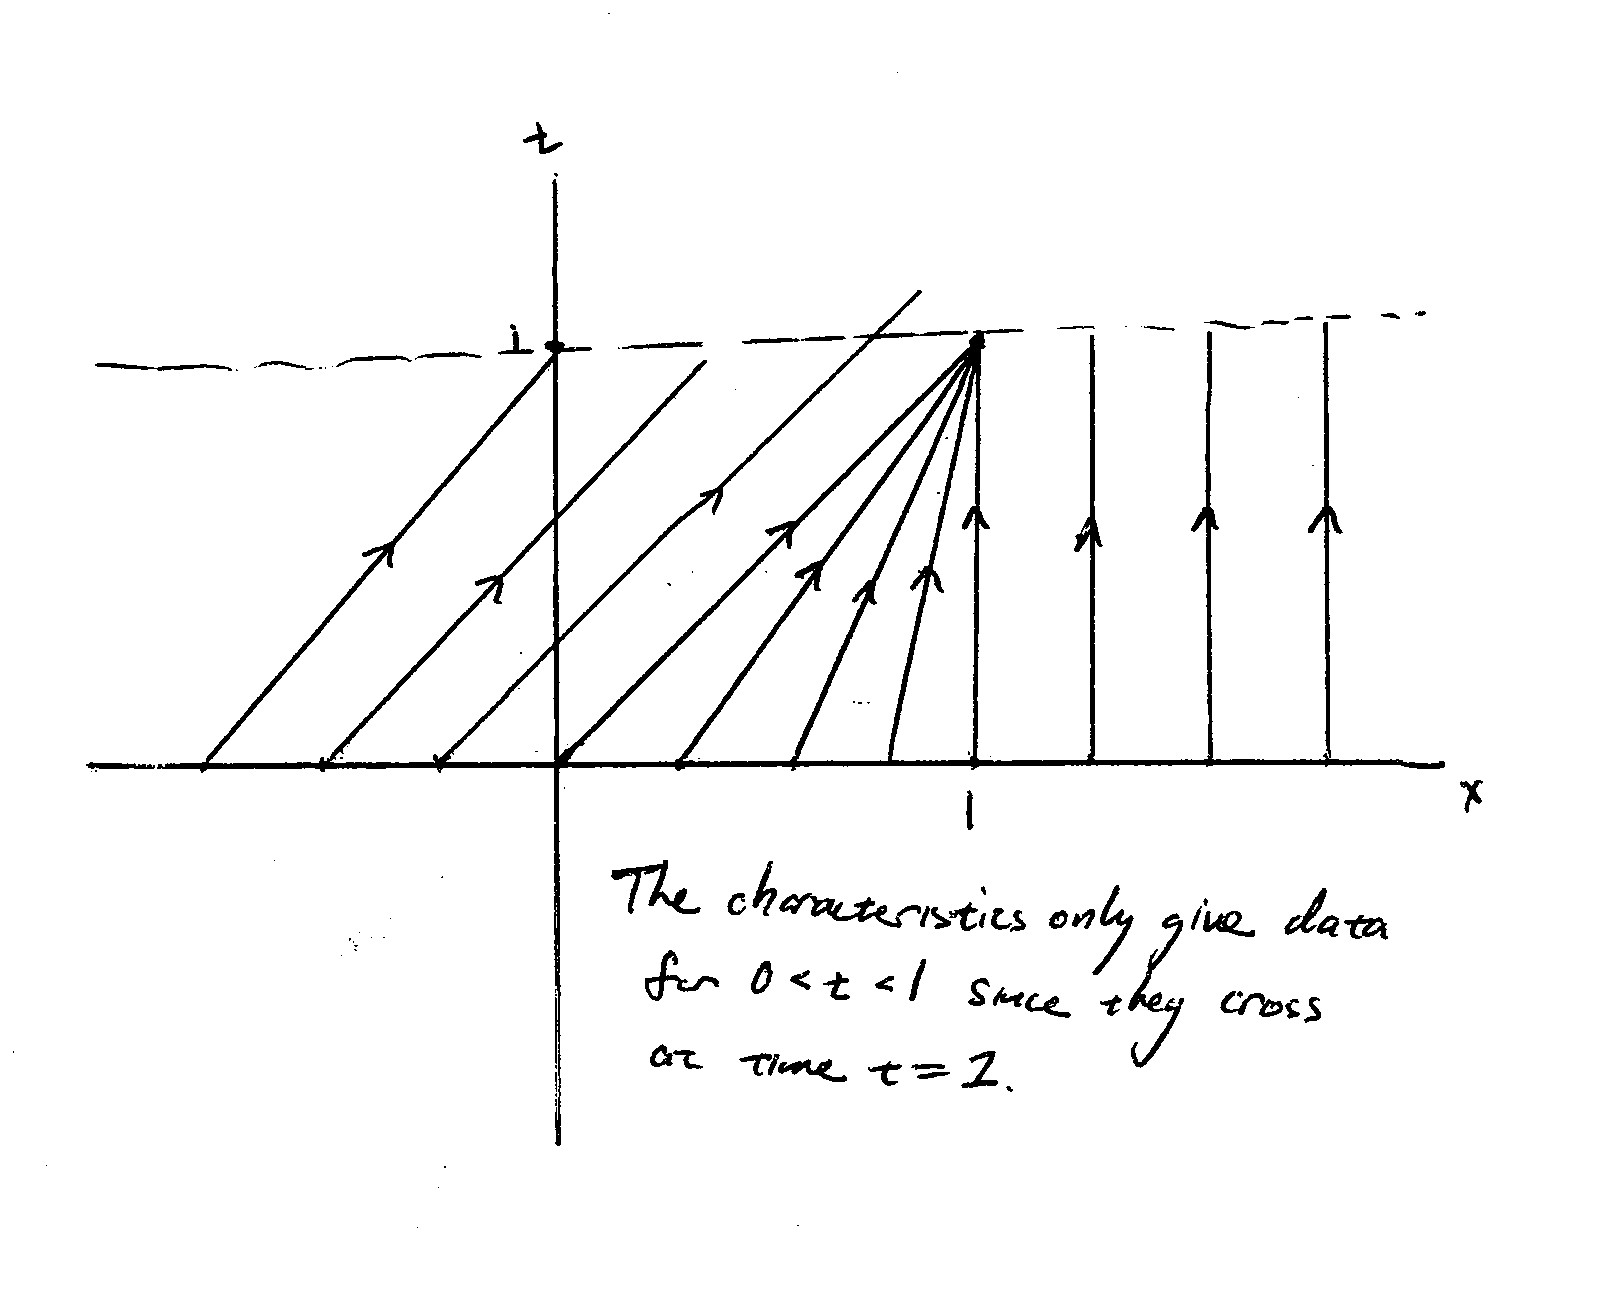
\includegraphics[scale=0.8]{./_Figures/F08Q3.jpg}
\end{center}
The characteristics cross at time $t = 1$ and hence for $t < 1$, the solution is given by
\ba
u(x, t) = \begin{cases}
0 & \text{ if } x > 1\\
1 - \frac{x - t}{1 - t} = \frac{1 - x}{1 - t} & \text{ if } 0 < \frac{x - t}{1 - t} < 1 \text{ (which happens if and only if $t < x < 1$)}\\
1 & \text{ if } x - t < 0 \text{ (which happens if and only if $x < t$)}.
\end{cases}
\ea
Since the characteristics cross, now we compute the shock curve $x = s(t)$. We have
$f(u) = (1/2)u^2$ and
$$\dot{s}(t) = \frac{f(1) - f(0)}{1 - 0}\quad \text{ with }\quad s(1) = 1.$$
Thus $\dot{s}(t) = 1/2$, $s(1) = 1$ which implies $s(t) = (t + 1)/2$. Therefore for $t > 1$, the entropy solution is
\ba
u(x, t) = \begin{cases}
1 & \text{ if } x < \frac{1}{2}(t + 1)\\
0 & \text{ if } x > \frac{1}{2}(t + 1).
\end{cases}
\ea
\hq

\sub{Solution to Fall 2008, \#4}\label{f084}
There is a rigorous argument in Evans. We will proceed nonrigorously. Let $\eta = x - ct$. Then $u_t = u_{xx} + 1 - u^2$ becomes
$-cf' = f'' + 1 - f^2$. Writing this as a system gives that we need to analyze
\ba
x' &= y\\
y' &= -cy - 1 + x^2.
\ea
The stationary points are $(1, 0)$ and $(-1, 0)$.
The Jacobian is $J(x, y) = \smat{0}{1}{2x}{-c}$ and hence $J(1, 0) = \smat{0}{1}{2}{-c}$ and $J(-1, 0) = \smat{0}{1}{-2}{-c}$.
\begin{enumerate}[$(i)$]
\item $J(1, 0) = \smat{0}{1}{2}{-c}$: This matrix has eigenvalues $\ld = \frac{-c \pm \sqrt{c^2 + 8}}{2}$ and hence is a saddle
for all $c > 0$.
\item $J(-1, 0) = \smat{0}{1}{-2}{-c}$: This matrix has eigenvalues $\ld = \frac{-c \pm \sqrt{c^2 - 8}}{2}$ and hence
is a sink node if $c > 2\sqrt{2}$, a stable spiral if $c < 2\sqrt{2}$, and an improper node if $c = 2\sqrt{2}$.
\end{enumerate}
If $c < 2\sqrt{2}$, then $(-1, 0)$ is a spiral and so that there are times for which $y > 0$.
Since $y = x'$, we have that $x$ is not monotonically decreasing when $c < 2\sqrt{2}$. Translating this back to the problem,
we have shown that $f$ is not monotonically decreasing when $c < 2\sqrt{2}$.

Let $\ld_{\pm} := \frac{-c \pm \sqrt{c^2 + 8}}{2}$. Note that $\smat{0}{1}{2}{-c}\svt{a}{b} = \ld_{\pm}\svt{a}{b}$ implies
$b = \ld_{\pm}a$. Thus the eigenvectors for this eigenvalue is $$\vct{1}{\ld_{\pm}} = \vct{1}{\frac{-c \pm \sqrt{c^2 + 8}}{2}}$$
and so locally near $(1, 0)$, the phase plane looks like
\begin{center}
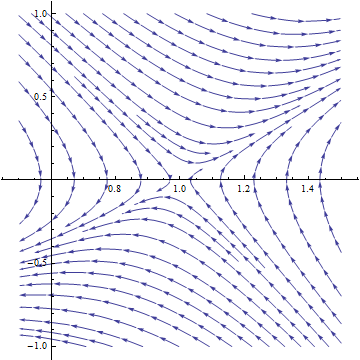
\includegraphics[scale=0.75]{./_Figures/F08Q4.png}
\end{center}
Since $(-1, 0)$ is either a stable spiral or a sink, then there exists a unique $f$ such that $\lim_{x \rightarrow -\infty}f(x) = 1$
and $\lim_{x \rightarrow \infty}f(x) = -1$.
\hq

\sub{Solution to Fall 2008, \#5}\label{f085}
We want to show that
\ba
\int_{\R^3}-\frac{1}{4\pi}\int_{\R^3}\frac{f(y)}{|x - y|}\, dy \lap \phi(x)\, dx = \int_{\R^3}f(x)\phi(x)\, dx.
\ea
By Fubini's Theorem,
\ba
\int_{\R^3}f(y)\int_{\R^3}-\frac{1}{4\pi|x - y|}\lap \phi(x)\, dx\, dy = \int_{\R^3}f(y)\phi(y)\, dy.
\ea
Thus it suffices to prove that for each $x \in \R^3$,
$$\phi(x) = \int_{\R^3}\lap_{y}\phi(y)(-\frac{1}{4\pi\abn{y - x}})\, dy.$$
We have
\ba
\int_{\R^3}\lap_{y}\phi(y)(-&\frac{1}{4\pi\abn{y - x}})\, dy = \int_{\R^3}(-\lap_{y}\phi)(x - y)\frac{1}{4\pi\abn{y}}\, dy\\
&=\int_{B(0, \vep)}(-\lap_{y}\phi)(x - y)\frac{1}{4\pi\abn{y}}\, dy + \int_{\R^3\bs B(0, \vep)}(-\lap_{y}\phi)(x - y)\frac{1}{4\pi\abn{y}}\, dy.
\ea
Observe that
\ba
\abb{\int_{B(0, \vep)}(-\lap_{y}\phi)(x - y)\frac{1}{4\pi\abn{y}}\, dy} &\lsm \nms{\lap \phi}_{L^{\infty}}\int_{B(0, \vep)}\frac{1}{\abn{y}}\, dy\\
 &\lsm \abn{\lap\phi}_{L^{\infty}}\int_{0}^{\vep}\frac{1}{r}r^2\, dr \lsm \nms{\lap\phi}_{L^{\infty}}\vep^{2} \rightarrow 0
\ea
as $\vep \rightarrow 0$
and with $\kap(y) = -\frac{1}{4\pi\abn{y}}$,
\ba
\int_{\R^3\bs B(0, \vep)}&(-\lap_{y}\phi)(x - y)\frac{1}{4\pi\abn{y}}\, dy = \int_{\R^3\bs B(0, \vep)}\lap_{y}\phi(x - y)\kap(y)\, dy\\
&=\int_{\R^3 \bs B(0, \vep)}\phi(x - y)\lap\kap(y)\, dy + \int_{\pr(\R^3\bs B(0, \vep))}-\phi(x - y)\frac{\pr\kap}{\pr \nu} + \kap(y)\frac{\pr\phi}{\pr\nu}(x - y)\, d\sigma.
\ea
Since $\lap\kap = 0$ on $\R^3 \bs B(0, \vep)$ and
\ba
\int_{\pr(\R^3 \bs B(0, \vep))}\kap(y)\frac{\pr\phi}{\pr\nu}(x - y)\, d\sigma \lsm \nms{\del \phi}_{L^{\infty}}\int_{\pr B(0, \vep)}\frac{1}{\abn{y}}\, d\sigma \lsm \vep\nms{\del \phi}_{L^{\infty}} \rightarrow 0
\ea
as $\vep \rightarrow \infty$ we have
\ba
\int_{\R^3}\lap_{y}\phi(y)(-\frac{1}{4\pi\abn{y - x}})\, dy = \lim_{\vep \rightarrow 0}\int_{\pr(\R^3\bs B(0, \vep))}\phi(x - y)\frac{\pr \kap}{\pr\nu}\, d\sigma.
\ea
Since $\del \kap(y) = \frac{1}{4\pi}\frac{y}{\abn{y}^3}$ and $\nu = -y/\abn{y}$, we have
$$\frac{\pr \kap}{\pr\nu} = -\frac{1}{4\pi}\frac{\abn{y}^{2}}{\abn{y}^4} = -\frac{1}{4\pi}\frac{1}{\abn{y}^2}.$$
Then
\ba
\int_{\pr(\R^3\bs B(0, \vep))}-\phi(x - y)\frac{\pr \kap}{\pr \nu}\, d\sigma &= \frac{1}{4\pi\vep^2}\int_{\pr B(0, \vep)}\phi(x - y)\, d\sigma(y)\\
 &= \frac{1}{4\pi\vep^2}\int_{\pr B(x, \vep)}\phi(y)\, d\sigma(y) \rightarrow \phi(x)
\ea
as $\vep \rightarrow 0$. This shows that
$$\phi(x) = -\frac{1}{4\pi}\int_{\R^3}\frac{\lap \phi(y)}{\abn{x - y}}\, dy.$$

\begin{rem}
Alternatively, $-\frac{1}{4\pi\abn{x}}$ is the fundamental solution of the Laplacian.
Let $v(x) := -\frac{1}{4\pi}\int_{\R^3}\frac{\lap \phi(y)}{\abn{x - y}}\, dy$. Then
$\lap(v - \phi) = 0$ in $\R^3$. Since $\phi, v \rightarrow 0$ as $\abn{x} \rightarrow \infty$,
it follows that $v = \phi$. \hq
\end{rem}

\sub{Solution to Fall 2008, \#7}\label{f087}
We have
$$\int_{0}^{1}uu_{xxt} + uu_{xx} - u^{4}\, dx = 0$$
and hence
$$-\int_{0}^{1}u_{x}u_{xt}\, dx - \int_{0}^{1}u_{x}^{2}\, dx - \int_{0}^{1}u^{4}\, dx = 0.$$
Let $$w(t) := \int_{0}^{1}u_{x}^{2}\, dx.$$
Then $w'(t) = \int_{0}^{1}2u_{x}u_{xt}\, dx$. Thus
$$-\frac{1}{2}w'(t) - w(t) = \int_{0}^{1}u^{4}\, dx \geq 0$$
which implies
$$\frac{1}{2}w'(t) + w(t) \leq 0$$
and hence
$$(e^{2t}w(t))' \leq 0.$$
Thus $e^{2t}w(t)$ is monotonically decreasing. Then
$e^{2t}w(t) \leq w(0)$ which after rearranging gives
$$w(t) \leq e^{-2t}w(0).$$
Since
$$w(0) = \int_{0}^{1}(u_{x})^{2}(x, 0)\, dx = \int_{0}^{1}(2x - 1)^{2}\, dx = \frac{1}{3},$$
we have
$$0 \leq w(t) \leq \frac{1}{3}e^{-2t}.$$
Thus
\ba
\abn{u(y, t)} = \abb{\int_{0}^{y}u_{x}(x, t)\, dx} \leq \bigg(\int_{0}^{1}\abn{u_{x}(x, t)}^{2}\, dx\bigg)^{1/2} \leq \frac{e^{-t}}{\sqrt{3}} \rightarrow 0
\ea
as $t \rightarrow \infty$.
\hq

\sub{Solution to Fall 2008, \#8}\label{f088}
By Sturm-Liouville theory, the smallest $\ld$ for the eigenvalue problem $$u'' - q(x)u = -\ld u$$
is given by
$$\ld = \min_{u: u'(0) = u'(1) = 0}\frac{\ips{u, Lu}}{\ips{u, u}}.$$
Pick a smooth compactly supported function $u_{0}$ such that
$u_{0}'(0) = u_{0}'(1) = 0$ and $\int_{0}^{1}qu_{0}\, dx \neq 0$. Consider
$\ips{u_{0} + c, L(u_{0} + c)}$ for some $c$ to be chosen later. We have
\ba
\ips{u_{0} + c, &L(u_{0} + c)} = \ips{u_{0} + c, Lu_{0} + Lc} = \ips{u_{0}, Lu_{0}} + \ips{u_{0}, Lc} + c\ips{1, Lu_{0}} + \ips{c, Lc}\\
& = \ips{u_{0}, Lu_{0}} + c\int_{0}^{1}u_{0}q\, dx + c\int_{0}^{1}-u_{0}'' + qu_{0}\, dx = \ips{u_{0}, Lu_{0}} + 2c\int_{0}^{1}u_{0}q\, dx.
\ea
Now choose $c$ such that $\ips{u_{0}, Lu_{0}} + 2c\int_{0}^{1}u_{0}q\, dx < 0$. Then with this choice of $c$,
\ba
\ld = \min_{u: u'(0) = u'(1) = 0}\frac{\ips{u, Lu}}{\ips{u, u}} \leq \frac{\ips{u_{0} + c, L(u_{0} + c)}}{\ips{u_{0} + c, u_{0} + c}} < 0.
\ea
\hq


\section{Spring 2008}\label{s08}
\subsection*{Solution to Spring 2008, \#1}\label{s081}
\subsubsection*{Solution to $(a)$}
We have
\begin{align*}
(f'(x)g(x) - g'(x)f(x))_{x = 0}^{\ell} &= f'(\ell)g(\ell) - g'(\ell)f(\ell) - f'(0)g(0) + g'(0)f(0)\\
&= f'(\ell)g(\ell) + g(\ell)f(\ell) = g(\ell)(f'(\ell) + f(\ell)) = 0.
\end{align*}
\hfill\qed

\subsubsection*{Solution to $(b)$}
Let $\ld_{1}$, $\ld_{2}$ be distinct nonzero eigenvalues corresponding to eigenfunctions $u_{1}, u_{2}$.
Then
\begin{align*}
\ld_{1}\int_{0}^{\ell}u_{1}u_{2}\, dx &= \int_{0}^{\ell}-u_{1}''u_{2}\, dx\\
&= -(u_2u_1' - u_2'u_1)_{x = 0}^{\ell} + \int_{0}^{\ell}u_{2}''u_{1}\, dx\\
&= -\int_{0}^{\ell}u_{2}''u_{1}\, dx = \ld_{2}\int_{0}^{\ell}u_{2}u_{1}\, dx.
\end{align*}
Therefore
$$(\ld_{1} - \ld_{2})\int_{0}^{\ell}u_{1}u_{2}\, dx = 0.$$
Since $\ld_{1} \neq \ld_{2}$, $\int_{0}^{\ell}u_{1}u_{2}\, dx = 0$.
\hfill\qed

\subsubsection*{Solution to $(c)$}
We claim that this problem has no eigenfunctions corresponding to $\ld = 0$.
Suppose $y$ is an eigenfunction corresponding to the eigenvalue $\ld = 0$.
Then
$$y'' = 0, \quad y'(\ell) + y(\ell) = 0, \quad y(0) = 0.$$
Therefore $y(x) = ax + b$. Since $y(0) = 0$, $b = 0$. Thus $y = ax$. Since $y'(\ell) + y(\ell) = 0$,
$a + a\ell = 0$ and hence $a = 0$. Therefore $y$ is the zero function.
This contradicts that $y$ is an eigenfunction.

Suppose $\ld < 0$. Then $\ld = -\mu$, $\mu > 0$.
We have
$$y'' - \mu y = 0, \quad y'(\ell) + y(\ell) = 0, \quad y(0) = 0.$$
Thus the general solution is
$$y(x) = Ae^{\sqrt{\mu}x} + Be^{-\sqrt{\mu}x}.$$
As $y(0) = 0$, $A + B = 0$. We have
$$y'(x) = A\sqrt{\mu}e^{\sqrt{\mu}x} - B\sqrt{\mu}e^{-\sqrt{\mu}x}.$$
Thus using $y'(\ell) + y(\ell) = 0$ gives
\begin{align*}
A\sqrt{\mu}e^{\sqrt{\mu}\ell} - B\sqrt{\mu}e^{-\sqrt{\mu}\ell} + Ae^{\sqrt{\mu}\ell} + Be^{-\sqrt{\mu}\ell} &= 0\\
Ae^{\sqrt{\mu}\ell}(\sqrt{\mu} + 1) + Be^{-\sqrt{\mu}\ell}(1 - \sqrt{\mu}) &= 0.
\end{align*}
Since $A = -B$, we have
$$A(e^{\sqrt{\mu}\ell}\sqrt{\mu} + e^{\sqrt{\mu}\ell} - e^{-\sqrt{\mu}\ell} + \sqrt{\mu}e^{-\sqrt{\mu}\ell}) = 0.$$
If $A = 0$, then $B = 0$, so assume $A \neq 0$ since we want nontrivial solutions. Then
\begin{align}\label{s08beq1}
e^{\sqrt{\mu}\ell}\sqrt{\mu} + e^{\sqrt{\mu}\ell} - e^{-\sqrt{\mu}\ell} + \sqrt{\mu}e^{-\sqrt{\mu}\ell} = 0
\end{align}
and we want to solve for $\sqrt{\mu}$. Let $\alpha := \sqrt{\mu}$. Then
\begin{align*}
\alpha e^{\alpha \ell} + e^{\alpha\ell} - e^{-\alpha \ell} + \alpha e^{-\alpha \ell} &= 0\\
e^{\alpha\ell}(\alpha + 1) + e^{-\alpha\ell}(\alpha - 1) &= 0.
\end{align*}
Let $f(t) := e^{\ell t}(t + 1) + e^{-\ell t}(t - 1)$. Note that $f(0) = 0$.
Since
\begin{align*}
f'(t) &= \ell e^{\ell t}(t + 1) + e^{\ell t} - \ell e^{-\ell t}(t - 1) + e^{-\ell t}\\
&= \ell e^{\ell t}(t + 1) + e^{\ell t} + e^{-\ell t} + \ell e^{-\ell t} - t\ell e^{-\ell t}\\
&> \ell(t + 1) + 1 + 1 + \ell - t\ell > 0.
\end{align*}
Therefore there are no solutions to \eqref{s08beq1}. Thus there are no eigenfunctions in this case.

Finally, let $\ld > 0$. In this case, the general solution is
$$y(x) = A\cos(\sqrt{\ld}x) + B\sin(\sqrt{\ld}x).$$
Since $y(0) = 0$, $A = 0$ and hence $y(x) = B\sin(\sqrt{\ld}x)$ and $y'(x) = B\sqrt{\ld}\cos(\sqrt{\ld}x).$
Since $y'(\ell) + y(\ell) = 0$,
$$B\sqrt{\ld}\cos(\sqrt{\ld}\ell) + B\sin(\sqrt{\ld}\ell) = 0.$$
Since we want nontrivial solutions, assume $B \neq 0$. Then
$$\sqrt{\ld}\cos(\sqrt{\ld}\ell) + \sin(\sqrt{\ld}\ell) = 0.$$
Simplifying gives
$$\tan(\sqrt{\ld}\ell) = -\sqrt{\ld}.$$
This equation has infinitely many positive solutions.
\hfill\qed

\subsection*{Solution to Spring 2008, \#2}\label{s082}
We use method of characteristics. We have $F(p, q, z, x, y) = p^{2} + q^{2} + 1$ and
\begin{align*}
\begin{array}{ll}
\dot{x} = 2p & x(0) = x_{0}\\
\dot{y} = 2q & y(0) = y_{0}\\
\dot{z} = 2 & z(0) = 1\\
\dot{p} = 0 & p(0) = p_{0}\\
\dot{q} = 0 & q(0) = q_{0}
\end{array}
\end{align*}
where $x_{0}^{2} + y_{0}^{2} = 1$ and $p_{0}^{2} + q_{0}^{2} = 1$.
Since $u_{\ta} = 0$ on $\Gamma$ and
$$u_{\ta} = -u_{x}\sin\ta + u_{y}\cos\ta \quad \text{ for $r = 1$},$$
we have
$$0 = -p_{0}y_{0} + q_{0}x_{0}.$$
Therefore $(p_{0}, q{0})$ is orthogonal to $(-y_{0}, x_{0})$. Since $(x_{0}, y_{0})$
is orthogonal to $(-y_{0}, x_{0})$, $(x_{0}, y_{0})$ and $(p_{0}, q_{0})$ are parallel.
Then $$(x_{0}, y_{0}) \cdot (p_{0}, q_{0}) = \pm\nms{(x_{0}, y_{0})}\nms{(p_{0}, q_{0})} = \pm 1.$$
We have
\begin{align*}
x(s) &= 2p_{0}s + x_{0}\\
y(s) &= 2q_{0}s + y_{0}\\
z(s) &= 2s + 1.
\end{align*}
Since $x_{0}p_{0} + y_{0}q_{0} = \pm 1$,
$$x^{2} + y^{2} = 4p_{0}^{2}s^{2} + 4p_{0}sx_{0} + x_{0}^{2} + 4q_{0}^{2}s^{2} + 4q_{0}sy_{0} + y_{0}^{2} = 4s^{2} \pm 4s + 1.$$
If we had $x^{2} + y^{2} = 4s^{2} + 4s + 1$, then $x^{2} + y^{2} = z^{2}$ and hence
$z = \pm \sqrt{x^{2} + y^{2}}$. Since $z(0) = 1$, it follows that $u(x, y) = \sqrt{x^{2} + y^{2}}$.
On the other hand if we had $x^{2} + y^{2} = 4s^{2} - 4s + 1 = (2s - 1)^{2} = (z - 2)^{2}$
and hence $z = 2 \pm \sqrt{x^{2} + y^{2}}$. Since $z(0) = 1$, it follows that $u(x, y) = 2 - \sqrt{x^{2} + y^{2}}$.
Thus we have two solutions, $u(x, y) = \sqrt{x^{2} + y^{2}}$ and $u(x, y) = 2 - \sqrt{x^{2} + y^{2}}$.
\hfill\qed

\subsection*{Solution to Spring 2008, \#3}\label{s083}
This problem is the same as Fall 2008, \#6.

\vspace{0.4cm}

We first show that, given initial data with compact support, solutions to the PDE also have compact support. With this, we can then easily prove that the solution is unique. Define
$$ \Lambda := \max_{|\xi|=1,\,\, 1 \leq l \leq m} |\lambda_l(\xi)| $$
where $\lambda_l (\xi)$ for $l = 1, 2, \dots, m$ are the eigenvalues of the matrix $A(\xi) = \sum_{j=1}^n \xi_j A_j$. Note that $\xi \in \R^n$, and $\xi_j$ is the $j$th component of $\xi$. Because each $A_j$ is an $m \times m$ symmetric matrix, $A(\xi)$ is also an $m \times m$ symmetric matrix for all $\xi$, so $\Lambda$ is well-defined and real.

\vspace{0.2cm}

Now, we claim that, if $u = 0$ on $B(x_0,t_0) \times \{t = 0\}$, then $u \equiv 0$ within the cone $$ K(x_0,t_0) := \{ (x,t) \, : \, 0 \leq t \leq t_0, \,\, |x-x_0| \leq \Lambda(t_0 - t)\}$$
To this end, fix $(x_0,t_0)$ so that $u=0$ on $B(x_0,t_0) \times \{t=0\}$. This is possible because $u(x,0) = f(x)$ has compact support. Now, consider the energy
$$ E(t) := \frac{1}{2} \int_{B(x_0, \Lambda(t_0-t))} |u|^2 \, dx $$
Differentiating the energy with respect to $t$ yields
\begin{align*}
	E'(t) &= \int_{B(x_0, \Lambda(t_0-t))} u \cdot u_t \, dx - \frac{\Lambda}{2} \int_{\d B(x_0, \Lambda(t_0-t))} |u|^2 \, dS(x) \\
	&= -\int_{B(x_0, \Lambda(t_0-t))} u \cdot \sum_{i=1}^n A_i u_{x_i} \, dx - \frac{\Lambda}{2} \int_{\d B(x_0, \Lambda(t_0-t))} |u|^2 \, dS(x)
\end{align*}
We're going to \emph{carefully} apply integration by parts. Fix $1 \leq k \leq n$. We compute
$$ \int_{B(x_0, \Lambda(t_0-t))} u \cdot A_k u_{x_k} \, dx = \int_{\d B(x_0, \Lambda(t_0-t))} u \cdot A_k u \nu^k \, dx - \int_{B(x_0, \Lambda(t_0-t))} u_{x_k} \cdot A_k u \, dx $$
where $\nu^k$ is the $k$th component of the outward unit normal $\nu$. Because $A_k$ is symmetric, $u \cdot A u_{x_k} = u_{x_k} \cdot A u$, so we obtain
$$ \int_{B(x_0, \Lambda(t_0-t))} u \cdot A_k u_{x_k} \, dx = \frac{1}{2} \int_{\d B(x_0, \Lambda(t_0-t))} u \cdot A_k u \nu^k \, dx $$
Hence,
\begin{align}
\label{s08energy}
	 E'(t) &= -\frac{1}{2} \int_{\d B(x_0, \Lambda(t_0-t))} u \cdot \sum_{i=1}^n \nu^i A_i u \, dx - \frac{\Lambda}{2} \int_{\d B(x_0, \Lambda(t_0-t))} |u|^2 \, dS(x) \\
\label{s08nrgysimp}	  &= \frac{1}{2} \int_{\d B(x_0, \Lambda(t_0-t))} u \cdot A(\nu) u \, dx - \frac{\Lambda}{2} \int_{\d B(x_0, \Lambda(t_0-t))} |u|^2 \, dS(x)
\end{align}
Note that the negative sign that was originally attached to the first integral of \eqref{s08energy} above was absorbed into the definition of $A(\nu)$ since $-\nu$ is still a unit vector. Finally, recall that we can obtain the maximum eigenvalue of a symmetric matrix by maximizing the Rayleigh quotient. Thus, by our definition of $\Lambda$, we have
$$ \frac{u \cdot A(\nu) u}{u \cdot u} \leq \Lambda \quad \implies \quad u \cdot A(\nu) u \leq \Lambda |u|^2 $$
Applying this to \eqref{s08nrgysimp} yields $E'(t) \leq 0$. Furthermore, because of how we picked $(x_0,t_0)$, $E(0)=0$. Thus, since $E(t)$ is nonnegative for all $t > 0$, we have $E(t) \equiv 0$ for $0 \leq t \leq t_0$. Therefore, we have shown that $u \equiv 0$ in the cone $K(x_0,t_0)$. This implies that, given initial data that is compactly supported, solutions to the PDE will also be compactly supported.

\vspace{0.2cm}

Now, we can prove that the solution to the PDE is unique. Suppose $u$ and $v$ are both solutions to the PDE. Then, by linearity, $w :=u-v$ also satisfies the PDE with initial data $w(x,0) = 0$. Define
$$ E(t) := \frac{1}{2} \int_{\R^n} |w|^2 \, dx $$
and compute
$$ E'(t) = \int_{\R^n} w \cdot w_t \, dx = -\int_{\R^n} w \cdot \sum_{i=1}^n A_i w_{x_i} \, dx $$
Applying integration by parts and using the fact that $A_i$ is symmetric for all $i$ yields
$$ -\int_{\R^n} w \cdot \sum_{i=1}^n A_i w_{x_i} \, dx = \int_{\R^n} w \cdot \sum_{i=1}^n A_i w_{x_i} \, dx $$
Recall that $w$ is compactly supported from our work above, so the boundary integrals from integration by parts vanish. This implies that $E'(t) = 0$. Finally, we also know $E(0) = 0$, so by non-negativity of our energy, we have $E(t) \equiv 0$ for all time $t$. Hence, $w \equiv 0$, so $u=v$.
\hfill\qed

\subsection*{Solution to Spring 2008, \#4}\label{s084}
Observe that $u_{tt} + u_{xt} - 20u_{xx} = 0$ can be written as
$$(\pr_{t} - 4\pr_{x})(\pr_{t} + 5\pr_{x})u = 0.$$
Let $v := u_{t} + 5u_{x}$. Then
\begin{align*}
v_{t} - 4v_{x}  &= 0\\
v(x, 0) &= \psi(x) + 5\phi'(x).
\end{align*}
Thus
$$v(x, t) = \psi(x + 4t) + 5\phi'(x + 4t)$$
(where for clarity, $\phi'(x + 4t) = (\phi')(x + 4t)$, that is the function $\phi'$ evaluated at $x + 4t$).
Then
\begin{align*}
u_{t} + 5u_{x} &= \psi(x + 4t) + 5\phi'(x + 4t)\\
u(x, 0) &= \phi(x)
\end{align*}
and hence
\begin{align*}
u(x, t) &= \phi(x - 5t) + \int_{0}^{t}\psi(x + 5(s - t) + 4s) + 5\phi'(x + 5(s - t) + 4s)\, ds\\
&= \phi(x - 5t) + \frac{1}{9}\int_{x - 5t}^{x + 4t}\psi(s)\, ds + \frac{5}{9}\int_{x - 5t}^{x + 4t}\phi'(u)\, du\\
&= \frac{4}{9}\phi(x - 5t) + \frac{5}{9}\phi(x + 4t) + \frac{1}{9}\int_{x - 5t}^{x + 4t}\psi(s)\, ds.
\end{align*}
\hfill\qed

\subsection*{Solution to Spring 2008, \#5}\label{s085}
Let $f \in C_{c}^{\infty}(\R^{n})$. Then
$$(\Delta - aI)\int_{\R^{n}}K_{a}(x - y)f(y)\, dy = f(x)$$
and
$$(\Delta - bI)\int_{\R^{n}}K_{b}(x - y)f(y)\, dy = f(x).$$
Note that $(\Delta - aI)(\Delta - bI) = (\Delta - bI)(\Delta - aI).$
Thus
\begin{align}\label{s085eq1}
\begin{aligned}
(\Delta - aI)(\Delta - bI)\int_{\R^{n}}(c_{1}K_{a}(x - y) &+ c_{2}K_{b}(x - y))f(y)\, dy\\
&= c_{1}(\Delta - bI)f(x) + c_{2}(\Delta - aI)f(x).
\end{aligned}
\end{align}
Since we want $c_{1}K_{a} + c_{2}K_{b}$ to be a fundamental solution, we want the right hand
side of \eqref{s085eq1} to equal $f(x)$. This is satisfied when
\begin{align*}
c_{1} + c_{2} &= 0\\
bc_{1} + ac_{2} &= -1
\end{align*}
and hence $c_{1} = \frac{1}{a - b}$ and $c_{2} = -\frac{1}{a - b}.$
\hfill\qed

\subsection*{Solution to Spring 2008, \#6}\label{s086}
We use a Fourier series expansion. We have
\begin{align*}
\wh{u}_{t}(k, t) &= \vep k^{2}\wh{u}(k, t) + (ik)^{6}\wh{u}(k, t)\\
\wh{u}_{t}(k, t) &= (\vep k^{2} - k^{6})\wh{u}(k, t)\\
\wh{u}(k, t) &= e^{(\vep k^{2} - k^{6})t}\wh{u}(k, 0).
\end{align*}
Therefore
$$u(x, t) = \sum_{k \in \Z}e^{(\vep k^{2} - k^{6})t}\wh{u}(k, 0)e^{ikx}.$$
For the PDE to always stay bounded as $t \rightarrow \infty$, we need
$\vep k^{2} - k^{6} < 0$ for all $k \in \Z$, $k \neq 0$. Thus
$\vep < k^{4}$ for all $k \in \Z$, $k \neq 0$. Therefore
$\vep_{0} = 1$.
\hfill\qed

\subsection*{Solution to Spring 2008, \#7}\label{s087}
This is a good problem illustrating two major tricks: the first time argument and the $L^{p}$ trick.

\subsubsection*{Solution to $(a)$}
Fix a time interval of existence $[0, T]$.
Fix $\vep > 0$ small and let
$$v := u - \vep e^{(\beta/2)t}.$$
We have
\begin{align*}
v_{t} &= u_{t} - \frac{\beta \vep}{2}e^{(\beta/2)t}\\
\Delta v &= \Delta u\\
\beta u(1 - u) &= \beta (v + \vep e^{(\beta/2)t})(1 - v - \vep e^{(\beta/2)t}).
\end{align*}
Then
\begin{align*}
u_{t} &= \Delta u + \beta u(1 - u)\\
v_{t} + \frac{\beta \vep}{2}e^{(\beta/2)t} &= \Delta v + \beta (v + \vep e^{(\beta/2)t})(1 - v - \vep e^{(\beta/2)t}).
\end{align*}
Since $u(x, 0)$ is $ > 0$, if $\vep$ is made small enough, $v(x , 0) > 0$. Let
$t_{0}$ be the first time $v$ hits $0$, that is $v(x_{0}, t_{0}) = 0$.
Then $v_{t}(x_{0}, t_{0}) \leq 0$ and $\Delta v(x_{0}, t_{0}) \geq 0$
since $v(x, t') > 0$ for $t' < t_{0}$ and $v(x, t_{0}) \geq 0$. Then at $(x_{0}, t_{0})$,
\begin{align}\label{s087aeq1}
\frac{\beta\vep}{2}e^{(\beta/2)t_{0}} & \geq \beta(\vep e^{(\beta/2)t_{0}})(1 - \vep e^{(\beta/2)t_{0}})\nonumber\\
\frac{\vep}{2}e^{(\beta/2)t_{0}} & \geq \vep e^{(\beta/2)t_{0}} - \beta \vep^{2}e^{\beta t_{0}}.
\end{align}
This is a contradiction if $\vep$ is chosen to be sufficiently small. (Indeed, it suffices to choose
$\vep < \frac{1}{2\beta e^{\beta T}}$ which would imply $\frac{1}{2}e^{(\beta/2)t_{0}} > \beta \vep e^{\beta T}$
and hence contradict \eqref{s087aeq1}.) Therefore no such $(x_{0}, t_{0})$
exists and hence $v(x, t) > 0$ for all $x, t$. Thus $u(x, t) > \vep e^{(\beta/2)t}$ for all $x, t$.
\hfill\qed

\subsubsection*{Solution to $(b)$}
Without loss of generality we assume $T^{n} = [0, 1]^{n}$ (any other tori can be rescaled to the unit cube and hence will only change the constants
that appear in argument). The PDE is the Fisher-KPP equation. We will assume that $\beta > 0$. An apriori bound is a bound on $u$ assuming that $u$ exists (hence
the ``apriori" part).

We present two solutions,
the first solution is one that relies on the $L^{p}$ trick. This trick is more straightforward to start, however a bit more complicated (though routine) to finish.
The second solution is applying a certain transformation on the solution and then using the maximum principle, however this approach relies
on a clever substitution and the author only saw this upon finish the $L^{p}$ trick approach.\\

\noindent \textit{$L^{p}$-trick Solution:} Let $E(t) := \int_{T^{n}}u^{p}\, dx$ with $p$ large. (We are defining $E(t)$
to be the $L^{p}$ norm of $u$, implicitly here we have already used that $u$ is always positive by part $(a)$.) Then
\begin{align*}
\dot{E}(t) &= \int_{T^{n}}pu^{p - 1}u_{t}\, dx = \int_{T^{n}}pu^{p - 1}(\Delta u + \beta u(1 -u))\, dx\\
&= \int_{T^{n}}pu^{p - 1}\Delta u\, dx + p\beta \int_{T^{n}}u^{p}(1 - u)\, dx\\
&= -\int_{T^{n}}p\nabla(u^{p - 1}) \cdot \nabla u\, dx + p\beta\int_{T^{n}}u^{p}(1 - u)\, dx\\
&= -\int_{T^{n}}p(p - 1)u^{p - 1}\abn{\nabla u}^{2}\, dx + p\beta \int_{T^{n}}u^{p}(1 - u)\, dx
\end{align*}
where the fourth equality is because of integration by parts and that there are no boundary terms since we are
on a torus. By $(a)$, $u > 0$ for all $x \in T^{n}$ and $t \geq 0$. Thus
$$\dot{E}(t) \leq p\beta \int_{T^{n}}u^{p}\, dx = p\beta E(t).$$
By Gronwall's inequality,
$$E(t) \leq e^{p\beta t}E(0) \leq e^{p\beta t}M^{p} = (e^{\beta t}M)^{p}.$$
Therefore
$$\nms{u}_{L^{p}(T^{n})} \leq e^{\beta t}M.$$
Since $T^{n}$ is of finite measure, $\lim_{p \rightarrow \infty}\nms{u}_{L^{p}(T^{n})} = \nms{u}_{L^{\infty}(T^{n})}$ and hence
$\nms{u}_{L^{\infty}(T^{n})} \leq e^{\beta t}M$. Since $u$ is smooth,
$$\abn{u(x, t)} \leq e^{\beta t}M$$ for all $x \in T^{n}, t \geq 0$.\\

\noindent \textit{Maximum Principle Solution:} Inspired by the above solution, we define $v := e^{-\beta t}u$.
Then $\Delta v = e^{-\beta t}\Delta u$ and $v_{t} = -\beta e^{-\beta t}u + e^{-\beta t}u_{t}$.
Since $u_{t} = \Delta u + \beta u(1 - u)$, multiplying both sides by $e^{-\beta t}$ yields that
$$v_{t} = \Delta v - \beta vu = \Delta v - \beta e^{\beta t}v^{2}.$$
By part $(a)$, as $v$ is always positive, $v_{t} < \Delta v$.

Let $U_{T} := T^{n} \times (0, T]$ and $\Gamma_{T} := \ov{U_{T}} - U_{T}$. As $\ov{U_{T}} = T^{n} \times [0, T]$,
$\Gamma_{T} = T^{n} \times \{t = 0\}$. Thus by the maximum principle,
$\max_{\ov{U_{T}}}v = \max_{\Gamma_{T}}v$ and hence
$$\max_{T^{n} \times [0, T]}v = \max_{T^{n} \times \{t = 0\}}v \leq M.$$
Thus $e^{-\beta t}u \leq M$ for all $x \in T^{n}, t \geq 0$ which implies that $u(x, t) \leq e^{\beta t}M$
for all $x \in T^{n}, t \geq 0$. Replacing $u$ with $-u$ shows
that $|u(x, t)| \leq e^{\beta t}M$.
\hfill\qed

\subsection*{Solution to Spring 2008 \#8}\label{s088}
\subsubsection*{Solution to $(a)$}
This is an attempted (potentially incorrect) solution, the part we are worried about is when
$(0, 0)$ is a nonstrict local minimum.

If $(0, 0)$ is a strict local minimum, then use the Lyapunov function $H(x, y) - H(0, 0)$
and $b > 0$ and we are done. If $(0, 0)$ is a nonstrict local minimum, then as $H$ is smooth,
$H - H(0, 0)$ vanishes completely in a sufficiently small neighbourhood of $(0, 0)$.
Note $\dot{x} = -bH_{x}(x, y)$ and $\dot{y} = -bH_{y}(x, y)$. Near $(0, 0)$, $\dot{x} = 0$
and $\dot{y} = 0$. Thus solutions that start sufficiently near $(0, 0)$ don't change and so $(0, 0)$
is stable.
\hfill\qed

\subsubsection*{Solution to $(b)$}
We have $\dot{x} = -aH_{y}$, $\dot{y} = aH_{x}$. Then
\begin{align*}
\frac{d}{dt}H = H_{x}\dot{x} + H_{y}\dot{y} = H_{x}(-aH_{y}) + H_{y}(aH_{x}) = 0.
\end{align*}
Therefore $H$ is conserved along any forward or backward time trajectory.
\hfill\qed

\subsubsection*{Solution to $(c)$}
Since the Hessian is positive definite at the origin and
\begin{align*}
H(x, y) &= H(0, 0) + \nabla H(0, 0) \cdot (x, y)\\
&\quad\quad+ \frac{1}{2}\begin{pmatrix}  x & y \end{pmatrix}\begin{pmatrix}H_{xx}(0, 0) & H_{xy}(0, 0)\\H_{yx}(0, 0) & H_{yy}(0, 0)\end{pmatrix}\vct{x}{y} + O(x^{3} + x^{2}y + xy^{2} + y^{3})
\end{align*}
and $\nabla H(0, 0) = 0$, we have $H(x, y) > H(0, 0)$ for all $(x, y)$ sufficiently close to $(0, 0)$. Let
$$V(x, y) := H(x, y) - H(0, 0).$$ Then $V(x, y) > 0$ for all $x \in B_{r}(0)$, $x \neq 0$ for some small $r$
and $V(0, 0) = 0$. We also have
\begin{align*}
\dot{V}(x, y) = H_{x}\dot{x} + H_{y}\dot{y} = H_{x}(-aH_{y} - bH_{x}) + (aH_{x} - bH_{y})H_{y} = -b(H_{x}^{2} + H_{y}^{2}) < 0
\end{align*}
for all $(x, y)$ close to $(0, 0)$, $(x, y) \neq (0, 0)$. (Since $H_{x}^{2} + H_{y}^{2} = 0$
implies $H_{x} = 0$ and $H_{y} = 0$ and since critical points are isolated, we can find a sufficiently small
neighbourhood around $(0, 0)$ such that $(0, 0)$ is the only critical point of H.)
Furthermore, $\dot{V}(0, 0) = 0$. Therefore $(0, 0)$ is asymptotically stable and hence
there exists a neighbourhood of $(0, 0)$ such that all forward time trajectories converge to the origin.
\hfill\qed


\section{Fall 2007}\label{f07}
\subsection*{Solution to Fall 2007, \#1}\label{f071}
We have
\begin{align*}
u(x, t) &= \frac{1}{\sqrt{4\pi t}}\int_{-\infty}^{\infty}\phi(y)e^{-\frac{(x - y)^{2}}{4t}}\, dy = \frac{1}{\sqrt{4\pi t}}\int_{-\infty}^{\infty}\phi(y)e^{-(\frac{x - y}{\sqrt{4t}})^{2}}\, dy\\
& = -\frac{1}{\sqrt{4\pi t}}\int_{\infty}^{-\infty}\phi(x - u\sqrt{4t})e^{-u^{2}}\sqrt{4t}\, du = \frac{1}{\sqrt{\pi}}\int_{-\infty}^{\infty}\phi(x - u\sqrt{4t})e^{-u^{2}}\, du
\end{align*}
where the third equality is by the change of variables $u = (x - y)/\sqrt{4t}$. Since $\phi$ is bounded and $\phi \rightarrow \phi_{0}$ as $|x| \rightarrow \infty$,
by the Dominated Convergence theorem, for each fixed $x$,
\begin{align*}
\lim_{t \rightarrow \infty}u(x, t) &= \lim_{t \rightarrow \infty}\frac{1}{\sqrt{\pi}}\int_{-\infty}^{\infty}\phi(x - u\sqrt{4t})e^{-u^{2}}\, du\\
& = \frac{1}{\sqrt{\pi}}\int_{-\infty}^{\infty}(\lim_{t \rightarrow \infty}\phi(x - u\sqrt{4t}))e^{-u^{2}}\, du = \phi_{0}\cdot \frac{1}{\sqrt{\pi}}\int_{-\infty}^{\infty}e^{-u^{2}}\, du = \phi_{0}.
\end{align*}
\hfill\qed

\subsection*{Solution to Fall 2007, \#2}\label{f072}
We want to show that if $u, v$ smooth with
\begin{align*}
\Delta u + \abn{\nabla u}^{2} = \Delta v + \abn{\nabla v}^{2} & \text{ in } \Om\\
u = v & \text{ on } \pr \Om
\end{align*}
then $u = v$ in $\Om$. Let $w = u - v$. Then
\begin{align*}
\lap w + \abn{\del u}^{2} - \abn{\del v}^{2} = 0 & \text{ in } \Om\\
w = 0 & \text{ on } \pr \Om.
\end{align*}
Note
$$\abn{\del u}^{2} - \abn{\del v}^{2} = (\del u - \del v) \cdot (\del u + \del v) = \del w \cdot (\del u + \del v).$$
Let $y = w + \vep e^{\ld x_{1}}$. Then
$$\del y = \del w + (\vep\ld e^{\ld x_{1}}, 0, \ldots, 0)$$
and $\lap y = \lap w + \vep\ld^{2}e^{\ld x_{1}}$.
Thus
$$\del y \cdot (\del u + \del v) = \del w \cdot (\del u + \del v) + \vep \ld e^{\ld x_{1}}(u_{x_{1}} + v_{x_{1}})$$
and
$$\lap y + \del y \cdot (\del u + \del v) = \vep\ld^{2}e^{\ld x_{1}} + \vep \ld e^{\ld x_{1}}(u_{x_{1}} + v_{x_{1}}) = \vep e^{\ld x_{1}}(\ld^{2} + \ld(u_{x_{1}} + v_{x_{1}}))$$
since $u$, $v$ are smooth and $\Om$ is bounded, $u_{x_{1}} + v_{x_{1}}$ is bounded on $\Om$. Thus choose
$\ld$ sufficiently large such that $\ld^{2} + \ld(u_{x_1} + v_{x_1}) > 0$ on $\Om$.
Then $\lap y + \del y \cdot (\del u + \del v) > 0$ on $\Om$.
With this choice of $\ld$, we claim
$\max{\ov{\Om}}y = \max_{\pr\Om}y$. Suppose $x_{0}$ was such that $x_0 \in \Om$ and $y(x_{0}) = \max_{\ov{\Om}}y$.
Then at $x_{0}$,
$$\lap y + \del y \cdot (\del u + \del v) \leq 0,$$
a contradiction. Therefore $$\max_{\ov{\Om}}y = \max_{\pr\Om}y.$$
We then have
$$0 = \max_{\pr\Om}w \leq \max_{\ov{\Om}}w \leq \max_{\ov{\Om}}y = \max_{\pr\Om}y = \max_{\pr\Om}\vep e^{2\ld x_{1}} \leq C\vep$$
for some $C$ depending only on $\ov{\Om}$. Since $\vep$ was arbitrary, letting $\vep \rightarrow 0$ shows that
$w \leq 0$ on $\ov{\Om}$ which implies that $u \leq v$ on $\ov{\Om}$.
Interchanging the roles of $u, v$ above then shows $v \leq u$ on $\ov{\Om}$.
Thus $u = v$ on $\ov{\Om}$.
\hfill\qed

\subsection*{Solution to Fall 2007, \#3}\label{f073}
We have $\lap u + \ld u = 0$ in $\{0 < x < a, -\infty < y < \infty\}$ with $u(0, y) = 0$ and $u(a, y) = 0$.
Let $u(x, y) = F(x)G(y)$, these boundary conditions imply that $F(0) = 0$ and $F(a) = 0$.

We will only consider the case when $\ld = 0$. A similar argument will show the result when $\ld < 0$ or $\ld > 0$
(see the solution to Winter 2004, \#1 for the solution to the PDE in these cases). Since $u(x, y) = F(x)G(y)$ and $\ld = 0$,
$$F''(x)G(y) + F(x)G''(y) = 0$$
and hence
$$\frac{F''(x)}{F(x)} = -\frac{G''(y)}{G(y)} = -\mu$$
for some constant $\mu$. Since we want nontrivial solutions, the only such solutions occur when $\mu > 0$ (by our boundary conditions on $F$).
Then
$F''(x) + \mu F(x) = 0$ and hence
$F(x) = A\cos\sqrt{\mu}x + B\sin\sqrt{\mu}x$. Imposing the condition that $F(0) = 0$ yields that $A = 0$ and hence
$F(x) = B\sin\sqrt{\mu}x$. Since $F(a) = 0$, $B\sin\sqrt{\mu}a = 0$ and hence $\sqrt{\mu}a = n\pi$ for $n = 1, 2, \ldots$
which implies $\mu_{n} = (n\pi/a)^{2}$ and hence $F_{n}(x) = \sin(\frac{n\pi}{a}x)$.
Since $G''(y)/G(y) = \mu$, $G = Ce^{-n\pi y/a} + De^{n\pi y/a}$. Thus
$$u(x, y) = \sum_{n \geq 1}(C_{n}e^{-n\pi y/a} + D_{n}e^{n\pi y/a})\sin\frac{n\pi x}{a}.$$
If $\int_{-\infty}^{\infty}\int_{0}^{a}|u(x, y)|^{2}\, dx\, dy < \infty$, as
\begin{align*}
\int_{0}^{a}\sin\frac{n\pi x}{a}\sin\frac{m\pi x}{a}\, dx =\frac{a}{2}1_{m = n},
\end{align*}
we have
\begin{align*}
\int_{0}^{a}u(x, y)^{2}\,dx &= \int_{0}^{a}\sum_{n \geq 1}(C_{n}e^{-n\pi y/a} + D_{n}e^{n\pi y/a})^{2}(\sin \frac{n\pi x}{a})^{2}\, dx\\
& = \sum_{n \geq 1}(C_{n}e^{-n\pi y/a} + D_{n}e^{n\pi y/a})^{2}\frac{a}{2} = \frac{a}{2}\sum_{n \geq 1}C_{n}^{2}e^{-2n\pi y/a} + 2C_{n}D_{n} + D_{n}^{2}e^{2n\pi y/a}.
\end{align*}
Since $\int_{-\infty}^{\infty}e^{\pm 2n\pi y/a}\, dy = \infty$, the only way for $\nms{u}_{L^{2}(S)} < \infty$ is to have $C_{n} = D_{n} = 0$
for all $n$. Thus $u = 0$ in the case when $\ld = 0$.
\hfill\qed

\subsection*{Solution to Fall 2007, \#4}\label{s074}
Let $u, v$ be two smooth solutions. Let $w := u - v$. Then
\begin{align*}
w_{tt} + 2w_{xt} - w_{xx} + aw_{x} &= 0\\
w(x, 0) = 0, w_{t}(x, 0) &= 0.
\end{align*}
Let
$$e(t) := \frac{1}{2}\int_{\R}w_{t}^{2} + w_{x}^{2}\, dx.$$
Then
\ba
\dot{e}(t) = \int_{\R}w_{t}w_{tt} + w_{x}w_{xt}\, dx &= \int_{\R}w_{t}w_{tt} - w_{xx}w_{t}\, dx\\
& = \int_{\R}w_{t}(-2w_{xt} - aw_{x})\, dx = \int_{\R}-2w_{t}w_{xt} - aw_{x}w_{t}\, dx.
\ea
As $\int_{\R}w_{t}w_{xt}\, dx = -\int_{\R}w_{xt}w_{t}\, dx$, we have $\int_{\R}w_{t}w_{xt}\, dx = 0$
and hence
\[
\dot{e}(t) = \int_{\R}a(x, t)w_{x}w_{t}\, dx \leq \int_{\R}\abn{a(x, t)}\abn{w_{x}}\abn{w_{t}}\, dx \leq \sup |a| \int_{\R}\frac{1}{2}w_{x}^{2} + \frac{1}{2}w_{t}^{2}\, dx \leq (\sup |a|)e(t).
\]
By Gronwall's inequality, $e(t) \leq e(0)\exp((\sup|a|)t)$. Since $e(0) = 0$,
$e(t) = 0$ for all $t$. Therefore $w \equiv 0$. This proves uniqueness.
\hfill\qed

\sub{Solution to Fall 2007, \#5}\label{s075}
\ssb{Solution to $(a)$ and $(b)$}
Separating variables and solving yields that
$$u(t) = (-\alpha ct + u_{0}^{-\alpha})^{-1/\alpha} = \bigg(\frac{1}{\frac{1}{u_{0}\alpha} - \alpha ct}\bigg)^{1/\alpha}.$$
and hence the blowup time is when $1/u_{0}^{\alpha} = \alpha ct$, that is $t = 1/(\alpha cu_{0}^{\alpha})$.
\hq

\ssb{Solution to $(c)$}
Fix $c$, $u_{0}$, we want to minimize $1/(c\alpha u_{0}^{\alpha})$. Since $c > 0$, this is the same
as minimizing $1/\alpha u_{0}^{\alpha}$. This is the same as minimizing $\log(1/(\alpha u_{0}^{\alpha}))$.
Let $F(\alpha) := \log(1/(\alpha u_{0}^{\alpha})) = -\log \alpha - \alpha \log u_{0}$.
Then $F'(\alpha) = -1/\alpha - \log u_{0}$ and $F''(\alpha) = 1/\alpha^{2} \geq 0$.
Thus the critical point of $F$ is $\alpha = -1/\log u_0$ which is a minimum.
Note $0 < u_0 < 1$ and so $-1/\log u_0 > 0$. Thus the $\alpha$ that minimizes $t_{\ast}$ is $\alpha = -1/\log u_0$.
\hq

\sub{Solution to Fall 2007, \#6}\label{s076}
The trick to solving these multidimensional method of characteristics problems is to first solve the analogous 1D problem
and then try to mimic the steps for the multidimensional case.
We first solve the 1D equation
\ba
u_{t} + uu_{x} &= u\\
u(x, 0) &= x.
\ea
We have $F(p, q, z, x, t) = q + zp - z$
and hence
\ba
\dot{x} &= z  & x(0) &= x_{0}\\
\dot{t} &= 1  & t(0) &= 0\\
\dot{z} &= z  & z(0) &= x_{0}
\ea
which implies $t(s) = s$, $z(s) = x_0 e^{s}$ and $x(s) = x_{0}e^{s}$. Therefore $u(x, t) = x$.

Having solved the 1D equation, let us now solve the multidimensional equation.
We want to solve
\ba
\mb{u}_{t} + \mb{u} \cdot \del \mb{u} &= \mb{u}\\
\mb{u}(\mb{x}, 0) &= \mb{x}.
\ea
We have
\ba
\dot{\mb{x}} &= \mb{z} & \mb{x}(0) &= \mb{x_{0}}\\
\dot{t}      &= 1      & t(0)      &= 0\\
\dot{\mb{z}} &= \mb{z} & \mb{z}(0) &= \mb{x_{0}}
\ea
which implies $t(s) = s$, $\mb{z}(s) = \smat{e^{s}}{}{}{e^s}\mb{x_{0}}$, and $\mb{x}(s) = \smat{e^{s}}{}{}{e^s}\mb{x_{0}}$.
Therefore $\mb{u}(\mb{x}, t) = \mb{x}$.
\hq

\sub{Solution to Fall 2007, \#7}\label{s077}
\ssb{Solution to $(a)$}
We have
\ba
-\ld\int_{0}^{L}u^{2}\, dx &= \int_{0}^{L}(u'' - au)u\, dx = \int_{0}^{L}u''u\, dx - \int_{0}^{L}au^{2}\, dx\\
& = -\int_{0}^{L}u'^{2}\, dx - \int_{0}^{L}au^{2}\, dx \leq -\min_{x \in [0, L]}a\int_{0}^{L}u^{2}\, dx < 0
\ea
where the last inequality we have used that $a > 0$ and that $\int_{0}^{L}u^{2}\, dx \neq 0$ since otherwise this would imply that $u = 0$.
Therefore $\ld > 0$.
\hq

\ssb{Solution to $(b)$}
Let $a(x) = -1$, $L = 2\pi$. Then $(\sin x)'' + (\sin x) = 0\cdot \sin x$. Thus $a < 0$ does not imply $\ld < 0$.
\hq

\ssb{Solution to $(c)$}
The argument in this part is similar to that of the one given in Fall 2003, \#2.
The operator $Tu = u'' - a(x)u$ is Sturm-Liouville (see the review at the end of the solutions).
The smallest eigenvalue is given by
$$\ld_{L} = \min_{\st{u \in H^{1}_{0}([0, L])\\u \not\equiv 0}}-\frac{\ips{u, Tu}}{\ips{u, u}}$$
and hence
$$-\ld_{L} = \max_{\st{u \in H_{0}^{1}([0, L])\\u \not\equiv 0}}\frac{\ips{u, Tu}}{\ips{u, u}}.$$
We will now show that $f(L) = \max_{\st{u \in H_{0}^{1}([0, L])\\\\u \not\equiv 0}}\frac{\ips{u, Tu}}{\ips{u, u}}$
is (strictly!) increasing in $L$. Since $H_{0}^{1}([0, L_{1}]) \subset H_{0}^{1}([0, L_{2}])$
for $L_1 < L_2$, we have that
\ba
\max_{\st{u \in H_{0}^{1}([0, L_1])\\u \not\equiv 0}}\frac{\ips{u, Tu}}{\ips{u, u}} \leq \max_{\st{u \in H_{0}^{1}([0, L_{2}])\\u \not\equiv 0}}\frac{\ips{u, Tu}}{\ips{u, u}}.
\ea
We now show that this inequality is in fact strict which shows strict increasing of $f(L)$.
We have
\ba
\frac{\ips{u, Tu}}{\ips{u, u}} = \frac{\int_{0}^{L}u(u'' - au)\, dx}{\int_{0}^{L}u^{2}\, dx} = \frac{-\int_{0}^{L}u'^{2}\, dx}{\int_{0}^{L}u^{2}\, dx} - a
\ea
and hence
\ba
\max_{\st{u \in H_{0}^{1}([0, L])\\u \not\equiv 0}}\frac{\ips{u, Tu}}{\ips{u, u}} = \bigg(\max_{\st{u \in H_{0}^{1}([0, L])\\u \not\equiv 0}}\frac{-\int_{0}^{L}u'^{2}\, dx}{\int_{0}^{L}u^{2}\, dx}\bigg) - a.
\ea
Thus to show $f(L)$ is increasing in $L$, it suffices to show that
$$g(L) := \max_{\st{u \in H_{0}^{1}([0, L])\\u \not\equiv 0}}\frac{-\int_{0}^{L}u'^{2}\, dx}{\int_{0}^{L}u^{2}\, dx}$$
is increasing in $L$. We have
$g(L_{1}) \leq g(L_{2})$ for $L_{1} < L_{2}$ and now we show we cannot have equality. Suppose $g(L_{1}) = g(L_{2})$.
Let $$F_{L}[u] := \frac{-\int_{0}^{L}u'^{2}\, dx}{\int_{0}^{L}u^{2}\, dx}.$$ The maximum $\wt{u}$ of $F_{L}[u]$ satisfies
\ba
0 &= \lim_{\vep \rightarrow 0}\frac{1}{\vep}(F_{L}[\wt{u} + \vep v] - F_{L}[\wt{u}]) = \lim_{\vep \rightarrow 0}\frac{1}{\vep}\bigg(\frac{-\int_{0}^{L}(\wt{u}' + \vep v')^{2}\, dx}{\int_{0}^{L}(\wt{u} + \vep v)^{2}\, dx} - \frac{-\int_{0}^{L}\wt{u}'^{2}\, dx}{\int_{0}^{L}\wt{u}^{2}\, dx}\bigg)\\
&=\lim_{\vep \rightarrow 0}\frac{1}{\vep}\bigg(\frac{(-\int_{0}^{L}\wt{u}'^{2} + 2\vep \wt{u}'v' + \vep^{2}v'^{2}\, dx)\int_{0}^{L}\wt{u}^{2}\, dx + \int_{0}^{L}\wt{u}'^{2}\, dx \int_{0}^{L}\wt{u}^{2} + 2\vep \wt{u}v + \vep^{2}v^{2}\, dx}{\int_{0}^{L}(\wt{u} + \vep v)^{2}\, dx\int_{0}^{L}\wt{u}^{2}\, dx}\bigg)
\ea
for all $v \in H_{0}^{1}([0, L])$. Therefore
$$0 = (-\int_{0}^{L}\wt{u}'v'\, dx)(\int_{0}^{L}\wt{u}^{2}\, dx) + (\int_{0}^{L}\wt{u}'^{2}\, dx)(\int_{0}^{L}\wt{u}v\, dx)$$
and hence
$$0 = (\int_{0}^{L}\wt{u}^{2}\, dx)(\int_{0}^{L}\wt{u}''v\, dx) + (\int_{0}^{L}\wt{u}'^{2}\, dx)(\int_{0}^{L}\wt{u}v\, dx).$$
Let $m :=\int_{0}^{L}\wt{u}'^{2}\, dx/\int_{0}^{L}\wt{u}^{2}\, dx$. Then $\int_{0}^{L}(\wt{u}'' + m\wt{u})v\, dx = 0$ for all $v \in H_{0}^{1}([0, L])$.
Thus $\wt{u}$ is a Dirichlet eigenfunction of the Laplacian in $[0, L]$ and hence is real analytic in $[0, L]$.

Let $\wt{u}_{1}$ be the maximizer associated to $g(L_{1})$. Then extend $\wt{u}_{1}$ to be a function (which we will still call $\wt{u}_{1}$)
in $H_{0}^{1}([0, L_{2}])$ by setting $\wt{u}_{1} = 0$
on $(L_{1}, L_{2}]$. Then as we assumed that $g(L_{1}) = g(L_{2})$,
\ba
\frac{-\int_{0}^{L_{2}}\wt{u}_{1}'^{2}\, dx}{\int_{0}^{L_{2}}\wt{u}_{1}^{2}\, d} = \max_{\st{u \in H_{0}^{1}([0, L_{2}])\\u \not\equiv 0}}\frac{-\int_{0}^{L_{2}}u'^{2}\, dx}{\int_{0}^{L_{2}}u^{2}\, dx}.
\ea
Therefore $\wt{u}_{1}$ is a Dirichlet eigenfunction of $\Delta$ in $[0, L_{2}]$ and hence
is real analytic. But $\wt{u}_{1}= 0$ on $(L_{1}, L_{2}]$ and hence $\wt{u}_{1} = 0$ in all of $[0, L_{2}]$ (since
if a real analytic function vanishes on an open set it vanishes everywhere it is real analytic), a contradiction.
Therefore we cannot have $g(L_{1}) = g(L_{2})$ and so $g(L_{1}) < g(L_{2})$. Therefore $\ld_{L}$ is a strictly decreasing function of $L$.
\hq

\sub{Solution to Fall 2007, \#8}\label{s078}
\ssb{Solution to $(a)$}
By the Maximum Principle for the heat equation
\ba
\min_{\ov{\Om_{i}(t)} \times [0, T]}u_{i} = \min_{(\ov{\Om_{i}(t)} \times [0, T]) \bs (\Om_{i}(t) \times (0, T])}u_{i} = 0.
\ea
Now suppose $u_{i}(x_0, t_0) = 0$ for some $x_0 \in \Om_{i}(t_0)$, $0 < t_0 \leq T$.
Then by the Maximum Principle, $u_i \equiv 0$ everywhere, but this contradicts that
$u_{i}(x, 0) = f(x) > 0$. Thus $u_{i} > 0$ for all $x \in \Om_{i}(t)$ and $0 < t \leq T$.
\hq

\ssb{Solution to $(b)$}
Let $w:= u_{2} - u_{1}$. Then
$w_{t} - \lap w = 0$ for $x \in \Om_{1}(t)$, $0 \leq t \leq T$.
Note that $w(x, 0) = 0$ for $x \in \Om_{1}(0)$ and for $x \in \pr\Om_{1}(t)$,
$w(x, t) = u_{2}(x, t) - u_{1}(x, t) = u_{2}(x, t) > 0$
where the inequality and second equality is because $\pr\Om_{1} \subset \Om_{2}$ and part $(a)$.
Then by the same proof as in part $(a)$, we have $w > 0$ for all $x \in \Om_{1}(t)$ and $0 < t \leq T$.
\hq


\section{Spring 2007}\label{s07}
\subsection*{Solution to Spring 2007, \#1}\label{s071}
\subsubsection*{Solution to $(i)$}
We compute
\begin{align*}
\lim_{\vep \rightarrow 0}\frac{1}{\vep}(E[u + \vep v] - E[u]) &= \lim_{\vep \rightarrow 0}\frac{1}{\vep}\bigg(\frac{1}{2}\int (f - u - \vep v)^{2}\, dx \\
&\hspace{0.5in}+ \frac{\ld}{2}\int (\Delta u + \vep \Delta v)^{2}\, dx - \frac{1}{2}\int (f - u)^{2}\, dx - \frac{\ld}{2}\int (\Delta u)^{2}\, dx\bigg)\\
&=\int -v(f - u)\, dx + \int \ld \Delta u\Delta v\, dx\\
&= -\int v(f - u)\, dx - \ld\int \del(\lap u)\cdot \del v \, dx\\
&= -\int v(f - u)\, dx + \ld \int (\lap^{2}u)v\, dx.
\end{align*}
Thus the minimizer $u$ satisfies $$0 = -(f - u) + \ld \Delta^{2}u.$$
\hfill\qed

\subsubsection*{Solution to $(ii)$}
Let $T^{2} = [0, 2\pi]^{2}$. We have
\begin{align*}
u(x, y) &= \sum_{(m, n) \in \Z^2}\wh{u}(m, n)e^{i(mx + ny)}\\
\wh{u}(m, n) &= \frac{1}{4\pi^{2}}\int_{T^{2}}u(x, y)e^{-i(mx + ny)}\, dx\, dy.
\end{align*}
Therefore
\begin{align*}
0 &= -(\wh{f}(m, n) - \wh{u}(m, n)) + \ld(-m^{2} - n^{2})^{2}\wh{u}(m, n)\\
0 &= -\wh{f}(m, n) + \wh{u}(m, n) + \ld(m^{2} + n^{2})^{2}\wh{u}(m, n)\\
\wh{u}(m, n) &= \frac{\wh{f}(m, n)}{1 + \ld(m^{2} + n^{2})^{2}}.
\end{align*}
Thus
$$u(x, y) = \sum_{(m, n) \in \Z^{2}}\frac{\wh{f}(m, n)}{1 + \ld(m^{2} + n^{2})^{2}}e^{i(mx + ny)}.$$
\hfill\qed

\subsubsection*{Solution to $(iii)$}
A large $\ld$ decrease the strength of high frequency modes (which correspond to large $m, n$). Smoothness of $u$
is equivalent to rapid decay of Fourier coefficients and so, large values of $\ld$ make $u$ more smooth.
\hfill\qed

\subsection*{Solution to Spring 2007, \#2}\label{s072}
We recall that $\lap u = \frac{1}{r}u_{r} + u_{rr} + \frac{1}{r^{2}}u_{\ta\ta}$.
We break the problem up into
\begin{enumerate}[$(1)$]
\item $\Delta u_{1} = r\cos \ta$ in $\D$, $\displaystyle \frac{\pr u_{1}}{\pr r} = 0$ on $\pr \D$
\item $\Delta u_{2} = 0$ in $\D$, $\displaystyle \frac{\pr u_{2}}{\pr r} = \sin \ta$ on $\pr D$.
\end{enumerate}
Then $u = u_{1} + u_{2}$ satisfies
\begin{align*}
\Delta u = r\cos \ta & \text{ in $\D$}\\
\frac{\pr u}{\pr r} = \sin \ta & \text{ on $\pr \D$.}
\end{align*}
We consider the first problem. Let $u^{1} = ar^{3}\cos\ta$. Then
\begin{align*}
u_{r}^{1} &= 3ar^{2}\cos\ta\\
u_{rr}^{1} &= 6ar\cos\ta\\
u_{\ta}^{1} &= -ar^{3}\sin\ta\\
u_{\ta\ta}^{1} &= -ar^{3}\cos\ta.
\end{align*}
Thus $\Delta u' = r\cos\ta$ is the same as
$$ru_{r}^{1} + r^{2}u_{rr}^{1} + u_{\ta\ta} = r^{3}\cos\ta$$
and substituting the above computations yields that $8a = 1$ and hence $a = 1/8$.
Since $\frac{\pr u^{1}}{\pr r} = \frac{3}{8}\cos\ta$ on $r = 1$,
take $$u_{1} = \frac{1}{8}r^{3}\cos\ta - \frac{3}{8}r\cos\ta.$$
Now we consider the second problem. Let $u_{2} = r\sin\ta$. Then $\Delta u_{2} = 0$ in $\D$ and $\frac{\pr u_{2}}{\pr r} = \sin\ta$ on $\pr\D$.
Thus
\begin{align}\label{s072eq1}
u = \frac{1}{8}r^{3}\cos\ta - \frac{3}{8}r\cos\ta + r\sin\ta = \frac{1}{8}(x^{2} + y^{2})x - \frac{3}{8}x + y
\end{align}
satisfies the desired PDE. We claim that any other solution differs from $u$ as in \eqref{s072eq1} by a constant. Let $v$ be another solution and consider
$w := u - v$. Then
$$\Delta w = 0 \text{ in $\D$, }\quad \frac{\pr w}{\pr n} = 0 \text{ in $\pr\D$.}$$
We have
$$0 = \int_{\D}w\Delta w\, dx = -\int_{\D}\abn{\nabla w}^{2}\, dx + \int_{\pr\D}\frac{\pr w}{\pr n}w\, d\sigma = -\int_{\D}\abn{\nabla w}^{2}\, dx.$$
Thus $\abn{\nabla w} = 0$ on $\D$ and hence $w$ is a constant. Therefore all solutions to
\begin{align*}
\Delta u = x & \text{ in } x^{2} + y^{2} < 1\\
\frac{\pr u}{\pr r} = y & \text{ on } x^{2} + y^{2} = 1
\end{align*}
are $$u(x, y) = \frac{1}{8}(x^{2} + y^{2})x - \frac{3}{8}x + y + C.$$
\hfill\qed

\subsection*{Solution to Spring 2007, \#3}\label{s073}
We will assume that the boundary conditions are of the form
$a(x)u(x, 0, t) + b(x)v(x, 0, t) = 0$ and that $u(x, y, 0)$, $v(x, y, 0)$
are compactly supported. Then by Spring 2008, \#3, $u$ and $v$ are compactly supported.
We have
$$E(t) = \int_{-\infty}^{\infty}\int_{0}^{\infty}u(x, y, t)^{2} + v(x, y, t)^{2}\, dy\, dx$$
and hence
$$\dot{E}(t) = \int_{-\infty}^{\infty}\int_{0}^{\infty}2uu_{t} + 2vv_{t}\, dy\, dx.$$
Note that since
$$\vct{u}{v}_{t} = \pmat{1}{}{}{-1}\vct{u}{v}_{x} + \pmat{}{1}{1}{}\vct{u}{v}_{y}$$
we have
$u_{t} = u_{x} + v_{y}$ and $v_{t} = -v_{x} + u_{y}$.
Thus
\begin{align*}
\dot{E}(t) &= 2\int_{-\infty}^{\infty}\int_{0}^{\infty}u(u_{x} + v_{y}) + v(-v_{x} + u_{y})\, dy\, dx = 2\int_{-\infty}^{\infty}\int_{0}^{\infty}uu_{x} - vv_{x} + uv_{y} + vu_{y}\, dy\, dx\\
&=2\int_{-\infty}^{\infty}\bigg(\int_{0}^{\infty}uu_{x} - vv_{x}\, dy\bigg) - u(x, 0, t)v(x, 0, t)\, dx\\
& = 2\int_{0}^{\infty}\int_{-\infty}^{\infty}uu_{x} - vv_{x}\, dx\, dy - 2\int_{-\infty}^{\infty}u(x, 0, t)v(x, 0, t)\, dx\\
&= 2\int_{0}^{\infty}\bigg(\frac{u^{2}}{2} - \frac{v^{2}}{2}\bigg)\bigg|_{x = -\infty}^{\infty}\, dy - 2\int_{-\infty}^{\infty}u(x, 0, t)v(x, 0, t)\, dx\\
&= -2\int_{-\infty}^{\infty}u(x, 0, t)v(x, 0, t)\, dx = -2\int_{-\infty}^{\infty}u(x, 0, t)^{2}(-\frac{a(x)}{b(x)})\, dx = \int_{-\infty}^{\infty}\frac{a(x)}{b(x)}u(x, 0, t)^{2}\, dx.
\end{align*}
Thus all the $a, b$ such that $\int_{-\infty}^{\infty}\frac{a(x)}{b(x)}u(x, 0, t)^{2}\, dx = 0$ gives all the boundary
conditions of the form $a(x)u(x, 0, t) + b(x)v(x, 0, t) = 0$ such that $E(t)$ remains constant.

All the $a, b$ such that $\int_{-\infty}^{\infty}\frac{a(x)}{b(x)}u(x, 0, t)^{2}\, dx \leq 0$ gives all the boundary conditions
of the form $a(x)u(x, 0, t) + b(x)v(x, 0, t) = 0$ such that $E(t)$ does not increase (the condition is certainly satisfied if
$a(x)/b(x) \leq 0$ for all $x$, but $a(x)/b(x)$ does not need to satisfy this to satisfy $\int_{-\infty}^{\infty}\frac{a(x)}{b(x)}u(x, 0, t)^{2}\, dx \leq 0$).
\hfill\qed

\subsection*{Solution to Spring 2007, \#4}
We have
\begin{align*}
\lap(\abn{\del u}^{2}) &= \lap(\sum_{i = 1}^{d}u_{x_{i}}^{2} = \sum_{j = 1}^{d}\frac{\pr^{2}}{\pr x_{j}^{2}}(\sum_{i = 1}^{d}u_{x_{i}}^{2}) = \sum_{j = 1}^{d}\pr_{x_{j}}\sum_{i = 1}^{d}\pr_{x_{j}}u_{x_{i}}^{2} = \sum_{j = 1}^{d}\pr_{x_{j}}\sum_{i = 1}^{d}2u_{x_{i}}u_{x_{i}x_{j}}\\
& = 2 \sum_{j = 1}^{d}\sum_{i = 1}^{d}u_{x_{i}x_{j}}u_{x_{i}x_{j}} + u_{x_{i}}u_{x_{i}x_{j}x_{j}} = 2\sum_{j = 1}^{d}\sum_{i = 1}^{d}u_{x_{i}x_{j}}^{2} + 2(\del u \cdot \del(\lap u)) \geq 0
\end{align*}
since $\lap u = 0$. Therefore $\abn{\del u}^{2}$ is subharmonic and hence the maximum value in $\ov{D}$ must occur on the boundary of $D$.
\hfill\qed

\subsection*{Solution to Spring 2007, \#5}
\subsubsection*{Solution to $(a)$}
We have
\begin{align*}
u_{t} + 2uu_{x} &= au^{2}\\
u(x, 0) = f(x) &=
\begin{cases}
0 & \text{ if } x < - 1\\
1 + x & \text{ if } -1 < x < 0\\
1 - x & \text{ if } 0 < x < 1\\
0 & \text{ if } x > 1.
\end{cases}
\end{align*}
We use method of characteristics. We have
$$F(p, q, z, x, t) = q + 2zp - az^{2}$$
and
\begin{align*}
\begin{array}{cc}
\dot{x} = 2z & x(0) = x_{0}\\
\dot{t} = 1 & t(0) = 0\\
\dot{z} = az^{2} & z(0) = f(x_{0})
\end{array}
\end{align*}
and hence
$$z(s) = \frac{1}{\frac{1}{f(x_{0})} - as}$$ and $t(s) = s$. Therefore
$$\dot{x}(s) = -\frac{2}{as - \frac{1}{f(x_{0})}} = \frac{-2/a}{s - \frac{1}{af(x_{0})}}$$
which implies that
$$x(s) = -\frac{2}{a}\ln|s - \frac{1}{af(x_{0})}| + x_{0} - \frac{2}{a}\ln|af(x_{0})|.$$
Thus
$$u(x, t) = \frac{1}{\frac{1}{f(y)} - at} := w(y, t)$$
where
\begin{align*}
x &= -\frac{2}{a}\ln|t - \frac{1}{af(y)}| + y - \frac{2}{a}\ln|af(y)|\\
 &= -\frac{2}{a}\ln|atf(y) - 1| + y := x(y, t).
\end{align*}
\hfill\qed

\subsubsection*{Solution to $(b)$}
If $y < -1$, then $f(y) = 0$ and $w(y, t)$ is finite for all time. If $-1 < y < 0$, then $f(y) = 1 + y$. Therefore
$w(y, t)$ is finite for all time $t < \frac{1}{a(1 + y)}$. Since $\inf_{-1 < y < 0}\frac{1}{a(1 + y)} = \frac{1}{a}$,
$w(y, t)$ is finite for all $y \in (-1, 0)$ and $t < 1/a$.

If $0 < y < 1$, then $f(y) = 1 - y$. Therefore $w(y, t)$ is finite for all time $t < \frac{1}{a(1 - y)}$. Since $\inf_{0 < y < 1}\frac{1}{a(1 - y)} = \frac{1}{a}$,
$w(y, t)$ is finite for all $y \in (0, 1)$ and $t < 1/a$.

If $y > 1$, then $f(y) = 0$ and so $w(y, t)$ is finite for all time and $y \in (1, \infty)$.
Thus $w(y, t)$ is finite for $0 \leq t < t^{\ast} = 1/a$ for all $y \in \R$.
\hfill\qed

\subsubsection*{Solution to $(c)$}
For $t \in [0, 1/a)$,
$$x = -\frac{2}{a}\ln(1 - atf(y)) + y.$$
Let $G(x, y, t) := -\frac{2}{a}\ln(1 - atf(y)) + y - x$. Then $G(x, y, t) = 0$.
Since
\begin{align*}
G_{y}(x, y, t) = \frac{2}{a}\frac{1}{1 - atf(y)}atf'(y) + 1 = \frac{2tf'(y)}{1 - atf(y)} + 1 =
\begin{cases}
1 & \text{ if } \abn{y} > 1\\
\frac{2t}{1 - atf(y)} + 1 & \text{ if } -1 < y < 0\\
\frac{-2t}{1 - atf(y)} + 1 & \text{ if } 0 < y < 1.
\end{cases}
\end{align*}
Thus $G_{y}(x, y, t) \neq 0$ for either $|y| > 1$ or $-1 < y < 0$ and $1/a$.
%
%
%
%
\begin{center}
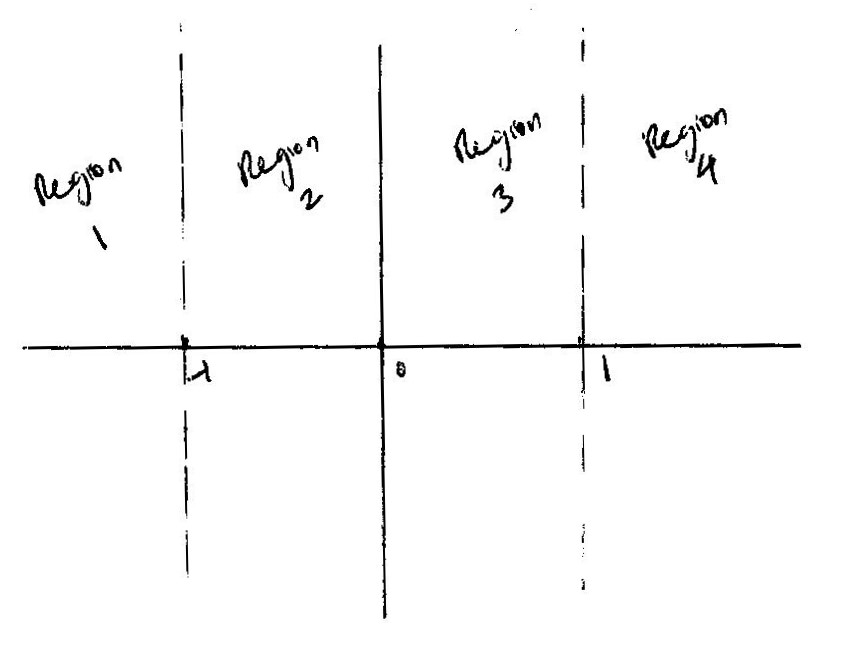
\includegraphics[scale = 0.75]{./_Figures/S07Q5c.jpg}
\end{center}
%
%
%
Thus characteristics don't cross before time $t = 1/a$ for characteristics that start in Regions 1, 2, and 4.
Consider two characteristics that start at $y_{1}$ and $y_{2}$ with $y_{1}, y_{2} \in (0, 1)$. We want to compute
when they crash. (In more ``traditional" notation for method of characteristics, $y_{1}$ is our $(x_{0})_{1}$ and $y_{2}$ is our $(x_{0})_{2}$.)
We want to solve for $t$ in
\begin{align*}
-\frac{2}{a}\ln(1 - at(1 - y_{1})) + y_{1} &= -\frac{2}{a}\ln(1 - at(1 - y_{2})) + y_{2}\\
\frac{2}{a}\ln\frac{1 - at(1 - y_{2})}{1 - at(1 - y_{1})} &= y_{2} - y_{1}\\
1 - at(1 - y_{2}) &= e^{\frac{a}{2}(y_{2} - y_{1})}(1 - at(1 - y_{1}))
\end{align*}
and hence the time when two characteristics that start at $y_{1}$ and $y_{2}$ with $y_{1}, y_{2} \in (0, 1)$ crash is
$$t = \frac{1 - e^{\frac{a}{2}(y_{2} - y_{1})}}{-ae^{\frac{a}{2}(y_{2} - y_{1})}(1 - y_{1}) + a(1 - y_{2})}.$$
Now let $y_{2} = 1/(na)$. Then
\begin{align*}
\lim_{y_{1} \rightarrow 1/(na)}&\frac{1 - e^{\frac{a}{2}(y_{2} - y_{1})}}{a(1 - y_{2}) - ae^{\frac{a}{2}(y_{2} - y_{1})}(1 - y_{1})} = \lim_{y_{1} \rightarrow 1/(na)}\frac{-e^{\frac{a}{2}(y_{2} - y_{1})}(-\frac{a}{2})}{-ae^{\frac{a}{2}(y_{2} - y_{1})}(-\frac{a}{2})(1 - y_{1}) - ae^{\frac{a}{2}(y_{2} - y_{1})}(-1)}\\
&= \lim_{y_{1} \rightarrow 1/(na)}\frac{a/2}{\frac{a^{2}}{2}(1 - \frac{1}{na}) + a} = \frac{a}{a^{2}(1 - \frac{1}{na}) + a} = \frac{1}{a + (1 - \frac{1}{n})} < \frac{1}{a}.
\end{align*}
Now choose $n$ sufficiently large such that $1/(na) < 1$.
Then the above argument shows that if we have a characteristic that starts at $1/(na)$ and another one that starts arbitrarily close,
then these two characteristics crash before time $1/a$. Therefore we cannot solve for $x = x(y, t)$
for all time in $[0, 1/a)$.
\begin{rem}
The technique of analyzing two arbitrarily close characteristics and computing when they crash is crucial to solving
Fall 2015, \#8. \hfill\qed
\end{rem}

\subsection*{Solution to Spring 2007, \#6}
We omit the solution to Problem $6(d)$.
\subsubsection*{Solution to $(a)$}
We have
$$-Cu + u^{3} - u^{2} + u''' = C_{1}.$$
Then
\begin{align*}
-Cu_{r} + u_{r}^{3} - u_{r}^{2} &= C_{1}\\
-Cu_{\ell} + u_{\ell}^{3} - u_{\ell}^{2} &= C_{1}.
\end{align*}
Thus
\begin{align*}
-Cu_{r} + Cu_{\ell} + u_{r}^{3} - u_{\ell}^{3} - u_{r}^{2} + u_{\ell}^{2} &= 0\\
-C(u_{r} - u_{\ell}) + (u_{r} - u_{\ell})(u_{r}^{2} + u_{r}u_{\ell} + u_{\ell}^{2}) - (u_{r} - u_{\ell})(u_{r} + u_{\ell}) &= 0.
\end{align*}
Since $u_{r} \neq u_{\ell}$,
$$-C + (u_{r}^{2} + u_{r}u_{\ell} + u_{\ell}^{2}) - (u_{r} + u_{\ell}) = 0$$
and hence
$$C = (u_{r}^{2} + u_{r}u_{\ell} + u_{\ell}^{2}) - (u_{r} + u_{\ell}).$$
\hfill\qed

\subsubsection*{Solution to $(b)$}
We have
$$C_{1} = -u_{r}(u_{r}^{2} + u_{r}u_{\ell} + u_{\ell}^{2}) + u_{r}(u_{r} + u_{\ell}) + u_{r}^{3} - u_{r}^{2}.$$
Note that this will also give a condition relating $u_{\ell}$ and $u_{r}$ since we can also use the equation relating
$u_{\ell}$ with $C_{1}$ in part $(a)$ to get a (slightly) different expression for $C_{1}$ and these two different expressions
of $C_{1}$ must be equal.
\hfill\qed

\subsubsection*{Solution to $(c)$}
The system can be written as $x' = y$, $y' = z$, $z' = C_{1} + Cx - x^{2} + x^{2}$. The equilibrium points occur
at $\{(a, 0, 0): a^{3} - a^{2} - Ca - C_{1} = 0\}$.
\hfill\qed

\subsection*{Solution to Spring 2007, \#7}
This problem is a good illustration of using integration by parts to obtain decay in integral expressions.
We will assume $\phi$ to be smooth (otherwise we cannot obtain such nice decay).

\subsubsection*{Solution to $(a)$}
We observe that
$$\frac{d}{dx}e^{ik\phi(x)} = e^{ik\phi(x)}ik\phi'(x)$$
and hence
\begin{align}\label{s077star}
\frac{1}{ik\phi'(x)}\frac{d}{dx}e^{ik\phi(x)} = e^{ik\phi(x)}.
\end{align}
Thus
\begin{align*}
\int_{\R}e^{ik\phi(x)}a(x)\, dx& = \int_{\R}\frac{1}{ik\phi'(x)}\frac{d}{dx}e^{ik\phi(x)}a(x)\, dx\\
& = \frac{1}{ik}\int_{\R}(\frac{d}{dx}e^{ik\phi(x)})\frac{a(x)}{\phi'(x)}\, dx = -\frac{1}{ik}\int_{\R}e^{ik\phi(x)}\frac{d}{dx}(\frac{a(x)}{\phi'(x)})\, dx.
\end{align*}
Since $\phi'(x)$ does not vanish for $|x| \leq R$, $(a(x)/\phi'(x))'$ is once again smooth and vanishes for $|x| > R$. Thus using \eqref{s077star} repeatedly
and following the same process as in the above centered equations yields that
$$\abb{\int_{\R}e^{ik\phi(x)}a(x)\, dx} \lsm_{N} k^{-N}.$$
(Recall here the notation ``$\lsm_{N}$" means ``$\leq C_{N}$" where $C_{N}$ is a constant only depending on $N$.)
\hfill\qed

\subsubsection*{Solution to $(b)$}
It suffices to prove that the derivative of $\phi(\alpha) := x\sin\alpha - y\cos\alpha - \alpha$ does not vanish for $|\alpha| \leq R$.
We have
$\phi'(\alpha) = x\cos\alpha + y\sin\alpha - 1$. For $x^{2} + y^{2} < 1$, we have
$$\abn{x \cos\alpha + y\sin\alpha} \leq \abn{(x, y) \cdot (\cos\alpha, \sin\alpha)} \leq (x^{2} + y^{2})^{1/2} < 1.$$
Thus $\phi'(\alpha)$ is never $0$ and hence $|u(x, y, k)| \lsm_{k} k^{-N}$ for all $N$ on $x^{2} + y^{2} < 1$.
\hfill\qed

\subsubsection*{Solution to $(c)$}
This problem is the method of stationary phase (see for example the book by Bender and Orszag).
We have
$$u(1, 0, k) = \int_{\R}e^{ik(\sin\alpha - \alpha)}a(\alpha)\, d\alpha = \int_{-\pi}^{\pi}e^{ik(\sin x - x)}a(x)\, dx.$$
We first have the following lemma which is similar in spirit to Part $(a)$
\begin{lemma}\label{s077lem1}
If $\psi' \neq 0$ on $[a, b]$ with $\vp, \psi$ smooth (and if one of $a, b$ is $\pm\infty$, $\vp/\psi'$ needs to have bounded derivative),
then
$$\int_{a}^{b}e^{ik\psi(t)}\vp(t)\, dt = O(\frac{1}{k}).$$
\end{lemma}
\begin{proof}
Note that $\frac{d}{dt}e^{ik\psi(t)} = ik\psi'(t)e^{ik\psi(t)}$. Then
\begin{align*}
\int_{a}^{b}e^{ik\psi(t)}\vp(t)\, dt = \int_{a}^{b}\frac{1}{ik\psi'(t)}\vp(t)\frac{d}{dt}e^{ik\psi(t)}\, dt = \frac{\vp(t)e^{ik\psi(t)}}{ik\psi'(t)}\bigg]_{t = a}^{b} - \int_{a}^{b}\frac{1}{ik}\frac{d}{dt}(\frac{\vp(t)}{\psi'(t)})e^{ik\psi(t)}\, dt.
\end{align*}
Therefore
$$\abb{\int_{a}^{b}e^{ik\psi(t)}\vp(t)\, dt} = O(\frac{1}{k}).$$
This completes the proof the lemma.
\end{proof}

Let $\delta < 0.01$ to be chosen later. We have
$$\int_{\R}e^{ik(\sin x - x)}a(x)\, dx = \int_{-\pi}^{\pi}e^{ik(\sin x - x)}a(x)\, dx.$$
Close to $0$,
\begin{align*}
e^{ik(\sin x - x)}a(x) &= e^{ik(-\frac{x^{3}}{3!} + O(x^{5}))}(a(0) + a'(0)x + O(x^{2}))\\
& = e^{-ikx^{3}/3!}(a(0)(1 + ikO(x^{5})) + O(x)) = a(0)e^{-ikx^{3}/3!} + e^{-ikx^{3}/3!}O(x)
\end{align*}
where the last equality is because $|x|^{5} \ll |x|$ for $x$ close to $0$.
Then with $\delta$ smaller than the radius of convergence for the power series expansion of $e^{ik(\sin x - x)}a(x)$ about $x = 0$,
\begin{align*}
\int_{-\pi}^{\pi}&e^{ik(\sin x - x)}a(x)\, dx\\
& = (\int_{-\pi}^{-\delta} + \int_{\delta}^{\pi})e^{ik(\sin x - x)}a(x)\, dx + \int_{-\delta}^{\delta}e^{ik(\sin x - x)}a(x)\, dx\\
&=\int_{-\delta}^{\delta}e^{ik(\sin x - x)}a(x)\, dx + O(1/k)\\
&= \int_{-\delta}^{\delta}a(0)e^{-ikx^{3}/3!}\, dx + O(\int_{-\delta}^{\delta}xe^{-ikx^{3}/3!}\, dx) + O(1/k)\\
&= \int_{\R}a(0)e^{-ikx^{3}/3!}\, dx - (\int_{-\infty}^{-\delta} + \int_{\delta}^{\infty})a(0)e^{-ikx^{3}/3!}\, dx + O(\int_{-\delta}^{\delta}xe^{-ikx^{3}/3!}\, dx) + O(1/k).
\end{align*}
By the lemma,
$$(\int_{-\infty}^{\delta} + \int_{\delta}^{\infty})a(0)e^{-ikx^{3}/3!}\, dx = O(1/k).$$
We also have
$$\int_{-\delta}^{\delta}xe^{-ikx^{3}/3!}\, dx = \int_{\R}xe^{-ikx^{3}/3!}\, dx - \int_{-\infty}^{-\delta}xe^{-ikx^{3}/3!}\, dx - \int_{\delta}^{\infty}xe^{-ikx^{3}/3!}\, dx$$
and
\begin{align*}
\int_{\delta}^{\infty}xe^{-ikx^{3}/3!}\, dx &= \int_{\delta}^{\infty}x\frac{1}{ik(-\frac{x^{2}}{2})}\frac{d}{dx}e^{-ikx^{3}/3!}\, dx= \int_{\delta}^{\infty}-\frac{2}{ikx}\frac{d}{dx}e^{-ikx^{3}/3!}\, dx\\
& = -\frac{2}{ikx}e^{-ikx^{3}/3!}\bigg]_{x = \delta}^{\infty} - \frac{2}{ik}\int_{\delta}^{\infty}\frac{1}{x^{2}}e^{-ikx^{3}/3!}\, dx = O(1/k).
\end{align*}
Similarly, $$\int_{-\infty}^{-\delta}xe^{-ikx^{3}/3!}\, dx = O(1/k).$$
Finally,
$$\int_{\R}xe^{-ikx^{3}/3!}\, dx = \frac{1}{k^{2/3}}\int_{\R}e^{-iu^{3}/3!}\, du = O(1/k^{2/3}).$$
Putting all the above computations together yields
\begin{align*}
\int_{\R}e^{ik(\sin x - x)}\, dx = a(0)\int_{\R}e^{-ikx^{3}/3!}\, dx + O(1/k^{2/3}) = \frac{a(0)}{k^{1/3}}\int_{\R}e^{-iu^{3}/3!}\, du + O(1/k^{2/3}).
\end{align*}
\hfill\qed

\subsection*{Solution to Spring 2007, \#8}
\subsubsection*{Solution to $(a)$}
Since $\int_{\R^n}u(x, t)\, dx$ is conserved, $\frac{d}{dt}\int_{\R^{n}}u(x, t)\, dx = 0$. Since $u(x, t) = t^{-\alpha}U(x/t^{\beta})$,
\begin{align*}
0 = \frac{d}{dt}\int_{\R^{n}}t^{-\alpha}U(x/t^{\beta})\, dx = \frac{d}{dt}\int_{\R^{n}}t^{-\alpha + \beta n}U(x)\, dx = \bigg(\int_{\R^{n}}U(x)\, dx\bigg)\frac{d}{dt}t^{-\alpha + \beta n}
\end{align*}
which implies that
\begin{align}\label{s078cond1}
\alpha = \beta n.
\end{align}
\hfill\qed

\subsubsection*{Solution to $(b)$}
We have $u(\mb{x}, t) = t^{-\alpha}U(\mb{x}/t^{\beta})$. Then
\begin{align*}
u_{t} &= -\alpha t^{-\alpha - 1}U(\eta) + t^{-\alpha}\del_{\eta}U \cdot \eta_{t}\\
& = -\alpha t^{-\alpha - 1}U(\eta) + t^{-\alpha}\nabla U \cdot \mb{x}(-\beta t^{-\beta - 1})\\
& = -\alpha t^{-\alpha - 1}U(\eta) - t^{-\alpha - 1}\beta \del U \cdot \eta.
\end{align*}
We also have
\begin{align*}
\Delta(u^{m}) &= \sum_{i}\pr_{x_{i}x_{i}}(u^{m}) = \sum_{i}\pr_{x_{i}}(mu^{m - 1}u_{x_{i}})\\
& = m\sum_{i}(m - 1)u^{m - 2}u_{x_{i}}^{2} + u^{m - 1}u_{x_{i}x_{i}} = m(m - 1)u^{m - 2}\abn{\del_{x}u}^{2} + mu^{m - 1}\Delta_{x}u.
\end{align*}
With $u(\mb{x}, t) = t^{-\alpha}U(\mb{x}/t^{\beta})$, then
$\del_{x}u = t^{-\alpha - \beta}\del_{\eta}U$ and $\lap_{x}u = t^{-\alpha - 2\beta}\lap_{\eta}U.$
Thus
\begin{align*}
\Delta(u^{m}) &= m(m - 1)t^{-\alpha(m - 2)}U(\eta)^{m - 2}t^{-2\alpha - 2\beta}\abn{\del U}^{2} + mt^{-\alpha(m - 1)}U(\eta)^{m - 1}t^{-\alpha- 2\beta}\lap U\\
&= m(m - 1)U(\eta)^{m - 2}\abn{\del U}^{2}t^{-\alpha m - 2\beta} + mU(\eta)^{m - 1}\Delta U t^{-\alpha m - 2\beta}.
\end{align*}
Since $u_{t} = \Delta(u^{m})$, we need
\begin{align}\label{s078cond2}
-\alpha - 1 = -\alpha m - 2\beta
\end{align}
Then
\begin{align*}
-\alpha U(\eta) - \beta \del U \cdot \eta = m(m - 1)U(\eta)^{m - 2}\abn{\del U}^{2} + mU(\eta)^{m - 1}\lap U = \lap_{\eta}U.
\end{align*}
Therefore \eqref{s078cond1} and \eqref{s078cond2} imply $$\alpha = \frac{n}{(m - 1)n + 2}\quad\quad \text{ and } \quad\quad \beta = \frac{1}{(m - 1)n + 2}$$
and $U(\eta)$ satisfies
$$\alpha U(\eta) + \beta\nabla U \cdot \eta + \Delta_{\eta}U = 0.$$
Thus $C_{1} = \alpha$ and $C_{2} = \beta$.
\hfill\qed

\subsubsection*{Solution to $(c)$}
If we look for a radial solution $U(\eta) = f(|\eta|) = f(r)$, then we will solve
\begin{align*}
\alpha f + \beta rf' + (f^{m})'' + \frac{n - 1}{r}(f^{m})' &= 0\\
\beta nf + \beta rf' + (f^m)'' + \frac{n - 1}{r}(f^m)' &= 0\\
\beta nr^{n - 1}f + \beta r^{n}f' + r^{n - 1}(f^{m})'' + (n - 1)r^{n - 2}(f^{m})' &= 0\\
(\beta r^{n}f)' + (r^{n - 1}(f^{m})')' &= 0.
\end{align*}
Since we are just finding a family of solutions, let $f$ such that
\begin{align*}
\beta r^{n}f + (r^{n - 1}(f^{m})')' &= 0\\
\beta r^{n}f + r^{n - 1}mf^{m - 1}f' &= 0\\
\beta r + mf^{m - 2}f' &= 0\\
\int mf^{m - 2}\, df &= \int -\beta r\, dr
\end{align*}
which implies that
$$\frac{m}{m - 1}f^{m - 1} = -\frac{1}{2}\beta r^{2} + C$$
which upon rearranging yields
$$f = ([C - \frac{1}{2}\beta r^{2}]\frac{m - 1}{m})_{+}^{1/(m - 1)}$$
where given a function $F$, $F_{+} := \max(F, 0)$ (we take the positive part since we want $U$ to be nonnegative).
Therefore
\begin{align}\label{s078sol}
u(x, t) = \frac{1}{t^{\alpha}}(\frac{m - 1}{m}[C - \frac{1}{2}\beta\frac{|x|^{2}}{t^{2\beta}}])_{+}^{1/(m - 1)}.
\end{align}
\hfill\qed

\subsubsection*{Solution to $(d)$}
We now need to find $C$ such that $u(x, t)$ given by \eqref{s078sol} is such that $\int u(x, t)\, dx = 1$.
Let $$L = L(t) = \sqrt{\frac{2Ct^{2\beta}}{\beta}}.$$
We have
$$1 = \int_{|x| \leq L(t)}\frac{1}{t^{\alpha}}(\frac{m - 1}{m}[C - \frac{1}{2}\beta\frac{|x|^{2}}{t^{2\beta}}])^{1/(m - 1)}\, dx.$$
Then
\begin{align*}
t^{\alpha}(\frac{m}{m - 1})^{1/(m - 1)} &= \int_{|x| \leq L(t)}(C - \frac{\beta}{2t^{2\beta}}|x|^{2})^{1/(m - 1)}\, dx\\
&= \int_{S^{n - 1}}\, d\sigma\int_{0}^{L(t)}(C - \frac{\beta}{2t^{2\beta}}r^{2})^{1/(m - 1)}r^{n - 1}\, dr\\
&= \int_{S^{n - 1}}\, d\sigma\int_{0}^{L(t)}(\frac{C\cdot 2t^{2\beta}}{\beta} - r^{2})^{1/(m -1)}(\frac{\beta}{2t^{2\beta}})^{1/(m - 1)}r^{n- 1}\, dr
\end{align*}
and hence
\begin{align*}
\frac{(\frac{2t^{2\beta}}{\beta})^{1/(m - 1)}t^{\alpha}(\frac{m}{m - 1})^{1/(m - 1)}}{\int_{S^{n - 1}}\, d\sigma} = \int_{0}^{L(t)}(L(t)^{2} - r^{2})^{1/(m - 1)}r^{n - 1}\, dr.
\end{align*}
Let $r = L\sin\ta$, then $dr = L\cos\ta\, d\ta$ and
\begin{align*}
\int_{0}^{L}(L^{2} - r^{2})^{1/(m - 1)}r^{n - 1}\, dr &= \int_{0}^{\pi/2}(\cos\ta)^{2/(m - 1)}L^{n - 1}(\sin \ta)^{n - 1}L\cos\ta\, d\ta\\
& = L^{n}\int_{0}^{\pi/2}(\cos\ta)^{(m + 1)/(m - 1)}(\sin\ta)^{n - 1}\, d\ta.
\end{align*}
Thus
\begin{align*}
\displaystyle C = \bigg[\frac{(\frac{2t^{2\beta}}{\beta})^{1/(m - 1)}t^{\alpha}(\frac{m}{m - 1})^{1/(m - 1)}}{\int_{S^{n - 1}}\, d\sigma\int_{0}^{\pi/2}(\cos\ta)^{(m + 1)/(m - 1)}(\sin\ta)^{n - 1}\, d\ta}\bigg]^{2/n}\frac{\beta}{2t^{2\beta}}
\end{align*}
and with this $C$,
$$u(x, t) = t^{-\alpha}(\frac{m - 1}{m}[C - \frac{1}{2}\beta\frac{|x|^{2}}{t^{2\beta}}])_{+}^{1/(m - 1)}$$
is such that $\int u(x, t)\, dx = 1$.
\hfill\qed


\newpage

\section{Appendices}

\subsection*{Sturm-Liouville Theory \small{(a brief review)}}
\label{SturmLiouville}

The \emph{regular} Sturm-Liouville problem is given by
\[
\left\{
\begin{array}{l}
(p(x)u')' + q(x)u = -\lambda r(x) u,  \quad a < x < b \\
B_a[u] := \alpha u(a) + \beta u'(a) = 0 \\
B_b[u] := \gamma u(b) + \delta u'(b) = 0
\end{array}
\right.
\]
where $p,p',q,r \in C[a,b]$, $p,r > 0$, $\alpha, \beta, \gamma, \delta \in \R$, $|\alpha|+|\beta| > 0$, $|\gamma| + |\delta| > 0$.

If we define $Lu := (p(x)u')' + q(x) u$ as an operator on the space $V = \{ u \in C^2([a,b]) \, | \, B_a[u] = B_b[u] = 0 \}$, we can show $L$ is self-adjoint with respect to the standard inner product $\langle f,g \rangle = \int_a^b f(x)\overline{g(x)} \, dx$. Thus, the Sturm-Liouville problem would be the weighted eigenvalue problem $Lu = \lambda r(x) u$.

However, if we rewrite the ODE of the Sturm-Liouville problem as
\[
\frac{1}{r(x)}\left[ (p(x)u')' + q(x)u \right]= -\lambda u
\]
and define $\tilde{L}u := \frac{1}{r(x)}\left[ (p(x)u')' + q(x)u \right]$ as an operator on $V$, we can show that $\tilde{L}$ is self-adjoint with respect to the weighted inner product $\langle f,g \rangle_{r(x)} = \int_a^b f(x) \overline{g(x)} r(x) \, dx$. In this case, the Sturm-Liouville problem would be a regular eigenvalue problem on a weighted inner product.

Either way, we get that our Sturm-Liouville operator is self-adjoint, which means we have some very nice properties:
\begin{enumerate}
\renewcommand{\labelenumi}{(\alph{enumi})}
\item $L$ is self-adjoint with respect to the standard inner product ($\tilde{L}$ is self-adjoint with respect to the inner product weighted with $r(x)$)

\item The eigenvalues of $L$ and $\tilde{L}$ are real and simple.

\item Eigenfunctions corresponding to distinct eigenvalues are orthogonal.

\item The set of eigenvalues form a sequence $\lambda_0 < \lambda_1 < \cdots < \lambda_n < \cdots$ with $\lambda_n \to \infty$.

\item Let $v_n$ denote the $n$th eigenfunction corresponding to $\lambda_n$. The Rayleigh quotient allows us to find the eigenvalues:
$$ \lambda_0 = \min_{u \in V} -\dfrac{\langle u, Lu \rangle}{\langle u, u \rangle_{r(x)}}, \quad \quad \lambda_{N+1} = \min_{u \in W_N^{\perp}}   -\dfrac{\langle u, Lu \rangle}{\langle u, u \rangle_{r(x)}} $$
or
$$ \lambda_0 = \min_{u \in V} -\dfrac{\langle u, \tilde{L}u \rangle_{r(x)}}{\langle u, u \rangle_{r(x)}}, \quad \quad \lambda_{N+1} = \min_{u \in W_N^{\perp}}   -\dfrac{\langle u, \tilde{L}u \rangle_{r(x)}}{\langle u, u \rangle_{r(x)}} $$
where $W_N^{\perp} = \{ u \, | \, \langle u, v_n \rangle = 0 \,\, \text{for} \,\, n = 0, 1, \dots, N \}$. It is important to note that the inner product in the denominator of the Rayleigh quotient here is always weighted with $r(x)$ --- this is NOT a typo!

\item The set of eigenfunctions $\{v_n\}$ corresponding to the eigenvalues $\lambda_n$ form a complete orthogonal basis of $V$.
\end{enumerate}

I don't have a reference for (d), but assuming that result stated in (d) is true, (e) is not too difficult to prove (requires some calculus of variations and integration by parts). Then, the result of (f) follows from both (d) and (e). If you're interested, here's a proof for (f): \url{https://people.math.osu.edu/gerlach.1/math/BVtypset/node76.html}.


One final important fact to know --- under some mild conditions, we may write any second-order ODE into Sturm-Liouville form. Consider the following second-order ODE
$$a(x) y'' + b(x) y' + c(x) y = -\lambda w(x) y, \quad \quad a < x < b $$
where $a(x) > 0$ on $(a,b)$. Furthermore, suppose we have boundary conditions at $x=a$ and $x=b$. Then,
$$a(x) y'' + b(x) y' + c(x) y = -\lambda w(x) y  \quad \implies \quad y'' + \frac{b(x)}{a(x)} y' + \frac{c(x)}{a(x)}y = -\lambda \frac{w(x)}{a(x)} y $$
For ease of notation, define $\tilde{b}(x) := \frac{b(x)}{a(x)}$, $\tilde{c}(x) := \frac{c(x)}{a(x)}$, $r(x) := \frac{w(x)}{a(x)}$. Then, multiplying both sides of the ODE by the integrating factor $k(x) = e^{\int \tilde{b}(x) dx}$ yields
\begin{align*}
	 y'' +\tilde{b}(x) y' + \tilde{c}(x) y = -\lambda r(x) y \quad &\implies \quad \left( k(x) y' \right)' + k(x) \tilde{c}(x) y = -\lambda k(x) r(x) y \\
	 &\implies \quad \frac{1}{k(x)r(x)} \left[ \left( k(x) y' \right)' + k(x) \tilde{c}(x) y \right] = -\lambda y
\end{align*}
which is now Sturm-Liouville problem. Remember, depending on what form of the operator we use, we need to weight the inner product correctly.

\sub{Analysis ``tricks" for nonlinear equations}
\noindent Here we record two ideas that Peter and I found useful while proving results about PDEs (especially nonlinear ones).
\begin{enumerate}[$(1)$]
\item \emph{In bounded domains, use the $L^{p}$ norm to control the $L^{\infty}$ norm.}

Often in problems (such as Spring 2008, \#7; Spring 2010, \#2, or Spring 2014, \#2), one needs to control data about $\sup_{x \in \Om}\abn{u(x, t)}$.
That is if $u$ is a smooth solution, we want to control the $L_{x}^{\infty}$ norm of $u(x, t)$ (in other words, the $L^{\infty}$ norm in the $x$
variable, thus our bounds will depend on $t$).
A typical way of handling this is to prove a maximum principle or Hopf's lemma for the problem. But sometimes it is not clear on how to
prove such a lemma especially if the problem is a nonlinear PDE (in which case a first time argument might help).
If $\Om$ is bounded, then we can use the following fact about $L^{p}$ norms:
\begin{lemma}
If $f(x)$ is a smooth function and $\Om \subset \R^{d}$ is bounded, then
$\lim_{p \rightarrow \infty}\nms{f}_{L^{p}(\Om)} = \nms{f}_{L^{\infty}(\Om)}.$
\end{lemma}
\begin{proof}
Since $f$ is smooth and $\Om$ is bounded, $\nms{f}_{L^{1}} < \infty$.
By how the $L^{\infty}$ norm is defined, $\abs{f(x)} \leq \nm{f}_{L^{\infty}}$ for almost every $x \in \Om$. Observe that for $p > 1$,
\begin{align*}
\nm{f}_{L^{p}} = \left(\int_{\Om}\abs{f}^{p}\, d\mu\right)^{1/p} &= \left(\int_{\Om}\abs{f}^{p - 1}\abs{f}\, d\mu\right)^{1/p}\\
& \leq \nm{f}_{L^{\infty}}^{1 - \frac{1}{p}}\left(\int_{\Om}\abs{f}\, d\mu\right)^{1/p} = \nm{f}_{L^{\infty}}^{1 - \frac{1}{p}}\nm{f}_{L^{1}}^{1/p}.
\end{align*}
Therefore $$\limsup_{p \rightarrow \infty}\nm{f}_{L^{p}} \leq \limsup_{p \rightarrow \infty}\nm{f}_{L^{\infty}}^{1 - \frac{1}{p}}\nm{f}_{L^{1}}^{1/p} = \nm{f}_{L^{\infty}}.$$
By how the $L^{\infty}$ is defined, for every $\vep > 0$, there exists a $\delta > 0$ such that
$\mu(\{x \in \Om: \abs{f(x)} \geq \nm{f}_{L^{\infty}} - \vep\}) \geq \delta$. Then
$$\nm{f}_{L^{p}} = \left(\int_{\Om}\abs{f}^{p}\, d\mu\right)^{1/p} \geq \delta^{1/p}(\nm{f}_{L^{\infty}} - \vep).$$
Therefore $$\liminf_{p \rightarrow \infty}\nm{f}_{L^{p}} \geq \nm{f}_{L^{\infty}} - \vep$$ and letting $\vep \rightarrow 0$
yields that $\liminf_{p \rightarrow \infty}\nm{f}_{L^{p}} \geq \nm{f}_{L^{\infty}}$. Thus we have $\lim_{p \rightarrow \infty}\nm{f}_{L^{p}} = \nm{f}_{L^{\infty}}$.
\end{proof}
Thus if we know smoothing about $\nms{u}_{L^{p}_{x}(\Om)} \leq M$ for some $M$ (where $M$ can depend on $p$ and $t$), then
by the above lemma,
\ba
\sup_{x \in \Om}\abn{u(x, t)} = \nms{u}_{L^{\infty}_{x}(\Om)} = \lim_{p\rightarrow \infty}\nms{u}_{L^{p}_{x}(\Om)} \leq M.
\ea
This approach can look slightly more complicated (for example, usually one works with $E(t) := \int_{\Om}|u|^{p}\, dx$ which is $\nms{u}_{L^{p}_{x}(\Om)}^{p}$
and then take the time derivative), but it reduces the problem to just straightforward computation and does not require any clever observations or substitutions
to find a maximum principle for the problem.

\item \emph{When proving a strict inequality about the behavior of a (smooth) solution, consider the first time when the inequality fails.}

This is what Peter and I called the ``first time argument" in our solutions. Often one wants to show a strict inequality regarding the solution (for example,
our solution $u > 0$ for all space and time)\footnote{If ones wants to show that $u \geq 0$, then one way to turn this into a strict inequality is by showing for every $\vep > 0$,
$u > -\vep$.} The first time argument is crucial in Spring 2008, \#7; Fall 2011, \#2 and \#4; Fall 2014, \#7. Combining this with a perturbation
allows one to prove maximum principle type results for nonlinear PDEs.

The idea of the first time argument is as follows. Let $u$ be a smooth solution to a given PDE. Suppose we know at time $t = 0$, $u(x, t) > 0$ for all $x$ in our domain.
We want to prove that $u > 0$ always. Suppose this was not true. Since $u$ is a smooth solution, there exists a first time $t_{0}$ and a minimal $x_{0}$ (the minimality of $x_{0}$
is not so crucial) such that $u(x_{0}, t_{0}) = 0$. Since $u$ was initially positive and $t = t_{0}$ was the \emph{first} time my solution hits 0,
then $u(x, t') > 0$ for all $t' < t_{0}$ and $u(x, t_{0}) \geq 0$ for all $x$. Then $u_{t}(x_{0}, t_{0}) \leq 0$ and since $x = x_{0}$ is local minimum of $u(\cdot, t_{0})$,
$\Delta_{x}u(x_{0}, t_{0}) \geq 0$. Now analyzing the PDE at the point $(x_{0}, t_{0})$ should give a contradiction (if not, perhaps apply a perturbation such as $\pm \vep t$ or $\pm \vep e^{\pm \ld x}$).
\end{enumerate}
\end{document}


\end{document}
